% to create the package use the following commands
% pdflatex GBTog ; makeglos.pl GBTog; makeindex GBTog.idx; pdflatex GBTog;  pdflatex GBTog
% rm -fr GBTog/*
% latex2html -no_math -html_version 4.0,math,frame -local_icons -white -show_section_numbers -split 5 GBTog
% put documents in /home/www.gb.nrao.edu/content/gbtprops/obsman/

\documentclass{book}

% The next two packages are needed when compiling from GB linux systems
%\usepackage{graphicx} %incompatible driver with pdflatex compiler on sharelatex
%\usepackage{html}

% packages that will be needed
\usepackage[dvips]{color}
\usepackage{lscape}
\usepackage{ifthen}
\usepackage{listings}
\usepackage{makeidx}
\usepackage{glossaries}
\usepackage{robustindex}
\usepackage{rotating}
\usepackage{SIunits}
\usepackage{enumitem}
\usepackage{subfig}
\usepackage{wrapfig}
\usepackage{textcomp}
\usepackage{setspace}
\usepackage{courier}
\usepackage{chngcntr}
\usepackage{booktabs}
\usepackage{multirow}
\usepackage{hhline}
\usepackage{dcolumn}
\usepackage{caption}
\usepackage{amsmath}
\usepackage{color}
\usepackage{hyperref}
\usepackage{sectsty}
\usepackage{tikz}
\usepackage{calc}
\usepackage{floatrow}
\usepackage{float}

\floatstyle{plaintop}
\restylefloat{table}
\captionsetup[table]{aboveskip=0pt,belowskip=0pt,skip=0pt} 

\graphicspath{ {images/} }  %path for images
\lstset{inputpath=code/} %path for code

\pagecolor{white}

% Basic page layout (see LaTeX book page 163):
%
%               size 8.5 x 11 inch pages
%    odd side margin 1.25 inches
%   even side margin 1.25 inches
%         top margin 1.25 inch
%        text height 9 inches
%          tex width 6.25 inches
%
%
% assumed to be set up for single-sided printing, so that the \markright
% command (i.e. right-hand page) is used. Left hand side of page contains
% contents of \mydocmarkright, right hand side, page number.


\setlength {\textwidth}      {6.25in}
\setlength {\textheight}     {9in}
\setlength {\topmargin}      {-0.55in}
\setlength {\oddsidemargin}  {0.25in}
\setlength {\evensidemargin} {0.25in}
% 
\pagestyle{myheadings}
%
\setlength {\parindent}      {0.25in}
\setlength {\parskip}        {\medskipamount}
\setlength {\unitlength}     {1in}

%column type for tables that aligns by decimal point
\newcolumntype{d}{D{.}{.}{-1}}

% define colors
\definecolor{coverpages}{rgb}{0.5625,0.8125,1.0} %nraoblue atm.
\definecolor{seccolor}{rgb}{0.0000,0.1992,0.3984}
\definecolor{subcolor}{rgb}{0.1953,0.1953,0.8045}
\definecolor{subsubcolor}{rgb}{0.0000,0.4961,1.0}
\definecolor{nraoblue}{rgb}{0.5625,0.8125,1.0}
\definecolor{configBackground}{rgb}{0.97,0.97,1.0}
\definecolor{catalogBackground}{rgb}{1.0,1.0,0.95}
\definecolor{sbBackground}{rgb}{0.98,1.0,0.98}
\definecolor{pythonCode}{rgb}{0,0,0}
\definecolor{pythonDecorators}{rgb}{0.5,0.5,0.5}
\definecolor{pythonNumbers}{rgb}{0.5,0,0}
\definecolor{pythonArray}{rgb}{0,0.3,0.8}
\definecolor{pythonKeywords}{rgb}{0.1,0,0.5}
\definecolor{pythonSelf}{rgb}{0,0,0}
\definecolor{pythonStrings}{rgb}{0.7,0.0,0.6}
\definecolor{pythonTripleStrings}{rgb}{0.4,0.1,0.1}
\definecolor{pythonComments}{rgb}{0,0.35,0.1}
\definecolor{pythonBackquotes}{rgb}{0,0,0}
\definecolor{pythonClassname}{rgb}{0,0,0}
\definecolor{pythonFunctionName}{rgb}{0,0,0}
\definecolor{pythonOperators}{rgb}{0,0,0}

% checkmark
\def\checkmark{\tikz\fill[scale=0.4](0,.35)--(.25,0)--(1,.7)--(.25,.15)--cycle;} 

% Cool Buttons
\usetikzlibrary{shapes.geometric,shapes.symbols,shadows,calc}

\tikzstyle{astridbuttonstyle} = [ fill = black!30, draw = black!50,
                                  font={\sffamily}, text=black,
                                  top color=black!2, bottom color=black!10,
                                  rounded corners=0.75pt,
                                  inner ysep=2pt, inner xsep=2pt,
                                  baseline=(tempname.base)]

\tikzstyle{astridfixedbuttonstyle} = [ fill = black!30, draw = black!50,
                                       font={\sffamily}, text=black,
                                       top color=black!1, bottom color=black!20,
                                       rounded corners=0.75pt,
                                       baseline=(tempname.base),
                                       minimum height = 3ex, text height = 1.5ex,
                                       text depth = 0.25ex, text centered]

\tikzstyle{astridyellowbuttonstyle} = [ fill = yellow!30, draw = black!50,
                                        font={\sffamily}, text=black,
                                        top color=yellow!5, bottom color=yellow!45,
                                        rounded corners=0.75pt,
                                        inner ysep=2pt, inner xsep=2pt,
                                        baseline=(tempname.base)]

\tikzstyle{cleobuttonstyle} = [ fill = black!15, draw = black!15,
                                       font={\ttfamily\small}, text=black,
                                       inner ysep=2pt, inner xsep=2pt,
                                       baseline=(tempname.base)]

\newcommand*{\astridfixedbutton}[2]{
\begin{tikzpicture}[baseline=(tempname.base)]
\node[astridfixedbuttonstyle, text width={#2}] (tempname) {#1};
\end{tikzpicture}
}
\newcommand*{\astridbutton}[1]{
\begin{tikzpicture}[baseline=(tempname.base)]
\node[astridbuttonstyle] (tempname) {#1};
\end{tikzpicture}
}
\newcommand*{\astridyellowbutton}[1]{
\begin{tikzpicture}[baseline=(tempname.base)]
\node[astridyellowbuttonstyle] (tempname) {#1};
\end{tikzpicture}
}
\newcommand*{\cleobutton}[1]{
\begin{tikzpicture}[baseline=(tempname.base)]
\node[cleobuttonstyle] (tempname) {#1};
  \draw[black!5, fill=black!5, line width=0pt] ($ (tempname.north west) + (-0.75pt,0.75pt) $) rectangle
                               ($ (tempname.north east) + (0pt,0pt) $);
  \draw[black!5, fill=black!5, line width=0pt] ($ (tempname.north west) + (-0.75pt,0pt) $) rectangle
                               ($ (tempname.south west) + (0pt,-0.75pt) $);
  \draw[black!30, fill=black!30, line width=0pt] ($ (tempname.south west) + (0pt,0pt) $) rectangle
                                 ($ (tempname.south east) + (0.75pt,-0.75pt) $);
  \draw[black!30, fill=black!30, line width=0pt] ($ (tempname.south east) + (0.75pt,0pt) $) rectangle
                                 ($ (tempname.north east) + (0pt,0.75pt) $);
  \draw[black!5, fill=black!5, line width=0pt] ($ (tempname.north east) $) --
                 ($ (tempname.north east) + (0pt,0.75pt)$) --
                 ($ (tempname.north east) + (0.75pt,0.75pt)$) -- cycle;
  \draw[black!30, fill=black!30, line width=0pt] ($ (tempname.south west) $) --
                 ($ (tempname.south west) + (0pt,-0.75pt)$) --
                 ($ (tempname.south west) + (-0.75pt,-0.75pt)$) -- cycle;
\end{tikzpicture}
} %all that!....


% command for correct double quotes in pdf and in html versions
\newcommand{\dq}[1]{``#1''}
\newcommand{\sq}[1]{\lq{#1}\rq}
% straight quotation marks
\newcommand{\ssq}[1]{\textquotesingle{#1}\textquotesingle}
\newcommand{\sdq}[1]{\textquotesingle\textquotesingle{#1}\textquotesingle\textquotesingle}
% for tables
\newcommand{\myalign}[2]{\multicolumn{1}{#1}{#2}}


\font\btt=rm-lmtk10

%Headings
\chapterfont{\color{black}}
\sectionfont{\color{seccolor}\huge}
\subsectionfont{\color{subcolor}\Large}
\subsubsectionfont{\color{subsubcolor}\large}
% definition for subsubsubsection = topic
\newcommand{\txtblue}[1]{\textcolor{blue}{#1}}
\newcommand{\topic}[1]{\noindent{\txtblue{\textbf{
  \smallskip\center\Large #1}}}\addcontentsline{toc}{paragraph}{#1}}


% here's the stuff to get Astrid code looking kind of okay
\renewcommand{\lstlistingname}{Script}
\renewcommand{\lstlistlistingname}{List of \lstlistingname s}
\lstdefinelanguage{PythonAstrid}{
columns=fullflexible,
showspaces=false,
showtabs=false,
showstringspaces=false,
keepspaces=true,
captionpos=b,
frame=single,
framerule=1pt,
tabsize=4,
upquote=true,
% Basic
basicstyle=\ttfamily,
backgroundcolor=\color{configBackground},
% Comments
commentstyle=\color{pythonComments}\slshape,
% Strings
stringstyle=\color{pythonStrings},
identifierstyle=\color{pythonCode},
morecomment=[s][\color{pythonStrings}]{'}{'},
morecomment=[s][\color{pythonStrings}]{"}{"},
morecomment=[s][\color{pythonTripleStrings}]{"""}{"""},
morecomment=[s][\color{pythonTripleStrings}]{'''}{'''},
morecomment=[l][\color{pythonComments}]{\#},
% keywords
morekeywords={import,from,class,def,for,while,if,is,in,elif,else,
not,and,or,print,break,continue,return,access,as,del,
except,exec,finally,global,import,lambda,pass,print,raise,try,
assert,execfile,Track,OnOff,OffOn,AutoPeak,AutoPeakFocus,AutoOOF,
Balance,Slew,Catalog,Configure,Nod,Break,Location,Focus,Peak,
Slew,Tip,BalanceOnOff,Offset,OnOffSameHA,RALongMapWithReference,
RALongMap,DecLatMapWithReference,DecLatMap,PointMapWithReference,
PointMap,Daisy,Annotation,Break,Comment,GetUTC,GetLST,Now,WaitFor,
ChangeAttenuation,GetValue,SetValues,DefineScan,GetCurrentLocation,
SetSourceVelocity,Spider,Z17,CircleTrack,SubBeamNod},
keywordstyle={\color{pythonKeywords}\bfseries},
% additional keywords
morekeywords={[2]@invariant,pylab,numpy,np,scipy},
keywordstyle={[2]\color{pythonDecorators}\slshape},
emph={self},
emphstyle={\color{pythonSelf}\slshape},
%
}

%the glossary
\loadglsentries{GBTog_glossary}
\makenoidxglossaries


% start the document now
\begin{document}
\frontmatter
\setcounter{page}{0}

%
% the pdf book cover/title page
%

% set title information
\title{\txtseccolor{\Huge Observing With The Green Bank Telescope}}
\author{\txtseccolor{\Large GBT Scientific Staff}}
\date{\Large \txtseccolor{\today}}

%Define Frame for cover page
\newsavebox{\FrameCoverPage}
\newenvironment{FrameCover}[4]%
{\begin{lrbox}{\FrameCoverPage}\begin{minipage}[#1][#2][#3]{#4}}%
{\end{minipage}\end{lrbox}\fbox{\usebox{\FrameCoverPage}}}
\newcommand{\FramePix}[3][t]{\fbox{\begin{minipage}[#1]{#2} #3\end{minipage}}}

\colorbox{coverpages}{
\begin{FrameCover}{c}{8.5in}{t}{5.5in}
\vspace*{\stretch{1}}
\begin{center}
\textcolor{green}{\rule{\linewidth}{3.2mm}}
\textit{\Huge \bf Observing With The\\[5mm]
\Huge \bf Green Bank Telescope}
\textcolor{green}{\rule{\linewidth}{3.2mm}}
\end{center}

\vspace*{\stretch{1}}
\begin{center}
\FramePix[c]{4.5in}
{\bfseries 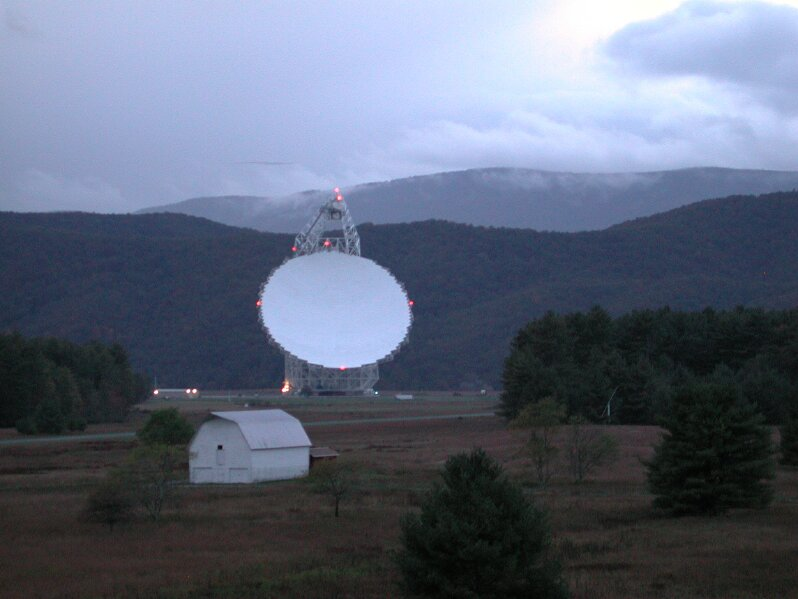
\includegraphics[width=4.5in,bb=0 0 798 599]{GBT.jpg} }
%{\bfseries 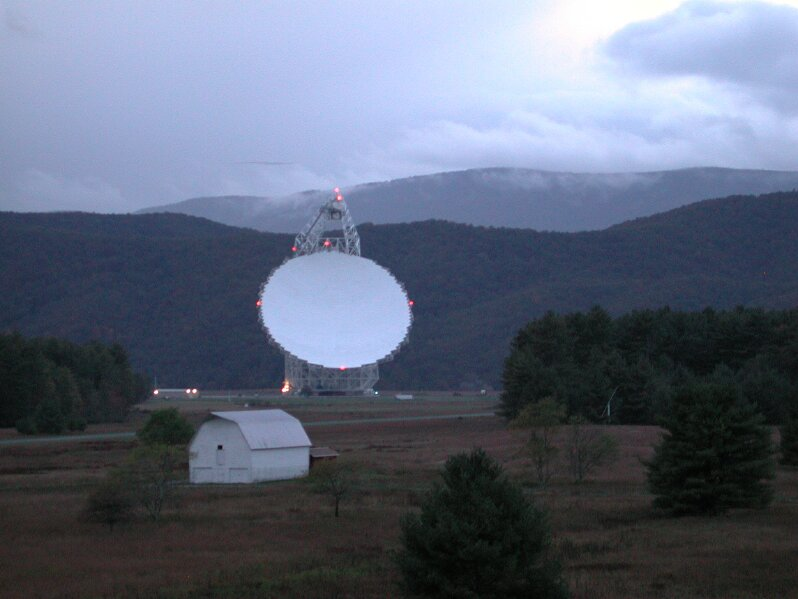
\includegraphics[scale=0.5]{GBT.jpg} }
\end{center}

\vspace*{\stretch{1}}
\begin{center}
{{\LARGE by GBT Scientific Staff\\ \bigskip} \large \today \\ \bigskip Version 4.0}
\end{center}

\vspace*{\stretch{1}}
\begin{center}
{This guide provides essential information for the preparation of
\\ Scheduling Blocks for observations with the Green Bank Telescope.
}
\end{center}
\end{FrameCover}
}

\newpage
\setcounter{page}{0}
%an intentionally added blank page for the back of the cover page
\newpage


% acknowledgements

% \vspace*{\stretch{1}}
\vspace*{2in}

\begin{center}
{{\bigskip \LARGE Authors, Contributors, and Editors\\ \bigskip} 
\large This Guide is the product of many of the GBT Scientific Staff, with major contributions from:\\
\bigskip
\large Dana Balser\\ \bigskip
\large Jim Braatz\\ \bigskip
\large David Frayer\\ \bigskip
\large Frank Ghigo\\ \bigskip
\large Amanda Kepley \\ \bigskip
\large Adam Kobelski\\ \bigskip
\large Karen O'Neil \\ \bigskip
\large Glen Langston \\ \bigskip 
\large Ryan Lynch \\ \bigskip
\large Ron Maddalena\\ \bigskip
\large Brian Mason\\ \bigskip 
\large Toney Minter\\ \bigskip
\large Dan Perera\\ \bigskip
\large Richard Prestage\\ \bigskip
\large Scott Ransom\\ \bigskip  } 
\end{center}

% \newpage
\pagenumbering{roman}
\setcounter{page}{-12}
\pagestyle{plain}

\setcounter{secnumdepth}{4}
\setcounter{tocdepth}{4}
\tableofcontents

\listoffigures
\listoftables
\lstlistoflistings

\newpage
\mainmatter
\pagenumbering{arabic}
%\setcounter{page}{1}
\pagestyle{headings}
\counterwithin{lstlisting}{chapter}

%%%%%%%%%%%%%%%%%%%%       MAIN BODY (start)   %%%%%%%%%%%%%%%%%%%%%%%%%%%%%%%%%%

\chapter{How To Use This Manual}

This document provides the necessary information to be able to perform 
successful observations with the \gls{GBT}.
\begin{itemize}

\item In Chapter~\ref{chap:process} we briefly outline the features of the
\gls{GBT} and the general observing process.

\item in Chapter~\ref{chap:dss} you are introduced to the Dynamic Scheduling
System.

\item In Chapters~\ref{chap:astrid} and ~\ref{chap:datadisplay} we provide an
introduction to the \glsunset{Astrid}\gls{Astrid} observing interface and other
observing applications.

\item In Chapter~\ref{chap:scripts} we provide example \glspl{SB} that can 
be used in \gls{Astrid}.  We also provide detailed descriptions of the contents
of \glspl{SB}.

\item In Chapter~\ref{chap:tactics} we provide information on the strategies
that should be used and advanced techniques for observing with the \gls{GBT}.

\item Later chapters give basics of observing with various specific instruments:
Chapter~\ref{chap:vegas} for spectral line observing with \glsunset{VEGAS}\gls{VEGAS},
Chapter~\ref{chap:GUPPI} for pulsar observing with \glsunset{GUPPI}\gls{GUPPI},
Chapter~\ref{chap:kfpa} for observing with the \glsunset{KFPA}\gls{KFPA},
Chapter~\ref{chap:wband} for observing with the 4mm (68-92~GHz) receiver,
Chapter~\ref{chap:ccb} for continuum observing with the \glsunset{CCB}\gls{CCB},
%Chapter~\ref{chap:mustang} for mapping with the \glsunset{MUSTANG}\gls{MUSTANG} bolometer array,
Chapter~\ref{chap:vlba} for \glsunset{VLBI}\gls{VLBI} observing with the \gls{GBT}, and
Chapter~\ref{chap:radar} for solar system radar with the \gls{GBT}.

\item In Chapter~\ref{chap:rfi} we provide the locations of where to find more 
information about \glsunset{RFI}\gls{RFI}.

\item In Chapter~\ref{chap:weather} is a discussion of the effect of weather
conditions on observing.

\item In Chapters~\ref{chap:computing} and~\ref{chap:remote} we provide
information on computing and remote observing.

\item In Chapter~\ref{chap:travel} we provide information on what happens before
your observations and directions on getting to Green Bank.

\item In Chapter~\ref{chap:after} we provide information on how to take your data 
home with you and where to obtain the \gls{GBT} spectral line data reduction package,
\gls{GBTIDL}.


\item Additional information and special topics are covered in the Appendices.

\end{itemize}

New users should read Chapters~\ref{chap:process},~\ref{chap:dss},
~\ref{chap:astrid},~\ref{chap:datadisplay},~\ref{chap:scripts},~\ref{chap:tactics},
and~\ref{chap:computing} in their entirety.  They should also read the
remaining Chapters as needed.
        %intro
\chapter{The GBT Observing Process}\label{chap:process}

\vspace{-0.5cm}

\section{Overview Of The Green Bank Telescope}

The 100 meter \glsfirst{GBT} is intended to address a very broad range 
of astronomical problems at radio wavelengths and consequently has an
unusual and unique design. Unlike conventional telescopes that have feed
legs projecting over the middle of the surface, the \gls{GBT}'s aperture
is unblocked so that incoming radiation meets the surface directly. This
increases the useful area of the telescope and reduces reflection and
diffraction, which ordinarily complicate a telescope's pattern of response
to the sky. To keep the aperture unblocked, the design incorporates an
off-axis feed arm that cradles the dish and projects upward at one edge.
This requires that the figure of the telescope surface be asymmetrical.
To make a projected circular aperture 100 meters in diameter, the dish is
actually a 100 by 110 meter section of a conventional, rotationally
symmetric 208 meter figure, beginning four meters outward from the
vertex of the hypothetical parent structure (see
Figure~\ref{fig:GBT}). The \gls{GBT}'s lack of circular symmetry
greatly increases the complexity of its design and construction.

\begin{figure}[!h]
\begin{center}
\subfloat[\label{fig:parentparabola}]
{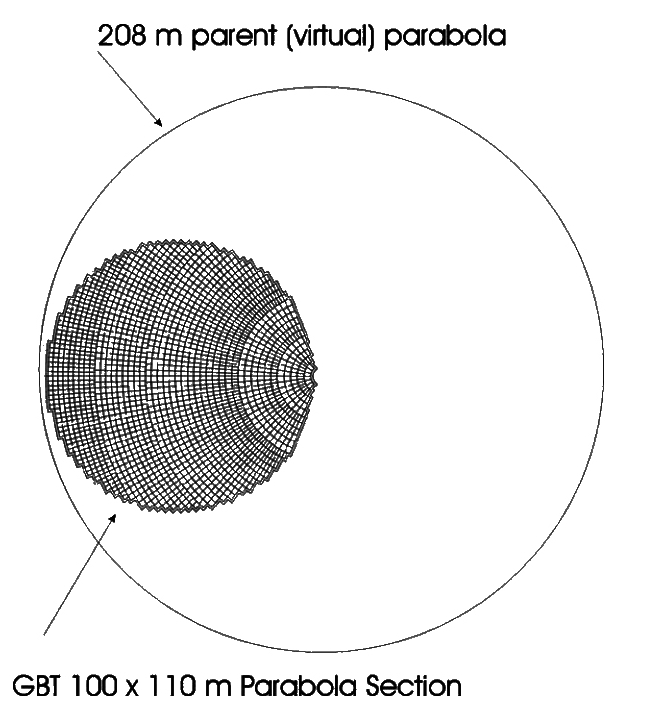
\includegraphics[width=.3\linewidth]{parent-parabola_crop.jpg}}
\hspace{.1\linewidth}
\subfloat[\label{fig:offaxis}]
{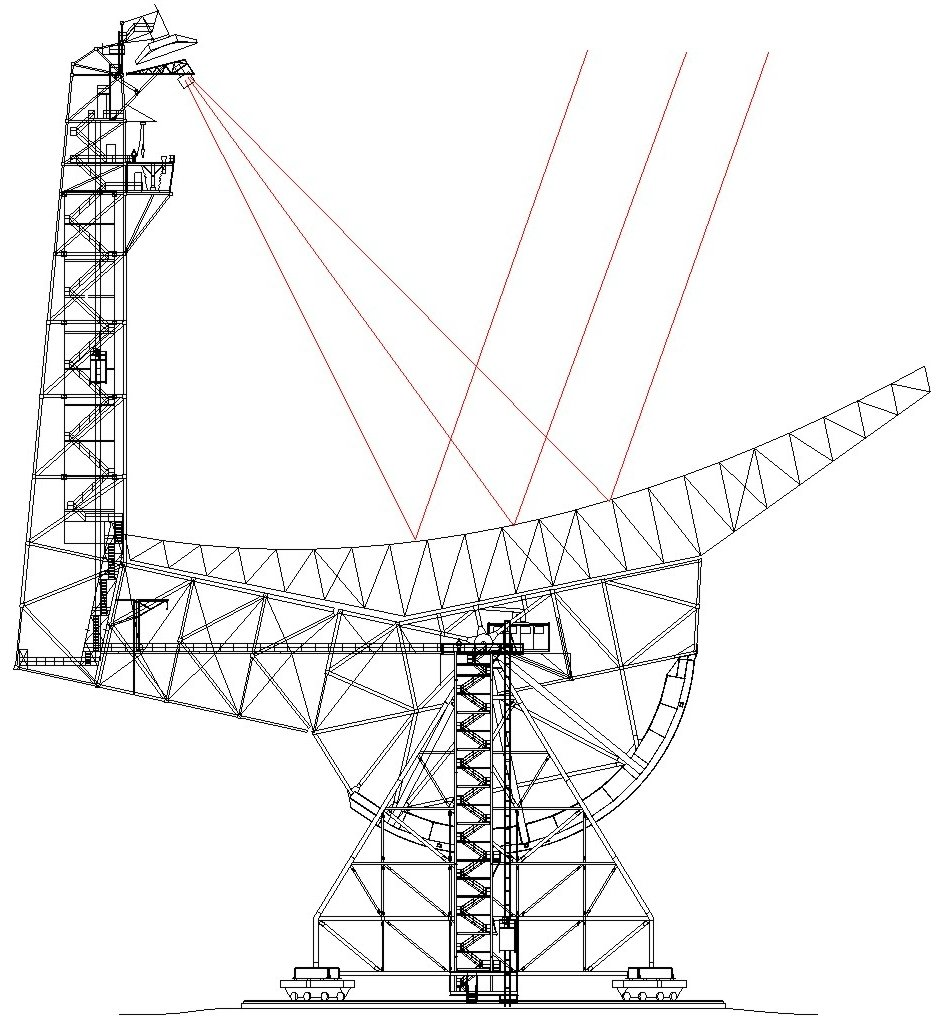
\includegraphics[width=.3\linewidth]{gbt_offaxis_crop.jpg}}
\caption[The parent parabola and off-axis design of the GBT]
{The parent parabola (\ref{fig:parentparabola}) and off-axis design
(\ref{fig:offaxis}) of the \gls{GBT}.\label{fig:GBT}}
\end{center}
\end{figure}

To maintain precise surface figures and pointing accuracy at high frequencies 
the telescope is equipped with a complex \gls{AS}. At higher frequencies
gravity distorts the surface figure of the telescope to unacceptable levels.
Temperature variations and wind can also deform the figure of the dish. To
compensate for these distortions, the surface of the \gls{GBT} is \dq{active}
i.e. it is made up of 2008 independent panels and each of these panels are
mounted on actuators at the corners, which can raise and lower the panels to
adjust the shape of the dish's surface. 

\newpage

\subsection{Main Features of the GBT}


\begin{itemize}[leftmargin=*,itemsep=1pt]
\item {\bf Fully steerable antenna}: +5$^\circ$ to +90$^\circ$ elevation range 
(-46.5$^\circ$ to +90$^\circ$ declination); 85\% coverage of the celestial sphere.  
Note that observing at elevations $>$86$^\circ$ (or 80$^\circ$ during extremely
cold weather) may fail due to the high azimuth rates required.
\item {\bf Unblocked aperture}: Reduces sidelobes, \gls{RFI}, and spectral standing waves.
\item {\bf Active surface}: Compensates for gravitational and thermal distortions.
\item {\bf Frequency coverage of 100 MHz to 115+ GHz}: 3 orders of magnitude of
frequency coverage for maximum scientific flexibility.
\item {\bf Location in the National Radio Quiet Zone}: Comparatively low \gls{RFI}
environment\\ (See Figure~\ref{fig:nrqz}).
\item {\bf Dynamic Scheduling}: Matching scientific programs to the required
weather conditions.
\end{itemize}

\glsunset{NAD83}
\glsunset{NAVD88}

\begin{table}[!h]
\begin{center}
\begin{tabular}{p{.25\linewidth}p{.6\linewidth}}
\toprule
Location & Green Bank, West Virginia, USA \\
\midrule
Coordinates & Longitude: $79\degree 50\arcminute 23.406\arcsecond$ West (\gls{NAD83})\newline
              Latitude: $38\degree 25\arcminute 59.236\arcsecond$ North (\gls{NAD83})\newline
              Track Elevation: 807.43~m (\gls{NAVD88})\\
\midrule
Optics & 110~m $\times$ 100~m unblocked section of a 208~m parent paraboloid Offaxis feed arm\\
\midrule
Telescope Diameter & 	100 m (effective) \\
\midrule
Available Foci & Prime and Gregorian \newline
                 f/D (prime) = 0.29 (referred to 208 m parent parabola) \newline
                 f/D (prime) = 0.6 (referred to 100 m effective parabola) \newline
                 f/D (Gregorian) = 1.9 (referred to 100 m effective aperture) \\
\midrule
Receiver mounts & Prime: Retractable boom with Focus-Rotation Mount \newline
                  Gregorian: Rotating turret with 8 receiver bays \\
\midrule
Subreflector & 	8-m reflector with Stewart Platform (6 degrees of freedom) \\
\midrule
Main reflector & 2004 actuated panels (2209 actuators) \newline
                 Average intra-panel RMS $68~\mu$m \\
\midrule
FWHM Beamwidth & Gregorian Feed: $\sim{ 12.60\arcminute / f_{GHz}}$ \newline
                 Prime Focus: $\sim {13.01\arcminute / f_{GHz}}$ \\
\midrule
Elevation Limits & Lower limit: $5\degree$ \newline
                   Upper limit: $90\degree$ \\
\midrule
Declination Range  & Lower limit: $-46.5\degree$ \newline
                     Upper limit: $90\degree$ \\
\midrule
Slew Rates & Azimuth:	$35.2\degree$/min \newline
             Elevation: $17.6\degree$/min \\
\midrule
Surface RMS & Passive surface: $450~\mu$m at $45\degree$ elevation,
              worse elsewhere \newline
              Active surface: $\sim250~\mu$m, under benign night-time conditions \\
\midrule
Tracking accuracy ($\sigma_{tr}$) & $\sigma_{tr}^2 = \sigma_0^2 + \left(s/3.5\right)^4$ \newline
                                   $\sigma_0$ = night:1.32\arcsecond, day:2.19\arcsecond;
                                   $s$ = wind speed (ms$^{-1}$)\\
\midrule
Pointing accuracy & 5\arcsecond\ blind pointing accuracy \\
\bottomrule
\end{tabular}
\caption{GBT Telescope Specifications.} \label{table:antenna}
\end{center}
\end{table}

\newpage

\subsection{National Radio Quiet Zone}

The \gls{NRQZ} was established by the Federal Communications Commission (FCC)
and by the Interdepartmental Radio Advisory Committee (IRAC) on November 19,
1958 to minimize possible harmful interference to the \gls{NRAO} in Green
Bank, WV and the radio receiving facilities for the United States Navy in
Sugar Grove, WV. The \gls{NRQZ} is bounded by \glsfirst{NAD83} meridians of
longitude at 78d~29m~59.0s~W and 80d~29m~59.2s~W and latitudes of
37d~30m~0.4s~N and 39d~15m~0.4s~N, and encloses a land area of
approximately 13,000 square miles near the state border between Virginia
and West Virginia.\\

\begin{itemize}
\item Further information on the \gls{NRQZ} can be obtained at\\ \vspace{-5mm}
\begin{itemize}
\item \htmladdnormallink
{https://science.nrao.edu/facilities/gbt/interference-protection/nrqz/}
{https://science.nrao.edu/facilities/gbt/interference-protection/nrqz/}
\end{itemize}
\item Information on the West Virginia State Code Chapter 37A
\dq{Radio Astronomy Zoning Act} (WVRAZ) can be found at\\ \vspace{-5mm}
\begin{itemize}
\item \htmladdnormallink
{http://www.legis.state.wv.us/WVcode/code.cfm?chap=37a\&art=1}
{http://www.legis.state.wv.us/WVcode/code.cfm?chap=37a\&art=1}
\end{itemize}
\end{itemize}

\begin{figure}[!h]
\begin{center}
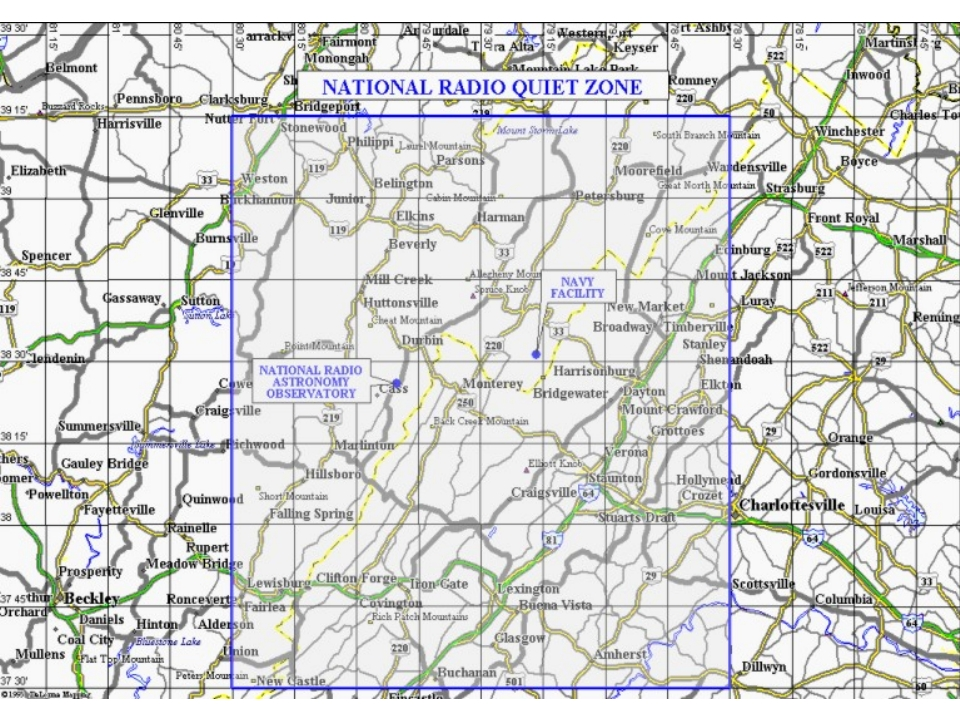
\includegraphics[width=\linewidth]{NRQZ.jpg}
\caption[National Radio Quiet Zone]
{The National Radio Quiet Zone.
\label{fig:nrqz}}
\end{center}
\end{figure}

\newpage


\subsection{Front Ends}

The \gls{GBT} receivers cover several frequency bands from
0.290 - 50 GHz and 70 - 100 GHz. Table~\ref{table:rx} lists the properties
of the Prime Focus receivers and the Gregorian Focus receivers. System temperatures
are derived from lab measurements or from expected receiver performance given
reasonable assumptions about spillover and atmospheric contributions.

The \gls{GBT} Proposer's Guide (\htmladdnormallink
{https://science.nrao.edu/facilities/gbt/proposing/GBTpg.pdf}
{https://science.nrao.edu/facilities/gbt/proposing/GBTpg.pdf}) 
provides more information on the \gls{GBT} receivers.

%\begin{table}[!h]
%\begin{center}
%\caption[Prime Focus receiver properties]{Properties of the Prime Focus 
%Receivers.}\label{table:pfrx}
%\begin{tabular}{llcccccc}
%\toprule
%\multicolumn{2}{c}{Name} & Freq. Range (GHz) & Polarization & Beams & Polns/Beam & 	\gls{Trec} & \gls{Tsys} \\
%\midrule
%\gls{PFone} & Rcvr\_342 & 0.290-0.395 &	Lin/Circ &	1 &	2 &	12 &	46 \\
%\gls{PFone} & Rcvr\_450 & 0.385-0.520 &	Lin/Circ &	1 &	2 &	22 &	43 \\
%\gls{PFone} & Rcvr\_600 & 0.510-0.690 &	Lin/Circ &	1 &	2 &	12 &	22 \\
%\gls{PFone} & Rcvr\_800 & 0.680-0.920 &	Lin/Circ &	1 &	2 &	21 &	29 \\
%\gls{PFtwo} & Rcvr\_1070& 0.910-1.230 &	Lin/Circ &	1 &	2 &	10 &	17 \\
%\bottomrule
%\end{tabular}
%\end{center}
%\end{table}

\begin{table}[!h]
\begin{center}
\caption[GBT receiver properties]
{Properties of the Prime Focus and Gregorian Focus Receivers.}
\label{table:gregrx}
\begin{tabular}{llcccccc}
\toprule
\multicolumn{2}{c}{Name} & $\nu$ Range & Polarization & Beams & Polns/& \gls{Trec} & \gls{Tsys} \\
   &                     & (GHz)       &              &       & Beam  &    (K)     &   (K)      \\
\midrule
\addlinespace
\multicolumn{8}{c}{--- Prime Focus Receivers ---}\\
\addlinespace
%\cmidrule(l{7em}r){2-5}
\gls{PFone} & Rcvr\_342 & 0.290-0.395 &	Lin/Circ &	1 &	2 &	12 &	46 \\
\gls{PFone} & Rcvr\_450 & 0.385-0.520 &	Lin/Circ &	1 &	2 &	22 &	43 \\
\gls{PFone} & Rcvr\_600 & 0.510-0.690 &	Lin/Circ &	1 &	2 &	12 &	22 \\
\gls{PFone} & Rcvr\_800 & 0.680-0.920 &	Lin/Circ &	1 &	2 &	21 &	29 \\
\gls{PFtwo} & Rcvr\_1070& 0.910-1.230 &	Lin/Circ &	1 &	2 &	10 &	17 \\
\addlinespace
\midrule
\addlinespace
\multicolumn{8}{c}{--- Gregorian Focus Receivers ---} \\
\addlinespace
\gls{Lband} & Rcvr1\_2           & 1.15-1.73 & Lin/Circ & 1 & 2 &      6 & 20 \\
\gls{Sband} & Rcvr2\_3           & 1.73-2.60 & Lin/Circ & 1 & 2 &   8-12 & 22 \\
\gls{Cband} & Rcvr4\_6           & 3.95-8.0  & Lin/Circ & 1 & 2 &     5  & 18 \\
\gls{Xband} & Rcvr8\_10          & 8.00-10.1 & Circ     & 1 & 2 &     13 & 27 \\
\gls{Kuband}& Rcvr12\_18         & 12.0-15.4 & Circ     & 2 & 2 &     14 & 30 \\ %\midrule
\gls{KFPA}  & RcvrArray18\_26    & 18.0-26.5 & Circ     & 7 & 2 &  15-25 & 30-45 \\
\gls{Kaband}& Rcvr26\_40 (MM-F1) & 26.0-31.0 & Lin      & 2 & 1 &     20 & 35 \\
\gls{Kaband}& Rcvr26\_40 (MM-F2) & 30.5-37.0 & Lin      & 2 & 1 &     20 & 30 \\
\gls{Kaband}& Rcvr26\_40 (MM-F3) & 36.0-39.5 & Lin      & 2 & 1 &     20 & 45 \\
\gls{Qband} & Rcvr40\_52         & 38.2-49.8 & Circ     & 2 & 2 &  40-70 & 67-134 \\ %\midrule
\gls{Wband} & Rcvr68\_92 (FL1)   & 67-74     & Lin/Circ & 2 & 2 & 50  & 160 \\ 
\gls{Wband} & Rcvr68\_92 (FL2)   & 73-80     & Lin/Circ & 2 & 2 & 50  & 120 \\ 
\gls{Wband} & Rcvr68\_92 (FL3)   & 79-86     & Lin/Circ & 2 & 2 & 50  & 100 \\ 
\gls{Wband} & Rcvr68\_92 (FL4)   & 85-92     & Lin/Circ & 2 & 2 & 60  & 110 \\ 
%MUSTANG & 80-100   &     -     &     64 & - &   -   & - \\
\bottomrule
\end{tabular}
\end{center}
\end{table}

\subsubsection{Prime focus receivers}

The Prime focus receivers are mounted in a \gls{FRM} on a retractable boom.
The boom is moved to the prime focus position when prime focus receivers are
to be used, and retracted when using Gregorian receivers. The \gls{FRM} holds
one receiver box at a time.  Currently there are two receiver boxes, \gls{PFone}
and \gls{PFtwo}.  A change from \gls{PFone} to \gls{PFtwo} receivers requires
a box change, taking about 4 hours and done only during scheduled maintenance days. 

The \gls{PFone} (0.29 - 0.92~GHz) receiver is divided into 4 frequency bands
within the same receiver box. The receivers are cooled \gls{FET} amplifiers.
The feeds for the lower three bands are short-backfire dipoles, and the feed
for the fourth (680-920MHz) is a corrugated feed horn with an \gls{OMT} polarization
splitter. A feed change, required to switch between bands, takes 4 hours and
must occur on a maintenance day. The \gls{PFtwo} (0.920 - 1.23~GHz) receiver 
uses a cooled \gls{FET} and a corrugated feed horn with the \gls{OMT}.

\newpage

\subsubsection{Gregorian focus receivers}

The Gregorian receivers are mounted in a rotating turret in a receiver room 
located at the Gregorian Focus of the telescope. The turret has 8 portals for 
receiver boxes. Up to 8 receivers can be kept cold and active at all times. 
Changing between any two Gregorian receivers that are installed in the turret
takes about 60-90 seconds.

%\subsubsection{The MUSTANG Receiver}
%\glsfirst{MUSTANG} is a multi-pixel bolometer array observing at 80-100 GHz
%mounted at the Gregorian focus.  It is both a receiver and the associated
%back end, and is described in Chapter~\ref{chap:mustang}. The \gls{MUSTANG}
%receiver must be used at elevations above 30\degree, due to the design of
%the cryogenics.


\subsection{Backends}\label{sec:backends}

The \gls{GBT} has two continuum backends: the \gls{DCR} and the \gls{CCB}.
The spectral line backend is \gls{VEGAS}.  Pulsar observations can be done
with \gls{GUPPI}.  There is a single dish mode for the \gls{VLBA} backend
that is available for high time--resolution observations.  Planetary radar
uses a specialized backend.

For more information on \gls{GBT} backends, please see the \dq{\gls{GBT}
Proposer's Guide} which is available at \htmladdnormallink
{http://www.gb.nrao.edu/gbtprops/man/GBTpg/GBTpg\_tf.html}
{http://www.gb.nrao.edu/gbtprops/man/GBTpg/GBTpg_tf.html}.

\subsubsection{Digital Continuum Receiver (DCR)}

The \gls{DCR} is the \gls{GBT}'s general purpose continuum backend.
It is used both for utility observations such as pointing, focus,
and beam-map calibrations, as well such as for continuum astronomical
observations including point-source on/offs, extended source mapping, etc.


\subsubsection{Caltech Continuum Backend (CCB)}

The \gls{CCB} is a sensitive, wideband backend designed exclusively for use
with the \gls{GBT} \gls{Kaband} (26-40~GHz) receiver. It provides a carefully
optimized \gls{RF} (not an \gls{IF}) detector circuits and the capability to
beam-switch the receiver rapidly to suppress instrumental gain fluctuations. 
There are 16 input ports (only 8 can be used at present with the \gls{Kaband}
receiver), hard-wired to the receiver's 2 feeds $\times$ 2 polarizations
$\times$ 4 frequency sub-bands (26-29.5 , 29.5-33.0; 33.0-36.5; and 36.5-40~GHz).
The \gls{CCB} allows the left and right noise-diodes to be controlled individually
to allow for differential or total power calibration. Unlike other \gls{GBT}
backends, the noise-diodes are either on or off for an entire integration (there
is no concept of \dq{phase within an integration}). The minimum practical
integration period is 5 milliseconds; integration periods longer than 0.1 seconds
are not recommended. The maximum practical beam-switching rate is about 4 kHz,
limited by the needed $250\mu s$ beam-switch blanking time. Switching slower
than 1 kHz is not recommended.

\subsubsection{VEGAS}

\glsfirst{VEGAS} is the spectral line backend for the \gls{GBT}. It consists of
eight independent dual polarization spectrometers (banks) that can be configured in
any one of 29 modes and can be used with any receiver except \gls{MUSTANG}. It
provides up to 64 spectral windows as well as wide bandwidths (1000-1500~MHz).
See chapter~\ref{chap:vegas} for detailed information on \gls{VEGAS}.


\subsubsection{GUPPI}

\glsfirst{GUPPI} has one hardware mode and many software modes.  \gls{GUPPI}
can be used with any receiver with the exception of \gls{MUSTANG}.  Only one
polarization would be available for the \gls{Kaband} (26-40~GHz) receiver.
\gls{GUPPI} uses 8-bit sampling to dramatically improve dynamic range and
\gls{RFI} resistance.  Currently \gls{GUPPI} can use bandwidths of 100, 200
and 800 MHz with 2 polarizations and full stokes parameters.  The minimum
integration time is $40.96\mu s$ using 2048 channels and an 800 MHz bandwidth.
See the introduction to \gls{GUPPI} in Chapter~\ref{chap:GUPPI}.


%\subsubsection{MUSTANG}
%
%See the introduction to \gls{MUSTANG} in Chapter~\ref{chap:mustang}.

\subsubsection{\dq{VLBI}}

The \gls{GBT} supports \glsfirst{VLB} observations with a Mark5 \gls{VLBA}
recorder. This recorder can also be used in a \dq{single-dish} mode to make
high time--resolution observations.  See Chapter~\ref{chap:vlba} for more
information.

\subsubsection{Radar}
Planetary radar observations are supported by the \glsfirst{PFS} and
JPL radar backends.  See Chapter~\ref{chap:radar} for more information.

\subsection{Polarization Measurements}

Measurement of Polarization and Stokes parameters is possible using
\gls{VEGAS} and \gls{GUPPI}.  This is an \dq{expert user} mode: users should
contact their GBT support person or the GBT helpdesk.  For an introduction to
polarization observations, see \dq{A Heuristic Introduction to
Radioastronomical Polarization}, by C. Heiles, ASP Conference Series
Vol 278, 2002.

\newpage

\section{The GBT Observing Process}

The following list summarizes the general flow of how \gls{GBT} observing
proceeds. By the time you are reading this document you should have already
been through several of the steps.

\begin{description}[leftmargin=*]
\item[Step 1 - Contact your GBT \dq{friend}]\ \\
Before you observe, you need to prepare for your observations
(see Chapter~\ref{chap:travel}) and set up your computing account
(see Chapter~\ref{chap:computing}). You will be assigned a scientific
contact person (\gls{GBT} \dq{friend}) whom you should contact well in
advance of your observing to determine optimum dates for a visit and ensure
the telescope and hardware will be available for the project while you are
on site. Your \dq{friend} will help you develop a appropriate observing tactics
for your proposal (see Chapter~\ref{chap:tactics}). They will also help you
with any technical questions e.g., dealing with \gls{RFI} (see
Chapter~\ref{chap:rfi}), etc. At this time you should review your project
page(s) in the \glsfirst{DSS} (see Chapter~\ref{chap:dss}) and develop your
\glsfirstplural{SB} (see Chapter~\ref{chap:scripts}).

\item [Step 2 - Make travel arrangements]\ \\
If you are an experienced \gls{GBT} observer, you can observe remotely
(see Chapter~\ref{chap:remote}). If you are new to the \gls{GBT}, you
must plan to travel to Green Bank (see Chapter~\ref{chap:travel}) and
spend at least a week and preferably two weeks at the site to ensure
appropriate weather conditions for the observations (see
Chapter~\ref{chap:weather}). You should arrive in Green Bank at least
one business day before your observations. This will allow you to meet
with the contact scientist and also with the scientific staff person who
will be \dq{on call} during your observations (these might be different people).
After hands-on experience with observing you will qualify for remote observing.

\item [Step 3 - Set blackout dates in the DSS]\ \\
If there are periods of time or dates when you cannot observe, you should
indicate these as \dq{blackout dates} in the \gls{DSS} web page
\htmladdnormallink{https://dss.gb.nrao.edu}{https://dss.gb.nrao.edu}.
Those visiting Green Bank should use blackout dates to mark the periods of
their travel before and after their stay to ensure they are scheduled only
when available and ready.

\item [Step 4 - Wait for scheduling notification]\ \\
Unless you are running a project which must be fixed to a certain date and
time, your observations will be dynamically scheduled.  See
Chapter~\ref{chap:dss} for details on how dynamical scheduling is done with
the \gls{GBT}. When your project is scheduled you will receive an e-mail
notification indicating the exact time the observing session will start.
Notifications go to the project PI and all others designated as observers
on the project.  Thus you should have prepared your scripts and be ready
to observe with 24-36 hours notice.  

\item [Step 5 - 30 minutes before your observation session]\ \\
If you are present in Green Bank, go to the control room and log into
one of the computers.  Bring up any programs that you need so that you are
prepared when your observation time begins.

If you are observing remotely (see Chapter~\ref{chap:remote}) you should
contact the \gls{GBT} operator through \textit{talk and draw}
(see~\ref{sec:talkanddraw}) or call on 304-456-2341 or 304-456-2346.  In case
of a site phone or power outage, the direct line to the control room is
304-456-3203. You should give the operator your contact information (phone
numbers, emails) so that they can contact you during the observations
if necessary.  You will also need to let the operator know what computer
you will be using during your observations.  At this time you will begin
to open a \gls{VNC} session that you will use for the remote observations.
Starting this early will allow for any problems encountered while preparing
to observe remotely to be solved before the observations are to begin.
\vspace{-5mm}
\begin{itemize}[leftmargin=*,itemsep=0pt]
\item You can find information about \gls{GBT} remote observing policies at\\
\vspace{-5mm}
\begin{itemize}[itemsep=0pt]
\item \htmladdnormallink
{https://science.nrao.edu/facilities/gbt/observing/policies}
{https://science.nrao.edu/facilities/gbt/observing/policies}
\end{itemize}
\item You can find information about opening a \gls{VNC} session at\\
\vspace{-5mm}
\begin{itemize}[itemsep=0pt]
\item \htmladdnormallink
{https://science.nrao.edu/facilities/gbt/observing/remote-observing-with-the-gbt}
{https://science.nrao.edu/facilities/gbt/observing/remote-observing-with-the-gbt}.
\end{itemize}
\end{itemize}

\newpage

\item [Step 6 - Operator responsibilities]\ \\
The operator on duty will handle several tasks for you at the beginning of
your observations.  They will \dq{put you in the gateway} (give you security
access) so that you can control the \gls{GBT}.  They will also get the correct
receiver into the focus position of the \gls{GBT}, get the antenna motor drives
ready for movement, place the correct pointing models into the system, and set
the \gls{GBT}'s \glsfirst{AS} into the proper state.  The operator is there
to take care of all safety issues concerning the \gls{GBT}.

\item [Step 7 - Begin observations]\ \\
Now you are ready to observe.  You will use the \gls{Astrid} (see
Chapter~\ref{chap:astrid}) to perform your observations by submitting an
\gls{SB} (see Chapter~\ref{chap:scripts}).  The steps you will take in
observing are generally:
\begin{enumerate}[leftmargin=*,label={\bf \Alph*}]
\item Configure the hardware to the desired states. The parameters used
to determine these states are known as the \dq{configuration} and the
act of setting these states is known as \dq{configuring}.
\item Slew to your source.
\item Balance the \gls{IFsys}. In this step you command the system to
automatically adjust amplifier and attenuator settings in the \gls{IFsys} to
ensure that all components operate within their linear regime.
\item Execute your observations using one of the \gls{SB} Scan Types
(see Chapter~\ref{chap:scripts}).
\item If problems develop let the operator know and they will either help
solve the issue or contact the on-call support scientist for assistance. 
\end{enumerate}

\item [Step 8 - Immediately after observations]\ \\
Once you are done observing you should close \gls{Astrid}, log out of
the computer you were using, and leave the control room.  Or, if
observing remotely, {\bf properly close your \gls{VNC} session} using the
{\tt vncserver -kill} command.

\item [Step 9 - Data reduction]\ \\
During and after your observing run you will reduce your data. You will generally
use \gls{GBTIDL} for data reduction of spectral line data.  This can be done
either at Green Bank or your home institution.  Continuum reduction support is
available for the \gls{CCB} (see Chapter~\ref{chap:ccb}).  Otherwise only rudimentary continuum data reduction
support is available for the \gls{GBT} at this time, and you should contact
your \gls{GBT} \dq{friend} for more information. A pulsar data reduction
package, \glsunset{PRESTO}\gls{PRESTO}, is available from Scott Ransom.

Use one of the data reduction machines, not the workstations used for running
the observations.  Refer to \htmladdnormallink
{http://www.gb.nrao.edu/pubcomputing/data-reduction.shtml}
{http://www.gb.nrao.edu/pubcomputing/data-reduction.shtml}
for a list of data reduction machines at Green Bank.

Note that observers wishing to reduce VEGAS data will need access to the
\dq{lustre} file system.  Refer to
\htmladdnormallink{http://www.gb.nrao.edu/pubcomputing/public.shtml}
{http://www.gb.nrao.edu/pubcomputing/public.shtml} for a list of lustre clients.

\item [Step 10 - Transfer your data]\ \\
Once you are done you will want to transfer your data to your home institution
(see Chapter~\ref{chap:after}).

\item [Step 11 - Keep in touch]\ \\
Finally you will want to write your Nobel Prize winning paper. The \gls{NRAO} can
help you with your page charges (see Chapter~\ref{chap:after}). You should also
notify your scientific contact person of your paper to help the Observatory
keep track of how successful all observing projects have been.

\end{description}



%%%%%%%%%% END CHAPTER.... % the GBT observing process
\chapter{Introduction to the Dynamic Scheduling System}\label{chap:dss}
This chapter gives an introduction to the \glsfirst{DSS} for the Robert C.
Byrd Green Bank Telescope (\gls{GBT}). The \gls{GBT} has been scheduled with the
\gls{DSS} since October 1, 2009. Observers can access the \gls{DSS} through this site:
\htmladdnormallink{https://dss.gb.nrao.edu}{https://dss.gb.nrao.edu}

%%%%%%%%%%%%%%%%%%%%%%%%%%%%%%%%%%%%%%%%%%%%%%%%%%%%%%%%%%%%%%%%%%%%%%%%%%%%%%
\section{Overview of the DSS}
The primary goal of the Green Bank Telescope \glsfirst{DSS} is to improve the
efficiency of \gls{GBT} observations by matching the observing schedule to
predicted weather conditions while allowing each observer to retain interactive
control of the telescope. Each day the \gls{DSS} will examine the weather forecast,
equipment availability, observer availability, and other factors, and set an
observing schedule for the 24-hour period beginning the next day. Observers will
therefore get about 24-48 hours notice before their project will observe.
Observers will have the opportunity to suspend their observing program, set
blackout dates indicating when they are unavailable for observing, and back out of
current observations if they find the observing conditions are not suitable to
their science goals.

The \gls{DSS} readily accommodates remote observing, but by being on site in
Green Bank observers increase their likelihood of being scheduled during the
period of their visit. Visits to Green Bank should be arranged in advance with
the project's \dq{Friend}, and observers should ideally spend one to two weeks
in Green Bank to give enough opportunity for their project to get scheduled at
least once. {\bf Projects observing at high frequencies (20 GHz and higher)
typically require staying in Green Bank for two weeks or longer.}



%%%%%%%%%%%%%%%%%%%%%%%%%%%%%%%%%%%%%%%%%%%%%%%%%%%%%%%%%%%%%%%%%%%%%%%%%%%%%%
\section{DSS Terminology}

The process of scheduling \gls{GBT} observations begins with the preparation of
the proposal using the \gls{NRAO} Proposal Submission Tool (PST). Proposals accepted
by the \gls{NRAO} Time Allocation Committee become \gls{GBT} projects that appear
in the \gls{DSS} system and are identified by an assigned project ID
(e.g., GBT09A-001).

Projects are divided into sessions, which have associated parameters that define how 
the observation should be scheduled. These parameters include sky position, time
allocated, observing frequency, and minimum and maximum durations preferred for a
single, contiguous block. Sessions for monitoring observations have additional
parameters describing how often to repeat the observation. The project investigators
initially define the session parameters in the proposal, but the parameters may be
modified by request to the helpdesk (helpdesk-gb@nrao.edu). Observers can see the
most critical session parameters on the \gls{DSS} web pages.

Completing the observations for a session may require scheduling multiple segments.
Each contiguous block of scheduled time is called a {\it telescope period}.

As telescope periods are completed, the project and associated sessions will be
billed for the time. If any time is lost to weather or an equipment failure, the
observer may consult with the telescope scheduler (via the helpdesk) and request
that the project not be billed for the lost time.

%%%%%%%%%%%%%%%%%%%%%%%%%%%%%%%%%%%%%%%%%%%%%%%%%%%%%%%%%%%%%%%%%%%%%%%%%%%%%%
\section{Controlling the Scheduling of a Project}

Users can access their \gls{DSS} account by logging in to the system at 
\htmladdnormallink{https://dss.gb.nrao.edu}{https://dss.gb.nrao.edu}.
The \gls{DSS} username and password are the same as those used for \gls{NRAO}
Interactive Services (i.e., the Proposal Submission Tool).

From the \gls{DSS} web site, users can view and manage the scheduling information
for their projects.  In order for a project session to enter the pool of sessions
eligible for scheduling, the user is responsible for ensuring that the session is
enabled in the \gls{DSS}, and that a qualified observer is available to perform the
observation. Sessions and observers are enabled for observing simply by clicking a
check box in the \gls{DSS} project page (See figure~\ref{fig:dss_project_page}).
Users can control when their project is scheduled by enabling or disabling
individual sessions.

Note that astronomers intending to observe remotely must be trained and approved by
GB staff before the project can be authorized and made eligible for scheduling.

Observers can enter personal blackout dates. Blackouts can be entered either as one time
events (e.g., May 1, 20:00 to May 4, 05:00 UT) or as repeating events (e.g., every
Monday from 15:30 to 17:30 ET). If all observers for a given project are blacked out at a
given time, that project will not get scheduled. If at least one observer is not blacked out,
the project is eligible for scheduling. The default time zone used for entering blackouts is
set on the {\it Preferences} tab, which is linked at the top of every \gls{DSS} web page. Observers
can also override the default by selecting a time zone when making a blackout entry.
Observers with more than one project will find that they need to enter blackout dates only
once, and the dates will be applied to all their projects. {\bf Those visiting Green Bank to
observe should use blackout dates to mark the periods of their travel before and after the
run to ensure they are scheduled only when available and ready on-site.}

{\it Guidelines for the use of blackouts:} While blackout dates give observers control of the
scheduling process, efficient \gls{GBT} operation requires that not too much time be blacked
out or disabled. It is especially important that projects with large observing allocations
not have too much time unavailable for scheduling because of blackouts. As a guideline,
projects with more than 20 hours of allocated observing should limit time that cannot be
scheduled to no more than 20\% of the total eligible observing time over the course of a
semester. If a project cannot meet this guideline, the \glsunset{PI}\gls{PI} is encouraged
to increase observing opportunities by enlisting additional observers who are qualified for
remote observing. Projects that require observers to visit Green Bank for training are excluded
from this guideline until the observers are trained for remote observing.

{\it Caution Regarding Blackouts:} If a project has only one observer, that observer should be
particularly conscientious of blackouts. It can be easy for an observer to inadvertently
hamper observing opportunities by setting blackout dates too freely,
particularly repeating blackouts. Repeating blackouts should be used with care.
Targets with low declinations, such as the Galactic Center, have tightly constrained
observing opportunities to begin with, so observers on such projects
should be particularly careful with blackouts that would further limit their observing
opportunities. Consider, as an example, a project that has a session with a 4-hour
minimum duration to observe the Galactic Center. If the observer has a repeating 1-hour
blackout date that intersects the window, the entire session becomes ineligible each time
the blackout intersects the 4-hour window.  The Green Bank Observatory is not responsible
for lost observing opportunities due to excessive blackouts.

When entering blackouts, keep in mind, too, that projects do expire, so it is in the interest
of the observer to keep the projects eligible for scheduling as much as possible.

%%%%%%%%%%%%%%%%%%%%%%%%%%%%%%%%%%%%%%%%%%%%%%%%%%%%%%%%%%%%%%%%%%%%%%%%%%%%%%
\section{Canonical Target Positions}

The \gls{DSS} keeps track of a project's scheduling requirements via the session parameters,
which can be viewed on the project page. The \gls{PI} should check that session parameters
properly reflect the needs of the project. The project Friend assigned by NRAO can also
offer advice on optimizing session parameters, where appropriate. In some cases, a
session's target position may be representative of a group of objects clustered on the sky.
As the project progresses and some of these targets are observed, this representative
position may need to be updated. In this case, the \gls{PI} should send an email request to
the \gls{DSS} helpdesk.

The \gls{DSS} can automatically update the sky coordinates of common, fast-moving solar
system objects, including comets. The position is updated each day prior to scheduling.
On the project page under {\it Project Sessions}, an asterisk next to the coordinates indicates
that the position for that session is automatically updated in this manner.

Many observers find it helpful to use a sky-plotting tool to help plan their observations
and keep track of target locations on the sky. The \gls{CLEO} Scheduler \& Skyview tool, which
runs on Linux systems in Green Bank and can be run remotely through \gls{VNC}, is one such tool
that allows a \gls{GBT} user to plot target locations on the sky for any date and time. This
application can read target coordinates from a standard astrid catalog file. Observers will find
this tool handy for identifying the time of day a project may get scheduled, as well as helping to
plan observations in detail after they are scheduled. To run the program, type {\tt cleo scheduler}
from the command line. See \S~\ref{sec:cleo_scheduler} for further details on the \gls{CLEO}
Scheduler \& Skyview application.

%%%%%%%%%%%%%%%%%%%%%%%%%%%%%%%%%%%%%%%%%%%%%%%%%%%%%%%%%%%%%%%%%%%%%%%%%%%%%%
\section{Contact Information and Project Notes}

Observers can specify how they should be contacted, prior to and during their
observations. It is critical to keep contact information current.
Each observer can provide {\it dynamic contact} information in a free-format
text box. Here the observer should provide 
any contact information not available through the person's (static) \gls{NRAO}
contact information, which is also listed on the page. Observers can also specify
the order in which they should be contacted by \gls{GBT} operations, in the event
of any schedule changes or in case there is need to contact the observer for any
reason prior to the scheduled start time. Specify the order by clicking the arrow
icons next to the list of team members, on the \gls{DSS} project page.

Finally, observers can record {\it Project Notes} on the \gls{DSS} project web page.
Project notes provide observers a place to store and share observing instructions.
The notes are visible to all project team members as well as the \gls{GBT} operations
staff and schedulers. Observers who need to share instructions or other information
with the \gls{GBT} operator prior to the start of an observation can provide these
instructions in the project notes area. Project notes are not intended to be a log
for observations, but rather a place to store brief instructions or news that should
be shared among observers and the \gls{GBT} operator.

\newpage

\section{The DSS Software}

\subsection{The DSS Home Page}
\begin{figure}[!h]
\begin{center}
\frame{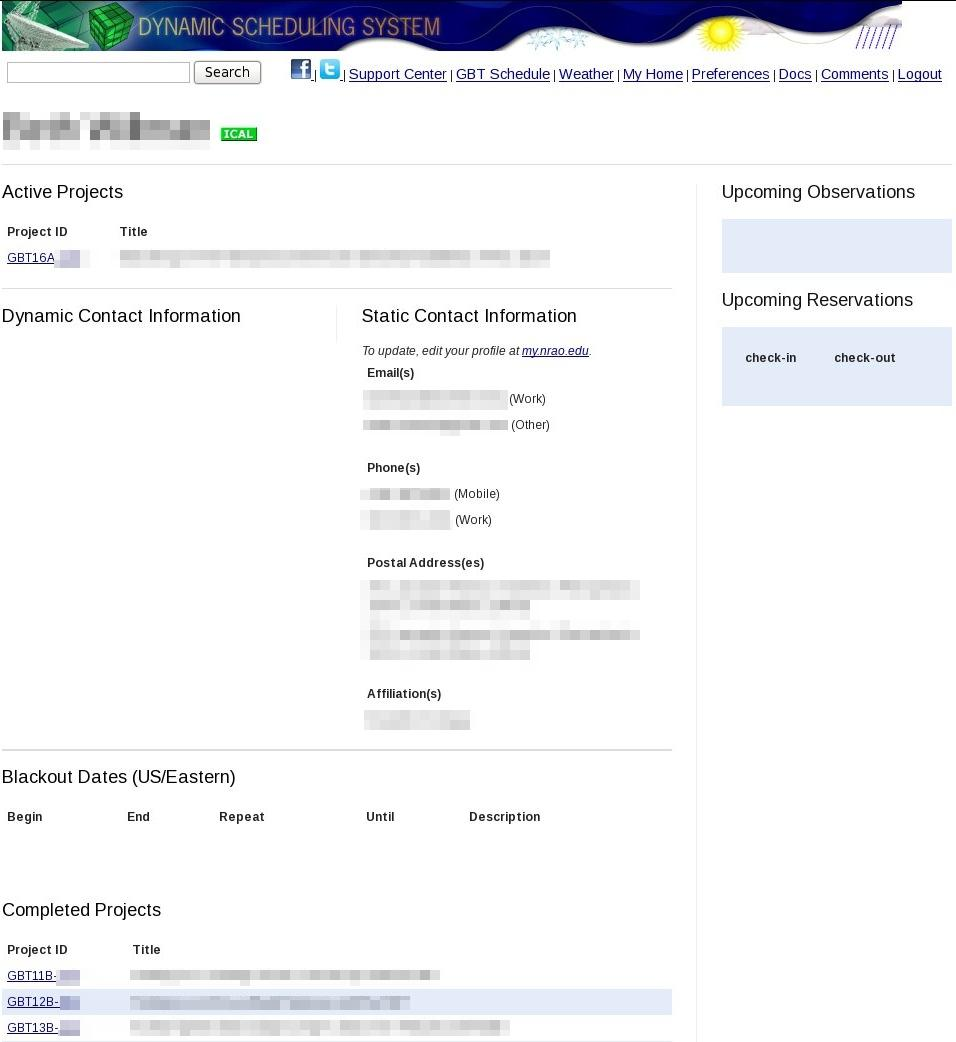
\includegraphics[width=0.6\linewidth]{dss_home_page.jpg}}
\caption[A sample DSS home page]
{A sample \gls{DSS} home page.
\label{fig:dsshome}}
\end{center}
\end{figure}

Upon logging in to the \gls{DSS} system, users arrive at their \gls{DSS} home page
(Figure~\ref{fig:dsshome}) where they see a list of active projects on which they
appear as co-investigator. From the \gls{DSS} home page, users can:
\begin{itemize}[itemsep=1pt]
\item Access the project page for each of their affiliated projects
\item See a list of upcoming observations
\item See a list of upcoming Green Bank room reservations
\item See their {\it static} contact information, as entered in the \gls{NRAO}
      services system \htmladdnormallink{http://my.nrao.edu}{http://my.nrao.edu}.
\item Set {\it dynamic} contact information
\item Set blackout dates
\item Follow a link to the current \gls{GBT} fixed schedule
\item Follow a link to the weather forecasts page
\item follow a link to the \gls{NRAO} support center
\item Set the default time zone via the Preferences link
\item Access \gls{DSS} documentation
\item Establish an iCalendar subscription. Instructions for using iCalendar are available
by hovering the mouse cursor over the iCal icon on the \gls{DSS} Home Page.
\end{itemize}

\newpage

\subsection{The DSS Project Page}

By selecting a project ID, observers are presented with the project page,
where they can:

\noindent\begin{minipage}{0.6\linewidth}
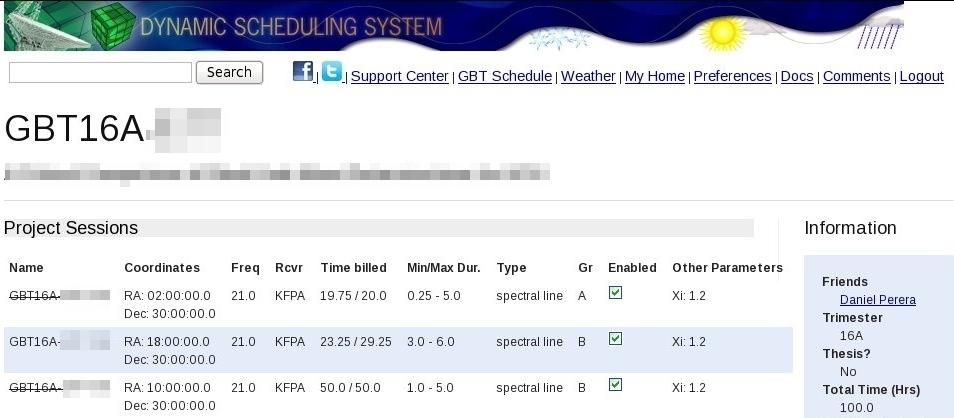
\includegraphics[width=\linewidth]{dss_project_page1.jpg}
\end{minipage}\hfill
\begin{minipage}{0.385\linewidth}
\begin{itemize}[leftmargin=*]
\vspace{2cm}
\item Inspect session parameters
\item Enable or disable individual session
\item View total allocated and billed time
\end{itemize}
\end{minipage}

\noindent\begin{minipage}{0.6\linewidth}
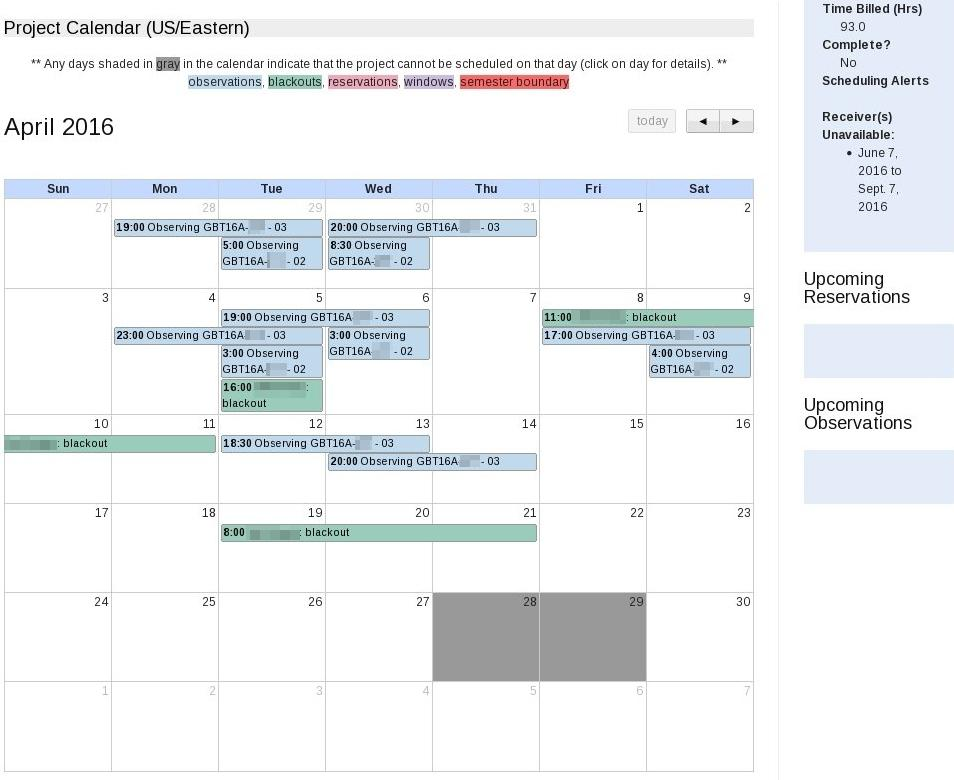
\includegraphics[width=\linewidth]{dss_project_page2.jpg}
\end{minipage}\hfill
\begin{minipage}{0.385\linewidth}
\begin{itemize}[leftmargin=*]
\item See a project calendar
\item View scheduling alerts
\vspace{1.5mm}
\item View receiver availability  %cos minipage is stoopid - or me
\vspace{9mm}
\item View upcoming reservations
\vspace{5mm}
\item View upcoming observations
\vspace{2.8cm}

\end{itemize}
\end{minipage}

\noindent\begin{minipage}{0.6\linewidth}
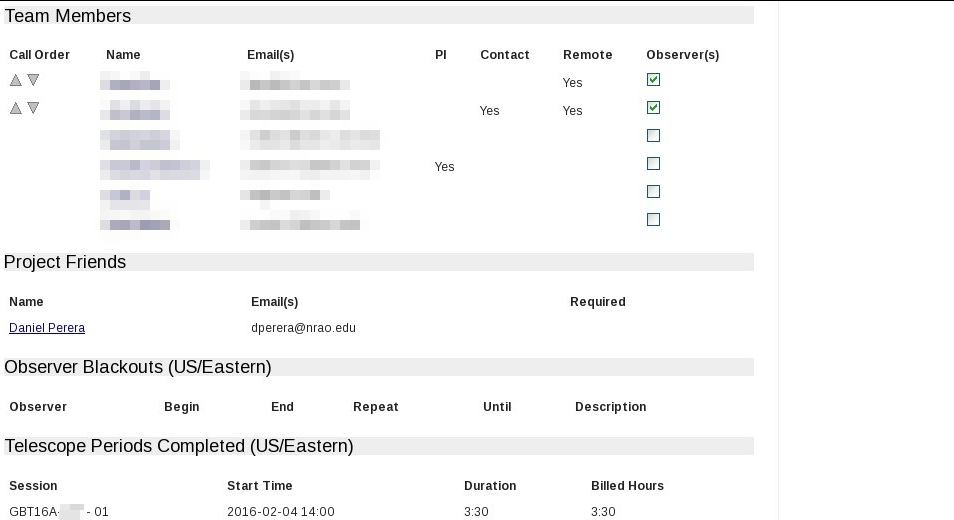
\includegraphics[width=\linewidth]{dss_project_page3.jpg}
\end{minipage}\hfill
\begin{minipage}{0.385\linewidth}
\begin{itemize}[leftmargin=*,itemsep=0pt]
\vspace{5mm}
\item Specify observers from the project team, and set the order they should
      be contacted by \gls{GBT} operations
\vspace{1.3cm}
\item See a list of blackout dates for all\newline observers on the project
\item See a list of completed telescope\newline periods
\end{itemize}
\end{minipage}

\noindent\begin{minipage}{0.6\linewidth}
\setlength{\abovecaptionskip}{-5pt}

\includegraphics[width=\linewidth]{dss_project_page4.jpg}
\captionof{figure}[A sample DSS project page]{A sample DSS project page.}
\label{fig:dss_project_page}
\end{minipage}\hfill
\begin{minipage}{0.385\linewidth}
\begin{itemize}[leftmargin=*]
\item Store and share project notes
\item View your abstract and disposition
\vspace{2.5cm}
\end{itemize}
\end{minipage}

\newpage


The project calendar gives observers an idea when their project is eligible for scheduling.
Regardless of the weather, there will be times when a project is not eligible for
scheduling, for example because of no receiver availability, observer blackouts, fixed
telescope maintenance periods, and other fixed projects appearing on the \gls{GBT} schedule.
Times not eligible for scheduling will be grayed out on the project calendar.

The project calendar helps with planning in a number of ways. However, it is important
to understand that a session's eligibility is based on ever-changing constraints, and
can change from {\it not eligible} to {\it eligible} at any time. Therefore, if
observers wish to take a break from observing based on the calendar outlook, they
should either disable all sessions until they are ready to resume with the observing,
or enter blackout dates to cover the period they do not wish to observe.

The project page includes a panel with project team members listed. Using a checkbox,
team members can select or deselect those identified as observers. They can also
rearrange the order observers are listed. The top observer in the list is expected to
observe the next scheduled session. If there is a change in schedule, this person will be
called first.

\section{Responsibilities}

Each project has a \glsfirst{PI} and, optionally, a list of additional
investigators. An investigator is eligible to be an observer for a given project if
that person is qualified for remote observing or is on site in Green Bank.

It is essential that one of the observers for a scheduled project contact \gls{GBT}
operations at least 30 minutes prior to the start of the observation. Observers can
contact the \gls{GBT} operator by telephone (304-456-2341), by the \gls{CLEO} chat
program \dq{Talk and Draw}  (for qualified remote observers), or by showing up in
the \gls{GBT} control room. If the \gls{GBT} operator has not been contacted before
the session's start time, the operator will phone observers in the order they are
listed on their project web page.

\begin{itemize}[leftmargin=*]
\item The \gls{PI} is responsible for:\\
\vspace{-5mm}
\begin{itemize}[itemsep=1pt]
\item Managing the project
\item Identifying all associated observers
\item Working with project team members and the \gls{GBT} project Friend to ensure that
\glspl{SB} are properly and promptly prepared.
\item Enabling each session by clicking the \dq{enable} button on the project's web page.
Sessions should be enabled only if they will be ready for observing in the next 24 hours.
\item Ensuring that all associated observers have provided contact information,
including a current telephone number and an email address for each observer.
\item Ensuring that a project's scheduling information is current. This includes
checking the hours remaining on the project and ensuring that the session
parameters are up-to-date and accurate.
\item Ensuring that each scheduled telescope period has an observer who is available at
least 30 minutes before the session is scheduled to begin.
\end{itemize}
\item Observers are responsible for:\\
\vspace{-5mm}
\begin{itemize}[itemsep=1pt]
\item Ensuring that the \gls{DSS} project web page has their current contact information. For
remote observers, this includes entering telephone numbers where they can be
reached at the time of observation.
\item Contacting \gls{GBT} operations 30 minutes prior to the start time of an observation.
\item Attending to observations during a scheduled telescope period.  The \gls{PI} is responsible
for \dq{no-shows} and the ensuing reduction in their alloted time. 
\item Notifying \gls{GBT} operations if they find conditions unsuitable for their session.
\end{itemize}
\end{itemize}

\section{Remote Observing }

% The policies and instructions relating to remote observing remain the same. 
To use the \gls{GBT} remotely, observers must first be trained and certified by Green
Bank staff. In general, astronomers must observe at least once in Green Bank before
being certified for remote observing. {\bf Please note that students should be trained
on site by \gls{GBT} staff, not off site by others}. Experienced observers, when using instruments
or observing modes unfamiliar to them, should plan to visit Green Bank if they require
assistance. 

Contact your project \dq{friend} or the \gls{DSS} helpdesk (helpdesk-dss@gb.nrao.edu) if
you believe the \gls{DSS} does not have you listed properly as a qualified remote observer.

See \htmladdnormallink
{https://science.nrao.edu/facilities/gbt/observing/remote-observing-with-the-gbt}
{https://science.nrao.edu/facilities/gbt/observing/remote-observing-with-the-gbt} and
Chapter~\ref{chap:remote} and for more information on remote observing.


\section{The Daily Schedule}

Each day between about 7:00 and 12:00 PM ET the telescope schedule is fixed for the
24-hour period beginning 8:00 AM ET the next day. For example, by 12:00 PM
Monday, the observing schedule is fixed for the period 8:00 AM Tuesday through 8:00
AM Wednesday. Each morning this daily schedule is published and can be viewed on
the \gls{DSS} web site by anyone. Those with projects on the 24-hour fixed schedule will be
notified by email.

Observers must ensure that their blackout dates and \dq{session enabled} flags are up to date
each day by about 5:00 AM ET. Changes made after this time may not be reflected in the
upcoming day's schedule.

It is possible that weather conditions may change after a schedule is published,
compromising the observing efficiency for some scheduled telescope periods. The
observer or \gls{GBT} staff may then decide to cancel a telescope period and substitute an
alternate \dq{backup} observation in its place. Note that the observer may decide that the
weather conditions are too poor even after beginning the observation. Equipment failure
can also lead to cancellations. If \gls{GBT} staff must change the 24-hour schedule for these
reasons, affected observers will be notified immediately by email or telephone.


\section{Backup Projects}

When a scheduled telescope period is cancelled, a backup project will be scheduled on short notice.
By volunteering as a backup project, observers improve their project's chances of getting
observing time.  Backup projects can come in two categories: observer-run and operator-run.
There are several requirements that must be met before a project can be considered for backup
status. Please refer to Appendix~\ref{appendix:backupprojects} for further details.


\section{Session Types}


There are four types of sessions defined for astronomy projects: open, windowed, elective, and
fixed. Open sessions have no major constraints on when they can be scheduled, beyond
the functional requirements that an observer is available, the source is above the horizon,
and the weather is suitable. Most sessions fall into this category and provide the most
flexibility in the \gls{DSS}. At the other extreme are fixed sessions that have no flexibility
and are prescheduled at a particular date/time; that is, their telescope periods have already
been defined.

The other two types are windowed and elective sessions, which have some constraints but are
not fixed on the schedule. The most common examples are monitoring and \gls{VLBI} sessions,
where the science demands that an object must be observed at defined intervals or times.

Windowed sessions are defined by a cadence that may be either periodic or irregular. For
example, an observer may require observing a target once per month for five months, with
each observation having a tolerance of plus or minus 3 days. In this example, the window
size is 7 days.

Currently, windowed sessions are scheduled in the following way. The cadence information
from the proposal is used to preschedule all windowed sessions whereby all of the
telescope periods are temporarily fixed in what are called default periods. The user is
given the window template (e.g, 8-14 January; 8-14 February; 8-14 March; 8-14 April;
and 8-14 May). Within a windowed period, a windowed session will be considered like
an open session. Near the end of each window range is a default period. If the session
has not been selected by the time the default period arrives, the session will be scheduled
in the default period. The default period may be moved manually to a later time slot
within the window if the human scheduler notices a problem with the original default
period. When the windowed period is scheduled, the observer will be informed 24-48
hours in advance, just like an open session. The only difference is that the observer will
be provided with the window template for planning purposes.

Elective sessions are a restrictive form of windowed sessions.  Here, rather than having a
range of days on which the project session can be scheduled, there is a list of possible days.
As with windows the list of possible days, or {\it opportunities}, has a default period on
which the session will be scheduled if it has not run in advance of that date.

\vspace{-5mm}

\section{Projects that can Tolerate Degraded Weather}

\vspace{-5mm}

The \gls{DSS} is designed to schedule projects in weather that is appropriate for the
frequency being observed. Some projects can tolerate lesser weather conditions than the
\gls{DSS} would assign by default. For example, consider a project at \gls{Kband} that
observes many targets, each for a short duration, say 10 seconds. The observing time for
this project is dominated by overheads in slewing from one position to the next, so
marginal \gls{Kband} weather might be acceptable. The observing team may prefer not to
wait for very good \gls{Kband} weather, which is rare and would delay their scheduling.

To enable more aggressive scheduling, the observer should send an email to the \gls{DSS}
helpdesk requesting that the project be considered for scheduling in lesser weather
conditions. The \gls{DSS} support team can enter a session-specific factor ($\xi$) that
effectively elevates the score for this session in marginal opacity conditions. The $\xi$
parameter is tunable so the observer can request that the project be scheduled very
aggressively, or modestly so. The factor only affects scoring related to atmospheric
opacity, so high frequency projects that are sensitive to high winds will still not get
scheduled when the forecasted winds preclude accurate pointing.

The \gls{DSS} support team will help observers decide if their project can tolerate lesser
weather. Note that this capability will not be used to accelerate scheduling of projects
that truly do benefit from the most appropriate weather.

\section{Other DSS Control Parameters}

A list of the most relevant parameters can be found in
Appendix~\ref{appendix:dsscontrolparameters}. There are a number of additional controls
and parameters that can be used within the DSS system which are fully described in
\gls{DSS} project note 10 (\htmladdnormallink
{https://safe.nrao.edu/wiki/pub/GB/Dynamic/DynamicProjectNotes/dspn10\_6\_final.pdf}
{https://safe.nrao.edu/wiki/pub/GB/Dynamic/DynamicProjectNotes/dspn10\_6\_final.pdf}).
Any changes to these parameters must be requested by contacting the GBT scheduler via
the helpdesk (helpdesk-gb@nrao.edu)

      % Dynamic Scheduling system
\chapter{Introduction To Astrid}\label{chap:astrid}
 
%++++++++++++++++++++++++++++++++++++++++++++++++++++++++++++++++++++++++++++
\section{What Is Astrid?}

\gls{Astrid} is a single, unified workspace that incorporates a suite of applications 
that can be used with the \gls{GBT}. \gls{Astrid} provides a single interface from
which the observer can create, execute and monitor observations with the \gls{GBT}.
Some of the features of \gls{Astrid} are:

\begin{itemize}[leftmargin=*]
\item Executes \glsfirstplural{SB} to perform astronomical observations.
\item Provides a real time display of \gls{GBT} data
\item Provides the status of the \gls{GBT}.
\item Provides an area to edit \glspl{SB}. They may be edited offline and saved before
observing.
\item Allows a second observer to monitor observations in progress.
\end{itemize}

\gls{Astrid} brings together many applications into a single, unified \gls{GUI}.
Of particular note, \gls{Astrid} provides a single point of contact to all of
the \gls{MC} software by interpreting the Python code and function in \glspl{SB}.
The \gls{GBT} \gls{MC} systems can roughly be thought of as a group of programs
- one for each hardware device - and a master program, the Scan Coordinator.
The \gls{GUI} places each application into its own tab window.  Applications
available in \gls{Astrid} are:

\begin{description}
\item[Observation Management]\ \\
\gls{Astrid} interfaces with the Observing Management Application in order to
execute \glspl{SB}.  The \gls{Astrid} Edit Subtab (see \S~\ref{sec:editsubtab})
provides a windows-like text editor that features syntax highlighting for
Python code and allows \glspl{SB} to be edited, validated, copied, and saved.
\glspl{SB} may be queued and executed via the \gls{Astrid} Run Subtab
(see \S~\ref{sec:runsubtab}).

\item[Data Display]\ \\
\gls{Astrid} provides a real time data display by connecting to \gls{GFM}.
This allows the automatic processing of pointing and focus scans that can
immediately update the \gls{GBT} \gls{MC} system with the determined
corrections.  \gls{GFM} can show raw, uncalibrated continuum data as
a function of time (see Chapter~\ref{chap:datadisplay}).

\item[GBT Status]\ \\
\gls{Astrid} provides a screen that displays information on the real time
status of the \gls{GBT}. This provides meta--information such as the \gls{LST},
\gls{UTC}, observer, project ID, information on the antenna such as current
position, and information on the current scan and \gls{IF} setup
(see \S~\ref{sec:astridstatus}).
\end{description}

\newpage
%++++++++++++++++++++++++++++++++++++++++++++++++++++++++++++++++++++++++++++
\section{How To Start Astrid}\label{sec:startingastrid}
 
To start \gls{Astrid}, type {\tt astrid} from the command line on any Linux
computer in Green Bank. The first thing you will see is the \gls{Astrid}
\dq{splash screen} which is shown in Figure~\ref{fig:astridsplash}. The
\gls{Astrid} \gls{GUI} should appear on-screen after 10-20 seconds
(see Figure~\ref{fig:astridcomposition}).

\begin{minipage}[b]{0.36\linewidth}
\vspace{0pt}
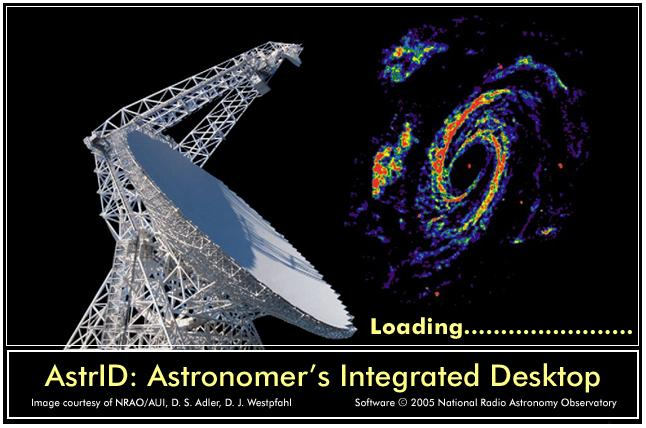
\includegraphics[width=\linewidth]{AstridSplash.jpg}
\captionof{figure}[Astrid splash screen]
{The \gls{Astrid} splash screen.
\label{fig:astridsplash}}
\end{minipage}
\hfill
\begin{minipage}[b]{0.43\linewidth}
\vspace{0pt}
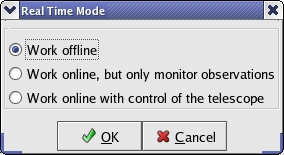
\includegraphics[width=\linewidth]{AstridMode.jpg}
\captionof{figure}[Astrid startup pop-up window]
{\gls{Astrid} startup pop-up window.
\label{fig:astridmode}}
\end{minipage}

\vspace{-5mm}

\subsection{Astrid Modes}\label{sec:astridmode}

\noindent On startup, \gls{Astrid} will automatically ask what mode to operate in via
the pop-up window shown in Figure~\ref{fig:astridmode}.  Once an initial mode has been
set it may be changed at any time by selecting {\tt Real Time Mode...} from the {\tt File}
drop-down menu (see \S~\ref{sec:dropdownmenus}).

{\bf Note} that observers should use {\tt File}$\rightarrow${\tt Real Time Mode...} to
relinquish control of the telescope immediately after their scheduled observing session.

\begin{table}[!h]
\begin{center}
\caption[Astrid online and offline modes]{\gls{Astrid} mode features}\label{table:astridmodes}
\begin{tabular}{lccccl}
\toprule
{\bf Mode}             & Edit \&         &  Validate      & Submit     & Observing & \multicolumn{1}{c}{Data}    \\
                       & Validate Syntax &  Configuration & \glspl{SB} &   Logs    & \multicolumn{1}{c}{Display} \\
\midrule
{\bf Offline}          & \checkmark      & Simulated      &            &           & Historical$^{(1)}$ \\
{\bf Online (monitor)} & \checkmark      & Simulated      &            &\checkmark & Real-time \\
{\bf Online (control)} & \checkmark      & Real$^{(2)}$    & \checkmark$^{(3)}$ &\checkmark & Real-time \\
\bottomrule
\end{tabular}
\footnotesize{
\begin{itemize}[itemsep=0pt]
\item[$(1)$] Previously acquired data should always be viewed \sq{offline}.
\item[$(2)$] Requested configurations are validated with respect to the actual
{\tt dev\_health.conf} file rather than\newline the simulated \sq{ideal} universal cabling file.
\item[$(3)$] Only permitted when you are \sq{in the gateway} (the \gls{GBT} operator has given you
security access).
\end{itemize}
}
\end{center}
\end{table}

\noindent The features available for each mode are listed in
table~\ref{table:astridmodes}.  Users should select the most appropriate
mode for their purposes:

\begin{itemize}[leftmargin=*]
\item {\bf Work offline}: Primarily used to create, edit and validate \glspl{SB}.
It is also the preferred method to look at previously obtained data in the Data
Display since online modes will continually refresh the display window with
near-real-time data.

\item {\bf Work online, but only monitor observations}: May be used to view what
is happening in the \gls{Astrid} observing logs and Data Display for the current
observations. You will not be able to submit \glspl{SB} or affect observing in any
manner.

\item {\bf Work online with control of the telescope}: Used to perform observations
with the \gls{GBT} by allowing the user to submit \glspl{SB}. Log information and
real-time data displays are also available in this mode.
{\bf Note that working online requires the \gls{GBT} operator to \dq{put you
in the gateway} (give you security access).}
\end{itemize}

\newpage

\section{Astrid GUI Composition}\label{sec:astridcomposition}

The \gls{Astrid} \gls{GUI} layout consists of several components shown in
Figure~\ref{fig:astridcomposition} and described in the following section.

\begin{figure}[!h]
\begin{center}
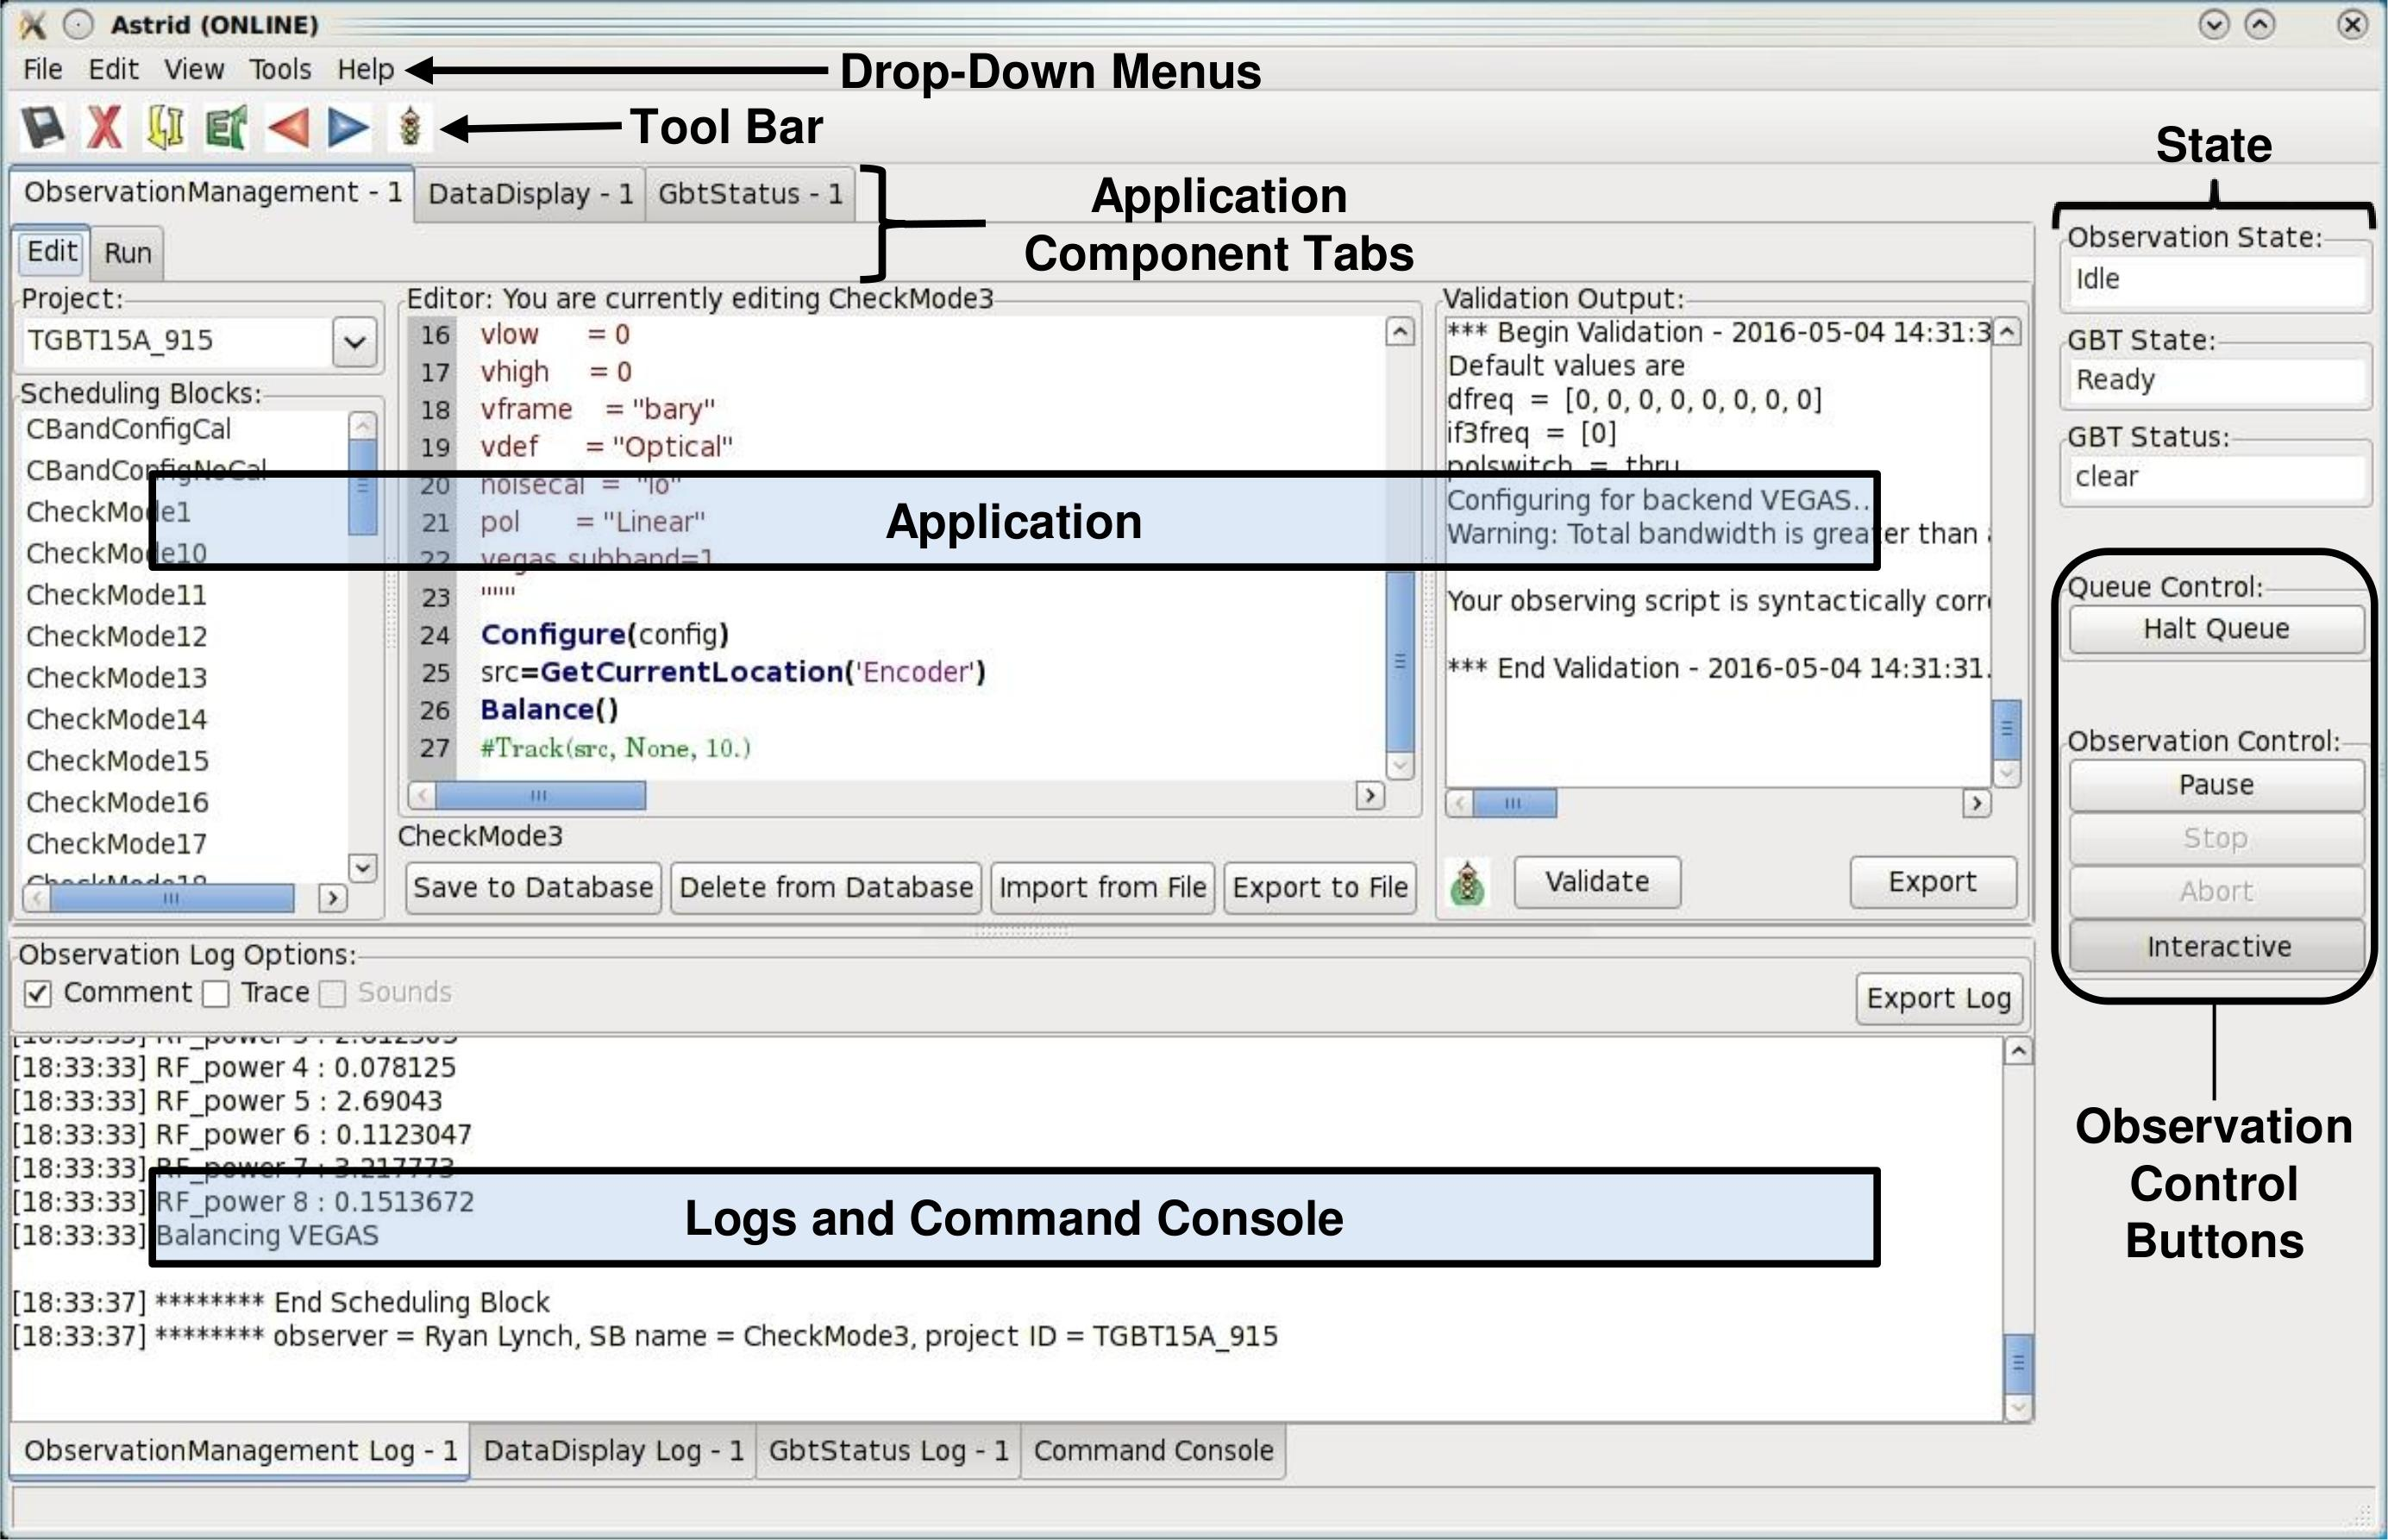
\includegraphics[width=\linewidth]{Astrid_components.jpg}
\caption[Components of the Astrid GUI]
{The different components on the \gls{Astrid} \gls{GUI}.
\label{fig:astridcomposition} }
\end{center}
\end{figure}

\subsection{Resizing Astrid Display Areas}

It is possible to resize some of the display areas within \gls{Astrid}.  If 
you put the mouse over the bar separating two display areas you will
get a double-arrowed resize cursor.  If you then hold down the
left--mouse button you can use the mouse to move the border and resize
the display areas.

\subsection{Application}

This comprises the majority of the space within the \gls{Astrid} \gls{GUI}.  This 
shows the contents of the Application selected by the application component tabs.

\subsection{Application Component Tabs}

The application component tabs are located under the Drop-down menus and the Toolbar
The top level of tabs allow users to switch between the three main \gls{Astrid}
applications: Observation Management, Data Display, and GBT Status.  Below these
are a set of subtabs that vary for each application component tab.

\newpage

\subsection{Drop--down Menus}\label{sec:dropdownmenus}

In the top, left hand side of the \gls{Astrid} \gls{GUI} you will find the drop--down
menus.  The contents of the drop--down menus change according to which
Application is currently being displayed on the \gls{Astrid} \gls{GUI}.  We will
not discuss all of the options under the drop-down menus in this document
but we will provide some highlights.

\begin{description}[leftmargin=*]
\item[File]
\begin{itemize}[itemsep=0pt,leftmargin=*]
\item[-] {\bf New Window} Launch applications within the \gls{Astrid} \gls{GUI} or in an
independent \gls{GUI}.
\item[-] {\bf Close Window} Close the currently displayed application in the \gls{Astrid}
\gls{GUI}.
\item[-] {\bf Real Time Mode...} Change between the operational modes of \gls{Astrid} (see
\S~\ref{sec:astridmode}).
\end{itemize}

\item[Edit] Standard \dq{Windows} undo, redo, cut and paste options.

\item[View] Display or hide the Toolbar or view \gls{Astrid} in Full Screen mode.

\item[Tools] Only active for the Data Display Application.  You may use checkboxes to
select various tooltips such as {\tt info}, {\tt pan}, and {\tt zoom}.  You can also
change the \dq{Fitting Heuristics} used during the reduction of Pointing and Focus
Observations by selecting {\tt Options...} (see \S~\ref{sec:heuristics}).

\item[Help] Bring up documentation for some but not all Applications.

\end{description}


\subsection{Toolbar}

The Toolbar is located just under the Drop--down Menus near the top of the
\gls{Astrid} \gls{GUI}.  The contents of the Toolbar change depending on which
Application is being displayed in the \gls{Astrid} \gls{GUI}.  The Toolbar options
are a subset of commonly used options from the Drop--down Menus.  When you leave
the mouse situated over one of the Toolbar buttons for a few seconds a \dq{pop-up}
will appear that tells you what action the Toolbar button will invoke.

\subsection{Logs}
The Log Window is located in the lower portion of the \gls{Astrid} \gls{GUI}
underneath the Application display area.  Clicking on the log tabs at the very bottom
of the \gls{GUI} will display log information for the Observation Managament, Data Display,
or GBT Status applications.  Viewing a specific log will also change the application
window to display the matching application.

The contents of the Observation Management application Log may be saved to an external
file via the \astridbutton{Export Log} button.  Note that closing or restarting \gls{Astrid} will
clear the Observation Management Log.  If you wish to retrieve an unsaved observating log,
please contact your \gls{GBT} \dq{Friend}.

\subsection{Command Console}
The Command Console is a Python shell that imports the \dq{Configuration Tool} and
\dq{Balance} \glspl{API}.  Both \glspl{API} will only interact with the \gls{MC}
systems if the user has been granted security access and is operating \gls{Astrid}
from the \dq{Work online with control of the telescope} mode (see \S~\ref{sec:astridmode}).

Observers may find the Command Console useful as a stand alone Python Shell.  However,
the \dq{configuration tool} and \dq{Balance} \glspl{API} are only intended for use by
\gls{GBT} staff and expert users.  Note that internal \gls{Astrid} commands
such as those listed in Chapter~\ref{chap:scripts} are not available for use without
first importing all necessary \gls{Astrid} modules.

\newpage

\subsection{State}\label{sec:GBTstatusDescription}

Three indications of state are located in the upper right corner of the \gls{Astrid}
\gls{GUI}.

\begin{description}[leftmargin=*,itemsep=0pt]
\item[Observation State] indicates \textbf{\gls{Astrid}'s state}.\\
If \gls{Astrid} is not communicating with the \gls{MC} system (such as in its
\dq{offline} mode) then you will see \dq{Not Connected}.  If \gls{Astrid} is
communicating with the \gls{MC} system and there isn't an \gls{SB} being executed
then you will see \dq{Idle} and if an \gls{SB} is running (or has been paused)
then you will see \dq{SB Executing}(\dq{SB Paused}). 

\item[GBT State] indicates the \textbf{\gls{MC} system state}.\\
If the \gls{MC} system is not working properly you will see \dq{Not In Service}
or \dq{Not Connected.} \dq{Unknown} indicates that the \gls{MC} system is working
but does not know the state of any of the hardware devices.  You will see the state
be \dq{Ready} when the \gls{GBT} is not doing anything.  It will be \dq{Activating}
or \dq{Committed} when the \gls{GBT} is preparing to perform an observation, etc.
While taking data during a scan the state will be \dq{Running}.  At the end
of a scan you will see the state become \dq{Stopping.}  If the scan is ended
for any abnormal reason the state will be \dq{Aborting.}

\item[GBT Status] indicates the \textbf{error state of the \gls{MC} system}.\\
If the \gls{MC} system is not communicating properly with the hardware the status can
be \dq{Unknown} or \dq{Not Connected.}  If the status is \dq{Clear}, \dq{Info},
or \dq{Notice}  then there are no significant problems with the \gls{GBT}.
If \dq{Warning} then it is worth asking the Operator what the problem is, but
it may not affect observation quality.  If the status is \dq{Error} then there
is potentially something wrong that may need attention. If the status is
\dq{Fault} or \dq{Fatal} then something has definitely gone wrong with the
observations.
\end{description}


\subsection{Observation Control Buttons}

The Observation Control Buttons are located in the lower-right of the \gls{Astrid}
\gls{GUI}. These buttons give the observer control of the \gls{GBT} during the
execution of an \gls{SB} and have the following functions:

\begin{itemize}[leftmargin=\widthof{\astridfixedbutton{Halt Queue}{6em}}]
\item[\astridfixedbutton{Halt Queue}{6em}] If this button is not activated then the \glspl{SB} in the Run queue
will continue to be executed in order. If this button is activated it will finish the current
\gls{SB} but will not allow the next \gls{SB} in the Run Queue to execute until the button
is returned to its default \dq{off} state.
\item[\astridfixedbutton{Pause}{6em}] Stop the execution of the current \gls{SB} when the next line of
code is encountered.
\item[\astridfixedbutton{Stop}{6em}] Stop the current scan at the end of the next integration time.
This is a nice, gentle way to stop a scan.
\item[\astridfixedbutton{Abort}{6em}] Stop the current scan immediately.  This may lead to corrupted data.
\item[\astridfixedbutton{Interactive}{6em}] When selected, will cause \gls{Astrid} to automatically
answer any pop--up query.  \gls{Astrid} will always choose what it deems
to be the safest answer.  This is useful when you have to leave the 
control for an extended period of time (such as when you go to the
cafeteria to eat, etc.).
\end{itemize}

\newpage

%++++++++++++++++++++++++++++++++++++++++++++++++++++++++++++++++++++++++++++
\section{The Observation Management Tab}

The Observation Management Application consists of two sub--\glspl{GUI},  the
Edit Subtab and the Run Subtab (see Figures~\ref{fig:astridedit} 
and~\ref{fig:astridrun}).  In the Edit Subtab you can create, load, save,
and edit \glspl{SB}.  You can also Validate that the syntax is correct.
The Run Subtab is where you will execute \gls{GBT} observations.
 
\subsection{The Edit Subtab}\label{sec:editsubtab}

The Edit Subtab has five major areas: a list of Project Names, \glspl{SB}
that have been saved into the \gls{Astrid} database for that project, an
editor, a Validation area, and a log summarizing the observations. This is
shown in Figure~\ref{fig:astridedit}. Chapter~\ref{chap:scripts} covers the
contents and creation of \glspl{SB}.

\begin{figure}[!h]
\setlength{\abovecaptionskip}{0pt}
\begin{center}
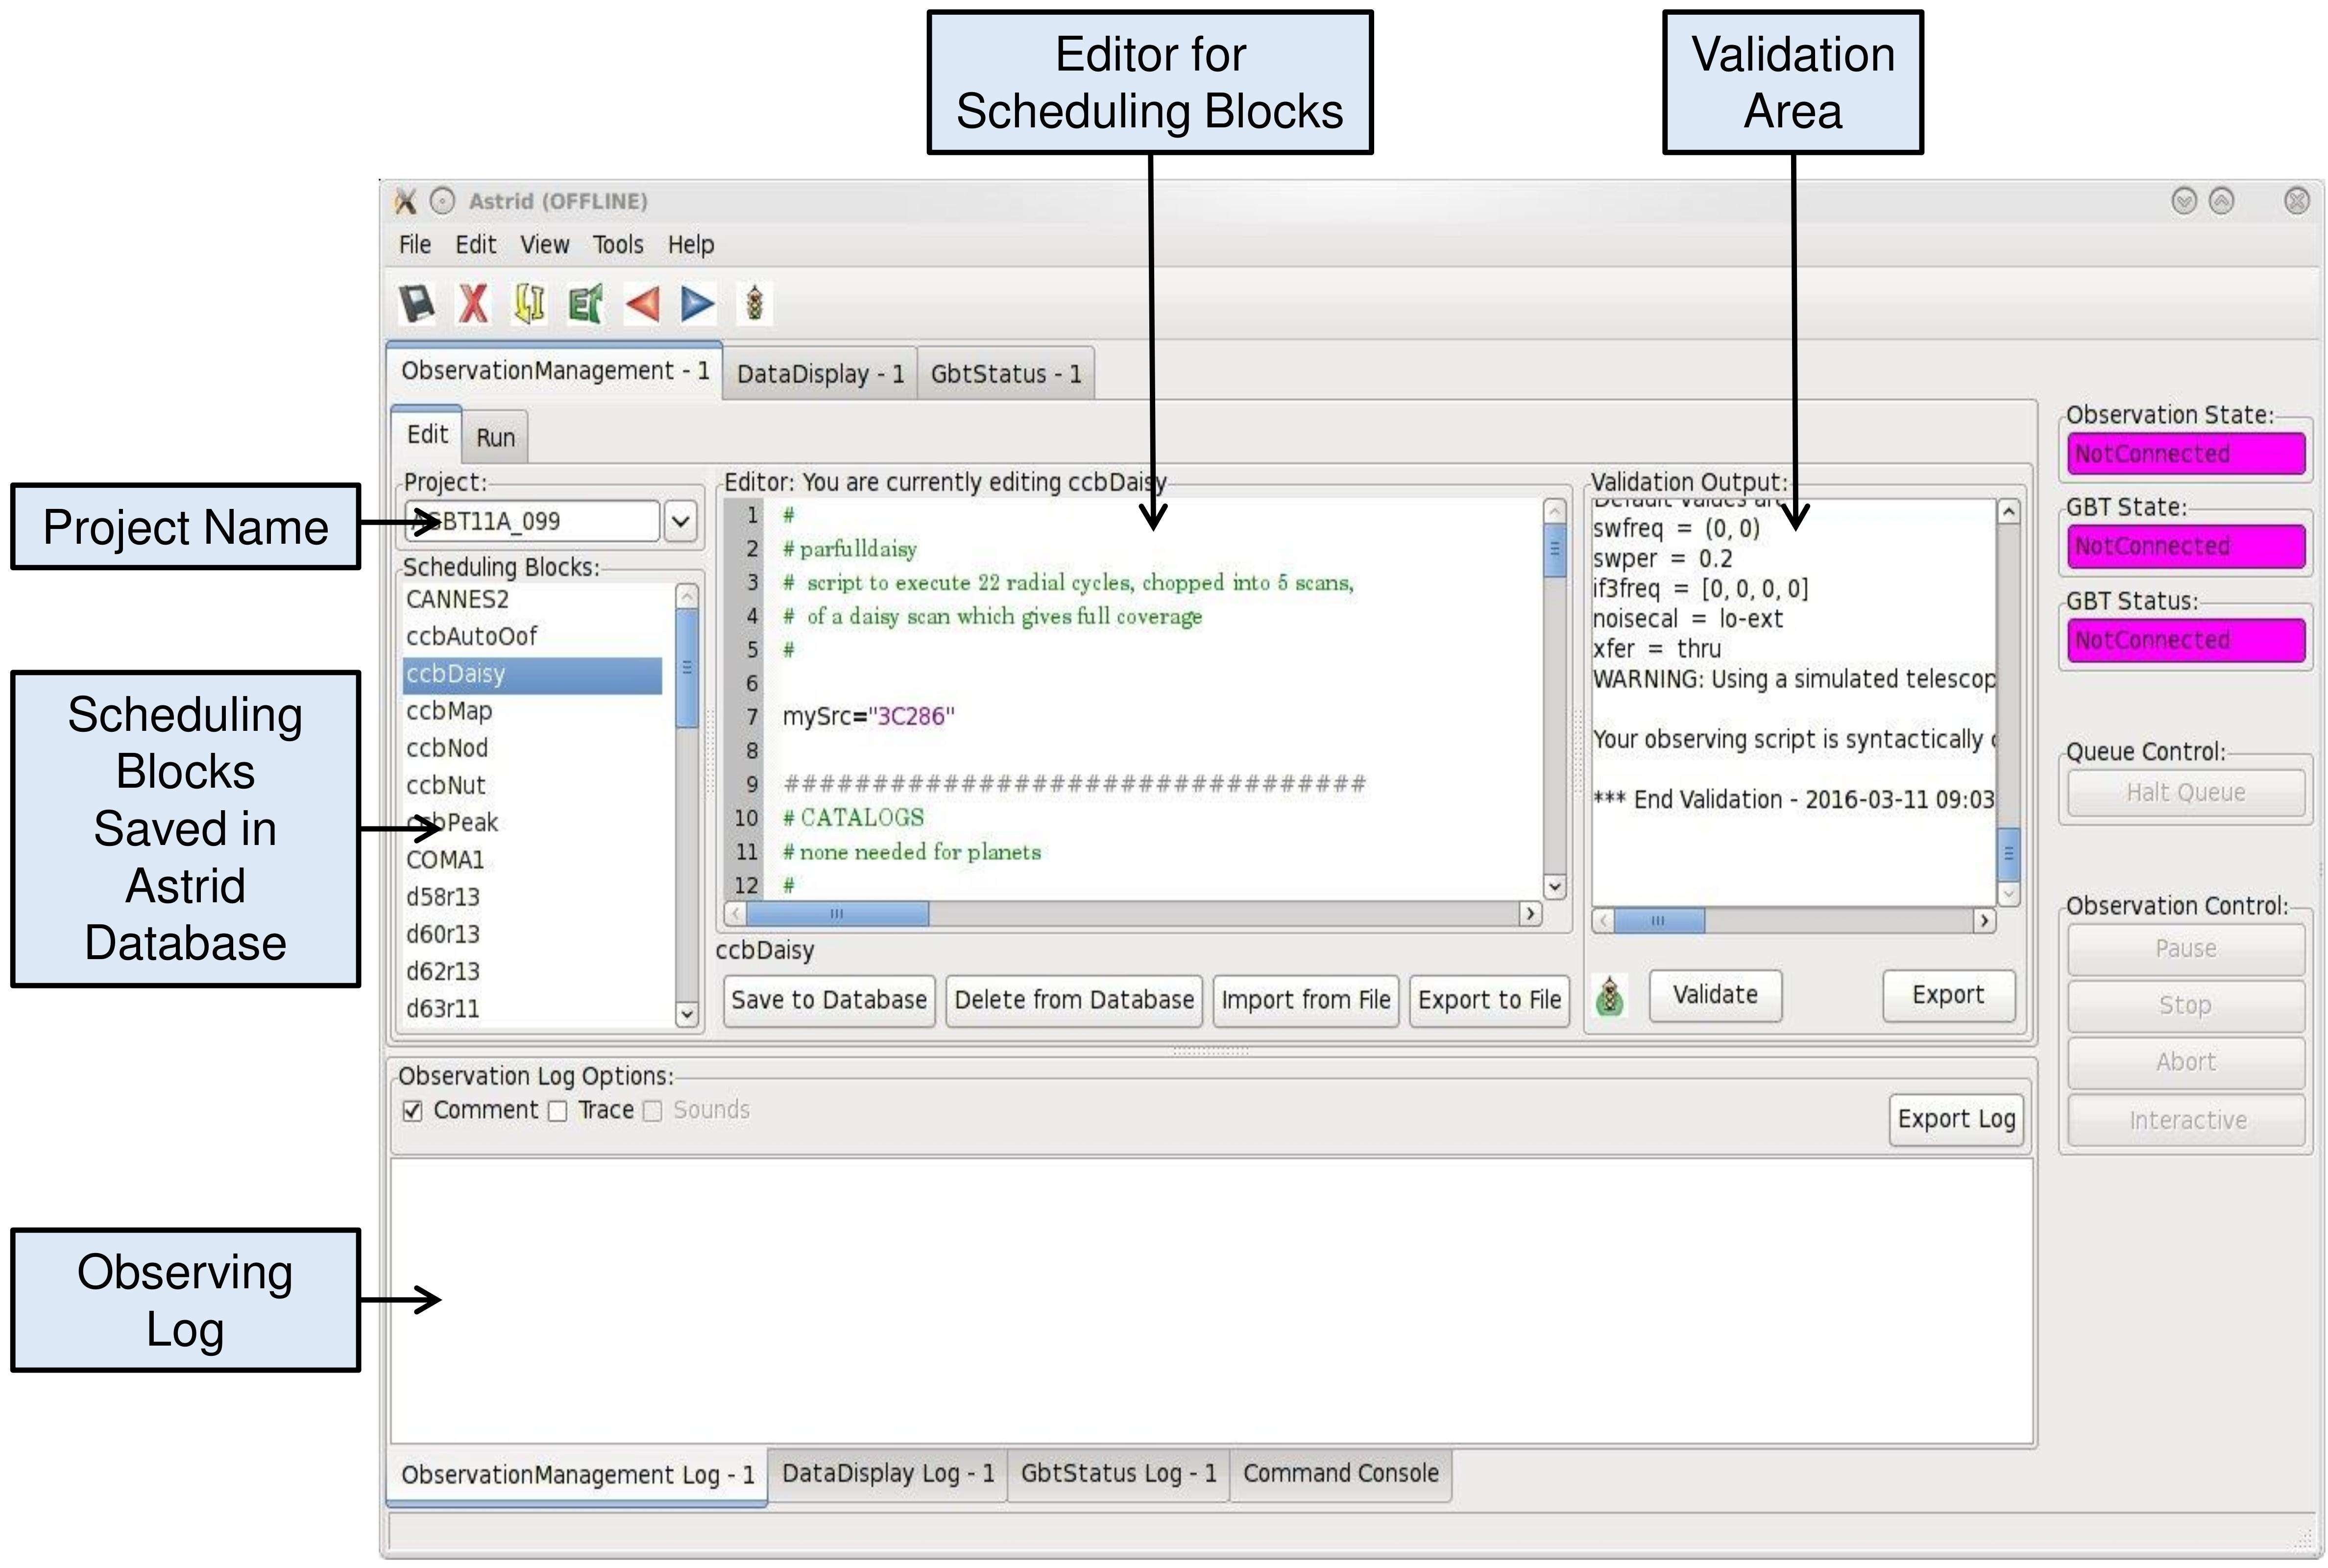
\includegraphics[width=0.90\linewidth]{AstridEditSubtab.jpg}
\caption[Astrid Observation Management/Edit Subtab]
{The \gls{Astrid} Observation Management/Edit Subtab. \label{fig:astridedit} }
\end{center}
\end{figure}

\subsubsection{Project Name and List of Scheduling Blocks}
\label{sec:projectID}
To access scheduling blocks associated with your project, you will need to
enter your Project Name in the \dq{project} window located in the upper left
part if the Edit Subtab.  Your Project Name is the code that your \gls{GBT}
proposal was given with the prefix \dq{AGBT}, e.g., AGBT16A\_001. To enter a
Project Name you may either type it in directly, or use the drop--down
arrows to navigate to your project through a project hierarchy as shown in
Figure~\ref{fig:projectHierarchy}

After doing this you will see in the window labeled \dq{Scheduling Blocks}
a list of \glspl{SB}, if any, that have been previously saved into the
\gls{Astrid} database. All of the saved \glspl{SB} for a given project will
show up in the \dq{Scheduling Blocks} section of the Edit Subtab.  If an \gls{SB}
has been Validated (i.e. it is syntactically correct) then it will appear
in bold--face type.  This means that it can be executed.  If the script
has been saved but is syntactically incorrect it will appear in  
lighter--faced type.

\newpage

\begin{figure}[!h]
\setlength{\abovecaptionskip}{0pt}\setlength{\belowcaptionskip}{0pt}
\begin{center}
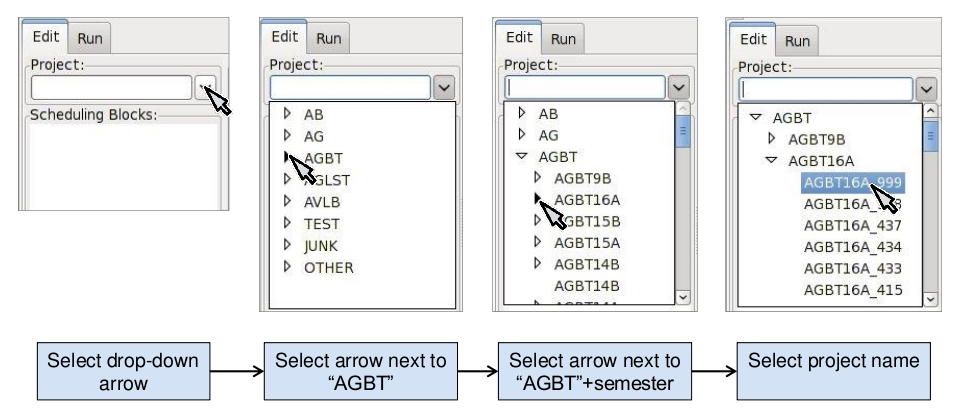
\includegraphics[width=0.9\linewidth]{projectHierarchy.jpg}
\caption[Selecting your project using the drop-down menu]
{Selecting your project using the drop-down menu. \label{fig:projectHierarchy} }
\end{center}
\end{figure}

\subsubsection{Editor}\label{sec:astridimport}

You can use the Editor to create or modify an \gls{SB} within \gls{Astrid}.  Standard
Windows functions like Ctrl--X (to cut selected text), Ctrl--C (to
copy selected text), and Crtl--V (to paste selected text) can be used within
the editor.  The editor lists the line number on the left hand side of the
window and marks Python code as follows:

\begin{itemize}[itemsep=0pt]
\item \textbf{\textcolor{pythonComments}{Green highlighted text}} - Commented characters
\item \textbf{Black highlighted text} - Standard Python commands/syntax
\item \textbf{\textcolor{pythonStrings}{Purple highlighted text}} - Strings
\item \textbf{\textcolor{pythonTripleStrings}{Magenta highlighted text}} - Triple quoted strings
(used in Python to enclose strings that span multiple lines)
\item \textbf{\textcolor{pythonKeywords}{Dark blue highlighted text}} - Python functions
\item \boldmath{$\ominus$}/\boldmath{$\oplus$} - Marks the start of an indented block of Python code
such as an {\bfseries{\textcolor{pythonKeywords}{if}}} statement or
{\bfseries{\textcolor{pythonKeywords}{for}}} loop.  Clicking on $\ominus$ will
collapse the indented code block and change the symbol to $\oplus$.  Likewise,
clicking on $\oplus$ will expand a previously collapsed code block.
\end{itemize}

\noindent The editor also has four operational buttons:

\begin{itemize}[itemsep=0pt,leftmargin=\widthof{\astridfixedbutton{blah}{10em} -}]

\item[\astridfixedbutton{Save to Database}{10em} -] This button will check the validation of the
current \gls{SB} and then save it to the \gls{Astrid} database.  A pop--up
window will notify you if the \gls{SB} did not pass Validation.  A second
pop-up window will allow you to set the name that the \gls{SB} will be saved
under in the \gls{Astrid} database.
\item[\astridfixedbutton{Delete from Database}{10em} -] This button will delete the currently selected
\gls{SB} from the \gls{Astrid} database.
\item[\astridfixedbutton{Import from File}{10em} -] This button will allow you to load an \gls{SB} from
a file on disk.
\item[\astridfixedbutton{Export to File}{10em} -] This button will allow you to save the edited \gls{SB}
displayed in the editor to a file on a disk.  This does not save the \gls{SB}
into the \gls{Astrid} database.
\end{itemize}

The first time you select either of the \astridbutton{Import from File} or
\astridbutton{Export to File} buttons you will have a pop--up window that
lets you select the default directory to use.  After selecting the default
directory you will get a second pop--up window that shows the contents of the
default directory so that you can select or set the disk file name to load
from or export to.

\newpage

\subsubsection{Adding and Editing Scheduling Blocks in the Database}

We will first describe how to add an \gls{SB} to the \dq{Scheduling Block} list
(i.e. database) and then we will describe how to manipulate and edit \glspl{SB}
in the list.

\begin{description}[leftmargin=*]

\item[Saving a Scheduling Block to the Database]\ \\
If you have already created an \gls{SB} outside of \gls{Astrid}, you should go to the
Edit Subtab in \gls{Astrid} and then use \astridbutton{Import from File} to load
your \gls{SB} into the Editor.  Otherwise you can just create your \gls{SB} in the
Editor.  To save the \gls{SB} into the \gls{Astrid} database you just need to hit
\astridbutton{Save to Database}.  This will run a validation check
(see \S~\ref{sec:validation}) on your \gls{SB} and then a pop--up window will appear
which allows you to specify the name which you would like to use in the list for your
\gls{SB}.

\item[Selecting a Scheduling Block]\ \\
If you perform a single click on any \gls{SB} in the \dq{Scheduling Block} list,
the contents of the selected \gls{SB} will appear in the Editor.  The selected \gls{SB}
will be highlighted with a blue background.

\item[Mouse--button Actions on the selected Scheduling Block]\ \\
If you perform a right mouse button click on the selected \gls{SB} a pop--up window
will appear that will let you rename, create a copy or save the \gls{SB} to the
\gls{Astrid} database.  You can also delete the \gls{SB} from the \gls{Astrid} database.
You may also rename the \gls{SB} if you perform a left mouse button double click
on the script name in the list.

\end{description}


\subsubsection{Validator}\label{sec:validation}

The Validation area is where you can check that the currently selected 
\gls{SB} is syntactically correct.  This does not check for run--time errors
and thus, does not guarantee that the script will do exactly what you want it to do.
For example, it can not check that you have the correct coordinates for your source.
You will also see error messages, notices and warnings from the Validation in this area.

The Validator will attempt to verify that you are using a legal configuration.
When run in \gls{Astrid}'s offline mode, the Validator can only compare your requested
configuration with a simulated \dq{ideal} model of the telescope hardware. To perform a
full configuration check against the true hardware state of the telescope (modelled by the
{\tt dev\_health.conf} file), you must be running \gls{Astrid} from the \dq{Work online
with control of the telescope} mode.

Before an \gls{SB} can be run within \gls{Astrid} it first must pass Validation.  To
Validate a script without saving it you can just hit \astridbutton{Validate}.
An \gls{SB} automatically undergoes a validation check when you hit
\astridbutton{Save to Database} in the editor.  Any messages, etc. from the
validation will appear in the \dq{Validation Output} test area. You can export
these messages to a file on disk by hitting \astridbutton{Export} in the
validation area.

The state of an \gls{SB}'s validation is shown by the stop--light. If the script has
never been validated or has been changed since the last validation the
stop--light will have the yellow light on.  If the \gls{SB} fails validation the
stop--light will turn red, while it will turn green if the \gls{SB} passes validation.

\noindent {\bf Note:} {\bfseries{\textcolor{pythonKeywords}{for}}} loops with many
repeats can take an extended amount of time to validate since the Validator will
go through each step in the loop. Also be careful of infinite loops in the
validation process.  Use of time functions such as
{\bfseries{\textcolor{pythonKeywords}{Now}}()} (see Chapter~\ref{chap:scripts})
always return \dq{None} in the validation.

\subsubsection{The Observing Log}

The observing log is always visible at the bottom of the Observation Management
Tab.  It shows information from the execution of \glspl{SB} in either of the
\gls{Astrid} online modes.  The observing log can be saved to a disk file
by hitting the \astridbutton{Export} button that is just above the top right corner of the
log display area.  Note that closing \gls{Astrid} will clear the observing log.
If you wish to retrieve unsaved observing log information, please contact your
\gls{GBT} \dq{friend}.


\newpage


\subsection{The Run Subtab}\label{sec:runsubtab}

The Run Subtab is shown in Figure~\ref{fig:astridrun}.  Here you will queue up
\glspl{SB} to perform the various observations that you desire to make. The Run
Subtab has five components.  Across the top of the Run Subtab you enter
information that will be put into the headers associated with the observations.
On the left is a list of \glspl{SB} that you can execute.  On the right are the
\dq{Run Queue} which holds \glspl{SB} that are to be executed in the future,
and the \dq{Session History} which shows which \glspl{SB} have previously been
executed.  At the bottom is the \dq{Observing Log}.

\begin{figure}[!h]
\begin{center}
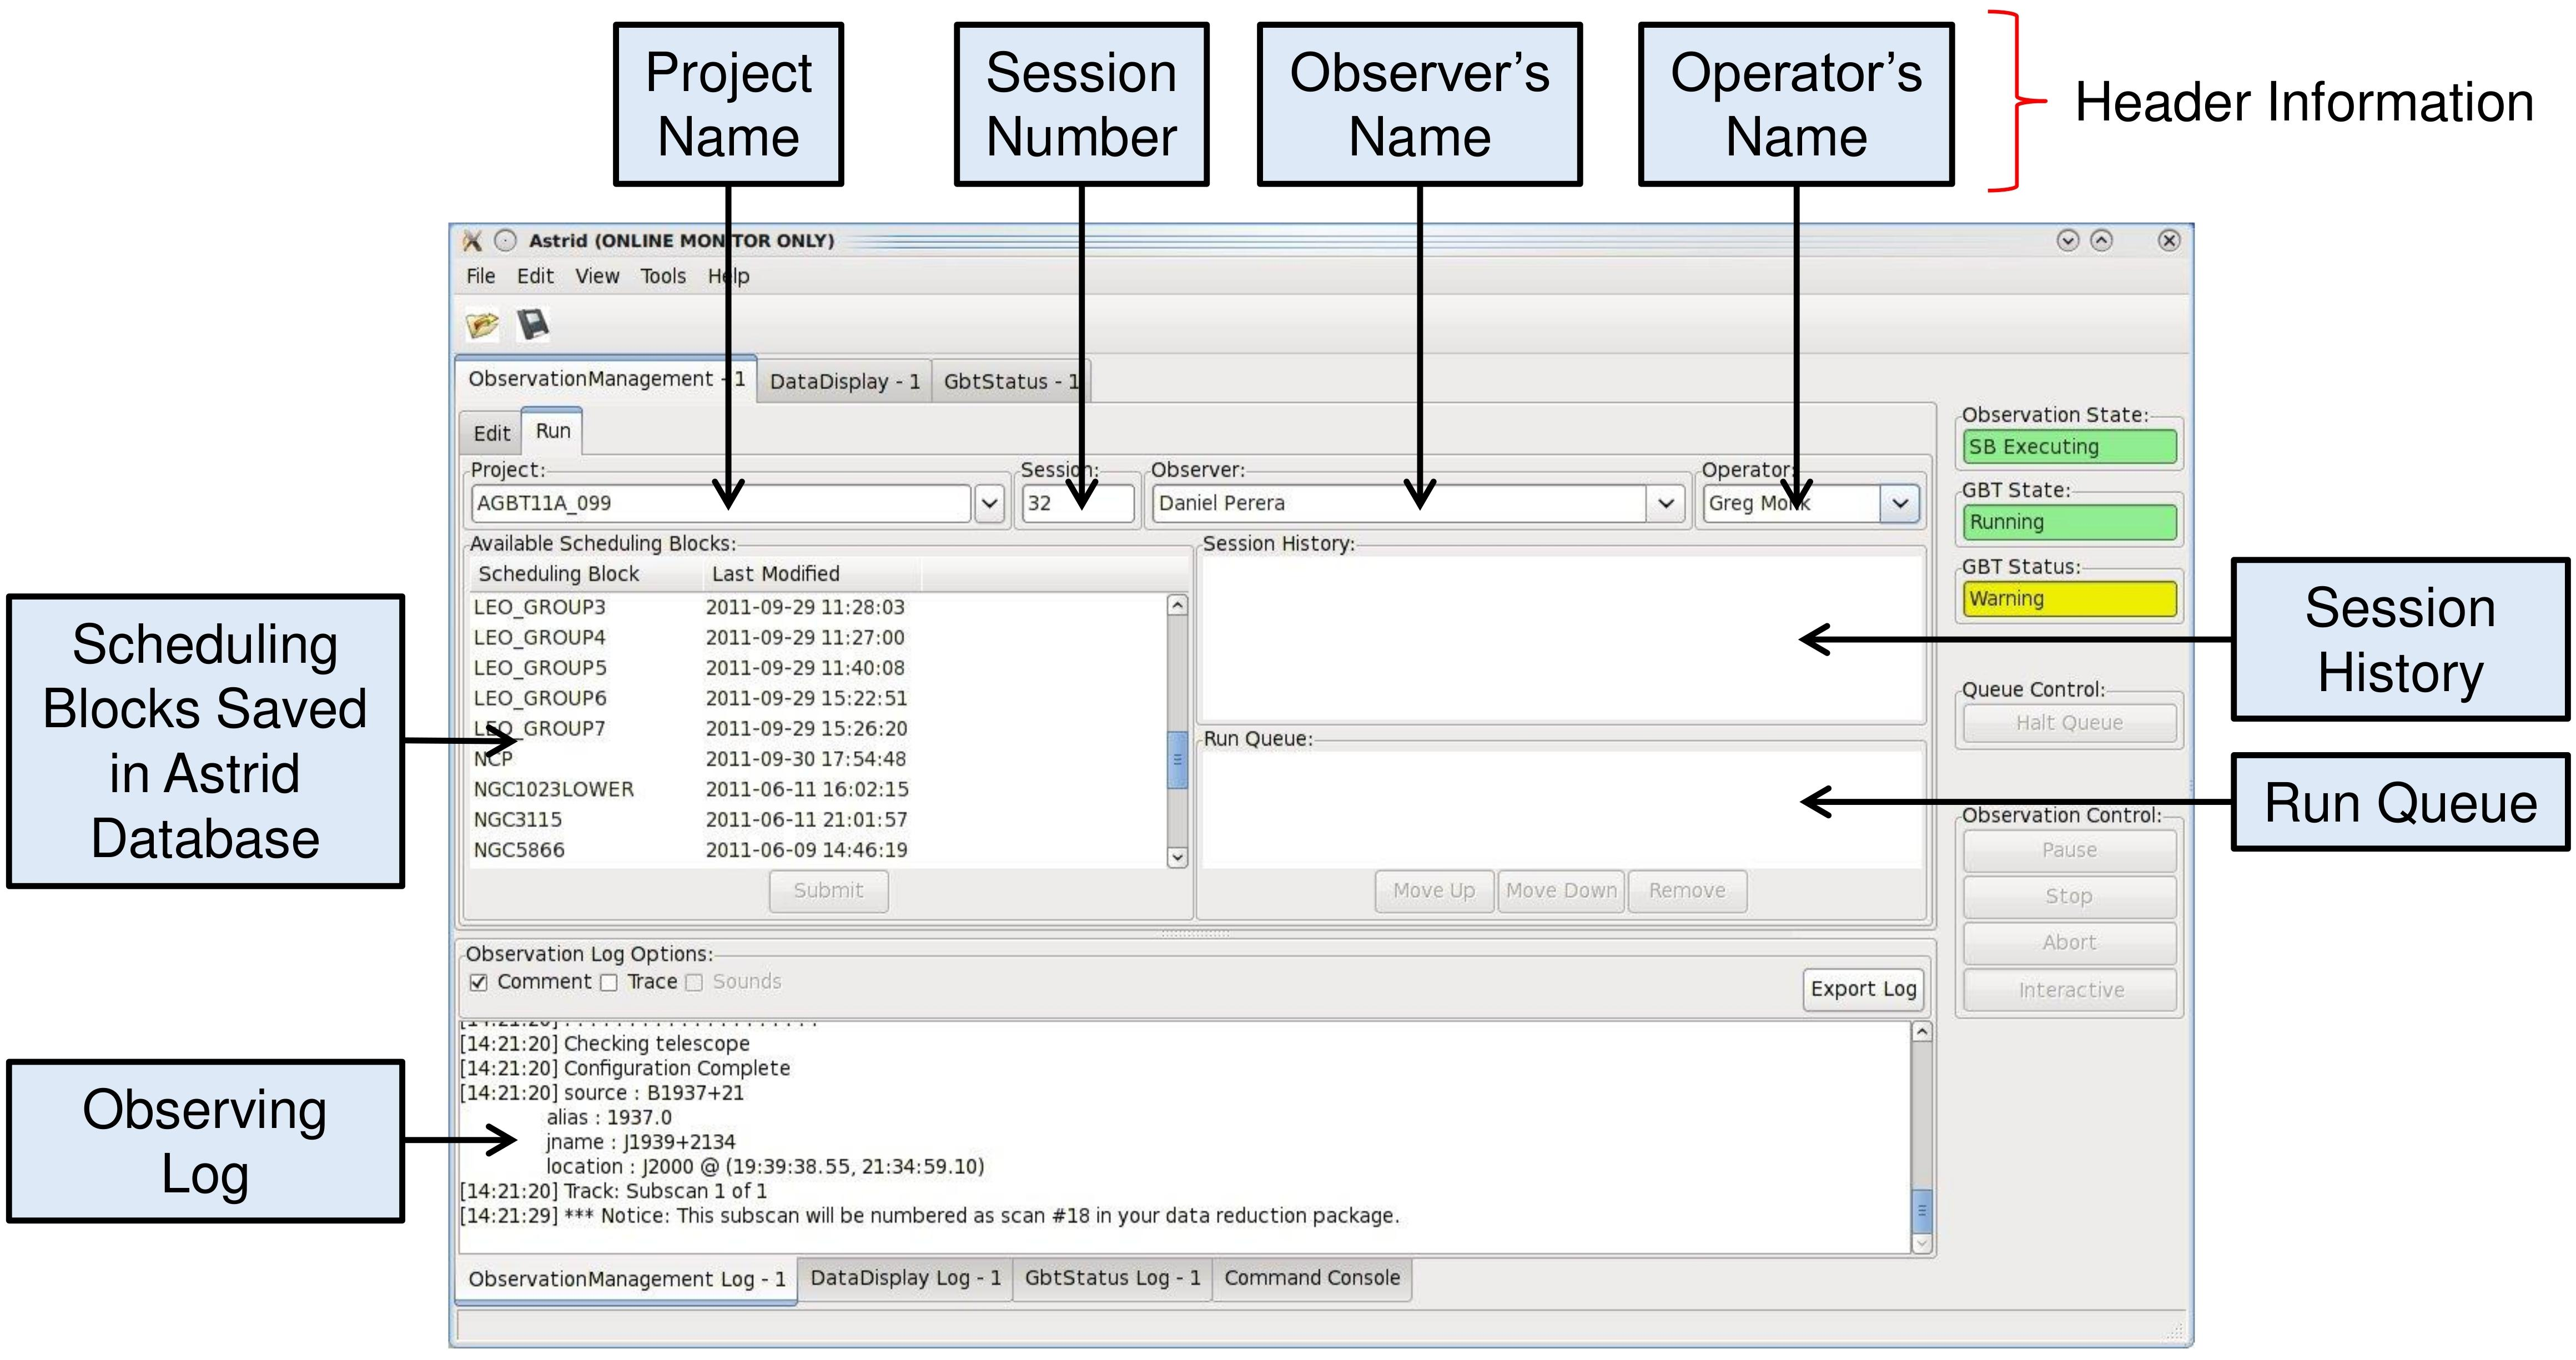
\includegraphics[width=\linewidth]{AstridRunSubtab.jpg}
\caption[Astrid Observation Management/Run Subtab]
{The \gls{Astrid} Observation Management/Run Subtab. \label{fig:astridrun} }
\end{center}
\end{figure}

\subsubsection{Header Information Area}

The following fields must have entries before an \gls{SB} can be executed:
\begin{description}[leftmargin=*]
\item[Project:] Just as in the Edit Subtab you use the drop--down menu to select
your Project Name. If your project is not listed, ask your \gls{GBT} \dq{friend} or the
telescope Operator to add it to the database.
\item[Session:] A session is a contiguous amount of time (a block of time) for which
the project is scheduled to be on the telescope.  Each time a project begins
observing for a new block of time it should have a new session number. The session
number is usually determined by \gls{Astrid} and automatically entered. However, there
are cases (such as \gls{Astrid} crashing) where the session number could become
incorrect.  You can type in the correct session number if needed. {\bf Note that a
\dq{Session} in \gls{Astrid} is equivalent to an \dq{observing period} in the lingo of the
\glsfirst{DSS}. \dq{Session} has a different meaning in the \gls{DSS}.}
\item[Observer's Name:] This is a drop--down list where you choose the observer's
name.  Only the \glspl{PI} on a project are guaranteed to have their name in this list.
If your name is not listed, ask your \gls{GBT} \dq{friend} or the telescope operator to
add it.
\item[Operator's Name:] This is a drop--down list from which you pick the current
operator's name at the beginning of your observations.
\end{description}

\newpage

\subsubsection{Submitting An SB to the Run Queue}

In order to execute an \gls{SB} you must:
\begin{enumerate}[label=\bfseries{Step \arabic*.},leftmargin=*,
labelindent=\parindent, itemsep=1pt]
\item Select the Observation Management Tab. 
\item Select the Run Subtab.  
\item Make sure that the header information fields all have entries.  
\item Select the \gls{SB} you wish to execute from the list of available \glspl{SB}.  
\item Hit the \astridbutton{Submit} button below the list of \glspl{SB}.
\end{enumerate}
Your \gls{SB} is then automatically then sent to the Run Queue.  Note that double-clicking
on an \gls{SB} is the same as selecting the \gls{SB} and then hitting \astridbutton{Submit}.

\subsubsection{The Run Queue and Session History}

When an \gls{SB} is submitted for execution it is first sent to the Run Queue.  This
contains a list of submitted \glspl{SB} that will be sequentially executed in the future.

When an \gls{SB} begins execution it is moved to the Session History list.  So the
Session History list contains the currently executing \gls{SB} on the first line and all
previously executed \glspl{SB} that have been run while the current instance of \gls{Astrid}
has been running on subsequent lines.

If there are not any \gls{SB} in the Run Queue when a new \gls{SB} is submitted
for execution it may appear that the \gls{SB} just shows up in the Session History.
However it has indeed gone through the Run Queue - albeit very quickly.

\subsubsection{The Observing Log}

The observing log is always visible at the bottom of the Observation Management
Tab.  It shows information from the execution of \glspl{SB}.  The observing log can be
saved to a disk file by hitting the \astridbutton{Export} button that is just above the top right
corner of the log display area.  Note that closing \gls{Astrid} will clear the observing log.
If you wish to retrieve unsaved observing log information, please contact your \gls{GBT}
\dq{friend}.

%++++++++++++++++++++++++++++++++++++++++++++++++++++++++++++++++++++++++++++
\section{The Data Display Tab}
 
The Data Display Tab provides a near--real time display of your \gls{GBT} data and
is discussed in Chapter~\ref{chap:datadisplay}.
\newpage
%++++++++++++++++++++++++++++++++++++++++++++++++++++++++++++++++++++++++++++
\section{The GbtStatus Tab}\label{sec:astridstatus}
 
The GbtStatus Tab displays various \gls{GBT} specific parameters, sampled values and 
computed values. Special care was taken to promote its use for remote 
observing.  An Example of how the \gls{GBT} Status Display appears in \gls{Astrid}
is shown in Figure~\ref{fig:astridstatusone} and~\ref{fig:astridstatustwo}.

\begin{figure}[!h] %general to scan/source
\begin{center}
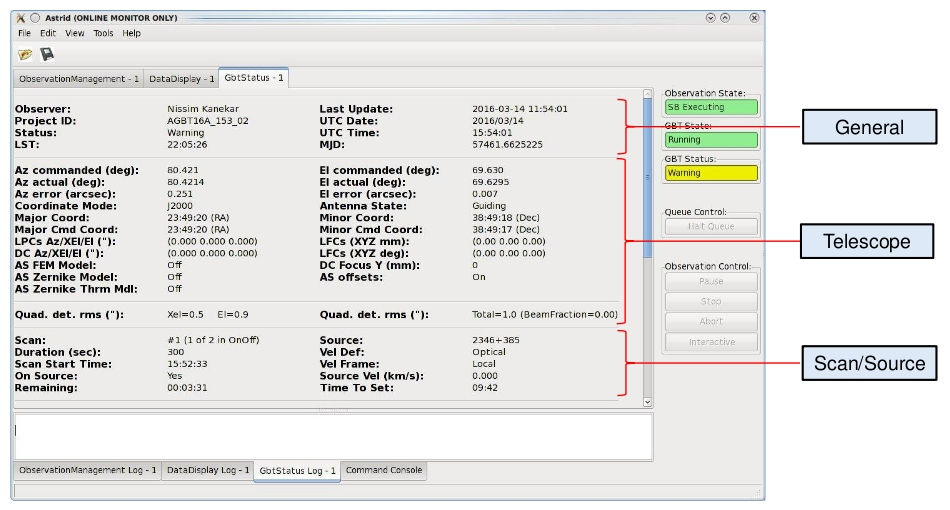
\includegraphics[width=\linewidth]{GBTstatus1.jpg}
\caption[Astrid Status Tab (top)]{The top portion of the \gls{Astrid} GbtStatus Tab.
To see the rest of the status screen you will need to use the scroll bar. 
\label{fig:astridstatusone} }
\end{center}
\end{figure}

The default status screen displays all of the currently supported items of 
the gbtstatus program grouped into various sections.  These are:

\subsection{General Status}
\begin{description}[leftmargin=*,itemsep=0pt]
\item[Observer:] The observer name.
\item[Project ID:] The data directory of the FITS files.  This is your Project Name
with the session as a suffix.  For example, the Project ID for session 02 of AGBT16A\_001
would be AGBT16A\_001\_02 (See \S~\ref{sec:projectID}).
\item[Status:] The status of the \gls{GBT}.  See \S~\ref{sec:GBTstatusDescription}
\item[LST:] The \glsunset{LST}\glsfirst{LST} of the last update.
\item[Last Update:] The local time when the database was last updated.
\item[UTC Date:] The \glsfirst{UTC} date of the last update. 
\item[UTC Time:] The \glsunset{UTC}\gls{UTC} time of the last update.  
\item[MJD:] The \glsunset{MJD}\glsfirst{MJD} of the last update.
\end{description}

\newpage

\subsection{Telescope Status}
\begin{description}
\item[Az commanded:] The commanded azimuth position of the telescope in degrees.
\item[Az actual:] The actual azimuth position of the telescope in degrees.
\item[Az error:] The difference between the commanded and the actual azimuth 
position of the telescope in arc-seconds.  This value does not contain a 
$\cos\left( {\rm el} \right) $ correction.
\item[El commanded:] The commanded el position of the telescope in degrees.
\item[El actual:] The actual elevation position of the telescope in degrees.
\item[El error:] The difference between the commanded and the actual elevation 
position of the telescope in arc-seconds.
\item[Coordinate Mode:] The coordinate mode used to represent a particular
location on the sky. See \S~\ref{sec:location_objects}
\item[Major and Minor Coord:] The telescope position in the current Coordinate Mode.
\item[Major and Minor Cmd Coord:] The telescope position in the current commanded
Coordinate Mode.
\item[Antenna State:] If the antenna software is not running the state will be
\dq{Disconnected.} If the antenna software is running but with its control of the antenna
turned off then the state is \dq{Dormant.}  If the antenna is not moving then the state
will be \dq{Stopped.}  If the antenna is moving and data are being taken then the state is
\dq{Guiding} and if data are not being taken the state is \dq{Tracking.}  If the antenna is
moving to a new commanded position the state is \dq{Slewing.}
\item[LPCs Az/XEl/El:] The \gls{LPC} offsets in arc-seconds.
\item[DC Az/XEl/El:] The \gls{DC} values in arc-seconds.
The \gls{GBT} has temperature sensors attached at various points on the backup
structure and the feed-arm.  These are used in a dynamic model for how the
\gls{GBT} flexes with changing temperatures.  This model is used to correct for
pointing and focus changes that occur from this flexing.
\item[LFCs (XYZ mm):] The \glsunset{LFC}\glsfirstplural{LFC} for the offset focus
position in millimeters.  This value is determined from a Focus observation
(see Chapter~\ref{chap:scripts}).
\item[LFCs (XYZ deg):] The subreflector tilt offset in degrees.
\item[DC Focus Y (mm):] The \gls{DC} Y subreflector offset in millimeters.
\item[AS FEM Model:] The  state of the \gls{FEM} correction for the \glsfirst{AS}.
The \gls{FEM} predicts how the surface changes due to gravitional flexure versus the
elevation angle.
\item[AS Zernike Model:] The  state of the \gls{AS} Zernike model correction model.
The Zernike model is a set of Zernike polynomial coefficients determined from
Out--Of--Focus holography that improve the shape of the \gls{AS} versus the elevation
angle.
\item[AS Zernike Thrm Model:] The  state of the \gls{FEM} correction for the \gls{AS}.
The \gls{FEM} predicts how the surface changes due to thermal flexure.
\item[AS Offsets:] The  state of the \gls{AS} zero offsets. The zero offsets are the
default positions for the \gls{AS}.  This should always be \dq{On} if the \gls{AS} is being
used.
\item[Quad. det. rms:] The quadrant detector is used to detect and correct for
wind-induced pointing errors.  rms values in arc-seconds are reported in elevation
and cross--elevation.  Total rms is also given as a fraction of the beam.
\end{description}

\subsection{Scan and Source Status}
\begin{description}
\item[Scan:] A scan is a command within an \gls{SB} used to collect observational data.
The field here is derived from the scan number and \gls{PROCNAME}, \gls{PROCSIZE}
and \gls{PROCSEQN} keywords from the \gls{GO} FITS file. 
\item[Duration:] The scan length in seconds.
\item[Scan Start Time:] If scan has started it is the \gls{UTC} scan start time - if the
scan has not started, then it is the countdown until the start of scan. 
\item[On Source:] \dq{Yes} or displays a countdown until the antenna is on source.
\item[Remaining:] The time remaining in the scan.
\item[Source:] The source name.
\item[Vel  Def:] The velocity definition specifies which mathematical equation is used to
convert between frequency and velocity.  See Equations~\ref{eq:vradio},~\ref{eq:voptical},
and~\ref{eq:vrel}
\item[Vel Frame:] The velocity frame or inertial reference frame.  See the \dq{vframe}
keyword in \S~\ref{sec:keywords}
\item[Source Vel:] The source velocity (km\,s$^{-1}$).
\item[Time To Set:] The time till the current source sets. 
\end{description}
\ \newline

\begin{figure}[!h]
\begin{center}
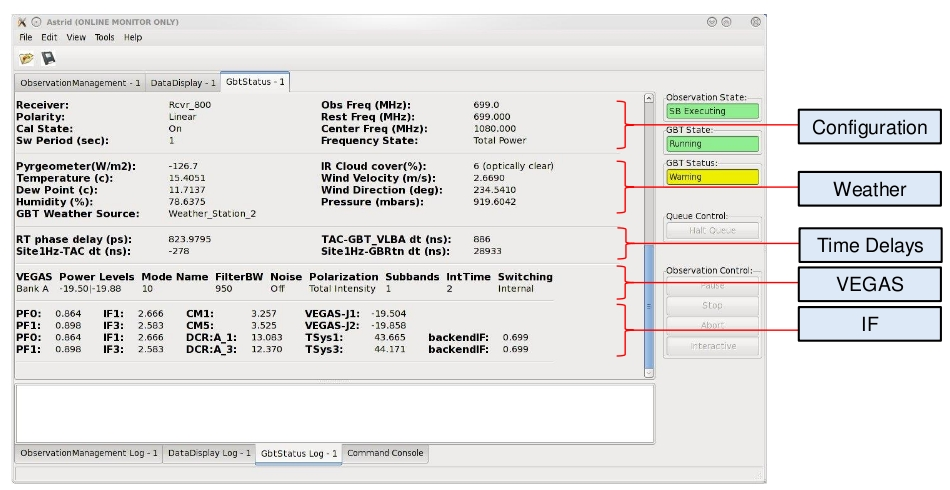
\includegraphics[width=\linewidth]{GBTstatus2.jpg}
\caption[Astrid Status Tab (bottom)]{The top portion of the \gls{Astrid} GbtStatus Tab.
To see the rest of the status screen you will need to use the scroll bar. 
\label{fig:astridstatustwo} }
\end{center}
\end{figure}
\newpage

\subsection{Configuration Status}
\begin{description}
\item[Receiver:] The receiver being used.
\item[Polarity:] The receiver polarity.
\item[Cal State:] \sq{ON} if the \gls{noiseDiode} is firing during the scan. 
\item[Sw Period:] The period in seconds over which the full switching cycle occurs.
This is determined by the user in their configuration (see \S~\ref{sec:config}).
\item[Obs Freq:] The observed spectral line frequency in the local frame (MHz).
\item[Rest Freq:] The spectral line frequency in the rest frame (MHz).
\item[Center Freq:] The center \gls{IF} frequency set by the \gls{LO} in MHz.  See
Appendix~\ref{appendix:spectralwindows} for further details.
\item[Frequency State:] The switching type.  Either \gls{tpower} or \gls{fsw}.
\end{description}

\subsection{Weather Status}

A real--time readout from one of the \gls{GBT} weather stations providing information on
temperature, pressure, humidity, dew point, wind direction and velocity. In addition,
the pyrgeometer measures the net near-IR irradiance of the sky to give an approximate
indication of cloud cover.

\subsection{Time Delay Status}
\begin{description}
\item[RT phase delay:] This is the time delay between the timing center in the \gls{GBT}
equipment room and the \gls{GBT} receiver room, in picoseconds, modulo 2000~ps.  It is measured
by comparing the phase of the 500~MHz reference signal  sent to the receiver room with a
copy of the signal returned to the  timing center.
\item[Site1Hz-TAC dt:] Time difference between the Site1Hz (a one pulse per second signal
that is locked to the hydrogen maser time standard) and a pulse from the GPS receiver
(\dq{TAC})
\item[TAC-GBT\_VLBA dt:] Time difference between the GPS receiver and the \gls{VLBA} back end
timing module.
\item[Site1Hz-GBTRtn dt:] Time delay between the Site 1Hz and a copy of the 1 Hz returned
from \gls{GBT} receiver room.  It is twice the delay of the fiber cables. The value is about
28933~ns which means the time delay between the equipment room the the receiver room is
about 14466~ns.
\end{description}

\subsection{VEGAS Status}
\begin{description}
\item[VEGAS:] The \gls{VEGAS} Bank (spectrometer with letter designation $A \rightarrow H$)
selected in the scan coordinator.
\item[Power Levels:] The power levels at the inputs to the \gls{VEGAS} \gls{ADC} cards.
There are two \glspl{ADC} per bank, one for each polarization. The \gls{VEGAS} balance
\gls{API} sets these values to approximately -20dBm by default.
\item[Mode Name:] Each \gls{VEGAS} Bank can be configured in one of 29 modes (see
Table~\ref{tab:vegas_modes}).
\item[FilterBW:] The bandwidth (MHz) of the digital filter implemented in the
\glsunset{FPGA}\glsfirst{FPGA}.  Note that these values do not correspond to the
bandwidths listed in Table~\ref{tab:vegas_modes}.
\item[Noise:] The state of the noise source which can be either \dq{On} or \dq{Off}.
\item[Polarization:] Users may specify which spectral product to record (See the \dq{vegas.vpol}
keyword in \S~\ref{sec:keywords}).  vegas.vpol=\dq{self} records \dq{Total Intensity} products,
\dq{cross} records \dq{Full Stokes} parameters, \dq{self1} records the polarization inputs
from the first \gls{ADC} only, and \dq{self2} records the polarization inputs from the second
\gls{ADC} only.
\item[Subbands:] Each \gls{VEGAS} bank can select between single (subbands=1) and multiple
(subbands=8) spectral windows when using VEGAS modes with a 23.44~MHz bandwidth.  
\item[IntTime:] The \gls{VEGAS} integration (dump) time in seconds.
\item[Switching:] Determines whether switching is controlled by \gls{VEGAS} (\dq{Internal}) or
another source (\dq{External}).

\end{description}

\subsection{IF Status}

The \gls{IFpath} in use are always displayed in the last section of the \gls{GBT}
status screen.  An example screen is shown in Figure~\ref{fig:astridstatustwo}.
Each line represents the \gls{IFpath} for a single polarization path from the 
\gls{IFRack} to the backend.  Each line contains only the devices in use for the 
listed path. A path may include a subset of the devices and values listed 
below.

\begin{description}[leftmargin=*]
\item[{\bf IF}\#:] The \# displayed is the number corresponding to the \gls{IFRack} 
switch in use. The value displayed is the \gls{RF} power in Volts detected by the 
\gls{IFRack}. 
\item[{\bf CM}\#:] The \# displayed is the number corresponding to the Converter 
Module in use. The value displayed is the \gls{RF} power in Volts coming out of the 
Converter Module after the \gls{LOtwo} and \gls{LOthree} mixers and before the Converter
Module filters. 
\item[{\bf CF}\#:] The \# displayed is the number corresponding to the Analog 
Filter in use. The value displayed is the \gls{RF} power in Volts coming out of the 
\gls{AFRack} after all filters have been applied (used with 100~MHz Converters).
\item[{\bf SG}\#:] The \# displayed is the number corresponding to the Analog 
Filter in use. The value displayed is the \gls{RF} power in Volts coming out of the 
\gls{AFRack} after all filters have been applied (used with 1.6~GHz Samplers).
\item[{\bf VEGAS-J}\#:] The \# displayed is the number corresponding to the port 
of \gls{VEGAS} in use. The value displayed is the power level in dBFS. For best
performance, it should be approximately -20 dBFS.
\item[{\bf Radar-Port}\#:] The \# displayed is the number corresponding to the port
of the Radar in use.
\item[{\bf DCR-Port}\#:] The \# displayed is the bank and number corresponding to 
the port of the \gls{DCR} in use. The value displayed is the total power in raw
counts. 
\item[{\bf TSys}\#:] The \# displayed is the number corresponding \gls{DCR} port
in use. The value displayed is the system temperature as reported by the \gls{DCR}
(should be considered a loose approximation).
\item[{\bf backendIF}:] The value displayed is the frequency of the Doppler track 
rest frequency as seen by the backend, in GHz.
\end{description}

%++++++++++++++++++++++++++++++++++++++++++++++++++++++++++++++++++++++++++++

%++++++++++++++++++++++++++++++++++++++++++++++++++++++++++++++++++++++++++++
%\section{The Command Entry Area}
 
%This is currently only used by expert pulsar observers.  If you wish
%to use this feature of Astrid you should contact your scientific support
%person.

%++++++++++++++++++++++++++++++++++++++++++++++++++++++++++++++++++++++++++++
%\section{\txtseccolor{Loading An SB -- 1/2 day}}
 
%++++++++++++++++++++++++++++++++++++++++++++++++++++++++++++++++++++++++++++
%\section{\txtseccolor{Executing An SB -- 1/2 day}}
 
%++++++++++++++++++++++++++++++++++++++++++++++++++++++++++++++++++++++++++++
%\section{\txtseccolor{Trouble Shooting -- 1 day (if needed)}}
%
%nothing

% Introduction to Astrid
\chapter{Near--Real--Time Data Displays and CLEO Utilities}\label{chap:datadisplay}
 
%++++++++++++++++++++++++++++++++++++++++++++++++++++++++++++++++++++++++++++
\section{The Astrid Data Display Tab}
 
The Data Display Tab provides a real time display of your \gls{GBT} data
so that you can check that you are getting valid data.  The Data
Display is actually running an application called
\glsreset{GFM}\gls{GFM}.  This application provides sub-scan-based
display and analysis of \gls{GBT} data, either in real-time as the data is
being collected, or in an offline mode where it can be used to simply
step through the sub-scans from an observation.  Users are encouraged
to run \gls{GFM} offline for reanalyzing data during observations.  A
separate \gls{GFM} application can be launched from the Linux prompt via the
{\tt gfm} command or \gls{Astrid} could be switched to offline-mode.

\subsection{Working Online}

If you are using either of \gls{Astrid}'s \dq{online} modes (see \S~\ref{sec:astridmode})
and have selected the \dq{DataDisplay} tab, then the data display will update as new data
are obtained. Continuum and Spectral Line data are only updated when these displays are
being viewed. Pointing and Focus data are always automatically updated whether or not
their displays are being shown or not.  Due to this feature, clicking on previous
observations while Pointing and Focus scans are in progress can confuse \gls{GFM} and
should be avoided.  The list of scans will always automatically update.

\subsection{Working Offline}\label{sec:workingOffline}

You can look at data that have already been taken with the \gls{GBT} by running \gls{Astrid} in
its \dq{offline} mode. To view data in this mode you need to follow these steps:

\begin{enumerate}[label=\bfseries{Step \arabic*.},leftmargin=*,itemsep=0pt]
\item Change the \gls{Astrid}\ mode to \dq{offline} (see \S~\ref{sec:astridmode}).
\item Select {\btt File}$\rightarrow${\btt Open} from the drop-down menu in the Data Display Tab.
\item Select a project ID from the list of project directories in {\tt /home/gbtdata/}.
\item Double-click {\tt ScanLog.fits} to access the data.
\item It may take several seconds to a few minutes to access all of your scans depending
on the amount of data to load.  The process is complete when you see a list of scans displayed
sequentially on the left hand side of the \gls{GFM} display.
\item Click on a scan in the scan list window to process it.
\end{enumerate}

\subsection{Pointing and Focus Data Display}\label{sec:pointandfocus}
%
%

Pointing scans (from Peak, AutoPeak and AutoPeakFocus -- see below) will appear under
the Pointing Tab.  If working \dq{Online}, the data display will automatically process
the pointing scans. {\bf Note that clicking on previous scans while Pointing and Focus
scans are in progress may interfere with automatic processing.} It will calibrate the
data, remove a \gls{baseline} and fit a Gaussian to the data.  After the two azimuth
scans it will then automatically update the \gls{GBT} \gls{MC} system with the new azimuth
pointing offset values that it determined. It will then automatically update the
elevation pointing offset after the two elevation scans, unless certain criteria are
not met (see \S~\ref{sec:fittingacceptance}). A sample of the Data Display Application
after a pointing is shown in Figure~\ref{fig:astridpointing}.

\begin{figure}[!h]
\begin{center}
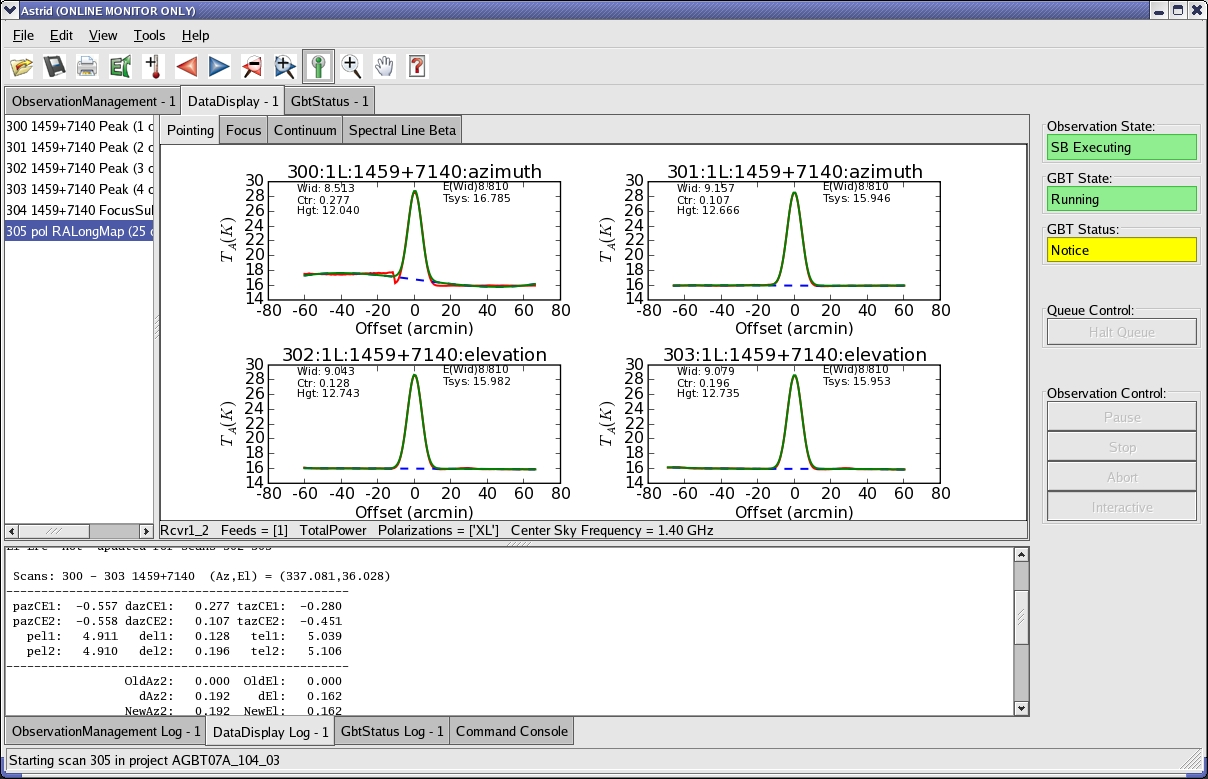
\includegraphics[width=0.6\linewidth]{AstridDataDisplayTabPointing.jpg}
\caption[The Pointing subtab of the Astrid Data Display]
{The Pointing subtab of the \gls{Astrid} Data Display. 
\label{fig:astridpointing} }
\end{center}
\end{figure}

The focus scan data will appear under the Focus Tab; see Figure~\ref{fig:astridfocus}.
Again, if \dq{Online} the data will be processed automatically. They will be calibrated,
have a \gls{baseline} removed and a Gaussian will be fit to the data.  The focus offset
will automatically be sent to the \gls{MC} system.

\begin{figure}[!h]
\begin{center}
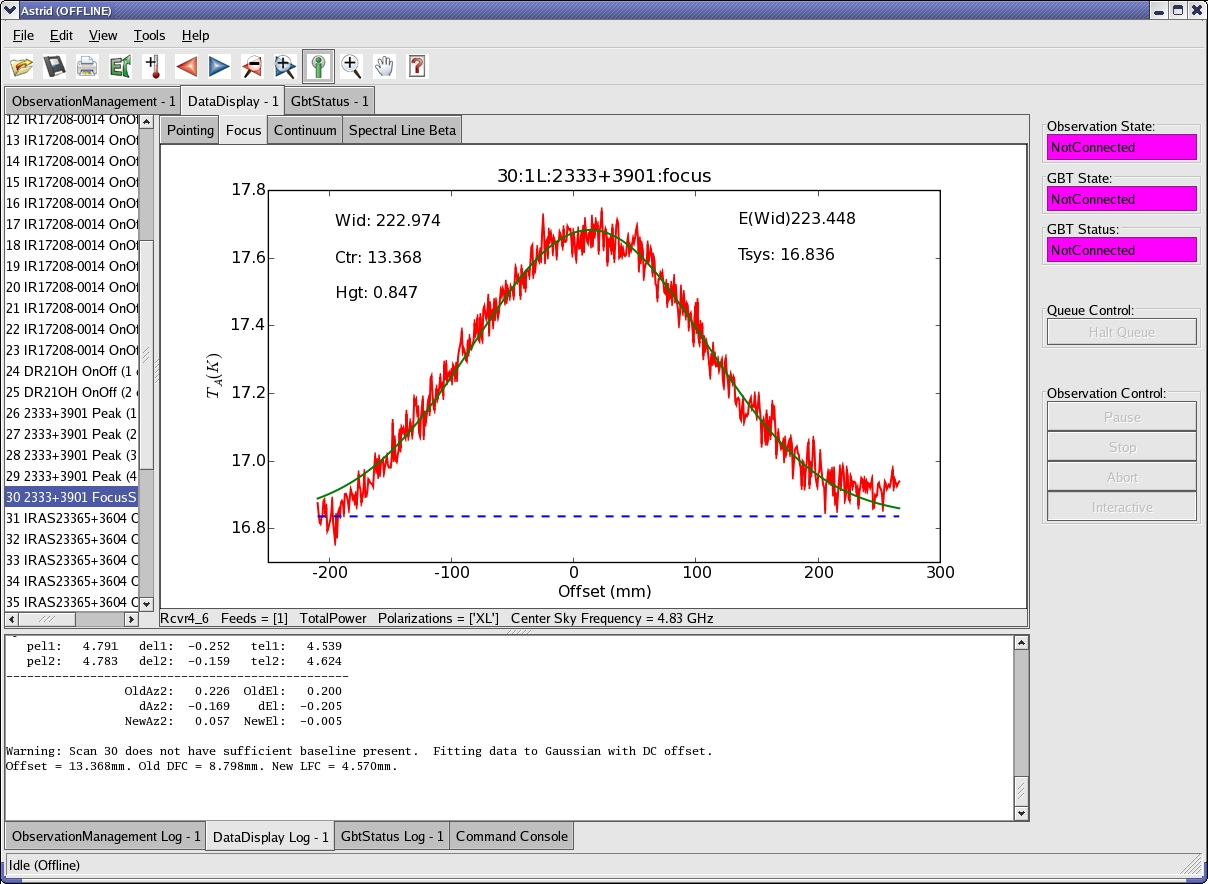
\includegraphics[width=0.6\linewidth]{AstridDataDisplayTabFocus.jpg}
\caption[The Focus subtab of the Astrid Data Display]
{The Focus subtab of the \gls{Astrid} Data Display. 
\label{fig:astridfocus} }
\end{center}
\end{figure}

\noindent The details of pointing and focus observations are described in \S~\ref{sec:utilityscans}.

\newpage

\subsubsection{Fitting Acceptance Options}\label{sec:fittingacceptance}

\gls{GFM} has several levels of determining whether or not the pointing and focus
solutions will be updated in the \gls{MC} system. The expected \gls{FWHM} of the Gaussian
fitted to the observed pointing data as the \gls{GBT} slews across the source should be 
$\sim 748/\nu_{\rm GHz}$\,arc--seconds where $\nu_{\rm GHz}$ is the observing frequency in
GHz.

For a focus scan the resulting data should approximate a Gaussian with a \gls{FWHM} of
$1080\ \nu_{\rm GHz}$, in mm. The default behavior is to asssume that a pointing fit is
bad if the \gls{FWHM} differ from the expected value by more than $30\%$ or if the pointing
correction is more than twice the \gls{FWHM} in magnitude.  The default for a bad focus
scan is if the \gls{FWHM} is more than $30\%$ from the expected value. Users may change
fitting acceptance criteria by: 

\begin{enumerate}[label=\bfseries{Step \arabic*.},leftmargin=*,itemsep=0pt]
\item Select the Pointing or Focus Subtab in the Data Display.
\item Select {\btt Tools}$\rightarrow${\btt Options...} from the drop--down menu.
\item Select the new mode in the \dq{Fitting Acceptance Criteria} tab of the pop--up window.
\item[{\bf NOTE:}] Options must be set independently for both Pointing and Focus
{\bf before} each type of observation in order to take effect.
\end{enumerate}

\noindent \gls{GFM} recognizes the fitting acceptance criteria shown in
Figure~\ref{fig:acceptance} only when \gls{Astrid} is in one of its online modes.
The default setting is to \dq{Automatically accept good fits, automatically reject
bad fits}.  Users may also choose to never apply corrections or interactively accept
bad and/or good fits.  There is also an option to \dq{Accept all automatically} which
can be very dangerous and should only be used by experts.

\vspace{2.5mm}

\noindent\begin{minipage}[t]{0.485\linewidth}
\setlength{\abovecaptionskip}{0pt}\setlength{\belowcaptionskip}{0pt}
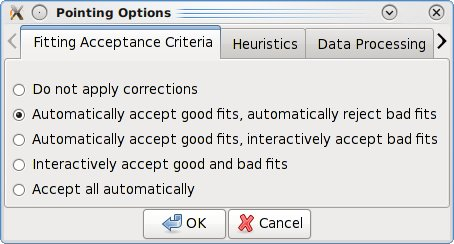
\includegraphics[width=\linewidth]{fittingacceptance.jpg}
\captionof{figure}[Pointing and Focus acceptance pop-up]
{The pop--up menu to change the pointing and focus fitting acceptance criteria. 
\label{fig:acceptance} }
\end{minipage}
\hfill
\begin{minipage}[t]{0.485\linewidth}
\setlength{\abovecaptionskip}{0pt}\setlength{\belowcaptionskip}{0pt}
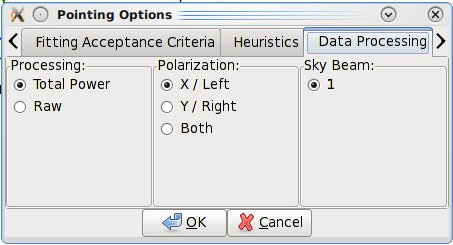
\includegraphics[width=\linewidth]{dataProcessing.jpeg}
\captionof{figure}[Pointing and Focus change fitting pop-up]
{The pop--up menu to change the polarization and calibration used in pointing and
focus fitting. \label{fig:processing} }
\end{minipage}


\subsubsection{Data Processing Options}\label{sec:gfmdataprocessing}

The user may change the data processing strategy, beams, and/or polarizations used 
by \gls{GFM} in reducing pointing or focus scans.  This is not needed typically since the
software picks the proper default settings under normal conditions.  However, for
example, if the X polarization channel is faulty for some reason, one can use the Y
channel instead. This can be done by:

\begin{enumerate}[label=\bfseries{Step \arabic*.},leftmargin=*,%labelindent=\parindent
itemsep=0pt]
\item Select the Pointing or Focus Subtab in the Data Display.
\item Select {\btt Tools}$\rightarrow${\btt Options...} from the drop--down menu.
\item Make new data processing selections in the Data Processing Tab of the pop--up
window (see Figure~\ref{fig:processing}).
\item[{\bf NOTE:}] Options must be set independently for both Pointing and Focus
{\bf before} each type of observation in order to take effect.
\end{enumerate}

\newpage

\subsubsection{Heuristics Options}\label{sec:heuristics}

Heuristics is a generic term used at the \gls{GBT} to quantify the \dq{goodness of fit} of
the pointing and focus data reduction solutions. Based on the known properties of the
\gls{GBT} , parts of the solution, such as the \gls{beamwidth} in pointing data, should
have certain values within measurement errors.  The Heuristics define how large these
errors can be. The user may change the Heuristics by: 

\begin{enumerate}[label=\bfseries{Step \arabic*.},leftmargin=*,
itemsep=0pt]
\item Select the Pointing or Focus Subtab in the Data Display.
\item Select {\btt Tools}$\rightarrow${\btt Options...} from the drop--down menu.
\item Select the new mode in the Heuristics tab of the pop--up window
(see Figure~\ref{fig:heuristic}).
\item[{\bf NOTE:}] Options must be set independently for both Pointing and Focus
{\bf before} each type of observation in order to take effect.
\end{enumerate}

\gls{GFM} allows the observer to switch between \dq{standard}, \dq{relaxed}, and
\dq{user-defined} heuristics.  The \dq{standard} and \dq{relaxed} heuristic values are
predefined and cannot be changed by the user.  Under normal observing conditions the
observer should expect to use the \dq{standard} values.  Under marginal weather
conditions and/or high frequency observations \dq{relaxed} heuristics may be appropriate.
The \dq{user-defined} heuristic values should only be used by experts.  If you wish to
use \dq{user-defined} heuristics then you should contact your \gls{GBT} support scientist.
The default mode is \dq{standard}.

The \dq{standard} heuristics expect that the fitted Gaussians have a \gls{FWHM}
within $30\%$ of the expected values and that the pointing solution is within
twice the \gls{FWHM} of the nominal location of the source.  For the \dq{relaxed}
heuristics this becomes within $50\%$ of the expected \gls{FWHM} of the Gaussian
fits and three times the \gls{FWHM} for the pointing correction.

\vspace{2.5mm}

\noindent\begin{minipage}[t]{0.45\linewidth}
\setlength{\abovecaptionskip}{0pt}\setlength{\belowcaptionskip}{0pt}
\vspace{0pt}
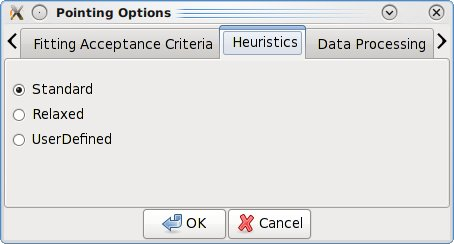
\includegraphics[width=\linewidth]{heuristics.jpg}
\captionof{figure}[Pointing and Focus heuristics pop-up]
{The pop--up menu to change the pointing and focus fitting heuristics.
\label{fig:heuristic} }
\end{minipage}
\hfill
\begin{minipage}[t]{0.45\linewidth}
\setlength{\abovecaptionskip}{0pt}\setlength{\belowcaptionskip}{0pt}
\vspace{0pt}
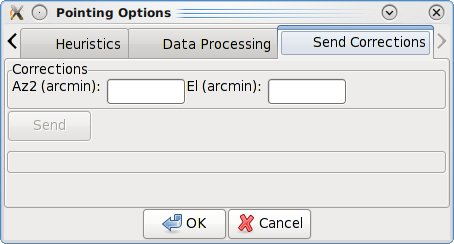
\includegraphics[width=\linewidth]{sendcorrections.jpg}
\captionof{figure}[Send Corrections pop-up]{The pop--up menu to manually send pointing corrections
to the telescope.\label{fig:sendcorrections} }
\end{minipage}

\vspace{-2.5mm}

\subsubsection{Send Corrections}\label{sec:gfmsendcorrections}

For most observations, \gls{GFM} processing produces good fits, and the solutions are
automatically sent to the telescope using the default settings.  However, at high
frequencies (especially \gls{Wband} 68-92 GHz Receiver), fits may fail, and the user may want
to manually send the corrections to the telescope.  The user may tell the operator to
enter a solution, or they can send the corrections themselves using the Send Corrections
tab. Note that corrections show up instantly within the \gls{CLEO} status window
(see \S~\ref{sec:cleo}), but do not take effect until the start of the next scan.
This can be done by:

\begin{enumerate}[label=\bfseries{Step \arabic*.},leftmargin=*,
itemsep=0pt]
\item Select the Pointing or Focus Subtab in the Data Display.
\item Select {\btt Tools}$\rightarrow${\btt Options...} from the drop--down menu.
\item Select the Send Corrections Tab in the pop--up window (if not visible use
arrow button on the right, the Send Corrections tab is farthest to the right)
\item Enter the corrections in the text box, and click \astridbutton{Send} to send the
solutions to the telescope. (see Figure~\ref{fig:sendcorrections}).
\end{enumerate}

\newpage

\subsection{OOF Data Display}\label{sec:oofdatadisplay}

\gls{OOF} is a technique for measuring large-scale errors in the shape of the reflecting
surface by mapping a strong point source both in and out of focus.  The procedure
derives surface corrections which can be sent to the active surface controller to
correct surface errors. The procedure is recommended for high-frequency observing at
frequencies of 30~GHz and higher.

The AutoOOF procedure will obtain three \gls{OTF} maps, each taken at a different focus
position.  Processing will begin automatically upon completion of the third map, the
status of which can be viewed in the progress bar under \dq{AutoOOF Processing Status}
on the right--hand--side of the screen.  Once complete, the result will be displayed
in the \gls{OOF} subtab of the \gls{Astrid} Data Display (see
Figure~\ref{fig:AstridAutoOOF}).

\begin{figure}[!h]
\begin{center}
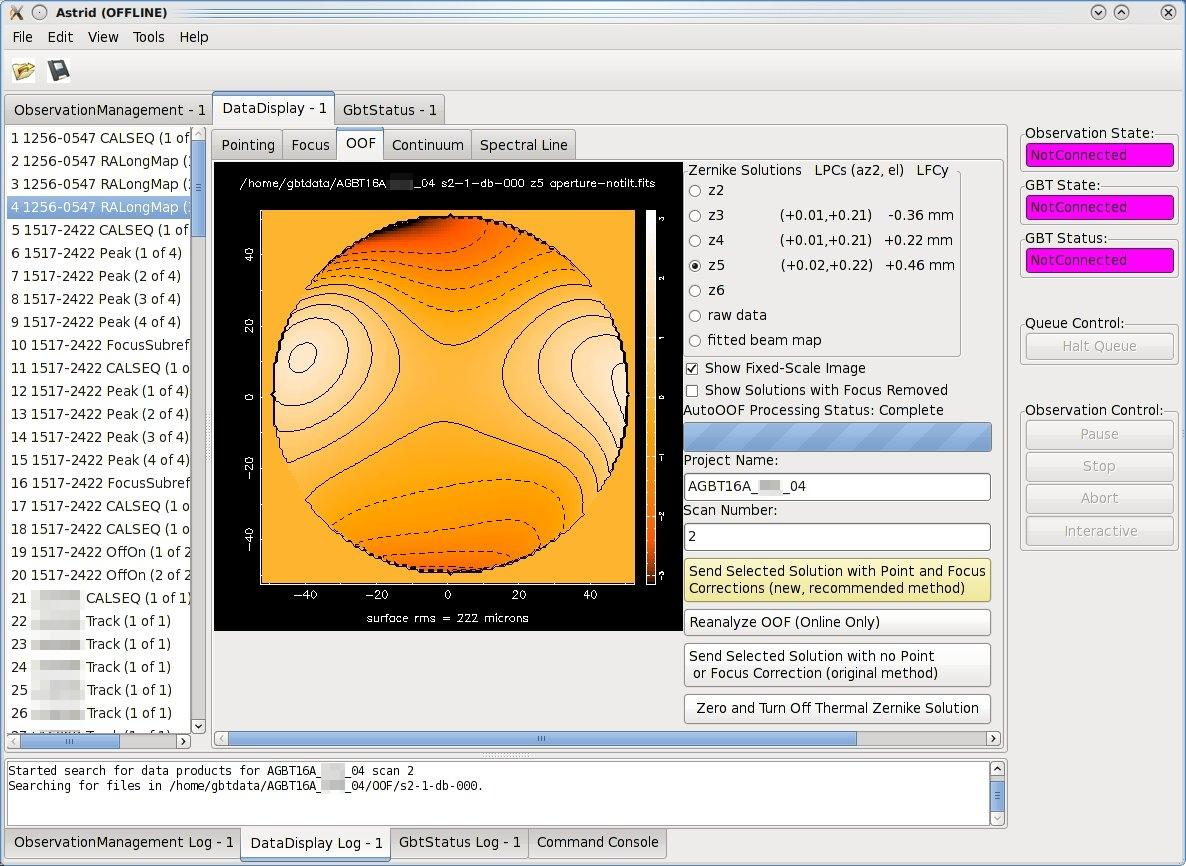
\includegraphics[width=\linewidth]{oof_screen.jpg}
\caption[The OOF subtab of the Astrid Data Display]
{The OOF subtab of the \gls{Astrid} Data Display.\label{fig:AstridAutoOOF} }
\end{center}
\end{figure}

Once processing is complete, the default solution displayed in \gls{Astrid} is the
fifth-order Zernike fit (z5).  The most aggressive fit is z6, while z3 is less
aggressive.  Solutions may be selected and viewed via the radio buttons in the
upper--right section of the screen.  Derived Local Pointing Corrections (LPCs) in
arcminutes, and Local Focus Corrections (LFCy) in millimeters are displayed to the right
of each radio button.  Raw AutoOOF data at each focus position can be viewed as
as a timestream and map by selecting the \dq{raw data} radio button.  The
\dq{fitted beam map} radio button will display fitted beam map images and
reduced $\chi^{2}$ values for the three highest orders of Zernike fits
(z3, z4, and z5 by default).

Solutions must be chosen by the observer and manually sent to the active surface.
Therefore, it is essential that the Zernike fits and raw AutoOOF data are examined
carefully before deciding upon a solution.  Steps for validating and discerning
appropriate solutions be found in the following sections.

\newpage

\subsubsection{AutoOOF Solutions}\label{sec:AutoOOFsolution}

Figure~\ref{fig:OOFsolution} shows examples acceptable and unacceptable
\gls{OOF} solutions.  Good solutions have the following characteristics:

\begin{itemize}[itemsep=0pt]
\item Broad features of less than $\pm 1.5$ radians of phase in early to mid-morning to a
few radians in the afternoon.  Note that you may uncheck \dq{Show Fixed Scale Image} to view
the full data range in the color bar.
\item Surface rms residuals $<$ 400 $\mu$m.
\end{itemize}

\begin{figure}[!h]
\begin{center}
\subfloat[Acceptable OOF solution.\label{fig:goodOOFsolution}]
{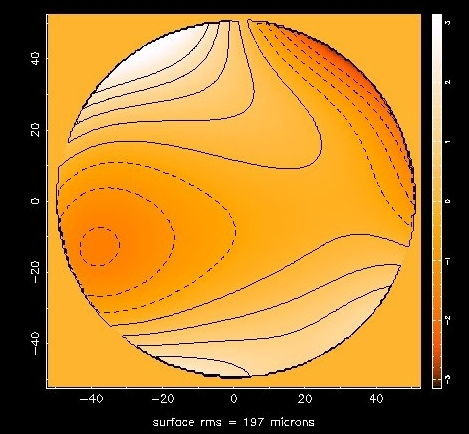
\includegraphics[width=.485\linewidth]{OOFgoodExample.jpg}}
\hfill
\subfloat[Unacceptable OOF solution.\label{fig:badOOFsolution}]
{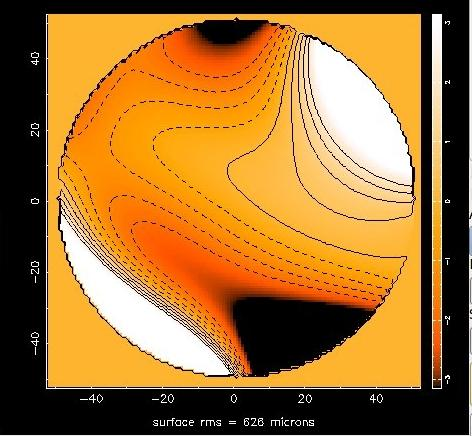
\includegraphics[width=.485\linewidth]{badoof.jpg}}
\caption[Comparison of AutoOOF solutions]
{Figure~\ref{fig:goodOOFsolution} shows broad features ($\pm 1.5$ radians
of phase) with a surface rms of 197 $\mu$m.  Figure~\ref{fig:badOOFsolution} shows
steep contour lines ($\pm 15$ radians of phase) and a surface rms of 626 $\mu$m.
This is likely the result of poor quality raw data and should not be used.} 
\label{fig:OOFsolution}
\end{center}
\end{figure}

%\vspace{-5mm}

\subsubsection{AutoOOF Raw Data}

Although an \gls{OOF} solution may appear to be reasonable (e.g.,
Figure~\ref{fig:goodOOFsolution}) it may also be invalid if it was derived
from a bad set of raw data.  Sending such a solution to the active surface could
degrade performance.  Therefore, observers should always check the quality of the
raw AutoOOF data in order to determine whether their derived solutions are valid.
For a set of raw data to be considered valid, it should show the following
characteristics:

\begin{itemize}[itemsep=0pt]
\item Clear detections of the source in the raw data timestream at all focus positions.
\item Symmetrical left/right positive/negative pattern in all three raw data images.
\item Smooth features in all three raw data images.  Sharp edges or stripes indicate
hardware/software glitches or excessive winds.
\end{itemize}

The AutoOOF raw data can be viewed by selecting the \dq{raw data} radio button in the
upper--right section of the OOF Subtab of the Data Display. Each column represents one focus
position.  The top row is the raw timestram data from the receiver, the second row
has the baselines removed, and the bottom row shows the corresponding beam maps.
See Figure~\ref{fig:rawOOFdata} for a comparison of acceptable and unacceptable
raw AutoOOF data.

\newpage

\begin{figure}[!h]
\begin{center}
\subfloat[A plot of the raw \gls{OOF} data on a fairly clean \gls{Kaband}/\gls{CCB} dataset.
\label{fig:goodOOFdata}]
{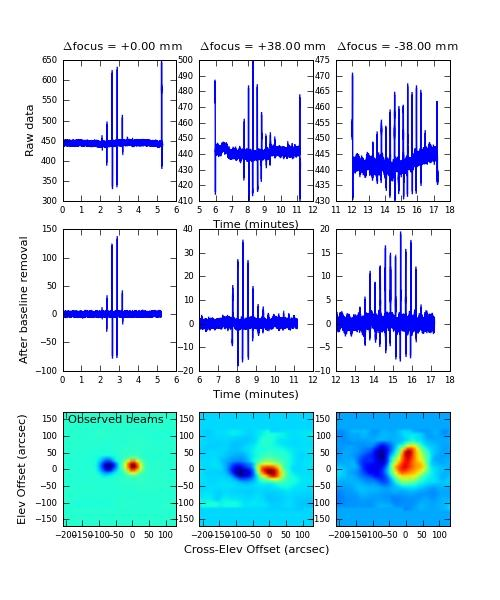
\includegraphics[width=.485\linewidth]{goodOOF.jpg}}
\hfill
\subfloat[A plot of raw \gls{OOF} data on a source which is too faint.
\label{fig:badOOFdata}]
{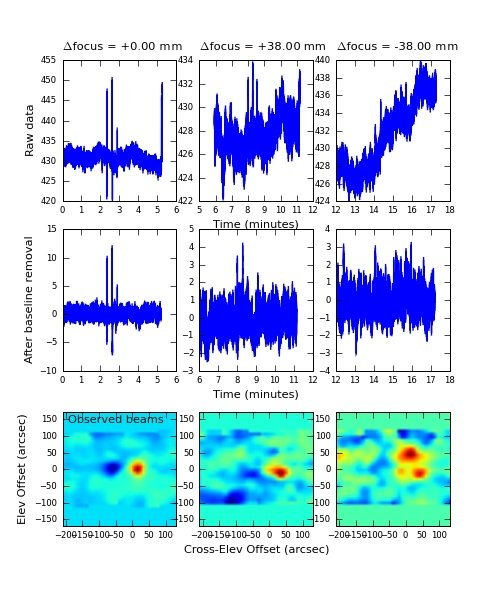
\includegraphics[width=.485\linewidth]{badOOF.jpg}}
\caption[Comparison of AutoOOF raw data]
{A comparison of acceptable and unacceptable AutoOOF raw data.}
\label{fig:rawOOFdata}
\end{center}
\end{figure}


\subsubsection{Selecting the Zernike order to fit}

By default, AutoOOF will halt processing after the fifth-order Zernike (z5) solution
has been computed. The z5 solution is suitable for most conditions and is generally what
observers should expect to use. A more agressive sixth-order (z6) fit may also be
derived at the cost of a few additional minutes of processing time.  This is usually
unnecessary and should only be done on bright calibrators under favorable weather
conditions. See \S~\ref{sec:OOFprocessing} for information on how to change the maximum
order of fit to process.

Occasionally, it may be necessary to occasionally drop to a lower order of fit if the
following features are seen:

\begin{itemize}[leftmargin=*]
\item {\bf Large excursions} over a significant area of the dish edge in the \gls{OOF}
solution.
\item {\bf Regularly spaced features} around the circumference of the dish at higher
order fits in the \gls{OOF} solution.
\item {\bf Anomalous values in the pointing/focus \gls{LPC}/\glspl{LFC}} for one
particular solution, or a significant jump in \glspl{LPC} above a certain Zernike fit
order.  For example, if the focus (LPCy) values for the z3--z4 solutions are around $-3mm$,
then abruptly jump to $+10mm$ for the z5 solution, then it would be prudent to assume that
some or all of the solutions may be invalid.  It may be possible to determine which solutions
are valid by examining the fitted beam maps for obvious artifacts or deviations from the
observed beams (see Figure~\ref{fig:fittedoofmap}).
\end{itemize}

\newpage

\begin{center}
\noindent\begin{minipage}[t]{0.48\linewidth}
\vspace{0pt}
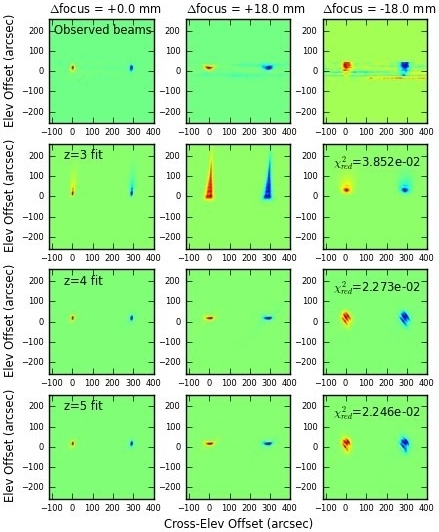
\includegraphics[width=\linewidth]{fittedoofmap_crop.jpg}
\end{minipage}
\hspace{0.025\linewidth}
\begin{minipage}[t]{0.36\linewidth}
\vspace{0pt}
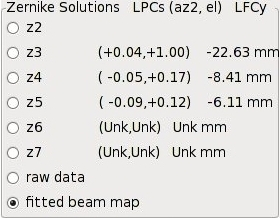
\includegraphics[width=\linewidth]{fittedoofmap_lpc.jpg}
\setlength{\abovecaptionskip}{0pt}\setlength{\belowcaptionskip}{0pt}
\captionof{figure}[AutoOOF fitted beam maps indicating a bad solution]
{The AutoOOF fitted beam maps (left). The observed beams are plotted on the top row
with the z3, z4 and z5 fits to the observed beams plotted below. The z3
solution (2$^{\text{nd}}$ row down) shows an obvious artifact and should not be used.
Also note the significant jump in \glspl{LPC} and the \gls{LFC} between the z3 and
z4 solutions (above).
\label{fig:fittedoofmap}}
\end{minipage}
\end{center}

\vspace{-2.5mm}
\subsubsection{Sending a Solution to the Active Surface}
\vspace{-2.5mm}

When you are ready to accept the solution being displayed it will need to be manually
sent to the active surface.  It is recommended that when sending the solutions, you use
the yellow button labeled
\astridyellowbutton{Send Selected Solution with Point and Focus Corrections}.
If you use this option, you do not have to perform a Peak or Focus after an AutoOOF.
It is still good practice to Peak and Focus at the beginning of your observing session
unless you are using the \gls{Wband} 68--92~GHz recevier (see Chapter~\ref{chap:wband}).
Subsequent pointing and focus corrections may be computed via AutoOOF.

Many high frequency observers will perform Peak scans immediately following
an AutoOOF to verify the surface solution (see \S~\ref{sec:oof_strategy}).
If the solution is satisfactory the \glspl{LPC} and \gls{LFC} from Peak/Focus
scans should agree with values from the \gls{OOF} solution, there should be no significant
sidelobes visible in the peak scans, and Peak scans should also yield the expected
beam \gls{FWHM}. If in doubt, you may disable \gls{OOF} corrections by pressing
\astridbutton{Zero and Turn Off Thernal Zernike Solution} in order to compare
Peak scans with and without \gls{OOF} corrections.

\subsubsection{OOF Processing Options}\label{sec:OOFprocessing}
\vspace{-2.5mm}

Deriving the sixth-order Zernike (z6) solution will require a few additional minutes of
processing time and for the user to manually change the maximum order of fit to process
in the following way:

\begin{center}
\noindent\begin{minipage}[t]{0.19\linewidth}
\setlength{\abovecaptionskip}{0pt}
\setlength{\belowcaptionskip}{0pt}
\vspace{0pt}
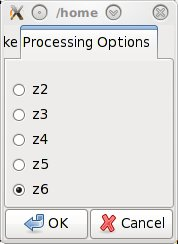
\includegraphics[width=0.73\linewidth]{OOFprocessing_options.jpg}
\captionof{figure}[OOF Processing Options]
{OOF Processing Options.
\label{fig:OOFprocessing}}
\end{minipage}
\begin{minipage}[t]{0.7\linewidth}
\vspace{0pt}
\begin{enumerate}[label=\bfseries{Step \arabic*.},leftmargin=*,itemsep=0pt]
\item Select the OOF Subtab of the Data Display.
\item Select {\btt Tools}$\rightarrow${\btt Options...} from the drop--down menu.
\item Select the maximum order of fit to process from the \newline
\dq{Processing Options} tab of the pop--up window (Figure~\ref{fig:OOFprocessing}).
\item[{\bf NOTE:}] All changes must be made {\bf before submitting the \gls{SB}}
containing the \textbf{\textcolor{pythonKeywords}{AutoOOF}()} function in order to take
effect.  You may also repeat processing after making any changes by pressing
\astridbutton{Reanalyze OOF (Online Only)}.
\end{enumerate}
\end{minipage}
\end{center}

%%%%%%%%%%%%%%%%%%%%%%%%%%%%%%%%%%%%%%%%%%%%%%%%%%%%%%%%%%%%%%%%%%%%%%%%%%%%%%%%%%%%%

\newpage

\subsection{Continuum Data Display}

Continuum data taken with the \gls{GBT} that are not part of pointing and focus
scans will show up in plots under the Continuum Tab
(see Figure~\ref{fig:astridcontinuum}).  This will show the uncalibrated continuum
data as a function of time only.

\begin{figure}[!h]
\begin{center}
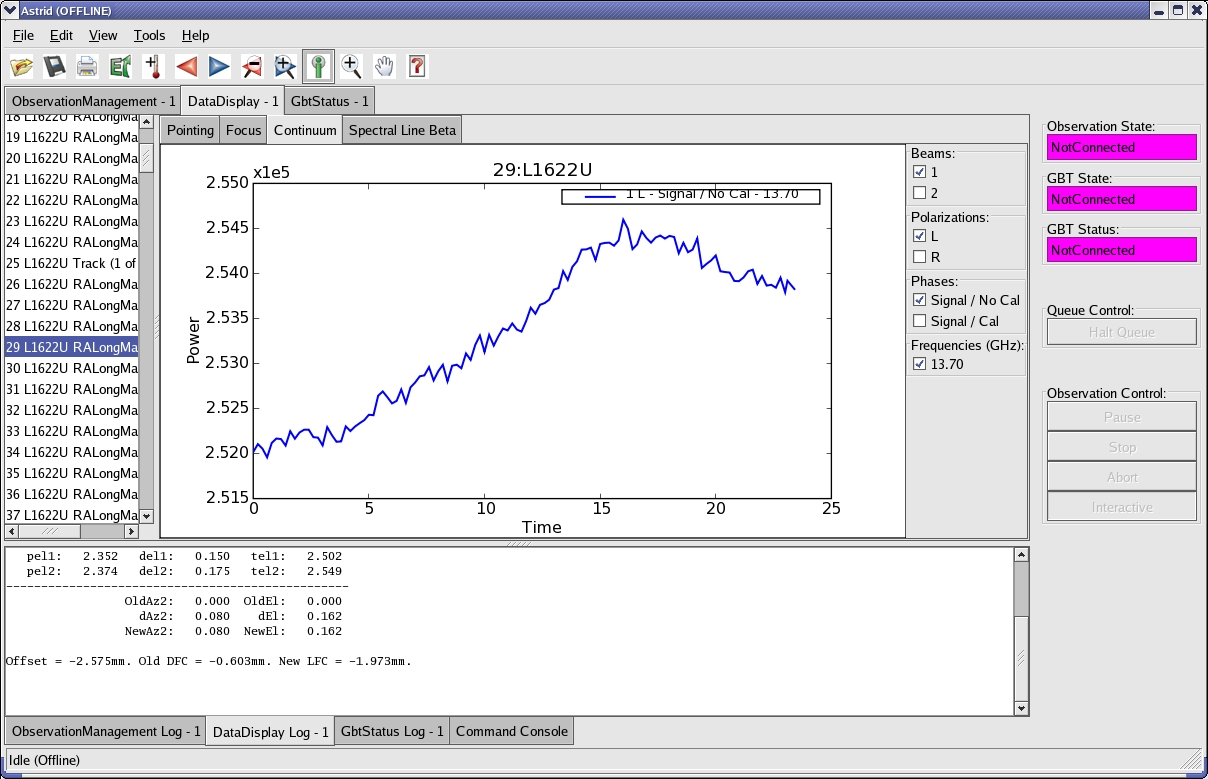
\includegraphics[width=0.9\linewidth]{AstridDataDisplayTabContinuum.jpg}
\caption[The Continuum subtab of the Astrid Data Display]
{The Continuum subtab of the \gls{Astrid} Data Display.\label{fig:astridcontinuum} }
\end{center}
\end{figure}

\vspace{-5mm}

\subsection{Spectral Data Display}\label{sec:spectral_data_display}

The Spectral Line Display was a tool originally designed for browsing the previous
\gls{GBT} Spectrometer spectral line data.  Although this tool can provide limited
\gls{VEGAS} information, there is a separate, more flexible web-based display intended
for \gls{VEGAS}. See \S~\ref{sec:vegasdisplay} for more details.

When viewing data online, the most recent integration is plotted automatically.
Individual integrations may be selected and viewed offline. See
Figure~\ref{fig:astridspectralline} for an example of the spectral line data display.
The spectra displayed are raw data and no calibration has been applied to them.
As spectra are plotted, information about each plot is printed in the console window.
Each line is color coded to match the color of that spectrum in the plotting window. In
addition, some of the information for the very first spectra are used to annotate the
plot. The plot title is parsed as project\_name:scan\_number:integration\_number.
For offline usage, the desired integration can be selected either using the up/down arrows,
or by typing in a value in the edit box.

All user interaction for this plugin occurs in the right-hand side options panel. The
check boxes allow selection of spectra to plot via astronomical variables: Beams,
Polarizations, \gls{IF} Numbers, and Phases.
The options panel also includes three buttons and a radio box for plot viewing. The
\dq{Views} radio box offers options for plotting the bandpass vs. Channels or Sky
Frequency. The \astridbutton{Keep Zoom} toggle button will maintain the current zoom, even
as new spectra are plotted. Using the unzoom command (mouse right-click, or via the
tool bar) will return the plot to its original scale. The \astridbutton{Overlay} toggle
button can be used to overplot spectra from different integrations or scans.
Finally, the \astridbutton{Clear} button erases the plot.

\newpage

\begin{figure}[!h]
\begin{center}
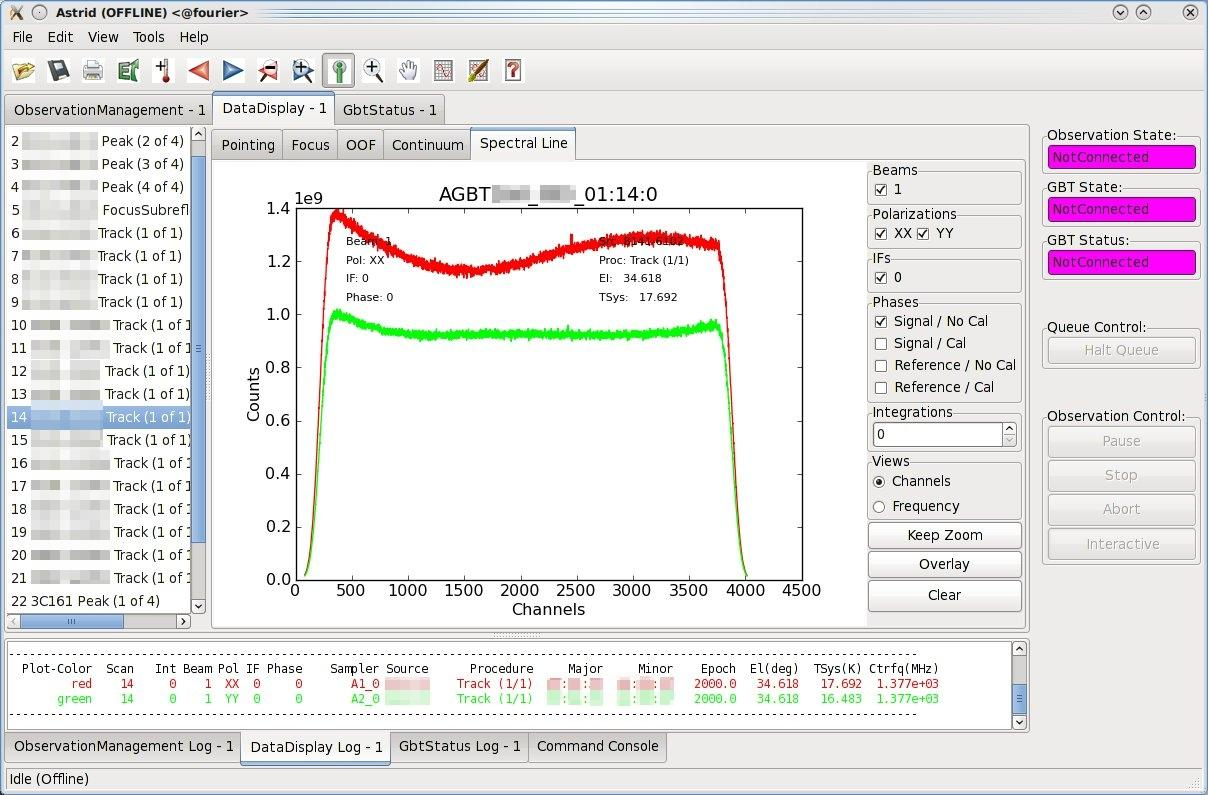
\includegraphics[width=0.9\linewidth]{AstridSpectralDisplay.jpg}
\caption[The Spectral Line subtab of the Astrid Data Display]
{The Spectral Line subtab of the \gls{Astrid} Data Display. 
\label{fig:astridspectralline} }
\end{center}
\end{figure}


\subsection{The Data Display Plotting Panel Toolbar}

The plotting panel toolbar allows user interactions with plots in the display window and
is located near the top of the Astrid Screen.  The following features are available:

\begin{itemize}
\item[
\includegraphics{DTopen.jpg}] {\bf Open:} Allows the user to open a previously
saved session.  This has the same functionality as file $\rightarrow$ open described
in \S~\ref{sec:workingOffline}.
\item[
\includegraphics{DTsave.jpg}] {\bf Save:} Allows the user to save output from the
data display log as a text file.
\item[
\includegraphics{DTprint.jpg}] {\bf Print (DO NOT USE):} Please use the \dq{export}
function instead.
\item[
\includegraphics{DTexport.jpg}] {\bf Export:}  Allows the user to save the figure
displayed in the plotting panel to a file.  The name must have an extension of either
.png, .ps or .eps.
\item[
\includegraphics{DTunfreeze.jpg}] {\bf Unfreeze:} Not applicable to Astrid general
use. Unfreezes the processing of commands via the command line and intended for use in
conjunction with the \dq{freeze} command.
\item[
\includegraphics{DTundo.jpg}] {\bf Undo:} Undoes your last command.
\item[
\includegraphics{DTredo.jpg}] {\bf Redo:} Redoes your last command.
\item[
\includegraphics{DTunzoom.jpg}] {\bf Unzoom:} Undoes a previously executed zoom.
\item[
\includegraphics{DTrezoom.jpg}] {\bf Rezoom:} Redoes a previously executed zoom.
\item[
\includegraphics{DTinfo.jpg}] {\bf Info Tool:} Selecting the info tool allows the
user to use the mouse pointer to focus in/out among the available subplots (e.g., peak
scans). Left-clicking the mouse brings a subplot into focus (hiding the other subplots).
Right-clicking the mouse on the focused plot will show all subplots. If there is only
one subplot, the info tool simply displays the mouse xy coordinates.
\item[
\includegraphics{DTzoom.jpg}] {\bf Zoom Tool:} Selecting the zoom tool allows the
user to use the mouse pointer for zooming in on a particular area of the plot.
Left-clicking the mouse will zoom in. Right-clicking the mouse will zoom out.
\item[
\includegraphics{DTpan.jpg}] {\bf Pan Tool:} Allows the user to use the mouse
pointer to pan around the selected subplot.  Left-clicking the mouse and holding the left
button down will pan around the subplot. Right-clicking restores the original view.
\item[
\includegraphics{DTgrid.jpg}] {\bf Grid Tool:} Turns on the plot grid.
\item[
\includegraphics{DTplotedit.jpg}] {\bf Plot Edit Tool:} Allows the user to edit
plot labels, colors, and title. Clicking on "Advanced Options" brings up an additional
dialog which contains options for transparency, legend placement, and ordering of plots.
Colors may be entered as hex codes or selected by clicking on the colored button to the
right of the text field. Plots can only be reordered within their subplot - i.e., Y1
lines will always be below Y2 lines. Legend location can be specified with simple
strings (e.g., "upper right") or coordinates 0-1 along the plot edges. If a string is
chosen it will be used in place of any coordinates.
\item[
\includegraphics{DTusermanual.jpg}] {\bf User Manual:} Displays the DEAP user
manual.

\end{itemize}


\subsection{Use of Plotting Capabilities}

A User Manual is available at
\htmladdnormallink{http://deap.sourceforge.net/help/index.html}
{http://deap.sourceforge.net/help/index.html}
that describes all the plotting functionality available in \gls{GFM}. There is also a
plotting Tutorial that illustrates the plotting capabilities by example which is
available at
\htmladdnormallink{http://deap.sourceforge.net/tutorial/index.html}
{http://deap.sourceforge.net/tutorial/index.html}.


%++++++++++++++++++++++++++++++++++++++++++++++++++++++++++++++++++++++++++++
\newpage

\section{The CLEO Utilities}\label{sec:cleo}

The \glsfirst{CLEO} system provides a large number of utilities for monitoring
and controlling the GBT hardware systems. Some of these are quite useful for observers,
although most are intended for expert users and \gls{GBT} staff.

Useful help messages pop up when you hover the mouse over any \gls{CLEO} widget for a
few seconds.  Documentation is also available on the following web pages, but is somewhat
out of date, so its best to consult your \gls{GBT} \dq{friend} for details.
\begin{itemize}
\item \htmladdnormallink
{http://www.gb.nrao.edu/$\sim$rmaddale/GBT/CLEOManual/index.html}
{http://www.gb.nrao.edu/~rmaddale/GBT/CLEOManual/index.html}
\item \htmladdnormallink
{http://www.gb.nrao.edu/$\sim$rmaddale/GBT/CLEOManual/tableofcontents.html}
{http://www.gb.nrao.edu/~rmaddale/GBT/CLEOManual/tableofcontents.html}.
\end{itemize}

\noindent The following section describes just a few \gls{CLEO} utilities that are
useful for observers.

\subsection{Starting CLEO}

\noindent\begin{minipage}[b]{0.29\linewidth}
\vspace{0pt}
\captionsetup{
  justification=raggedright,
  singlelinecheck=false
}
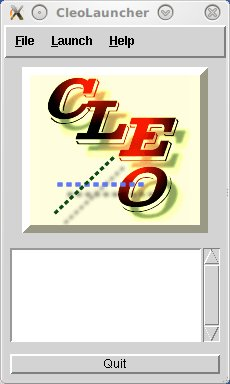
\includegraphics[width=\linewidth]{cleoLauncher.jpg}
\captionof{figure}[The Cleo Launcher]
{The Cleo Launcher.
\label{fig:cleoLauncher}}
\end{minipage}
\hfill
\noindent \begin{minipage}[b]{0.685\linewidth}
\vspace{0pt}
\includegraphics[width=\linewidth]{CLEOtalkAndDraw.jpg}
\captionof{figure}[CLEO Talk and Draw]
{The \gls{CLEO} Talk and Draw application launched as a tab of the Cleo Container.
\label{fig:CLEOtalkanddraw}}
\end{minipage}

To start \gls{CLEO}, log in to any Linux workstation in Green Bank, open a terminal 
window, and type {\tt cleo}.  A \dq{Cleo Launcher} window will appear
(see Figure~\ref{fig:cleoLauncher}).  Click on the {\btt \underline{L}aunch} menu
to get a list of programs that can be run.  Remote observers working via \gls{VNC} may
prefer to use \dq{Cleo Container} which launches and displays \gls{CLEO} applications
as tabs within a single window.  Cleo Container can be opened from the terminal by typing 
{\tt cleo cleocontainer} or from the Cleo Launcher via\\
{\btt \underline{L}aunch} $\rightarrow$ {\btt \underline{C}leo Container...}

\newpage

\subsection{Talk and Draw}\label{sec:talkanddraw}
{\btt \underline{L}aunch} $\rightarrow$ {\btt \underline{O}bserver
Tools} $\rightarrow$ {\btt Talk and Dra\underline{w}}

Launching \dq{Talk and Draw} will open a window that allows communication
with all other users of the same application including the \gls{GBT} operator
(see Figure~\ref{fig:CLEOtalkanddraw}). Messages typed in the white text box
near the bottom of the screen will become visible to other users after pressing
the \dq{Enter} key.

Users may also create private groups via the \cleobutton{Create New Group} button and
inviting other users to join.  The private session will be accessible through a new
tab next to the default \dq{AllUsers} tab.  Users may then send messages within
their newly created group or to \dq{AllUsers} (including the operator) by selecting
the relevant tab and entering a message.



\subsection{Scheduler and Skyview}\label{sec:cleo_scheduler}
{\btt \underline{L}aunch} $\rightarrow$ {\btt \underline{O}bserver
Tools} $\rightarrow$ {\btt Sc\underline{h}eduler \& Skyview...}

This displays a plot of the sky in Az/El coordinates as viewed from Green Bank as
shown in Figure~\ref{fig:CLEOskyview}.   One can import a catalog of source positions
to be displayed, or display one of the lists of standard calibration sources.
By default it displays solar system objects. For example, to display sources listed in
the standard \gls{Astrid} \dq{xband\_pointing} catalog press

\begin{itemize}[leftmargin=*]
\item \cleobutton{Catalog...}$\rightarrow$\cleobutton{Add/Select/DeSelect Catalogs...}%
$\rightarrow$\cleobutton{xband\_pointing}$\rightarrow$\cleobutton{Apply}$\rightarrow$\cleobutton{OK}
\end{itemize}

If one selects \cleobutton{Schedule} (button at upper right), one may enter a date and time
and display the sky for that time.  It shows the corresponding \gls{LST}, and moving
the cursor on the plot displays the RA/Dec and Az/EL under the cursor. This is very
useful for planning observations. There is also a \cleobutton{Real Time} option in which the
location of objects and the direction the \gls{GBT} is pointed are displayed for the
current time.

\begin{figure}[!h]
\setlength{\abovecaptionskip}{0pt}\setlength{\belowcaptionskip}{0pt}
\begin{center}
\includegraphics[width=0.6\linewidth]{CLEOscheduler.jpg}
\caption[CLEO Scheduler \& Skyview]
{The \gls{CLEO} Scheduler \& Skyview application.
\label{fig:CLEOskyview}}
\end{center}
\end{figure}
\newpage

\subsection{Status}
{\btt \underline{L}aunch} $\rightarrow$ {\btt S\underline{t}atus...}

This displays the status of many \gls{GBT} systems all on one screen as shown in
Figure~\ref{fig:CLEOstatus}. While very useful, it is not recommended for use remotely because it 
is a heavy user of computing resources.  For remote observing, it is
recommended to use the Astrid GbtStatus display (See Section~\ref{sec:astridstatus}).

\begin{figure}[!h]
\begin{center}
\includegraphics[width=0.7\linewidth]{CLEOstatus.jpg}
\caption[CLEO Status]
{The \gls{CLEO} Status application.
\label{fig:CLEOstatus}}
\end{center}
\end{figure}

\vspace{-1cm}

\subsection{Messages}
{\btt \underline{L}aunch} $\rightarrow$ {\btt \underline{M}essages...}

This shows all system status messages as shown in Figure~\ref{fig:CLEOmessages}.
It's often useful to identify problems that might arise with any of the \gls{GBT} devices.

\begin{figure}[!h]
\begin{center}
\includegraphics[width=0.5\linewidth]{CLEOmessages.jpg}
\caption[CLEO Messages]
{The \gls{CLEO} Messages application.
\label{fig:CLEOmessages}}
\end{center}
\end{figure}


%===========================================================================

\newpage

\section {VEGAS Monitoring Tools}\label{sec:vegas_monitoring_tools}

\subsection {The VEGAS Data Display}\label{sec:vegasdisplay}
Observers are urged to use the real-time data display any time they are observing with
\gls{VEGAS} to monitor data quality in real time. The \gls{VEGAS} real-time data display
may be accessed by pointing a web browser to \htmladdnormallink
{http://vegasdisplay.gb.nrao.edu}
{http://vegasdisplay.gb.nrao.edu}
\begin{center}
(This URL is only accessible to machines inside the Green Bank observing network)
\end{center}

\vspace{-2.5mm}

\begin{figure}[!h]
\setlength{\abovecaptionskip}{0pt}\setlength{\belowcaptionskip}{0pt}
\begin{center}
\includegraphics[width=\linewidth]{vegas_display_layers.jpg}
\caption[The VEGAS real-time data display]{The VEGAS real-time data display.
The first level displays data for each \gls{VEGAS} bank, the second level displays data for
each subband of a selected bank, and the third level displays a false color \dq{waterfall}
plot for a single selected subband.
\label{fig:vegas_real_time_display}}
\end{center}
\end{figure}

\vspace{-2.5mm}

\noindent This will bring up a display as shown in the top-left box of
Figure~\ref{fig:vegas_real_time_display} where each plot represents a bank of \gls{VEGAS}.
Subbands (if available) are color coded within each bank.
\begin{itemize}
\item Clicking on the plot for a \gls{VEGAS} bank or the boxes labelled
\dq{A}$\rightarrow$\dq{H} near the top of the screen will dislay total power in counts
vs. frequency for each subband of the selected bank. A maximum of eight subbands will
be displayed in the plots labelled \dq{Window 0$\rightarrow$7}.  If using a single band
mode of \gls{VEGAS}, then only \dq{Window 0} will display a bandpass.
\begin{itemize}
\item Clicking on a subband plot will display a false color \dq{waterfall} plot, building
up integration by integration.  The right hand plot of this new screen will also display
the bandpass of the latest integration.  Note that the waterfall plot will always rebin
data to 512 channels.
\end{itemize}
\end{itemize}


\newpage

\subsection{The VEGAS CLEO screen}\label{sec:vegas_cleo}


This can be launched via {\btt \underline{L}aunch} $\rightarrow$
{\btt \underline{B}ackends} $\rightarrow$ {\btt \underline{V}EGAS...} from the
\gls{CLEO} launcher (see \S~\ref{sec:cleo}). An example of the \gls{VEGAS}
\gls{CLEO} screen is shown in Figure~\ref{fig:vegas_cleo}.

\begin{figure}[!h]
\begin{center}
\includegraphics[width=\linewidth]{vegascleoscreen.jpg}
\caption[]{The VEGAS CLEO Screen \label{fig:vegas_cleo}}
\end{center}
\end{figure}

The \gls{VEGAS} \gls{CLEO} screen follows standard \gls{CLEO} conventions, and is fairly
self-explanatory. As for all backend screens, \gls{IFsys} information for a selected
bank can be displayed by clicking on the blue square to the right of the Bank label.

The \gls{VEGAS} \gls{CLEO} screen can be used to launch the \gls{VEGAS} Data Monitor (described
in the next section) by clicking on the \cleobutton{VEGAS Power Monitor...} button.

\newpage

\subsection{VEGAS Data Monitor}\label{sec:vegasdm}
The \gls{VEGAS} Data Monitor (VEGASDM) provides a real-time display of the current
total power level as measured by the \gls{VEGAS} \glspl{ADC}, as well as a histogram of
the distribution of \gls{ADC} counts.  VEGASDM may be launched by:

\begin{verbatim}
% source /home/gbt/gbt.bash (or .csh)
% VEGASDM
\end{verbatim}

or by clicking the \cleobutton{VEGAS Power Monitor...} button from the \gls{VEGAS} \gls{CLEO} screen.
The VEGASDM display will appear as in Figure~\ref{fig:vegasdm}

\begin{figure}[!h]
\begin{center}
\includegraphics[width=0.85\linewidth]{vegasdatamonitor.jpg}
\caption[]{The VEGAS Data Monitor screen}
\label{fig:vegasdm} 
\end{center}
\end{figure}

VEGASDM has nine tabs, one for each Bank, and one overview tab. If a Bank is
active, the tab label will be green, otherwise it will be red. Each Bank tab
shows whether the Bank is in the running state, and what mode it is in. The
upper plot shows the total power from each polarization as a function of
time, while the lower two plots show the distribution of \gls{ADC} counts for
each polarization. If \gls{VEGAS} is balanced correctly, the \gls{ADC} counts should
be approximately Gaussian, centered around zero, with a full-width half
maximum of approximately 25--50 counts. If the \gls{ADC} counts are very centrally
peaked, there is not enough power going into \gls{VEGAS}, while if the \gls{ADC} counts
have peaks at +/- 127 counts, \gls{VEGAS} is being over-driven.

The final tab of VEGASDM gives an overview plot of the total power for all
eight banks on a single screen.




%\begin{figure}[!h]
%\begin{center}
%\subfloat[z6 fit with a large excursion near the bottom of the dish
%\label{fig:OOFZ6toZ5bad}]
%{\includegraphics[width=.475\linewidth]{OOFZ6toZ5bad.jpg}}
%\hfill
%\subfloat[z5 fit no longer showing the large excursion
%\label{fig:OOFZ6toZ5good}]
%{\includegraphics[width=.475\linewidth]{OOFZ6toZ5good.jpg}}
%\caption[Selecting the z5 AutoOOF solution]
%{An example of using a lower order z5 fit (figure~\ref{fig:OOFZ6toZ5good}) to
%correct for a large excursion ($\pm 5$ radians of phase) seen near the bottom of the dish in the
%z6 fit (figure~\ref{fig:OOFZ6toZ5bad}).  Also note the slight jump in derived focus LPCs
%from approximately -1.8 mm (z2--z5) to -0.5 mm (z6--z7).}
%\label{fig:OOFZ6toZ5correction}
%\end{center}
%\end{figure}

%\begin{figure}[!h]
%\begin{center}
%\subfloat[z7 fit showing repeating features.\label{fig:OOFZ7toZ6bad}]
%{\includegraphics[width=.475\linewidth]{OOFZ7toZ6bad.jpg}}
%\hfill
%\subfloat[z6 fit no longer showing repeating features.\label{fig:OOFZ7toZ6good}]
%{\includegraphics[width=.475\linewidth]{OOFZ7toZ6good.jpg}}
%\caption[Selecting the z6 AutoOOF solution]
%{An example of using a lower order z6 fit (figure~\ref{fig:OOFZ7toZ6good}) to
%correct for the repeating features seen in the z7 fit (figure~\ref{fig:OOFZ7toZ6bad}).}
%\label{fig:OOFZ7toZ6correction}
%\end{center}
%\end{figure}
% Astrid near real time display and cleo utilities
\glsreset{SB}
\chapter{Scheduling Blocks}\label{chap:scripts}

\vspace*{-0.5cm}

At the \gls{GBT}, we use \glspl{SB} to perform astronomical observations. The \gls{SB}
can contain information for configuring the telescope, balancing the \gls{IFsys}, and
other commands to \dq{tweak} the telescope system (observing directives) along with
the commands (scan types) to collect observational data. \gls{Astrid} interprets
\glspl{SB} via Python. Thus \glspl{SB} should follow Python syntax rules (such as
indentation for loops) and can also contain or make use of any Python commands.
Here is an example of a simple \gls{SB}:

\lstinputlisting[language=PythonAstrid,captionpos=b,label={lst:simplesb},caption=
{[A simple Scheduling Block]A simple \gls{SB}}]
{simple.py}

\begin{itemize}[leftmargin=*,itemsep=0pt]
\item {\bfseries{\textcolor{pythonKeywords}{execfile}}}
loads definitions for configuring the \gls{GBT}'s receivers, \gls{IFsys} and backends
for the observations.  This is described in \S~\ref{sec:config}.
\item {\bfseries{\textcolor{pythonKeywords}{Catalog}}}
loads a catalog containing information (such as positions and radial velocity, etc.) on
the sources to observe.  This is described in \S~\ref{sec:catalogs}.
\item {\bfseries{\textcolor{pythonKeywords}{Configure}}}
runs the configuration defined in {\ttfamily{myconfigurations.txt}} to select the
receiver and backend and set switches and frequencies.
This is described in \S~\ref{sec:config}.
\item {\bfseries{\textcolor{pythonKeywords}{Slew}}}
moves the telescope to the desired source (see \S~\ref{sec:scantypes}).
\item {\bfseries{\textcolor{pythonKeywords}{Balance}}}
balances the power levels in the \gls{IFsys} and backend so that they should be in their
linear regime (see \S~\ref{sec:utility}). 
\item {\bfseries{\textcolor{pythonKeywords}{Track}}}
performs and aquires data for the desired observation.  Track and other pre-defined
scans are described in \S~\ref{sec:scantypes}.
\end{itemize}

\newpage


%++++++++++++++++++++++++++++++++++++++++++++++++++++++++++++++++++++++++++++



%============================================================================
\section{Making A Scheduling Block}

{\bf \glsuserii{SB} must be created well prior to your telescope time. 
We suggest that you review \glspl{SB} with your project's contact support scientist.}

\glspl{SB} can be written using \gls{Astrid}'s \dq{Observation Management} Edit subtab
(see \S~\ref{sec:editsubtab}), which contains a simple text editor reminiscent of Notepad
(MS Windows), or you can choose to write your \gls{SB} outside of \gls{Astrid} and use the
\dq{Observation Management} Import facility in \gls{Astrid} to upload it into the database;
see \S~\ref{sec:astridimport} for details.

For the database, you should choose a descriptive name for your \gls{SB}, such as \dq{map\_G11.0}
or \dq{pointfocus}, which will remind you of the science you are trying to accomplish by running
that block. Names such as \dq{test} or \dq{turtle.p} are not descriptive and should be avoided.
The name you choose can be up to 96 characters long, and can contain white spaces, so you may
have an \gls{SB} name that consists of a few words (such as \dq{K-band frequency-switched
spectroscopy}). You do not need to add a suffix to your \gls{SB} name (*.sb or *.py).

%%%%%%%%%%%%%%%%%%%%%%%%%%%%%%%%%%%%%%%%%%%%%%%%%%%%%%%%%%%%%%%%%%%%%%%%%%%%%%

\subsection{Components of a Scheduling Block}

A typical \glsuseri{SB} will include:
\begin{enumerate}[label=\Alph*),itemsep=0pt]
\item A configuration of the system (see \S~\ref{sec:config}).
\item Specification of the sources via a catalog (see \S~\ref{sec:catalogs}).
\item A slew to the source and then balancing the power levels, and maybe other commands
(see \S~\ref{sec:utility}).
\item Observational scan type commands (see \S~\ref{sec:scantypes}).
\end{enumerate}

\noindent In the following sections we discuss each of these components.


%============================================================================
\section{Configuration of the GBT IF System}\label{sec:config}

%****************************************************************************
\subsection{Overview}

The routing of signals through the \gls{GBT} system is controlled by many electronic
switches which eliminate the need to physically change cables by hand.  The \gls{GBT}'s
electronically configurable \gls{IFsys} allows many, and more complicated paths for
the signals to co-exist at all times.  Configuring the \gls{GBT} \gls{IFsys} can
usually be accomplished in under one minute.

\subsection{Defining and Executing A Configuration}\label{sec:config_define}

\noindent Configurations are defined as sets of keyword--value pairs within a single
string variable. To execute a configuration, this variable is passed as an argument
into the {\bfseries{\textcolor{pythonKeywords}{Configure}}()} command in an \gls{SB}.
Configurations may be defined in two ways:

\begin{enumerate}
\item The configuration definition may reside on a text file external to the \gls{SB}.
It can then loaded into the \gls{SB} via the
{\bfseries{\textcolor{pythonKeywords}{execfile}()}} command
(see script~\ref{lst:config_loaded}).
\item The configuration may be explicitly defined within the \gls{SB}
(see script~\ref{lst:config_declared}).
\end{enumerate}

\newpage

We usually recommend that configuration definitions reside on text files external to
the \gls{SB}. This allows for configurations to be changed on the file without the
need to re-validate and re-save the \gls{SB} (see \S~\ref{sec:validation}). It also
allows for simple \glspl{SB} without clutter.  Note that you should always use
{\bfseries{\textcolor{pythonKeywords}{execfile}}} rather than
{\bfseries{\textcolor{pythonKeywords}{import}}}, as
{\bfseries{\textcolor{pythonKeywords}{import}}} will not reread the file and miss any
changes that you may have made.

Explicitly defining configurations within \glspl{SB} allows users to easily
edit and view their configuration from \gls{Astrid}.  If this method is chosen, users
\textbf{must} re-validate and re-save the \gls{SB} if any changes are made.  Examples
of both methods can be seen in scripts~\ref{lst:config_loaded} and
\ref{lst:config_declared}.

If using multiple configurations, it is recommended that you define them all in one
text file and load them into the \gls{SB} via a single
{\bfseries{\textcolor{pythonKeywords}{execfile}}} command. You may then use
{\bfseries{\textcolor{pythonKeywords}{Configure}}()} to execute each configuration
as necessary.

\noindent\begin{minipage}[t]{0.58\linewidth}
\lstinputlisting[captionpos=b,frame=single,framerule=1pt,language=PythonAstrid,
caption={[Basic configuration syntax]
A text file containing an example of basic configuration syntax.
},label={lst:config_syntax}]
{syntax.py}
\end{minipage}
\hfill
\begin{minipage}[t]{0.38\linewidth}
\lstinputlisting[language=PythonAstrid,captionpos=b,frame=single,
backgroundcolor=\color{sbBackground},framerule=1pt,
caption={[Loading a configuration with execfile()]
An \gls{SB} using
{\bfseries{\textcolor{pythonKeywords}{execfile}}()} to load
the contents of Script~\ref{lst:config_syntax} into \gls{Astrid}.
\dq{myconfiguration} can then be used as an argument to
{\bfseries{\textcolor{pythonKeywords}{Configure}}()} to configure the system.},
label={lst:config_loaded}]
{config_loaded.py}
\end{minipage}

\lstinputlisting[language=PythonAstrid,captionpos=b,frame=single,framerule=1pt,
backgroundcolor=\color{sbBackground},
caption={[Explicitly defining the configuration in a Scheduling Block]
An \gls{SB} that explicitly defines all configuration keywords within
triple quotes as the parameter \dq{myconfiguration}.  This parameter is then used as
an argument to {\bfseries{\textcolor{pythonKeywords}{Configure}}()} in order to configure
the system. This \gls{SB} will perform exactly the same function as the
text file and \gls{SB} shown in Scripts~\ref{lst:config_syntax} and~\ref{lst:config_loaded}.},
label={lst:config_declared}]
{config_declared.py}

\subsection{Basic Configuration Syntax}
An example of the basic configuration syntax is shown in
scripts~\ref{lst:config_syntax} and~\ref{lst:config_declared}.
Configurations are passed into {\bfseries{\textcolor{pythonKeywords}{Configure}}()} as
a string argument.  For each configuration, all keywords and values
(\S~\ref{sec:keywords}) exist as line separated keyword=value pairs,
all enclosed within a single set of triple-quotes.

\newpage

%****************************************************************************
\subsection{Example Configurations}\label{sec:examples}

The best way to learn about how to define and perform configurations is through 
examples.  Keywords available for use in a configuration definition will be 
discussed in \S~\ref{sec:keywords} and all examples have been placed in the directory,

\begin{verbatim}
/home/astro-util/projects/GBTog_examples/configs/
\end{verbatim}

%-----------------------------------------------------------------------------
\vspace*{-0.5cm}
\topic{Continuum Observations}

\lstinputlisting[language=PythonAstrid,captionpos=b,frame=single,framerule=1pt,
caption={[An example continuum configuration]
An example continuum configuration.},
label={lst:continuumconfig}]
{continuum_config.py}
\noindent
The above configuration definition (script~\ref{lst:continuumconfig}) has been given
the name \sq{continuum\_config} and can be used for pointing and focusing observations
or for continuum mapping.  We have configured for the following:


\begin{itemize}
\item \Gls{tpower}, continuum observations [obstype=\sq{Continuum}; swmode=\sq{tp};
swtype=\sq{none}].
\item The  single beam \gls{Lband} (1 to 2~GHz) receiver
[receiver=\sq{Rcvr1\_2}; beam=\sq{1}]
\item The \gls{DCR} as the backend detector [backend=\sq{DCR}]
\item {Take data using a single band centered on 1400~MHz with a 80~MHz bandwidth
      \newline [nwin=1; restfreq=1400; bandwidth=80]}
\item Go through a full switching cycle in 0.2~seconds [swper=0.2]
\item Record data with the \gls{DCR} every 0.2~seconds [tint=0.2]
\item Disable doppler tracking for continuum observations [vframe=\sq{topo};
vdef=\sq{Radio}].
\item Use a low-power \gls{noiseDiode} [noisecal=\sq{lo}]
\item Linear polarization [pol=\sq{Linear}]
\end{itemize}

%-----------------------------------------------------------------------------
\newpage

\topic{Spectral Line, Frequency Switching Observations}

\lstinputlisting[language=PythonAstrid,captionpos=b,frame=single,framerule=1pt,
caption={[An example frequency switched, spectral line configuration]
An example frequency switched, spectral line configuration.},
label={lst:fsconfig}]
{fs_config.py}

\noindent The above example (script~\ref{lst:fsconfig}) will configure for the
following:
\begin{itemize}
\item \Gls{fsw}, spectral line observations [obstype=\sq{Spectroscopy}; swmode=\sq{sp};
swtype=\sq{fsw}].
\item The single beam \gls{Lband} (1 to 2~GHz) receiver
[receiver=\sq{Rcvr1\_2}]. Note that not specifying \sq{beam} defaults to [beam=\sq{1}].
\item \gls{VEGAS} as the backend detector using linear polarization without
cross-polarization products [backend=\sq{VEGAS}; pol=\sq{Linear}].
\item Take data using a single band using \gls{VEGAS} mode 11
(see Table~\ref{tab:vegas_modes}) defined by a 23.44~MHz bandwidth, 65536 channels,
and one band per spectrometer. [bandwidth=23.44; nchan=65536; vegas.subband=1],
centered on 1420~MHz [restfreq=1420].
\item Go through a full switching cycle in 2~seconds [swper=2.0]. Over one cycle, the
\gls{fsw} states will be centered on the line, and then be shifted by -5~MHz
[swfreq=0,-5.0].
\item Record data with \gls{VEGAS} every 10~seconds [tint=10]
\item Doppler track the spectral line with the rest frequency 1420~MHz in the commonly
used Local Standard of Rest velocity with the radio definition of Doppler tracking
[vframe=\sq{lsrk}; vdef=\sq{Radio}].
\item Use a low-power \gls{noiseDiode} [noisecal=\sq{lo}]
\end{itemize}
\newpage

%-----------------------------------------------------------------------------
\topic{Multiple Spectral Lines, Total Power Observations}

\lstinputlisting[language=PythonAstrid,captionpos=b,frame=single,framerule=1pt,
caption={[An example total power, spectral line configuration]
An example total power, spectral line configuration.},
label={lst:tpconfig}]
{tp_config.py}

\noindent The above example (script~\ref{lst:tpconfig}) will configure for the
following:
\begin{itemize}
\item \Gls{tpower}, spectral line observations [obstype=\sq{Spectroscopy};
swmode=\sq{tp}; swtype=\sq{none}].
\item The single beam \gls{Xband} (8 to 10~GHz) receiver. [receiver=\sq{Rcvr8\_10}].
Note that not specifying \sq{beam} defaults to [beam=\sq{1}].
\item \gls{VEGAS} as the backend detector using circular polarization without
cross-polarization products [backend=\sq{VEGAS}; pol=\sq{Circular}].
\item Mode 21 of \gls{VEGAS} (see Table~\ref{tab:vegas_modes}).  This mode is defined
by a bandwidth of 23.44~Mhz, 8192 spectral channels in the eight subband mode of
\gls{VEGAS} [bandwidth=23.44; nchan=8192].  Note that not specifying \sq{vegas.subband}
for a bandwidth of 23.44~MHz will default to vegas.subband=8.
\item 9 spectral windows, each of which centered on one of the 9 frequencies (in MHz)
listed under restfreq [restfreq=9816.867, 9487.824, 9173.323, ....].
\item Go through a full switching cycle in 1~second [swper=1.0] and record data with
\gls{VEGAS} every 30~seconds [tint=30].
\item Doppler track the spectral line with the rest frequency 8873.1~MHz
[dopplertrackfreq=8873.1] in the commonly used Local Standard of Rest velocity
[vframe=\sq{lsrk}] with the radio definition of Doppler tracking [vdef=\sq{Radio}].
\item Use a low-power \gls{noiseDiode} [noisecal=\sq{lo}].
\end{itemize}

\newpage
%-----------------------------------------------------------------------------
\topic{Multiple Spectral Lines, Multi-beam, Total Power Observations}

\lstinputlisting[language=PythonAstrid,captionpos=b,frame=single,framerule=1pt,
caption={[An example total power, spectral line configuration for a multi-beam
receiver]An example total power, spectral line configuration for a multi-beam
receiver.},
label={lst:tpconfigmultibeam}]
{tp_config_multi_beam.py}

\noindent The above example (script~\ref{lst:tpconfigmultibeam}) will configure for
the following:
\begin{itemize}
\item \Gls{tpower}, spectral line observations [obstype=\sq{Spectroscopy};
swmode=\sq{tp}; swtype=\sq{none}].
\item The dual beam \gls{Qband} (40 to 52~GHz) receiver using both beams
[receiver=\sq{Rcvr40\_52}; beam=\sq{1,2}].
\item \gls{VEGAS} as the backend detector using circular polarization without
cross-polarization products [backend=\sq{VEGAS}; pol=\sq{Circular}].
\item Mode 2 of \gls{VEGAS} (see Table~\ref{tab:vegas_modes}).  This mode is defined
by a bandwidth of 1500~Mhz with 16384 spectral channels  [bandwidth=1500; nchan=16384].
\item 4 spectral windows, each of which centered on one of the 4 frequencies (in MHz)
listed under restfreq [restfreq=44580, 43751, 45410, 46250].
\item Shift the window centered on 43751~MHz by 100~MHz in the local (topocentric)
frame.  Thus, this window will now be centered on 43851~MHz [deltafreq=0,100,0,0].
deltafreq should be defined in the same manner as restfreq: This example uses 4 comma
separated values.
\item Go through a full switching cycle in 1~second [swper=1.0] and record data with
\gls{VEGAS} every 10~seconds [tint=10].
\item Doppler track the spectral line with the rest frequency 44580~MHz (default is
the first specified rest frequency) in the commonly used Local Standard of Rest
velocity [vframe=\sq{lsrk}] with the radio definition of Doppler tracking [vdef=\sq{Radio}].
\item Use a low-power \gls{noiseDiode} [noisecal=\sq{lo}].
\end{itemize}
\newpage

%-----------------------------------------------------------------------------
\topic{Multiple Spectral Lines, KFPA Observations}
\vspace{-0.1cm}
\lstinputlisting[language=PythonAstrid,captionpos=b,frame=single,framerule=1pt,
caption={[An example total power, spectral line configuration for the KFPA]
An example total power, spectral line configuration for the \gls{KFPA}.},
label={lst:kfpaconfig}]
{kfpa_config.py}

\vspace{-0.1cm}
\noindent The above example (script~\ref{lst:kfpaconfig}) will configure for the
following:
\vspace{-0.1cm}
\begin{itemize}
\item \Gls{tpower}, spectral line observations [obstype=\sq{Spectroscopy};
swmode=\sq{tp}; swtype=\sq{none}].
\item The \gls{KFPA} (18 to 26~GHz) receiver using all 7 beams
[receiver=\sq{RcvrArray18\_26}; beam=\sq{all}].
\item \gls{VEGAS} as the backend detector with circular cross-polarization products
[backend=\sq{VEGAS}; vegas.vpol=\sq{cross}; pol=\sq{Circular}].
\item {Mode 4 of \gls{VEGAS} (see Table~\ref{tab:vegas_modes}).  This mode is defined by
a bandwidth of 187.5~Mhz with 32768 spectral channels [bandwidth=187.5; nchan=32768].}
\item {3 spectral windows centered on 24600, 23900, and 25500~MHz.  Data will be recorded
for beams 1$\rightarrow$4 using the first window (24600~MHz) while beams 5$\rightarrow$7
will use the second window (23900~MHz).  An additional \gls{IFpath} will be routed
from beam 1 to the window centered on 25500~MHz.  This is known as the \dq{7+1} mode of the
\gls{KFPA} (see Chapter~\ref{chap:kfpa}) [restfreq={24600:\sq{1,2,3,4},23900:\sq{5,6,7},
25500:\sq{-1},\sq{DopplerTrackFreq}: 24700}].}
\begin{itemize}
\item {Note that doppler tracking the center (24700~MHz) of the full frequency range
(25500-23900+bandwidth) is necessary in this example.  The maximum frequency separation
limitation of the \gls{KFPA} is 1.8~GHz when using multiple beams
(see Chapter~\ref{chap:kfpa}).  The Radio definition of doppler tracking has been used
in the Local Standard of Rest Velocity [vframe=\sq{lsrk}; vdef=Radio]}
\end{itemize}
\item Shift the window centered on 24600~MHz by -100~MHz in the local (topocentric)
frame.  Thus, this window will now be centered on 24500~MHz
[deltafreq={24600:-100, 23900:0, 25500:0}].  deltafreq should be defined using the same
syntax as restfreq: This example uses Python dictionary syntax.
\item Go through a full switching cycle in 1~second [swper=1.0] and record data with
\gls{VEGAS} every 30~seconds [tint=30].
\item Use a low-power \gls{noiseDiode} [noisecal=\sq{lo}].
\end{itemize}
\newpage

\topic{Advanced Use of the Restfreq Keyword}

\lstinputlisting[language=PythonAstrid,captionpos=b,frame=single,framerule=1pt,
caption={[An example showing advanced use of the restfreq keyword]
An example showing advanced use of the restfreq keyword.},
label={lst:advrestfreqconfig}]
{adv_restfreq_config.py}

The above example (Script~\ref{lst:advrestfreqconfig}) uses the advanced restfreq
syntax (an array of Python dictionary terms) to more precisely configure the
\gls{GBT} system.  Note that this is an example of usage only and it is not recommended
that users attempt to manually route beams to specific \gls{VEGAS} banks.

When using the advanced restfreq syntax, it is important to be aware of the following
details in the main configuration block:
\begin{itemize}[itemsep=0pt]
\item Key values specified in the restfreq dictionary term override key-values
pairs in the main configuration.  If no values for a key have been specified, a
default value will be used if available.
\item {\bf bandwidth} and {\bf nchan} must always be specified in the main
configuration block outside of restfreq.  This is required for the configuration to
pass validation, even if such values are redundant [bandwidth=23.44; nchan=32768].
\item {\bf dopplertrackfreq} must be set by the user [dopplertrackfreq=13500.0]
since there is no default doppler tracking frequency for the advanced restfreq syntax.
\end{itemize}

\newpage

\noindent
The following points give details on the usage of the advanced restfreq syntax in
this example:
\begin{itemize}
\item Multiple rest frequencies (or windows centered on a rest frequency) are input
as an array of Python dictionary terms.  The \sq{{\bf restfreq}} dictionary key
is the minimum required entry for each dictionary term and specifies the center of
each window.  Each bank may also be configured with different resolution, bandwidth,
and number of spectral windows.  However, the integration time, switching period and
frequency switch must be the same for all banks.
\item Each window may be routed to a specific bank (\gls{VEGAS} spectrometer) with
the \sq{{\bf bank}} dictionary key (see the first window of this example).
By omitting \sq{bank}, the system will attempt to route windows to available
banks automatically (recommended).
Note that certain restrictions exist when routing multi-beam receivers to \gls{VEGAS}
banks.  See \S~\ref{sec:vegas_if} and \S~\ref{sec:kfpa_configuration} for further
information.

\item The \sq{{\bf beam}} dictionary key specifies which beam is used for the
      window. Omitting \sq{beam} defaults to beam 1 [\sq{beam}:\sq{1}].
\item {\gls{VEGAS} modes are set for a window by defining valid combinations of
      bandwidth and resolution, and the number of sub-bands if using a 23.44~MHz
      bandwidth (see Table~\ref{tab:vegas_modes}). If these values are not defined
      as dictionary keys, then values defined in the main configuration block or
      default values will be used. It is worth noting the following points in this
      example:}
  \begin{itemize}
  \item {Bank C has been split into 3 subbands and uses \gls{VEGAS} mode 23
        defined by 23.44~MHz bandwidth, 8 subbands, and 0.7~kHz resolution
        [\sq{bank}:\sq{C}, \sq{bandwidth}:23.44, \sq{res}:0.7, \sq{subband}:8].
        The 3 windows are centered on 13200, 13300, and 13400~MHz.
        {\bf Note that all sub-bands within a single bank must use identical
        \gls{VEGAS} settings apart from the center frequency and offset}.}
  \item A second window has been centered around 13400~MHz using a bandwidth of
        23.44~MHz with 0.7~kHz resolution. However, this window is configured to
        use beam 2 and mode 10 of \gls{VEGAS} with a single sub-bank
[{\sq{restfreq}:13400,\sq{bandwidth}:23.44,\sq{res}:0.7,\sq{beam}:\sq{2},\sq{subband}:1}]
  \item The window centered at 13100~MHz gives an example of the
        other dictionary keys available.  This window has been shifted +1~MHz
        in the local frame [\sq{deltafreq}:1] to be centered on 13101~MHz.  Data
        will be recorded with full Stokes polarization products [\sq{vpol}:\sq{cross}].
        All other windows will record data with total intensity polarization
        products [vegas.vpol=\sq{self} (the default setting)]
  \end{itemize}

\end{itemize}

\newpage

%****************************************************************************
\subsection{Configuration Keywords}\label{sec:keywords}

%-----------------------------------------------------------------------------
\subsubsection{Keywords That Must Always Be Present}

The following keywords do not have default values and must be present
in all configuration definitions.

\begin{description}[leftmargin=*,font=\bfseries\large]

\item[receiver] This keyword specifies the  name of the \gls{GBT}\ receiver to be used.
The names and frequency ranges of the receivers can be found in Table~\ref{table:rx}.
The value of the receiver keyword is a string and should therefore be placed within
quotes when used.

\begin{table}[!h]
\begin{center}
\setlength{\abovecaptionskip}{0pt}\setlength{\belowcaptionskip}{0pt}
\caption[GBT receivers and frequencies]
{\gls{GBT} receivers and their nominal frequency ranges.
\label{table:rx}}
\begin{tabular}{lll}
\toprule
Name    & Frequency Range (GHz) & Notes             \\
\midrule
Rcvr\_342       &   .290--.395  & \gls{PFone} feed\\
Rcvr\_450       &   .385--.520  & \gls{PFone} feed\\
Rcvr\_600       &   .510--.690  & \gls{PFone} feed\\
\midrule
Rcvr\_800       &   .680--.920  & \gls{PFone} feed\\
Rcvr\_1070      &   .910--1.23  & \gls{PFtwo}         \\
Rcvr1\_2        &   1.15--1.73  & \gls{Lband}       \\
\midrule
Rcvr2\_3        &   1.73--2.60  & \gls{Sband}       \\
Rcvr4\_6        &   3.95--7.8   & \gls{Cband}       \\
Rcvr8\_10       &   8.00--10.0  & \gls{Xband}       \\
\midrule
Rcvr12\_18      &   12.0--15.4  & \gls{Kuband}      \\
RcvrArray18\_26 & 18.0--26.5    & \gls{KFPA} 7-beam focal plane array \\
Rcvr26\_40      &  26--31, 30.5--37, 36--40 & \gls{Kaband} \\
\midrule
Rcvr40\_52      &   40.5--47.0  & \gls{Qband} \\
Rcvr68\_92      & 67--74, 73--80, 79--86, 85--93 & \gls{Wband} \\
Rcvr\_PAR       & 80---100 & \gls{MUSTANG} Bolometer Array\\
NoiseSource     &  N/A & \\
\bottomrule
\end{tabular}
\end{center}
\end{table}

\item[backend] This keyword specifies the name of the backend (data acquisition
system) to be used.  The value for this keyword is a string.  Valid backends are
listed in Table~\ref{table:backends}.

\begin{table}[!h]
\setlength{\abovecaptionskip}{0pt}\setlength{\belowcaptionskip}{0pt}
\begin{center}
\caption[GBT backends]{\gls{GBT}\ backends.\label{table:backends}}
\begin{tabular}{@{}l p{\dimexpr 0.65\linewidth-2\tabcolsep}}
\toprule
Name & Notes \\ \midrule
DCR & The Digital Continuum Receiver directly from the \gls{IFRack}.\newline
One frequency available.\\
\midrule
DCR\_AF & The Digital Continuum Receiver from the \gls{AFRack} \newline
          Four/two frequencies maximum for single/dual beam receivers. \\
\midrule
VEGAS  & Spectral line backend with up to 524288 channels and 64 \newline
frequencies with various bandwidths.\\
\midrule
VLBA\_DAR & Very Long Baseline Array Data Acquisition Recorder.\\
\midrule
Radar & For bi-static radar observations. Private backend.\\
\midrule
CCB & CalTech Continuum Backend  \\
\midrule
GUPPI  & Green Bank "Ultimate" Pulsar Processor.  \\
\bottomrule
\end{tabular}
\end{center}
\end{table}

\newpage

\item[obstype] This keyword specifies the type of observing to be performed.  The
allowed values are one of the following strings: \sq{Continuum},
\sq{Spectroscopy}, \sq{Pulsar}, \sq{Radar}, \sq{VLBI}.

\item[bandwidth] This keyword gives the bandwidth in MHz to be used by the
specified backend.  The value of the keyword should be a float.  Possible values
depend on the receiver and backend that are chosen (see Table~\ref{table:bw} and
Table~\ref{tab:vegas_modes}).

\begin{table}[!h]
\begin{center}
\caption[Allowed bandwidths]
{Allowable bandwidths for backends.\label{table:bw}}
\begin{tabular}{ll p{\dimexpr 0.3\linewidth-2\tabcolsep}}
\toprule
Backend  &  Receiver & Possible Bandwidths (MHz)\\
\midrule
VEGAS & Any & 1500, 1000, 187.5, 100, \newline
                    23.44, 16.9, 11.72 \\
\midrule
DCR, VLBI, or Radar  & Prime Focus  & 20, 40, 80, 240  \\
\midrule
DCR, VLBI, or Radar  & 
Rcvr1\_2, Rcvr4\_6, Rcvr8\_10, Rcvr12\_18  & 20, 80, 320, 1280  \\
\midrule
DCR, VLBI, or Radar  &
Rcvr2\_3, RcvrArray18\_26, Rcvr40\_52  & 80, 320, 1280  \\
\midrule
DCR\_AF  & Any  & 12.5, 50, 200, 800  \\
\midrule
CCB & Rcvr26\_40 & 600 \\
\midrule
GUPPI    & Any & 100, 200, 800 \\
\bottomrule
\end{tabular}
\end{center}
\end{table}


\item[restfreq]

This keyword specified the rest frequencies for spectral line observations or
the center frequencies for continuum observations.  There are three available
syntaxes for restfreq:

\begin{enumerate}[label=\bfseries{\arabic*.},leftmargin=*]
\item {\bf Simple}

\begin{lstlisting}[language=PythonAstrid,frame=single,framerule=1pt]
restfreq  = 1420, 1661, 1667
deltafreq = 0, 5, 0
\end{lstlisting}
The above example sets 3 rest frequencies and offsets the
second window (1661~MHz) by +5~MHz in the local (topocentric) frame using deltafreq.
Rest frequencies may be specified as a list of comma separated float values (MHz).
This syntax should be used when all beams (including single beam receivers) are
configured to observe the same rest frequencies and \gls{VEGAS} does not need to
use an advanced configuration (see \dq{Advanced} below).  Note that:

\begin{itemize}[itemsep=0pt]
\item {\bf deltafreq} can also specified using the same syntax as restfreq, a
single global offset, or ommitted to use the default value of zero.
\item If {\bf dopplertrackfreq} is not set in the main configuration block then the
first rest frequency listed using this syntax will be doppler tracked by
default.
\end{itemize}

\item {\bf Multi-beam}
\begin{lstlisting}[language=PythonAstrid,frame=single,framerule=1pt]
restfreq={24000:'1,2,3,4',23400:'5,6',25000:'7',
          'dopplertrackfreq':24200}
#deltafreq must be specified with this syntax - even when zero
deltafreq = {24000:0, 23400:0, 25000:0}
\end{lstlisting}
The above example specifies a rest frequency of 24000~MHz for beams 1--4, 23400~MHz
for beams 5 and 6, and 25000~MHz for beam 7.
Different feeds of multi-beam receivers may be tuned to different rest frequencies.
Rest frequencies and delta frequencies are input as Python dictionaries.  Further
information on this syntax and example can be found in
Appendix~\ref{appendix:spectralwindows}.  Note that:

\begin{itemize}[itemsep=0pt]
\item {\bf deltafreq} must {\bf always} be specified as a separate Python dictionary, even when
zero.
\item {\bf dopplertrackfreq} must {\bf always} be specified in the restfreq Python dictionary.
\end{itemize}

\newpage
\item {\bf Advanced}

\begin{lstlisting}[language=PythonAstrid,frame=single,framerule=1pt]
bandwidth = 23.44
nchan     = 32768
dopplertrackfreq = 1420.0
restfreq = [{'restfreq':1420.0},
            {'restfreq':1420.0,'deltafreq':-20.0},
            {'restfreq':1667.0,'bandwidth':11.72,'nchan':65536}]
\end{lstlisting}

The above example will configure \gls{VEGAS} to use 3 rest frequencies.  The first
two windows are centered on 1420~MHz with mode 23 of \gls{VEGAS} using
bandwidth=23.44 and nchan=32768 from the main configuration block
(8 subbands are selected by default for bandwidth=23.44). However, deltafreq has been
used as a dictionary key to offset the second window by -20~MHz in the local topocentric
frame.  A third window is centered on 1667~MHz with mode 16 of \gls{VEGAS} using
the \sq{bandwidth} and \sq{nchan} dictionary keys to override values from the main
configuration block.

This syntax may be used to more precisely configure \gls{VEGAS} observations and
specifies restfreq as an array of Python dictionaries.  See script~\ref{lst:advrestfreqconfig}
for a more detailed example of this syntax.  Note that:

\begin{itemize}
\item Available dictionary keys are: \sq{\bf{restfreq}}, \sq{\bf{bandwidth}},
\sq{\bf{nchan}}, \sq{\bf{res}}, \sq{\bf{deltafreq}}, \sq{\bf{tint}}, \sq{\bf{vpol}},
\sq{\bf{bank}}, \sq{\bf{beam}}, and \sq{\bf{subband}}.
\begin{itemize}[itemsep=0pt]
\item \sq{\bf{restfreq}} takes a float value in MHz and is the only required key for
each dictionary term.
\item \sq{\bf{res}} is the spectral resolution (kHz) and can be used as an alternative
to the \sq{nchan} restfreq dictionary key or the \sq{nchan} keyword in the main
configuration block to select the \gls{VEGAS} mode. Allowed values are floats and
listed in Table~\ref{tab:vegas_modes}.
\item \sq{\bf{bank}} specifies which \gls{VEGAS} bank to use.  Allowed values are the
string letters \sq{A}$\rightarrow$\sq{H}.  The default is to let the configuration tool
select which bank should be used (recommended).
\item All other keys have the same meaning as the standard configuration keywords.
\end{itemize}

\item Key-value pairs specified in the dictionary override configration keywords specified
in the main configuration block which in turn override any default values.
\item {\bf dopplertrackfreq} must {\bf always} be set in the main configuration block.
\item {\bf deltafreq} may still be specified as a single global offset in the main
configuration block or ommitted to use the default value of zero.
\item {\bf nchan} must {\bf always} be set in the main configuration block, even if that
value is overridden by \sq{nchan} in the restfreq dictionary.
\end{itemize}

\end{enumerate}

%herez
\end{description}
\newpage

%-----------------------------------------------------------------------------
\subsubsection{Keywords With Default Values}
\begin{description}[font=\bfseries\large,leftmargin=*,align=right]

\item[swmode] This keyword specifies the switching mode to be used for the
observations.  This keyword's values are given as a string.
The switching schemes are
\begin{itemize}
\item {\bf \sq{tp}: } (Total Power With Cal) - The \gls{noiseDiode} is
periodically turned on and off for equal amounts of time. {\bf (Default value)}
\item {\bf \sq{tp\_nocal}: } (Total Power Without Cal) - The \gls{noiseDiode}
is turned off for the entire scan.
\item {\bf \sq{sp}: } (Switched Power With Cal) - The \gls{noiseDiode} is
periodically turned on and off for equal amounts of time while another
component is in a signal state and then again in a reference state.  This is
used in \gls{fsw} where the signal state is one frequency and the reference
state is another frequency.  Similarly \gls{bsw} and \gls{polsw} change the
beams or polarizations so that their signals are sent down two different
\glspl{IFpath}.
\item {\bf \sq{sp\_nocal}: } (Switched Power Without Cal) - The
\gls{noiseDiode} is turned off while another component is switched between
a signal and reference state.
\end{itemize}

\item[swtype] This keyword is only used when swmode=\sq{sp} or
swmode=\sq{sp\_nocal},  and specifies the type of switching to be performed. 
This keyword's values are \sq{none}, \sq{fsw} (\gls{fsw}), \sq{bsw} 
(\gls{bsw}) and \sq{psw} (\gls{polsw}). {\bf Default values
are \sq{fsw} for all receivers except receiver='Rcvr26\_40'.
The default for receiver='Rcvr26\_40' is swtype='bsw'.} 

\item[swper] This keyword defines the period in seconds  over which the full
switching cycle occurs. See Table~\ref{tab:blanking_cal} for recommended
minimum switching periods for each \gls{VEGAS} mode.  The value is a float.
{\bf Default values are 0.2 for obstype='continuum', 0.04 for
obstype='pulsar', and 1.0 for any other value for the obstype keyword}. 

\item[swfreq]  This keyword defines the frequency offsets used in \gls{fsw}
(swtype=\sq{fsw}).  The value consists of two comma separated floats which
are the pair of frequencies in MHz. The best values for swfreq are
bandwidth/$2^{n}$ where $n$ is an integer so that the frequency switch will
be an integer number of channels giving less artifacts in data reduction.
{\bf Default values are swfreq=-0.25*Bandwidth, +0.25*Bandwidth for 
swtype='fsw', and swfreq=0,0 otherwise.}

\item[tint] This keyword specifies the backend's integration (dump) time.
The value is a float with units of seconds. See Table~\ref{tab:vegas_modes}
for minimum integration times with \gls{VEGAS}.
{\bf Default values are 10.0 for obstype='continuum', tint=swper for
obstype='spectroscopy' and 30.0 of any other value for the obstype
keyword.}

\item[beam]  {This keyword specifies which beams are to be used for
observations with multi-beam receivers.   The keyword value is a string
of comma separated integers.  For example beam='2' would record data for
the second beam and beam='3,7' would record data for beams 3 and 7.
When using the \gls{KFPA}, beam='all' can be used to record
data from all seven beams. This \sq{beam} configuration keyword has a
different meaning to the \sq{beamName} in observing scans which usually
specifies a tracking beam, not which beams to record data for.
{\bf The default value is \sq{1}}.}
\begin{itemize}
\item [{\bf Note:}] The \gls{Kaband} dual-beam single-polarization 26--40~GHz
receiver (\sq{Rcvr26\_40}) has a unique architecture among \gls{GBT} receivers.
The two beams are routed through the \gls{IFsys} as if they are two
polarizations of a single beam.  Therefore, the only allowable setting for
\sq{beam} with \sq{Rcvr26\_40} is beam='1'.
\end{itemize}

\item[nwin] {This keyword specifies the number of frequency windows that will
be observed for backends other than \gls{VEGAS}. The value for this keyword
is an integer with a maximum value that is backend and receiver dependent,
see \S~\ref{sec:backends}. The number of values given for
the restfreq keyword must be the same as nwin.  {\bf The default value is 1}.}
\begin{itemize}
\item [{\bf Note:}] \sq{nwin} does not need to be specified for \gls{VEGAS}
configurations.
\end{itemize}

\item[deltafreq] This keyword specifies offsets in MHz for each spectral
window so that the restfreq is not centered in the middle of the spectral
window. \sq{deltafreq} can be specified as a single float offset which
will be applied across all windows or in the same manner as \sq{restfreq}.
For examples of using deltafreq with different types of restfreq syntax, see
Scripts~\ref{lst:tpconfigmultibeam},~\ref{lst:kfpaconfig},
and~\ref{lst:advrestfreqconfig}.  More details on deltafreq can be found in
Appendix~\ref{appendix:spectralwindows}.  {\bf The default value is 0.0}.


\item[vframe]  This keyword specifies the velocity frame (the inertial
reference frame).  The keyword value is a string.  Allowed values
are \sq{topo} (topocentric, i.e. Earth's surface), \sq{bary}
(Barycenter of solar system), \sq{lsrk} (Local Standard of Rest kinematical
definition , i.e. typical LSR definition), \sq{lsrd} (Local Standard of Rest 
dynamical definition -- rarely used), \sq{galac} (center of galaxy), \sq{cmb} 
(relative to Cosmic Microwave Background).
{\bf The default value is \sq{topo}.}

\item[{\bf \large vdef}] This keyword specifies which mathematical equation
(i.e. definition) is used to convert between frequency and velocity.  The
keyword value is a string.  Allowed values are \sq{Optical}, \sq{Radio},
\sq{Relativistic}. {\bf The default value is \sq{Radio}.}
\begin{equation}
\gls{vradio} = c \left[ 1 - {\nu \over \nu_o} \right]
\label{eq:vradio}
\end{equation}
\begin{equation}
\gls{voptical} = c \left[ {\nu_o \over \nu} - 1\right]
\label{eq:voptical}
\end{equation}
\begin{equation}
\gls{vrelativistic} = c \left[ {\nu_o^2 - \nu^2 \over \nu_o^2 + \nu^2} \right]
\label{eq:vrel}
\end{equation}
%$${\rm  \gls{vred} = {z \over c} }$$  
 

\end{description}


%-----------------------------------------------------------------------------
\subsubsection{Backend and Receiver Dependent Keywords}

Some configuration keywords depend on which backends and receivers are being
used.  Some observations may require one of these keywords while for other
observations none may be needed.

\begin{description}[font=\bfseries\large,leftmargin=*]

\item[nchan] An integer.  This keyword is used to determine the number of
spectral channels that \gls{VEGAS} will provide.  Available values are listed
in Table~\ref{tab:vegas_modes}.

\begin{itemize}
\item[-] The following string values designed for use with the now obsolete
\gls{GBT} spectrometer may still be used: \sq{low}, \sq{medium-low}, \sq{medium},
\sq{medium-high}, and \sq{high}.  These string values may be used to distinguish
between up to 5-levels of resolution for a given bandwidth.  For example, mode
18 of \gls{VEGAS} could be set by setting bandwith=11.72 and nchan=262144 or
nchan='medium-high'.
\end{itemize}

\item[dopplertrackfreq] A float specifying the rest frequency in MHz used to
compute the velocity for doppler tracking.  When using the simple restfreq
syntax, the default is the first listed restfreq value.

\item[pol]  Each of the prime focus receivers, \gls{Lband}, \gls{Sband}
and \gls{Cband} receivers have a hybrid that can output either linear
or circular polarization. This keyword specifies whether linear or
circular polarization is desired for these receivers. The keyword value
is a string.  Allowed values are \sq{Linear} and \sq{Circular}.
{\bf The default value is \sq{Circular} for the \glsunset{VLBI}\gls{VLBI}
and Radar back ends, and \sq{Linear} otherwise.}

\item[noisecal]  All receivers below 12~GHz have two noise
diodes for calibration signals -- one with an equivalent brightness
temperature at roughly one tenth the system temperature (\sq{lo} value) and
one nearly equal to the system temperature (\sq{hi} value).  This keyword is
a string which specifies which noise diode is to be used.  Allowed
values\footnote{There are expert values of \sq{on-mcb}, \sq{on-ext}, \sq{lo-mcb}, 
\sq{hi-mcb}, \sq{lo-ext} and \sq{hi-ext} whose use is beyond the scope of this
document.  Please contact a support person about the use of these values.}
are \sq{lo}, \sq{hi} and \sq{off}. {\bf The default value is \sq{lo} except
for the Radar backend for which the default values is \sq{off}.}

For the \gls{Kaband} (26-40~GHz) receiver there are three additional choices.
These are \sq{L}, \sq{R}, or \sq{LR}.  The \gls{Kaband} receiver has two
\sq{lo} noise diodes, one for each polarization for each of the two beams.  The
\sq{L}, \sq{R}, and \sq{LR} options specify which of these noise diodes are to
be used.

\item[notchfilter]  There is a notch filter covering roughly 1200--1310~MHz
in the \gls{Lband} receiver that filters out an \glsunset{FAA}\gls{FAA} radar
signal.  This keyword determines if this notch filter is in place and used
by the system or is removed from the receiver's \gls{RF} path.  The keyword
value is a string with allowed values of \sq{In} or \sq{Out}.
{\bf The default value is \sq{In}.}

\item[vegas.vpol] Keyword to specify which spectral product to record in the
FITS file. It assumes the following values:

\begin{itemize}
\item {\bf \sq{self}:} Record the total intensity polarization products.
{\bf (Default value)}
\item {\bf \sq{cross}:} Record the full Stokes polarization products.
\item {\bf \sq{self1}:} Record the polarization from the first \glsfirst{ADC}
card only. There are two \glspl{ADC} per \gls{VEGAS} bank, one for each
polarization.
\item {\bf \sq{self2}:} Record the polarization from the second \gls{ADC} only.
\end{itemize}

\item[vegas.subband] Keyword used by config tool to select between
23.44~MHz \gls{VEGAS} modes with single and multiple spectral windows (see
Table~\ref{tab:vegas_modes}). It assumes values 1 or 8.
{\bf The default value is 8.}

\item[guppi.obsmode] {\gls{GUPPI}-specific keyword (see Chapter~\ref{chap:GUPPI}).
Controls both the dedispersion and observing mode. All data are written in
format.  Allowed values are}
    \begin{itemize}
    \item \textbf{\sq{search}:} Incoherent search-mode, i.e. spectra are
        rapidly written to disk.
    \item \textbf{\sq{fold}:} Incoherent fold-mode, i.e. spectra are are
        folded on-line using a pulsar ephemeris, with sub-integrations
        written to disk at a rate controlled by the
        \textbf{guppi.fold\_dumptime} keyword.  \emph{Note: incoherent
          fold-mode is effectively deprecated in favor of coherent
          fold-mode.}
    \item \textbf{\sq{cal}:} Incoherent cal-mode, i.e. data are folded at a
        constant 25 Hz frequency; used in conjunction with the pulsed
        noise diodes for each receiver.
    \item \textbf{\sq{coherent\_search}:} Coherent search-mode,
        i.e. spectra are coherently dedispersed at a DM specified
        using the \textbf{guppi.dm} keyword before being channelized,
        accumulated, and written to disk.
    \item \textbf{\sq{coherent\_fold}:} Coherent fold-mode, i.e. spectra
        are coherently dedispersed at the DM specified in the
        ephemeris file before being written to disk.  Since the DM is
        read from the ephemeris file, the guppi.dm keyword is not
        needed.
    \item \textbf{\sq{coherent\_cal}:} Coherent cal-mode, i.e. data are
        taken as in coherent fold mode, although no dedispersion is
        applied since the noise diode is not dispersed.
    \end{itemize}

\item[guppi.polnmode] controls whether Full Stoke's or total
    intensity data are recorded.  Allowed values are
    \sq{\textbf{full\_stokes}} and \sq{\textbf{total\_intensity}},
    though total intensity can only be used in incoherent search-mode.
\item[guppi.numchan] sets the number of spectral channels.
    Allowed values are \textbf{any power-of-two between 64 and 4096},
    though care must be taken not to exceed the maximum data rate.
\item[guppi.outbits] controls the number of bits used for
    output values.  The only allowed value is \textbf{8}.
\item[guppi.scale] controls the internal scaling so that the
    output data is properly scaled for 8-bit values.  This value is
    typically chosen from experience with the observing set-up.
    Contact your project friend for advice on which value to use.
\item[guppi.datadisk] controls which RAID data are written to
    in incoherent modes.  Allowed values are \sq{\textbf{data1}} or
    \sq{\textbf{data2}}. In coherent modes data are written to eight
    HPC machines and this keyword is not used. It will go in a subdirectory
    called {\bf /guppi.datadisk/observername/projectID/date/}.
    Since the data will be owned by the \dq{monctrl} computer account,
    you will not be able to remove it -- that means Scott Ransom will bug
    you mercilessly until you process your data!
\item[guppi.fold\_parfile] specifies the path to the ephemeris
    (parfile) used for either incoherent or coherent fold-modes.
    \emph{The parfile must exist and be visible from beef, and readable by tempo.}
\item[guppi.dm] controls the DM used for coherent search-mode.  It is not
     used by any other modes.
\item[guppi.fold\_bins] controls the number of phase bins used
    for either incoherent or coherent fold- or cal-modes.  Enough bins
    should be used to fully resolve fine profile structure.  Typical
    values are 256 in incoherent modes (which are not typically used
    anymore) and 2048 in coherent modes.
\item[guppi.fold\_dumptime] controls the length of a
    sub-integration in either incoherent or coherent fold- or
    cal-modes.  The value is specified in seconds, with 10 s being
    typical.  It must be shorter than the total scan length.
\item[vlbi.phasecal] This expert keyword turns the \gls{VLBI} phase
cals on or off.  The phase cals can can run at 1~MHz (\sq{M1}) or
5~MHz (\sq{M5}). The keyword value is a string.  Allowed values are
\sq{off}, \sq{M1} or \sq{M5}.
\item[broadband] This keyword is used to activate the \dq{broadband}
7.5~GHz maximum instantaneous mode of the \gls{KFPA} by setting
{\tt broadband=1}.  This may only be used with single beam configurations
using either beam 1 or beam 2.  The default is \dq{off} (\tt broadband=0).

\end{description}

%-----------------------------------------------------------------------------
\subsubsection{Expert Keywords}

These keywords should only be used by very experienced observers who
have expert knowledge of how a given backend works or in how the \gls{GBT}
\gls{IFsys} works.

\begin{description}[font=\bfseries\large,leftmargin=*]

\item[vlow \textnormal{and} vhigh] These keywords specify the minimum
and maximum velocity to be observed from a group of sources.  The value is a
float and is in ${\rm km~s^{-1}}$ for velocities. See
Appendix~\ref{appendix:vlowhigh} for more details on the use of vlow and
vhigh.  The use of vlow and vhigh is not recommended for frequencies where
there can be large amounts of \gls{RFI}. {\bf The default value is 0.0.}

\item[iftarget] This keyword specifies the target voltage level to use
when balancing the \gls{IFRack}.  The keyword value is a float.  The nominal
range of the \gls{IFRack} is 0.0--10.0 and the linear range is 0.1--5.0.


\item[xfer] This expert keyword sets the beam switch for the 
\gls{Kuband}, \gls{Kband} and \gls{Kaband} receivers.  The keyword is a string.
Allowed values are \sq{ext}, \sq{thru}, or \sq{cross}.  The default values are
\sq{ext} when swtype=\sq{bsw} and \sq{thru} otherwise.

\item[polswitch]  This expert keyword sets the polarization switch
for the \gls{Lband} and \gls{Xband} receivers.  The keyword value is a string.
Allowed values are \sq{ext}, \sq{thru}, and \sq{cross}.  The default value is
\sq{ext} if swtype=\sq{psw} and \sq{thru} otherwise.

\item[ifbw] This expert keyword sets the minimum \gls{IF} bandwidth to be
used in filters within the receiver and in the \gls{IFRack}.  The keyword value
is float with units of MHz.

\item[if0freq] This expert keyword is used to set the center frequency
of the \gls{IF} after the mixing the \gls{RF} signal with the first
\gls{LO}.  The keyword value is a float with units of MHz.

\item[lo1bfreq] This expert keyword is used to set the frequency of
the synthesizer used for the alternative \gls{LOone}, LO1B.  This keyword is
only to be used with the \gls{Kaband} receiver.  The keyword value is a float
with units of MHz.

\item[lo2freq] This expert keyword is used to set the frequency
values of the eight \gls{LOtwo} synthesizers within the \gls{CRRack}.  
The keyword values are a comma separated list of floats with units 
of MHz.

\item[if3freq] This expert keyword is used to set the \gls{IF} input
frequency of the backend.  The keyword value is a comma separated list of
floats with units of MHz.

\end{description}

\subsection{Resetting The Configuration}\label{sec:reset}

The configuration tool in \gls{Astrid} remembers all the keyword values
defined during a session. This feature occasionally results in \gls{Astrid}
being unable to validate an otherwise correct configuration because of
previously set values or hardware being configured improperly.
To reset the configuration parameters to their default state, you can
issue the  {\bfseries{\textcolor{pythonKeywords}{ResetConfig}}()} command
in a script before another
{\bfseries{\textcolor{pythonKeywords}{Configure}}()}. This command will
reset the configuration tool values to their defaults.

\newpage

%============================================================================

\section{Catalogs}\label{sec:catalogs}

The Source Catalog system in \gls{Astrid} provides a convenient way for the user 
to specify a list of sources to be observed, as well as a way to refer to 
standard catalogs of objects.  At a minimum for each source there must be a 
name and a location (Ra/Dec or Glat/Glon, etc). Other parameters may be 
set, such as radial velocity.
An example of a simple Catalog is:

\lstinputlisting[language=PythonAstrid,captionpos=b,
frame=single,framerule=1pt,backgroundcolor=\color{catalogBackground},
caption={[A simple catalog]A simple catalog.},
label={lst:simple_catalog}]
{simple_catalog.cat}

\noindent There are three formats of catalogs:
\begin{itemize}
\item {\bf SPHERICAL} A fixed position in one of our standard coordinate
systems, e.g., RA/DEC, AZ/EL, GLON/GLAT, etc.
\item {\bf EPHEMERIS} A table of positions for moving sources (comets,
asteroids, satellites, etc.)
\item {\bf NNTLE NASA/NORAD} \gls{TLE} sets for earth satellites.
\end{itemize}

In addition, the following solar system bodies may be referred to by name:
\dq{Sun}, \dq{Moon}, \dq{Mercury}, \dq{Venus}, \dq{Mars}, \dq{Jupiter},
\dq{Saturn}, \dq{Uranus}, \dq{Neptune}, and \dq{Pluto}. These names are
case-insensitive and may be given to any Scan Type function
(see \S~\ref{sec:scantypes}). No catalog needs to be  invoked for the system
to understand these names.

To use the catalog system, observers invoke the
{\bfseries{\textcolor{pythonKeywords}{Catalog}}()} command within \glspl{SB}
and pass names of the desired objects to any of the scan functions
(\S~\ref{sec:scantypes}). All sources named in all the catalogs that have
been invoked are available within an \gls{SB}. If the same name appears in
two or more catalogs, the name from the most recently invoked catalog will
prevail. Name comparisons are case-insensitive, hence \dq{b2322+16} and
\dq{B2322+16} are equivalent.

%****************************************************************************
\subsection{Getting Your Catalog Into Astrid}

Although one can include any number of Catalogs in an \gls{SB}, the standard
practice is to put all the Catalogs into separate files that are then brought
into the \gls{SB} via multiple calls to the
{\bfseries{\textcolor{pythonKeywords}{Catalog}}()} command. This: a) keeps
\glspl{SB} simple and without clutter; and b) allows changes to be made
to a Catalog without having to validate and re-save the \gls{SB}.

The best way to learn about how to bring Catalogs into an \gls{SB} is through
an example. Let's suppose that there are two Catalogs that you need for your
observations.  These two catalogs are in the following files:

\begin{verbatim}
/home/astro-util/projects/GBTog_examples/cats/sources.cat
/home/astro-util/projects/GBTog_examples/cats/pointing.cat
\end{verbatim}

\newpage
These catalogs may be loaded into the \gls{SB} as shown in the following
example:

\lstinputlisting[language=PythonAstrid,captionpos=b,
frame=single,framerule=1pt,backgroundcolor=\color{sbBackground},
caption={[Loading catalogs into Scheduling Blocks]
Loading two catalogs into an \gls{SB}, then using objects
defined in those catalogs as inputs to scan functions},
label={lst:catalog_loaded}]
{catalog_loaded.py}

All sources from all catalogs are available and referenced by name within
the scope of the \gls{SB}, with the exception that for duplicate  source
names only the last entry of that name will be recognized. After loading
a Catalog any scan function may be run by giving it the source name as
shown above (Script~\ref{lst:catalog_loaded}).

%****************************************************************************
\subsection{The Format of the Catalog}

A Catalog typically has two sections: a header section followed by a table
of information for all the sources. The header section consists of
\dq{KEYWORD = VALUE} pairs.  The \dq{KEYWORD = VALUE} pairs tell the
\glsuseri{SB} interpreter how to read the information in the table section
of the Catalog.  Once a keyword value is given, its value will persist
until re-set or the end of the Catalog is reached.  The keywords are
case-insensitive.  The values for a keyword  must not contain any embedded
blanks (except source names in NNTLE format).

A Catalog can contain comments with the beginning of a comment being denoted
by the hash symbol, \dq{\#}. All information on a line after the hash symbol
is considered to be part of the comment. After the header, each source in
the Catalog occupies a single line. You should not use the hash symbol in source
names.

%-----------------------------------------------------------------------------
\topic{Catalog Header Keywords}

Catalog Header Keywords are used to define how the catalog entries should
be read.  The keywords and their values are case insensitive. The example
shown in Script~\ref{lst:header_keywords} will be used to describe some of
the Catalog Header Keywords.  Unless mentioned otherwise, the following keywords
should be listed as column headings under \dq{HEAD}:

\lstinputlisting[language=PythonAstrid,captionpos=b,keepspaces=true,
frame=single,framerule=1pt,backgroundcolor=\color{catalogBackground},
caption={[Catalog header keywords]An example catalog using additional header keywords},
label={lst:header_keywords}]
{header_keywords.cat}

\newpage
\begin{description}[leftmargin=*,font=\bfseries\large]
\item[FORMAT] This tells the type of catalog and {\bf must be the first
line in any catalog}. Possible values are \dq{spherical}, \dq{ephemeris} 
and \dq{nntle}.  For the SPHERICAL format, the first line would 
contain \dq{FORMAT=SPHERICAL}. This is the default format, hence the 
\dq{FORMAT=SPHERICAL} may be omitted.

\item[HEAD] This gives the header for tabular data,
and consists of a list of any keywords. This should appear as the last
line in the header before lines giving information about the sources in
the catalog.  You can also create your own header keyword, such as the
\dq{type} column in the above example.  The default header is
\dq{HEAD = NAME RA DEC VELOCITY}. In the above example we have added
more entries than the default.  We have also created a new keyword named
\dq{type}.

\item[NAME] The source name is any string up to 32 characters long.
The name should not contain any embedded blanks or hashes.

\item[COORDMODE] The default is J2000. Possible values are:
J2000, B1950, JMEAN (mean coordinate of date given by EQUINOX), GAPPT 
(geocentric apparent coordinates of date), GALACTIC, HADEC, AZEL, ENCODER.
In the above example we put the COORDMODE keyword in the HEAD line since
we have sources whose positions are given in different coordinate modes
(J2000 and B1950).  This keyword may be given as either a header keyword
or columnn heading under \dq{HEAD}.

\item[VEL \textnormal{or} VELOCITY] The radial velocity in km/sec. 
The Default is to use any previous setting or 0.0 if there is none.

\item[VELDEF] Velocity definition in the FITS convention, e.g. 
\dq{VOPT-BAR}, \dq{VRAD-LSR}, etc.
(see \htmladdnormallink
{https://safe.nrao.edu/wiki/bin/view/GB/Data/VelDefFits}
{https://safe.nrao.edu/wiki/bin/view/GB/Data/VelDefFits}).
The default is the velocity definition or reference frame that was previously set.
In the above example we put the VELDEF keyword in the HEAD line since we have
sources whose velocity definitions are different. This keyword may be given as
either a header keyword or columnn heading under \dq{HEAD}. This value will
also override the velocity definition in the configuration (see \S~\ref{sec:keywords}).

\item[RESTFREQ] The rest frequency, in MHz. The default is to use the previous
setting.  Again we put the RESTFREQ keyword in the HEAD line since we are
defining two different spectral line rest frequencies for each source.  Note
that this is an \dq{expert} keyword as one has to be aware of any conflicts
with the hardware configuration. This keyword may be given as either a header
keyword or columnn heading under \dq{HEAD}.

\item[RA, HA, DEC, AZ, EL, GLON, GLAT] A pair of coordinates must be given:
RA/DEC, HA/DEC, AZ/EL, or GLON/GLAT. Angle formats may be either in sexegesimal
with colons (e.g. dd:mm:ss.ss) or in decimal format.  RA and HA are always in
hours regardless of decimal or sexegesimal notation, while all other coordinates
use degrees or arc in both formats.

\item[EQUINOX] Used if the Coordmode is \dq{JMEAN}.  The value
is a float (e.g. 2006 December 1, 12:00 UT would be 2006.919178082192).
This keyword may be given as either a header keyword or columnn heading
under \dq{HEAD}.
\end{description}

\lstinputlisting[language=PythonAstrid,captionpos=b,keepspaces=true,
frame=single,framerule=1pt,backgroundcolor=\color{catalogBackground},
caption={[Catalog equinox header keyword]
An example catalog using the equinox header keyword.},
label={lst:equinox}]
{equinox.cat}

\newpage
\begin{itemize}[leftmargin=*]
\item Additional keywords used when the Ephemeris format is active are
(see \S~\ref{sec:ephemeris} for examples):
\end{itemize}

\begin{description}[leftmargin=*,font=\bfseries\large]

\item[DATE] The UTC date, either \dq{2005-06-23} or \dq{2005-Jun-23} form.
This keyword may be given as either a header keyword or columnn heading
under \dq{HEAD}.

\item[UTC] The UTC time in the form \dq{hh:mm:ss}.

\item[DRA, DHA, DDEC, DAZ, DEL, DLON, DLAT]
The coordinate rate keywords given in arc-seconds per hour.

\item[DVEL] The radial velocity rate in km/sec/hour.

\end{description}

\begin{itemize}[leftmargin=*]
\item Additional keywords used by the NNTLE format are (see \S~\ref{sec:nntle} 
on NNTLE format below for examples):
\end{itemize}

\begin{description}[leftmargin=*,font=\bfseries\large]

\item[FILE]  For use in NNTLE format only. This keyword value may refer to
a file or a URL containing a 2-line element set.  This keyword may not be
listed as a column name under \dq{HEAD}.

\item[USERADVEL] For use in the NNTLE format only. If this is set to 1, 
then the radial velocity tracking will be performed.  Otherwise, if this is 
set to 0 or is missing then radial velocity tracking will not be performed.
This keyword may not be listed as a column name under \dq{HEAD}.

\end{description}



%****************************************************************************
\subsubsection{SPHERICAL format Examples}

--Here is an example of a simple catalog.

\lstinputlisting[language=PythonAstrid,captionpos=b,
frame=single,framerule=1pt,backgroundcolor=\color{catalogBackground},
caption={[A simple spherical format catalog]A simple catalog.},
label={lst:spherical_catalog}]
{simple_catalog.cat}

\noindent --Because all the keyword values use the defaults, the
following is equivalent:

\lstinputlisting[language=PythonAstrid,captionpos=b,
frame=single,framerule=1pt,backgroundcolor=\color{catalogBackground},
caption={[Catalog default header keywords and columns]
A simple catalog using default header keywords and columns.},
label={lst:default_header_catalog}]
{default_header_catalog.cat}

\newpage

\noindent --Here is an example catalog that specifies the radial
velocities of the sources.

\lstinputlisting[language=PythonAstrid,captionpos=b,keepspaces=true,
frame=single,framerule=1pt,backgroundcolor=\color{catalogBackground},
caption={[Catalog velocity column]
A catalog using the \dq{velocity} column to specify radial velocity
in km/sec.},
label={lst:radial_velocities_catalog}]
{radial_velocities.cat}

\vspace*{0.25cm}
\noindent --Here is an example Catalog where  one may omit the \dq{format=} 
line, but not the \dq{coordmode=} line.

\lstinputlisting[language=PythonAstrid,captionpos=b,keepspaces=true,
frame=single,framerule=1pt,backgroundcolor=\color{catalogBackground},
caption={[Catalog using Galactic coordinates]
A catalog using the \dq{Galactic} coordinate mode and omitting
\dq{format=}.},
label={lst:galactic_catalog}]
{galactic.cat}
\vspace*{-0.25cm}
{\bf Warning:} setting the velocity or rest frequency in a catalog only
changes the values in the \gls{LOone} manager. If either value is changed
by a large amount, the receiver selection or bandpass filters or the
frequency spacing between spectral windows may change. Thus one should
re-configure the \gls{IFsys} for a large change in velocity or frequency. The 
user should be wary of how much the velocity or rest frequency can change for 
a particular configuration.

\vspace*{0.5cm}
\noindent --Finally we show an example Catalog with user-defined keywords.
The user may create custom keywords (or equivalently column headings). 
These are available within an \gls{SB}, but are otherwise ignored.

\lstinputlisting[language=PythonAstrid,captionpos=b,keepspaces=true,
frame=single,framerule=1pt,backgroundcolor=\color{catalogBackground},
caption={[Catalog user--defined keywords]A catalog with user--defined keywords},
label={lst:custom_catalog}]
{custom_keywords.cat}

\newpage

%****************************************************************************
\subsection{Standard Catalogs}

Several \dq{standard} catalogs listed in Table~\ref{table:catalogs} are
available for use within the Green Bank computing system. They are all ASCII
files in the directory {\verb!/home/astro-util/astridcats!}.

Note that for convenience, these standard catalogs may be referred to within
Astrid simply by name, without the \dq{.cat} extension. e.g.:

\lstinputlisting[language=PythonAstrid,captionpos=b,keepspaces=true,
frame=single,framerule=1pt,backgroundcolor=\color{sbBackground},
caption={[Loading standards catalogs into Astrid]
Loading standard catalogs into an \gls{SB}},
label={lst:standard_catalog}]
{standard_catalog.cat}

\vspace{0.2cm}

\begin{table}[!h]
\begin{center}
\caption[Available catalogs]{The following Catalogs are present as of April 
2016. The flux densities of pointing calibrators vary by up to a factor of 
two on time scales of years at frequencies higher than 8 GHz, so the pointing 
calibrators will never be good flux calibrators. The main reason for 
updating their flux  densities is to make sure the observer gets a 
strong-enough pointing calibrator. For genuine flux-density calibration, we
recommend observers use the flux densities of 3C123, 3C286, and 3C295
(See Perly and Butler, 2013).\label{table:catalogs}\\}
\begin{tabular}{l p{\dimexpr 0.7\linewidth-2\tabcolsep}}
\toprule
Catalog & Description \\ \midrule

fluxcal &
Calibrators with well-determined flux densities. U.~S.~Government Printing
Office (Usgpo) 2006, The Astronomical Almanac for the year 2006, Washington:
U.S.~Government Printing Office (USGPO), 2006, U.S.~Naval Observatory (USNO),
Royal Greenwich Observatory (RGO). \\ \midrule

pointing &
Condon's master pointing catalog for the \gls{GBT}. \newline
\htmladdnormallink{https://safe.nrao.edu/wiki/bin/view/GB/PTCS/PointingFocusCatalog}
{https://safe.nrao.edu/wiki/bin/view/GB/PTCS/PointingFocusCatalog} \\ \midrule
pf\_pointing & Extracted from pointing catalog for the 50 cm band (0.6GHz). \\
lband\_pointing & Extracted from pointing catalog for the 21 cm band (1.4GHz). \\
sband\_pointing & Extracted from pointing catalog for the 10 cm band (3GHz). \\ 
cband\_pointing & Extracted from pointing catalog for the 6 cm band (6GHz). \\
xband\_pointing & Extracted from pointing catalog for the 3.5 cm band (9GHz). \\
kuband\_pointing & Extracted from pointing catalog for the 2 cm band (14GHz). \\
kband\_pointing & Extracted from pointing catalog for the 1.5 cm band (20GHz). \\
kaband\_pointing & Extracted from pointing catalog for the 9 mm band (32GHz). \\
qband\_pointing & Extracted from pointing catalog for the 7 mm band (43GHz). \\ 
wband\_pointing & Extracted from pointing catalog for the 3.5mm band (86GHz). \\
mustang\_pointing & Extracted from pointing catalog for the 3.3mm band (90GHz). \\
\midrule
HI\_strong &
Galaxies with strong HI lines, extract from Rich Fisher's database.\newline
\htmladdnormallink{http://www.gb.nrao.edu/\~{}rfisher/GalaxySurvey/galaxy\_survey.html}
{http://www.gb.nrao.edu/~rfisher/GalaxySurvey/galaxy_survey.html} \\ \midrule
pulsars\_all &  All 1533 pulsars in the ATNF database as of 26 Aug 2005. \\
pulsars\_all\_GBT &  All 1054 pulsars visible from Green Bank. \\
pulsars\_brightest\_GBT &  The brightest pulsars, visible from Green Bank. \\
pulsars\_bright\_MSPs\_GBT &  Bright millisecond pulsars visible from Green Bank. \\
\bottomrule
\end{tabular}
\end{center}
\end{table}

\newpage

The GBT pointing catalog has been updated several times to  include
better positions and more recent flux densities.  These changes are
described in the PTCS project notes posted at \newline
\htmladdnormallink{https://safe.nrao.edu/wiki/bin/view/GB/PTCS/ProjectNotes}
{https://safe.nrao.edu/wiki/bin/view/GB/PTCS/ProjectNotes}

\begin{itemize}[leftmargin=*]
\item PTCS/PN/58 introduces PCALS4.1 and \dq{gold standard} pointing 
calibrators for use at higher frequencies

\item PTCS/PN/66 introduces PCALS4.4, a catalog upgrade incorporating 
high-frequency flux densities from WMAP5 and accurate positions from the 
VLBA calibrator surveys through VCS6

\item PTCS/PN/72 introduces PCALS4.5 with high-frequency flux densities 
updated by WMAP7, the Planck `\dq{Early Release Compact Source Catalog}, and 
the Australia Telescope AT20G survey.

\item PCALS 4.7 adds new 30, 44, 70, and 100 GHz flux densities from the 
final Planck Catalogue of Compact Sources (Planck Collaboration, 2013 
( arXiv:1303.5088) and 20 GHz fluxes from Righini, S., Carretti, E., 
Ricci, R. et al. 2012 MNRAS, 426, 2107 \dq{A 20 GHz bright sample for 
delta $> +72^\circ$: I. Catalogue}.  
There is no PTCS/PN describing this release.

\end{itemize}




%****************************************************************************
\subsection{Catalog Functions}
Two useful catalog functions are available.

\topic{c.keys()}

Acts like a Python function that returns a list of all the source names
in the Catalog loaded into the variable \sq{c} [i.e. via
c={\bfseries{\textcolor{pythonKeywords}{Catalog}}}(\sq{mycatalog})].
The value returned can be used in the \gls{SB} to automatically loop
through all the sources in a catalog.  Here is an example of how to do this:

\lstinputlisting[language=PythonAstrid,captionpos=b,keepspaces=true,
frame=single,framerule=1pt,backgroundcolor=\color{sbBackground},
caption={[Catalog c.keys() function]
Using c.keys() to create an array of source names in the \gls{SB}},
label={lst:catalog_func1}]
{catalog_func1.py}

\topic{c[\sq{sourcename}][\sq{keyword}]}

Returns the value of the keyword for the named source in the Catalog loaded
into the variable \sq{c}. This function can be used to pass information in
the Catalog on to the \gls{SB} (e.g. specifying different map sizes for
different sources/directions).

The c[\sq{sourcename}][\sq{keyword}] function can be used to get information
out of the \dq{keyword} column of the Catalog for use within the \gls{SB}.
In the following example we get the source's Declinations and only observe
those sources above $20^\circ$ Declination (note that the coordinates are
always returned in degrees):

\lstinputlisting[language=PythonAstrid,captionpos=b,keepspaces=true,
frame=single,framerule=1pt,backgroundcolor=\color{sbBackground},
caption={[Using a catalog function to retrieve the declination of a source]
An example \gls{SB} that retrieves the declination of each source
in the catalog and prints it to screen.  If the declination of the source is
above 20$^\circ$ then the \gls{SB} will proceed to perform a\
{\bfseries{\textcolor{pythonKeywords}{Nod}}()} scan.},
label={lst:catalog_func2}]
{catalog_func2.py}

The c[\dq{sourcename}][\dq{keyword}] function can also be used to execute
more complicated observing strategies.  In the following example we have
many sources to observe and we desire a different amount of total
integration time for each source.  To accomplish this we add two new
columns to the Catalog.  We will call these columns \dq{sourcetime}
and \dq{status}.  A few lines of the Catalog (lets call it mycatalog.cat)
would look like:

\lstinputlisting[language=PythonAstrid,captionpos=b,keepspaces=true,
frame=single,framerule=1pt,backgroundcolor=\color{catalogBackground},
caption={[Catalog user--defined columns]
An example catalog with user--defined columns.},
label={lst:mycatalog}]
{mycatalog.cat}

\noindent The \gls{SB} would look like:
\lstinputlisting[language=PythonAstrid,captionpos=b,keepspaces=true,
frame=single,framerule=1pt,backgroundcolor=\color{sbBackground},
caption={[Retrieving information from Catalog user--defined columns]
An example \gls{SB} that retrieves information for each
source from user-defined columns in the catalog shown in
Script~\ref{lst:mycatalog}.},
label={lst:catalog_func3}]
{catalog_func3.py}

{\bf Note that c[\sq{sourcename}][\sq{keyword}] will return a string value}.
Thus, we convert \dq{dwelltime} in Script~\ref{lst:catalog_func3} to a
float value in order to use it as a suitable time argument in the
{\bfseries{\textcolor{pythonKeywords}{Track}}} scan function.

%****************************************************************************

\subsection{EPHEMERIS : Tables for moving objects}\label{sec:ephemeris}

A Catalog can also be used as an Ephemeris for the position of a moving object,
such as a comet or asteroid.  To make the Catalog into an Ephemeris the first
non-comment line of the Catalog must contain:
\begin{verbatim}
FORMAT = EPHEMERIS
\end{verbatim}
The header of the Catalog for an Ephemeris can also contain the NAME,
COORDMODE, VELDEF and HEAD keywords.
The \dq{data lines} in the Catalog must contain at least the date, the time, 
and a pair of coordinates for an Ephemeris.   Optional parameters are 
coordinate rates, radial velocity and radial velocity rate.  User-defined 
parameters may also be added.

The dates and times are required to be in UTC. The dates and times can 
be specified in any legal python form, for example:
a) 'YYYY-MM-DD hh:mm:ss' where MM is month number (e.g ${\rm August = 09}$);
or b) 'YYYY-MMM-DD hh:mm:ss' where MMM is the abbreviated month name such as 
Jan, Feb, etc.

The ephemeris table should contain enough entries to cover a period longer 
than that required by a particular observing session with sufficient time
resolution for the expected motion with respect to the telescope's beam
size.  The observing system selects the portion of the table needed for
the current scan start time and duration.

\newpage
\subsubsection{Example Ephemeris Catalogs}

\lstinputlisting[language=PythonAstrid,captionpos=b,keepspaces=true,
frame=single,framerule=1pt,backgroundcolor=\color{catalogBackground},
caption={[A simple ephemeris catalog]A simple ephemeris catalog.
Note that the \dq{HEAD=} line has been omitted because the default
is \dq{DATE UTC RA DEC VEL}},
label={lst:ephemeris1}]
{ephemeris1.cat}

\lstinputlisting[language=PythonAstrid,captionpos=b,keepspaces=true,
frame=single,framerule=1pt,backgroundcolor=\color{catalogBackground},
caption={[A ephemeris catalog with coordinate rates]
A more complicated ephemeris catalog for a comet that specifies the
coordinate rates.},
label={lst:ephemeris2}]
{ephemeris2.cat}

\lstinputlisting[language=PythonAstrid,captionpos=b,keepspaces=true,
frame=single,framerule=1pt,backgroundcolor=\color{catalogBackground},
caption={[A ephemeris catalog for tracking a satellite]
A ephemeris catalog for tracking a satellite.},
label={lst:ephemeris3}]
{ephemeris3.cat}

\newpage

%****************************************************************************
%Instructions for getting ephemeris from JPL.
\subsubsection{Comets}\label{sec:comets}

Tracking a comet which does not track at the sidereal rate will require the 
use of an external file generated from the NASA JPL Horizons website which 
holds a database of all the orbital parameters of all major and minor bodies 
in the solar system. First you must download the ephemeris file for your 
object of interest from the website: 
\htmladdnormallink{http://ssd.jpl.nasa.gov/horizons.cgi}
{http://ssd.jpl.nasa.gov/horizons.cgi}.
Then you will have to convert the file into the CATALOG format for astrid.

When you go to \htmladdnormallink{http://ssd.jpl.nasa.gov/horizons.cgi}
{http://ssd.jpl.nasa.gov/horizons.cgi} you should see something
like what is shown in Figure \ref{fig:jplweb}.

\begin{figure}[!h]
\begin{center}
\includegraphics[width=\linewidth]{jplHorizon.jpg} 
\caption{The JPL Horizons website \label{fig:jplweb}}
\end{center}
\end{figure}

\newpage
\noindent Your entries in the \dq{Current Settings} should be:
\begin{description}[leftmargin=*]
\item [Ephemeris Type:] OBSERVER
\item [Target Body:] SELECT YOUR OBJECT \\
      Clicking on the blue [change] link will open a form to search for
      the object of interest.
\item [Observer Location:] Green Bank (GBT) [-9] (radar) 
      ( 280� 09' 36.7''E, 38� 25' 59.1''N, 873.10~ m) \\
      To set the location to Green Bank, first click [change], then
      select \dq{Observatories}, click \dq{Display List}, and select
      \dq{Green Bank (GBT) [-9] (radar)}. \\
\item [Time Span:] CHOOSE YOUR RANGE \\
The ephemeris table should contain enough entries to cover a period longer 
than that required by a particular observing session. The observing system 
selects the portion of the table needed for the current scan start time and 
duration.  If the position of the comet is changing rapidly, you should 
select a \dq{step} range of 5 mins or shorter.  If the comet is further out 
in the solar system and is not moving as rapidly with respect to the sidereal 
rate, a \dq{step} range of 10-15 mins may be adequate to track the comet.  
Consult your observatory friend if you are unsure of the step range you 
should choose. \\
\item [ Table Setting:] QUANTITIES=1,3,20 \\
Figure \ref{fig:jplTableSettings} shows the quantities that should be 
selected through the web interface to properly generate an ephemeris for
tracking a comet. NOTE: The dates and times are required to be in UTC.
The dates and times can be specified in any legal python form, for
example: a) 'YYYY-MM-DD hh:mm:ss' where MM is month number (e.g August = 09);
or b) 'YYYY-MMM-DD hh:mm:ss' where MMM is the abbreviated month name such
as Jan, Feb, etc. (see below)
\end{description}

\begin{figure}[!h]
\begin{center}
\includegraphics [height=3.0in] {jplTableSet2.jpg}
\caption {Selecting quantities to generate an ephemeris.
\label{fig:jplTableSettings}}
\end{center}
\end{figure}

\begin{description}[leftmargin=*]
\item [ Display/Output:] download/save
\end{description}

\newpage
After clicking \dq{Generate Ephemeris}, you should save the file to a directory
in your area in Green Bank.  The ephemeris file will begin with a large amount of
header information followed by lines containing the date, time and pairs of
coordinates as shown in Script~\ref{lst:JPLephem}. Optional parameters are
coordinate rates, geocentric distance and geocentric radial velocity.

\lstinputlisting[captionpos=b,keepspaces=true,basicstyle=\ttfamily\scriptsize,
frame=single,framerule=1pt,backgroundcolor=\color{white},
caption={[JPL ephemeris file]A JPL ephemeris file},
label={lst:JPLephem}]
{JPLephem.txt}

\newpage

Now that you have your ephemeris, it needs to be converted to a form that
\gls{Astrid} can read. You can do this by running the Python script 
{\verb!jpl2astrid!} from any directory in your area on the Green Bank computer
system. If you just type \dq{jpl2astrid}, and give it no arguments, it lists 
instructions, like this:

\lstinputlisting[captionpos=b,keepspaces=true,basicstyle=\ttfamily\footnotesize,
frame=single,framerule=1pt,backgroundcolor=\color{white},
caption={[jpl2astrid usage]jpl2astrid usage},
label={lst:jpl2astrid_usage}]
{jpl2astrid_usage.txt}


If you give it a file name, say by typing \dq{jpl2astrid jplephemfile.txt},
it produces another file in the form for \gls{Astrid} Catalogs. You should
verify that the first non-comment line of the resulting catalog file 
contains:

\begin{verbatim}
FORMAT = EPHEMERIS 
\end{verbatim}

You now have a valid catalog file that \gls{Astrid} will be able to use.
When you load the catalog into \gls{Astrid}, make sure you have the
correct path and that the name of the comet is exactly what is in
the .astrid catalog file in \dq{quotations}.
The catalog file should look something like this:

\lstinputlisting[language=PythonAstrid,captionpos=b,keepspaces=true,
frame=single,framerule=1pt,backgroundcolor=\color{catalogBackground},
lastline=10,
caption={Astrid catalog generated by jpl2astrid]
An \gls{Astrid} ephemeris catalog for generated by running
jpl2astrid on Script~\ref{lst:JPLephem}},
label={lst:JPLastridCatalog}]
{horizons_results.astrid}

{\bf Note:} You may wish to edit the \dq{NAME =} line to rename the
object.  The name of the object will be used in \glspl{SB} as an
argument to scan functions such as
{\bfseries{\textcolor{pythonKeywords}{Track}}}.

\newpage

%****************************************************************************

\subsection{NNTLE : Tracking Earth satellites}\label{sec:nntle}

\dq{NNTLE} stands for NASA/NORAD Two-Line Elements. This refers to a standard 
NASA format for orbital elements for Earth satellites (see 
e.g.~\htmladdnormallink{http://ghrc.msfc.nasa.gov/orbit/tleformat.html}
{http://ghrc.msfc.nasa.gov/orbit/tleformat.html} or \\
\htmladdnormallink{http://www.amsat.org/amsat/keps/formats.html}
{http://www.amsat.org/amsat/keps/formats.html}).  The first non-comment
line of the Catalog must contain:
\begin{verbatim}
FORMAT = NNTLE
\end{verbatim}

If the FILE keyword is used then one should only give the name of the object
in the Catalog as the elements of the orbit are retrieved from the file or URL.
Note that the full path name of the file must be given, and the file must
have world read permission.

The remainder of the non-comment lines contain the names for one 
or more satellites and their orbital elements in the NASA/NORAD 
Two-Line Element format.

\noindent An example of a valid file is as follows (data taken from
the AMSAT URL listed above):

\lstinputlisting[language=PythonAstrid,captionpos=b,keepspaces=true,
frame=single,framerule=1pt,backgroundcolor=\color{catalogBackground},
caption={[An example NNTLE format Catalog]
An example of a valid NNTLE format Catalog file},
label={lst:nntle_example1}]
{nntle_example1.cat}

When implementing an NNTLE catalog, the scantype function will pass the 3 
lines to a program that will calculate positions for the antenna, 
given the scan start time and duration.
The source name is the string that appears on the first of the three lines, 
and that is what one would pass to the scan function.

\noindent It may also be convenient to use \glspl{TLE} on a file or website
as shown in Scripts~\ref{lst:nntle_example2} and~~\ref{lst:nntle_example3}.

\lstinputlisting[language=PythonAstrid,captionpos=b,keepspaces=true,
frame=single,framerule=1pt,backgroundcolor=\color{catalogBackground},
caption={[An example NNTLE format Catalog using the \dq{FILE} keyword]
An example NNTLE format Catalog file using the \dq{FILE} keyword},
label={lst:nntle_example2}]
{nntle_example2.cat}

\lstinputlisting[language=PythonAstrid,captionpos=b,keepspaces=true,
frame=single,framerule=1pt,backgroundcolor=\color{catalogBackground},
caption={[An example NNTLE format Catalog using the \dq{URL} keyword]
An example NNTLE format Catalog file using the \dq{URL} keyword},
label={lst:nntle_example3}]
{nntle_example3.cat}

The first set of orbital elements whose name matches the name listed in the 
file will be used for calculating the satellite position. Note that the
generation of tracks for satellites is based on \dq{pyephem}, an
implementation of xephem in Python.


%============================================================================

\section{Scan Types}\label{sec:scantypes}

A Scan is a pattern of antenna motions that when used together yield a 
useful scientific dataset. This section describes the various scan types that 
are available for use within \gls{GBT} \glspl{SB}. Each scan type
consists of one or more scans, which are the individual components of the
antenna's motion on the sky.  The scan types listed below are the functions
within your \gls{SB} where data will be obtained with the \gls{GBT}.

Please note that the syntax for all Scan Types is case-sensitive.
Location, Offset, Horizon, and Time objects are defined in
\S~\ref{sec:objects} while Catalogs are defined in \S~\ref{sec:catalogs}.
Seldom used scan types are discussed in Appendix~\ref{appendix:scantype}.
Nearly all scans use the following parameters:
%herez
\begin{description}[leftmargin=*]
\item[Location] \ \\
Most Scan commands require a \dq{location} parameter.  This may be either a 
Location object (see \S~\ref{sec:objects} and \S~\ref{sec:location_objects},
or it may be the name of a radio source given in a Catalog
(see \S~\ref{sec:catalogs}).

\item[beamName] \ \\
Most Scan commands use a \dq{beamName} parameter.  This should not be confused
with the {\bf beam} keyword in Configurations (see \S~\ref{sec:keywords}).
This indicates the \dq{tracking beam} i.e., the beam that is pointed at the 
specified location.  It may have values \sq{1}, \sq{2}, \sq{3}, up to the
maximum beam number for the specified receiver.  The beam numbers and their
relative locations depend on the receiver.  A value of \sq{C} means the center
of the receiver box, where there may or may not be a feed.  Syntax such as
\sq{MR12} means halfway between beams 1 and 2.  These are used for subreflector
nodding, (see \dq{SubBeamNod} in \S~\ref{sec:observingscans}).

Note that the \gls{Kaband} (26--40 GHz) receiver {\bf can} use beamName=\sq{1},
\sq{2}, \sq{C} or \sq{MR12} even though the {\bf beam} keyword in the configuration
only allows beam=\sq{1}.  {\bf beamName} refers to the tracking beam of a scan
function and not the {\bf beam} configuration in the \gls{IFsys}.
The \gls{IFsys} labels the two single-polarization beams of the \gls{Kaband}
receiver as two separate polarizations of a single beam.  Therefore, the only
allowable setting for {\bf beam} in the configuration (not beamName in a scan
function) is beam=\sq{1} (see \S~\ref{sec:keywords}).

\item[scanDuration]\ \\
A float value specifying the length of a scan in seconds. Note that scan
type procedure may consist of a series of subscans.  In these cases
\dq{scanDuration} refers to the length of each subscan, not the time
required to complete the full scan type procedure.  For example, the
{\bfseries{\textcolor{pythonKeywords}{OnOff}}} scan type, typically used
for \gls{psw} observations, will perform a pair of subscans: one
\sq{on}-source, and one \sq{off}-source.  If scanDuration is set to 60.0,
then the full procedure will require 2 minutes to complete (60 seconds
for the \sq{on} scan and then 60 seconds for the \sq{off} scan).
\end{description}


\begin{table}[!h]
\begin{center}
\caption[Utility Scan Types]{Utility Scan Types available for the \gls{GBT}.
\label{table:utility_scans}}
{\footnotesize
\begin{tabular}{l
                l
                p{\dimexpr 0.60\linewidth-2\tabcolsep}}
\toprule
{\bf Scan Type} & {\bf Observing Type} & {\bf Description} \\
\midrule
AutoPeakFocus & Continuum & Selects and observes a nearby calibration source and 
                            updates the pointing and focus corrections. \\
\cmidrule(lr){1-3}
AutoPeak & Continuum  & Selects and observes a nearby calibration source and 
                        updates the pointing corrections. \\
\cmidrule(lr){1-3}
AutoFocus & Continuum & Selects and observes a nearby calibration source and 
                        updates the focus correction. \\
\cmidrule(lr){1-3}
AutoOOF & Continuum & Selects and observes a nearby calibration source with 
                      different focus settings to create an out-of-focus
                      holography map to update the surface. \\
\cmidrule(lr){1-3}
Focus & Continuum & Performs a focus observation. \\
\cmidrule(lr){1-3}
Peak & Continuum, Line & Performs a pointing or cross observation. \\
\cmidrule(lr){1-3}
Tip & Continuum, Line & Performs an observation to derive \gls{Tsys} vs. elevation. \\
\cmidrule(lr){1-3}
Slew & Continuum, Line, Pulsar & Slews the telescope to the specified source or Location.\\
\cmidrule(lr){1-3}
Balance & Continuum, Line, Pulsar &  Balances the \gls{IFsys} so that each device
                                               is operating in its linear response regime \\
\cmidrule(lr){1-3}
BalanceOnOff & Continuum, Line, Pulsar & Move from a source to a reference position
                                                   and balance the \gls{IFsys} at the
                                                   mid-point of the two power levels.  \\
\bottomrule
\end{tabular}
}
\end{center}
\end{table}

\begin{table}[!h]
\begin{center}
\caption[Peak and Focus recommendations]{Recommended (default) values for 
performing peak and focus observations.
\label{table:pointing}}
{\footnotesize
\begin{tabular}{lrrccrrcrrr}
\toprule
\multicolumn{4}{c}{} & \multicolumn{3}{c}{Peak}& \multicolumn{3}{c}{Focus} & \\
\cmidrule(lr){5-7} \cmidrule(lr){8-10}
Receiver & \multicolumn{1}{c}{$\nu$} & \multicolumn{1}{c}{$\Delta\nu$} & Beam  &
 Beam & \multicolumn{1}{c}{Length} & \multicolumn{1}{c}{Time} & Focus &
\multicolumn{1}{c}{Length}& \multicolumn{1}{c}{Time} \\

& \multicolumn{1}{c}{(MHz)} & \multicolumn{1}{c}{(MHz)} &-refBeam & FWHM &
\multicolumn{1}{c}{(')} & \multicolumn{1}{c}{(sec)} & FWHM &
\multicolumn{1}{c}{(mm)}  & \multicolumn{1}{c}{(sec)} & Notes \\

\midrule
Rcvr\_342       & 340   & 20  & 1   & 36'  & 180 & 30  & 3.2m & --- & ---  & A,C \\
Rcvr\_450       & 415   & 20  & 1   & 30'  & 180 & 30  & 2.6m & --- & ---  & A,C\\
Rcvr\_600       & 680   & 20  & 1   & 18'  &  90 & 15  & 1.6m & --- & ---  & A,C\\
Rcvr\_800       & 770   & 20  & 1   & 16'  &  80 & 15  & 1.4m & --- & ---  & A,C\\
Rcvr\_1070      & 970   & 20  & 1   & 13'  &  65 & 15  & 1.1m & --- & ---  & A,C\\
Rcvr1\_2        & 1400  & 80  & 1   & 8.8' & 130 & 30  & 76cm & 480 &  60  & B,D,E\\
Rcvr2\_3        & 2000  & 80  & 1   & 6.2' &  90 & 30  & 54cm & 480 &  60  & B,D,E\\
Rcvr4\_6        & 5000  & 80  & 1   & 2.5' &  40 & 30  & 22cm & 480 &  60  & B,D,E\\
Rcvr8\_10       & 9000  & 80  & 1   & 1.4' &  16 & 24  & 12cm & 480 &  60  & B,D,E\\
Rcvr12\_18      & 14000 & 320 & 1-2 & 53"  &  18 & 30  & 76mm & 320 &  60  & B,D,F\\
RcvrArray18\_26 & 25000 & 800 & 3-7 & 30"  &   9 & 30  & 43mm & 240 &  60  & B,D,F\\
Rcvr26\_40      & 32000 & 320 & 1-2 & 23"  &   8 & 24  & 32mm & 180 &  60  & B,D,F\\
Rcvr40\_52      & 43000 & 320 & 1-2 & 17"  &   6 & 30  & 25mm & 120 &  60  & B,D,F\\
Rcvr68\_92      & 77000 & 320 & 1-2 & 10"  &   3 & 30  & 14mm & 100 &  60  & B,D\\
\bottomrule
\end{tabular}
}
\end{center}
{\footnotesize
\begin{itemize}[leftmargin=*,font=\bfseries]
\item[A] Prime Focus: Peak Lengths are chosen to be 5 x \gls{FWHM} with a scan 
time of 15 seconds to have good sampling across the beam. 
\item[B] Gregorian Focus: Peak Rates are chosen to give 2 seconds across 
the \gls{FWHM}, Peak Times to give a scan time of 30 seconds (to allow vibrations to 
settle).
\item[C] Prime Focus: Axial focus measurements are not recommended for prime
focus receivers
since the gain changes only slightly over the entire focus range.
\item[D] Gregorian Focus: The optimal focus length is 2 x \gls{FWHM}, but to allow 
for varying \gls{baseline}s we currently recommend $\sim 3$ x focus \gls{FWHM}, plus 
40mm at each end to allow for the fact that focus measurement is done with respect to 
to focus tracking curve, not last offset. The Focus Rate is then chosen to 
give a 60sec scan time. This is a trade-off between completing the focus scan 
quickly, and allowing any potential scan-start anomalies to die away.
\item[E] Focus rates and lengths are conservative limits set by subreflector
hardware (the absolute maximum would be 600mm/min and 600mm).
\item[F] Multi-beam receivers use a larger peak length to accomodate the beam
separation in azimuth.
\end{itemize}}
\end{table}

%****************************************************************************
\vspace{-0.25cm}
\subsection{Utility Scans}\label{sec:utilityscans}
\vspace{-0.25cm}
Utility scans generally describe procedures that are used to calibrate some
aspect of the system such as pointing, focus, or power levels. Nearly every
observing session will require the use of one or more of the utility scans
described in the following section and listed in table~\ref{table:utility_scans}.
Some utility scans may change the configuration of the system, so it is important
to be aware of the following points:

\begin{description}[leftmargin=*]
\item[-- Configure immediately after any Auto* procedure]\ \\
{\bfseries{\textcolor{pythonKeywords}{AutoPeakFocus}}},
{\bfseries{\textcolor{pythonKeywords}{AutoPeak}}},
{\bfseries{\textcolor{pythonKeywords}{AutoFocus}}} and
{\bfseries{\textcolor{pythonKeywords}{AutoOOF}}}
automatically execute their own default continuum configurations
unless \dq{configure=False} has been supplied as an optional argument
(only recommended for expert users).
{\bfseries{\textcolor{pythonKeywords}{Configure}}} should be used
after each {\bfseries{\textcolor{pythonKeywords}{Auto*}}} procedure
to reconfigure for the desired observing mode.

\item[-- Configure at the start of each observing session]\ \\
{\bfseries{\textcolor{pythonKeywords}{Auto*}}} procedures use whatever
receiver is currently loaded in the \gls{MC} system. A
{\bfseries{\textcolor{pythonKeywords}{Configure}}} should always be
executed at the start of each session to ensure the correct receiver
has been loaded.
\end{description}


\subsubsection{AutoPeakFocus}
The intent of this scan type is to automatically peak and focus the antenna
for the current location on the sky and with the current receiver. Therefore
it should not require any user input. However, by setting any of the
optional arguments the user may partially or fully override the search
and/or procedural steps as described below.

{\bf AutoPeakFocus() should not be used with Prime Focus receivers.}
The prime focus receivers have pre-determined focus positions and there
is not enough travel in the feed to move them significantly out of focus.

{\bf Configure immediately after an AutoPeakFocus.}
{\bfseries{\textcolor{pythonKeywords}{AutoPeakFocus}}()}
will execute its own default continuum configuration unless
\dq{configure=False} is supplied as an optional argument (not recommended).
A {\bfseries{\textcolor{pythonKeywords}{Configure}}} should be used after each
AutoPeakFocus use to reconfigure for the desired observing mode.

\begin{description}
\item[{\bf SYNTAX}:]\ \\
{\bfseries{\textcolor{pythonKeywords}{AutoPeakFocus}}(}source, location,
frequency, flux, radius, balance, configure, beamName, gold{\bf)}

\item[source] A string. It specifies the name of a particular source in the 
pointing catalog or in a user-defined Catalog. The default is None. Specifying
a source bypasses the search process. Please note that NVSS source names
are used in the pointing catalog. If the name is not located in the pointing
catalog then all the user-specified catalogs previously defined in the
\glsuseri{SB} are searched. If the name is not in the pointing catalog or in
the user defined catalog(s) then the procedure fails.  

\item[location] A Catalog source name or Location object (see
\S~\ref{sec:location_objects}). It specifies the center of the search
radius. The default is the antenna's current beam location on the sky.
Planets and other moving objects may {\bf not} be used.

\item[frequency] A float. It specifies the observing frequency in MHz. The 
default is the rest frequency used by the standard continuum configurations, 
or the current configuration value if \dq{configure=False}
(see Table~\ref{table:pointing}).

\item[flux] A float. It specifies the minimum acceptable calibration flux 
in Jy at the observing frequency. The default is 20 times the continuum 
point-source sensitivity.

\item[radius] A float. The routine selects the closest calibrator within the 
radius (in degrees) having the minimum acceptable flux. The default 
radius is 10 degrees. If no calibrator is found within the radius, the
search is continued out to 180 degrees and if a qualified calibrator is
found the user is given the option of using it [default], aborting the
scan, or continuing the scheduling block without running this procedure.

\item[balance] A Boolean. Controls whether after slewing to the calibrator 
the routine balances the power along the \gls{IFpath} and again to set the
power levels just before collecting data. Allowed values are True or False.
The default is True.

\item[configure] A Boolean. This argument causes the scan type to configure 
the telescope for continuum observing for the specified receiver. The default 
is True. {\bf Note: because AutoPeakFocus() is self-configuring, one must 
re-configure the \gls{GBT} \gls{IFpath} for your normal observing after the pointing
and focus observations are done, unless the configure parameter is set to False.}
Also be aware that setting configure to False means the observer must ensure
the \gls{DCR} is properly configured and included in the Scan Coordinator, as
the AutoPeakFocus() procedures will not check the configuration of the \gls{GBT}.

\item[beamName] A string. It specifies which receiver beam will be the center
of the cross-scan. beamName can be \sq{C}, \sq{1}, \sq{2}, \sq{3}, \sq{4}, etc,
up to \sq{7} for the \gls{KFPA} receiver.  The default value is the recommended
value for the receiver. If you configure for one beam, and point with another
(using the beamName parameter) you can have very, very bad data. Make sure that
if you choose \dq{configure=False} and \dq{beamName} that the two are compatible.  

\item[refBeam] A string. It specifies which receiver beam will be the reference
beam for subtracting sky contribution to the pointing observations. The name
strings are the same as for the {\bf beamName} argument. Two beams used for
pointing should be at the same elevation,  ie. beamName='7', refBeam='3' or
beamName='6', refBeam='4' for the \gls{KFPA}.

\item[gold] A Boolean.  If True then only \dq{Gold standard sources} (.i.e. 
sources suitable for pointing at high frequencies) will be used by 
AutoPeakFocus().  This parameter is ignored if the \dq{source} parameter is
specified.
\end{description}

\noindent AutoPeakFocus will use the default scanning rates and lengths listed
in Table~\ref{table:pointing}.  The sequence of events done by
{\bfseries{\textcolor{pythonKeywords}{AutoPeakFocus}}()} in full automatic
mode, i.e, with no arguments are:

\begin{enumerate}[label=\bfseries{\arabic*.},leftmargin=*,
labelindent=\parindent, itemsep=1pt]

\item Get recommended beam, antenna/subreflector motions, and duration for 
peak and focus scans.
\item Get current receiver from the \gls{MC} system.
\item Get current antenna beam location from the control system.
\item Configure for continuum observations with the current receiver.
\item Run a balance (see \S~\ref{sec:balance}) to obtain accurate system
temperature readings from the \gls{DCR}.
\item Select a source using computed minimum flux, observing frequency, 
location, and search radius. If no pointing source is found within the
specified radius, then provide the observer the option to use a more
distant source (default), and if none found either aborting (second
default) or continuing the scheduling block.
\item Slew to source.
\item Run a balance to set scan power levels.
\item Run a scan using Peak 
\item Run a scan using Focus.
\end{enumerate}

\begin{description}
\item[{\bf USAGE}:]\ \\
Script~\ref{lst:AutoPeakFocus} gives examples demonstrating the expected
use of AutoPeakFocus:
\end{description}

\lstinputlisting[language=PythonAstrid,captionpos=b,keepspaces=true,
frame=single,framerule=1pt,backgroundcolor=\color{sbBackground},
caption={[AutoPeakFocus examples]
Examples demonstrating the expected use of AutoPeakFocus.},
label={lst:AutoPeakFocus}]
{autopeakfocus.py}

%-----------------------------------------------------------------------------
\subsubsection{AutoPeak}

{\bfseries{\textcolor{pythonKeywords}{AutoPeak}}()} is the same as
{\bfseries{\textcolor{pythonKeywords}{AutoPeakFocus}}()} except that it does
not perform a focus scan.

{\bf Configure immediately after an AutoPeak.}
{\bfseries{\textcolor{pythonKeywords}{AutoPeak}}()}
will execute its own default continuum configuration unless
\dq{configure=False} is supplied as an optional argument (not recommended).

\begin{description}
\item[{\bf SYNTAX}:]\ \\
{\bfseries{\textcolor{pythonKeywords}{AutoPeak}}(}source, location,
frequency, flux, radius, balance, configure, beamName, gold{\bf)}
\item[Parameter descriptions:] See
{\bfseries{\textcolor{pythonKeywords}{AutoPeakFocus}}()}
\item[{\bf USAGE}:] See
{\bfseries{\textcolor{pythonKeywords}{AutoPeakFocus}}()}
\end{description}



%-----------------------------------------------------------------------------
\vspace{-0.5cm}
\subsubsection{AutoFocus}

{\bfseries{\textcolor{pythonKeywords}{AutoFocus}}()} is the same as
{\bfseries{\textcolor{pythonKeywords}{AutoPeakFocus}}()} except that it does
not perform pointing scans.

{\bf AutoFocus() should not be used with Prime Focus receivers.}
The prime focus receivers have pre-determined focus positions and there
is not enough travel in the feed to move these receivers significantly
out of focus.

{\bf Configure immediately after an AutoFocus.}
{\bfseries{\textcolor{pythonKeywords}{AutoFocus}}()}
will execute its own default continuum configuration unless
\dq{configure=False} is supplied as an optional argument (not recommended).

\begin{description}
\item[{\bf SYNTAX}:]\ \\
{\bfseries{\textcolor{pythonKeywords}{AutoFocus}}(}source, location,
frequency, flux, radius, balance, configure, beamName, gold{\bf)}
\item[Parameter descriptions:] See 
{\bfseries{\textcolor{pythonKeywords}{AutoPeakFocus}}()}
\item[{\bf USAGE}:] See
{\bfseries{\textcolor{pythonKeywords}{AutoPeakFocus}}()}
\end{description}


%-----------------------------------------------------------------------------
\subsubsection{AutoOOF}\label{sec:AutoOOFsec}

\dq{OOF} (Out-Of-Focus holography) is a technique for measuring large-scale
errors in the shape of the reflecting surface by mapping a strong point source
both in and out of focus.  The procedure derives surface corrections which
can be sent to the active surface controller to correct surface errors. The
procedure is recommended for high-frequency observing at frequencies of 26 GHz
and higher.  Recommended strategies for using AutoOOF can be found in
\S~\ref{sec:oof_strategy}.

{\bf AutoOOF() should only be used for observations above 26~GHz.}
Receiver choices are limited to \sq{Rcvr26\_40}, \sq{Rcvr40\_52}, \sq{Rcvr68\_92},
and \sq{Rcvr\_PAR} (MUSTANG).

{\bf Configure immediately after an AutoOOF.}
{\bfseries{\textcolor{pythonKeywords}{AutoOOF}}()} will execute its own
default continuum configuration unless \dq{configure=False} is supplied as an
optional argument (not recommended).

\begin{description}
\item[{\bf SYNTAX}:]\ \\
{\bfseries{\textcolor{pythonKeywords}{AutoOOF}}(}source, location,
frequency, flux, radius, balance, configure, beamName, gold{\bf)}
\item[Parameter descriptions:] {\bfseries{\textcolor{pythonKeywords}{AutoOOF}}} uses the
same parameters as {\bfseries{\textcolor{pythonKeywords}{AutoPeakFocus}}}
with only a few minor changes:
\begin{itemize}
\item {\bf recevier} choices are limited to \sq{Rcvr26\_40}, \sq{Rcvr40\_52},
\sq{Rcvr68\_92}, and \sq{Rcvr\_PAR}
\item {\bf nseq} is an optional parameter for use with \sq{Rcvr\_PAR}.  It is used to
specify the number of \gls{OTF} maps made with
{\bfseries{\textcolor{pythonKeywords}{AutoOOF}}} and may take values of 3 or 5.
\end{itemize}
\end{description}

\noindent {\bf USAGE:}\\
\indent
{\bfseries{\textcolor{pythonKeywords}{AutoOOF}}} is used in a similar manner to
{\bfseries{\textcolor{pythonKeywords}{AutoPeakFocus}}}.
The command normally does not require any arguments, although it is prudent to
specify a source with a flux density of at least 3-4 Jy.  If you don't know the
name of a bright nearby calibrator, you may alternatively specify a flux density
cutoff, but beware that the flux density database is not kept current.  Both
methods are shown in Script~\ref{lst:autooof_ex1}


\lstinputlisting[language=PythonAstrid,captionpos=b,keepspaces=true,
frame=single,framerule=1pt,backgroundcolor=\color{sbBackground},
caption={[AutoOOF example usage]
Examples demonstrating the expected use of AutoOOF.},
label={lst:autooof_ex1}]
{autooof_ex1.py}

\noindent {\bf Ka-band (Rcvr26\_40):}\\ \vspace{2pt}
\indent
If the current receiver is Rcvr26\_40 (\gls{Kaband} 26-40~GHz), then
{\bfseries{\textcolor{pythonKeywords}{AutoOOF}}} will automatically configure
for the \gls{CCB} using the second highest frequency channel (34.25~GHz)
because it provides significantly better receiver temperature than the
highest frequency band.

In case the preferred backend (\gls{CCB}) is not available, the \gls{DCR} can
be used instead.  In order to do this, you must configure the \gls{DCR} prior
to calling {\bfseries{\textcolor{pythonKeywords}{AutoOOF}}}. As an example,
we provide a \gls{DCR} configuration used by GB.PTCS shown in Script~\ref{lst:autooof_KaDCR}

\lstinputlisting[language=PythonAstrid,backgroundcolor=\color{sbBackground},
caption={[AutoOOF example using DCR with the Ka-band 26--40~GHz receiver.]
AutoOOF example demonstrating the use of the \gls{Kaband} 26-40~GHz recevier
with the non-default \gls{DCR} backend.},
label={lst:autooof_KaDCR}]
{autooof_KaDCR.py}

\noindent {\bf MUSTANG (Rcvr\_PAR)}:\\ \vspace{2pt}
\indent \gls{MUSTANG} must be set up and tuned before 
{\bfseries{\textcolor{pythonKeywords}{AutoOOF}}} can be used as shown in
Script~\ref{lst:autooof_MUSTANG}%; refer to Chapter~\ref{chap:mustang} for
%further details.

\lstinputlisting[language=PythonAstrid,captionpos=b,keepspaces=true,
frame=single,framerule=1pt,backgroundcolor=\color{sbBackground},
caption={[AutoOOF example using MUSTANG.]
AutoOOF example using \gls{MUSTANG}.},
label={lst:autooof_MUSTANG}]
{autooof_MUSTANG.py}

\newpage

\subsubsection{Focus}

The Focus scan type moves the subreflector or prime focus receiver (depending on the 
receiver in use) through the axis aligned with the beam. Its primary use is 
to determine focus positions for use in subsequent scans and is used almost exclusively
with continuum observing.

\begin{description}[itemsep=1pt]
\item[{\bf SYNTAX}:] {\bfseries{\textcolor{pythonKeywords}{Focus}}(}
location, start, focusLength, scanDuration, beamName{\bf)}
\item[location] A Catalog source name or Location object. It specifies the 
source upon which to do the scan.
\item[start] A float. It specifies the starting position of the subreflector 
(in mm) for the Focus scan. See Table~\ref{table:pointing} for 
the recommended value for each receiver.
\item[focusLength] A float. It specifies the ending position of the 
subreflector relative to the starting location (also in mm). 
See Table~\ref{table:pointing} for the recommended value for each receiver.
\item[scanDuration] A float. It specifies the length of each scan in seconds. 
See Table~\ref{table:pointing} for the recommended value for each receiver.
\item[beamName] A string. It specifies the receiver beam to use for the scan. 
beamName can be \sq{C}, \sq{1}, \sq{2}, \sq{3}, \sq{4} or any valid combination
for the receiver you are using such as \sq{MR12}.  The default for each receiver
is listed in Table~\ref{table:pointing}. If you configure for one beam, and 
focus with another (using the beamName parameter) you can have very, very bad 
data. Make sure that you configure with the same beam with which you Focus!!!
\end{description}

\begin{description}
\item[{\bf USAGE}:] The only required parameter for
{\bfseries{\textcolor{pythonKeywords}{Focus}}()} is location.  In the following
example a focus of the subreflector is performed from -200 to +200mm at
400mm/min using beam 1:
\end{description}

\lstinputlisting[language=PythonAstrid,backgroundcolor=\color{sbBackground},
caption={[Focus() example.]
Focus() example.},
label={lst:focus}]
{focus.py}

%--------------------------------------------------------
\subsubsection{Peak}

The Peak scan type sweeps through the specified sky location in the four 
cardinal directions. Its primary use is to determine pointing corrections 
for use in subsequent scans. Note that the hLength, vLength and scanDuration 
should be overridden as a unit since together they determine the rate.

\begin{description}[itemsep=1pt]
\item[{\bf SYNTAX}:] {\bfseries{\textcolor{pythonKeywords}{Peak}}(}
location, hLength, vLength, scanDuration, beamName{\bf)}
\item[location] A Catalog source name or Location object. It specifies the 
source upon which to do the scan.
\item[hLength] An Offset object. It specifies the horizontal distance used 
for the Peak.  {\bf hLength} values may be negative.  The default value is
the recommended value for the receiver (see Table~\ref{table:pointing}).
\item[vLength] An Offset object. It specifies the vertical distance used for 
the Peak.  {\bf vLength} values may be negative. The default value is the
recommended value for the receiver (see Table~\ref{table:pointing}).
\item[scanDuration] A float. It specifies the length of each scan in seconds.
The default value is the recommended value for the receiver
(see Table~\ref{table:pointing}).
\item[beamName] A string. It specifies the receiver beam to use for the scan. 
beamName can be \sq{C}, \sq{1}, \sq{2}, \sq{3}, \sq{4} or any valid combination
for the receiver you are using such as \sq{MR12}.  The default for each receiver
is listed in Table~\ref{table:pointing}. If you configure for one beam, and 
peak with another (using the beamName parameter) you can have very, very bad 
data. Make sure that you configure with the same beam with which you Peak!!!
\end{description}

\begin{description}
\item[{\bf USAGE}:] The only required parameter for
{\bfseries{\textcolor{pythonKeywords}{Peak}}()} is location.
The following example does a Peak in encoder coordinates with 90 minute lengths
and a 30 second scan duration using beam 1.
\end{description}

\lstinputlisting[language=PythonAstrid,
backgroundcolor=\color{sbBackground},
caption={[Peak() example.]
Peak() example.},
label={lst:peak}]
{peak.py}

%----------------------------------------------------------------------

\subsubsection{Tip}

The Tip scan moves the beam on the sky from one elevation to another elevation
while taking data and maintaining a constant azimuth. It is recommended to tip from $6^\circ$ to $45^\circ$ as the atmosphere will not change significantly above $45^\circ$.

\begin{description}
\item[{\bf SYNTAX}:] {\bfseries{\textcolor{pythonKeywords}{Tip}}(}
location, endOffset, scanDuration, beamName, startTime, stopTime{\bf)}
\item[location] A Catalog source name or Location object. It specifies the 
start location of the tip scan.  The Location must be in AzEl or encoder
coordinates.
\item[endOffset] An Offset object. It specifies the beam's final position for 
the scan, relative to the location specified in the first parameter. The Offset
also must be in AzEl or encoder coordinates.  {\bf WARNING:} Ensure that you do not slew below $6^\circ$ elevation.
\item[scanDuration] A float. It specifies the length of each scan in seconds.
\item[beamName] A string. It specifies the receiver beam to use for the scan. 
beamName can be \sq{C} (center), \sq{1}, \sq{2}, \sq{3}, \sq{4} or any valid
combination for the receiver you are using such as \sq{MR12} (i.e., track
halfway between beams 1 and 2). The default value for beamName is \sq{1}.
\item[startTime] A time string with the following format: \sq{hh:mm:ss}. It 
allows the observer to specify a start time for the Tip.
\item[stopTime] A time string with the following format: \sq{hh:mm:ss}. It 
allows the observer to specify a stop time for the Tip.
\end{description}

\begin{description}
\item[{\bf USAGE}:] Scan timing may be specified by either a scanDuration,
a stopTime, a startTime plus stopTime, or a startTime plus scanDuration.
The following example tips the \gls{GBT} from $6^\circ$ in elevation to
$45^\circ$  in elevation over a period of five minutes using beam 1:
\end{description}

\lstinputlisting[language=PythonAstrid,
backgroundcolor=\color{sbBackground},
caption={[Tip() example.]
Tip() example.},
label={lst:tip}]
{tip.py}
\newpage

%-----------------------------------------------------------------------------
\subsubsection{Slew}

Slew moves the telescope beam to point to a specified location on the sky without
collecting any data.  Note that once {\bfseries{\textcolor{pythonKeywords}{Slew}}()}
is complete, the location will continue to be tracked at a sidereal rate until a new
command is issued.

\begin{description}
\item[{\bf SYNTAX}:] {\bfseries{\textcolor{pythonKeywords}{Slew}}(}
location, offset, beamName{\bf)}
\item[location] A Catalog source name or Location object. It specifies the 
source to which the telescope should slew. The default is the current
location in \dq{J2000} coordinate mode.
\item[offset] An Offset object. It moves the beam to an optional offset 
position that is specified relative to the location specified in the 
location parameter value. The default is None.  See \S~\ref{sec:objects} for
information on Offset objects.
\item[beamName] A string. It specifies the receiver beam to use for the scan. 
beamName can be \sq{C}, \sq{1}, \sq{2}, \sq{3}, \sq{4} or any valid combination
for the receiver you are using such as \sq{MR12}. The default is \sq{1}.
\end{description}

\begin{description}
\item[{\bf USAGE}:] Slew does the following based on the arguments provided:
\begin{enumerate}[label=\bfseries{\arabic*.},leftmargin=*,
labelindent=\parindent, itemsep=1pt]
\item If only a location is given the antenna slews to the indicated position.
\item If a location and offset are given, the antenna slews to the indicated
position plus the offset.
\item If only an offset is given, the antenna slews to the current location
plus the specified offset.
\end{enumerate}
\end{description}

\noindent The following example slews to 3C~48 using the center of all the
receiver's beams:

\lstinputlisting[language=PythonAstrid,
backgroundcolor=\color{sbBackground},
caption={[Slew() example.]
Slew() example.},
label={lst:slew}]
{slew.py}

%--------------------------------------------------------------------
\subsubsection{Balance}\label{sec:balance}

The {\bfseries{\textcolor{pythonKeywords}{Balance}}()} command is used to
balance the electronic signal throughout the \gls{GBT} \gls{IFsys} so
that each device is operating in its linear response regime.
{\bfseries{\textcolor{pythonKeywords}{Balance}}()} will work for
any device with attenuators and for a particular backend. Indivdual devices
can be balanced, such as the Prime Focus receivers, the \gls{IFsys}, the \gls{DCR},
GUPPI and \gls{VEGAS} (The Gregorian receivers lack attenuators and do
not need to be balanced). If the argument to
{\bfseries{\textcolor{pythonKeywords}{Balance}}()} is blank (recommended usage),
then all devices for the current state of the \gls{IFsys} will be balanced.

\begin{description}
\item[{\bf RECOMMENDED SYNTAX}:]
{\bfseries{\textcolor{pythonKeywords}{Balance}}()}
\end{description}

\begin{description}[itemsep=0pt]
\item[{\bf ADVANCED SYNTAX}:]
{\bfseries{\textcolor{pythonKeywords}{Balance}}(}
\sq{DeviceName}, \{\sq{DeviceKeyword}:Value\} {\bf)}
\item[Parameter descriptions] See Appendix~\ref{appendix:balance} for details
on the advanced use of Balance().
\end{description}

\begin{description}
\item[{\bf USAGE}:] Without any arguments, the
{\bfseries{\textcolor{pythonKeywords}{Balance}}()} command uses the last executed
configuration to decide what hardware will be balanced. Strategies for balancing
the hardware in the \gls{GBT} \gls{IFsys} are discussed in
\S~\ref{sec:balancestrategy}. The following script gives a simple example showing
the expected use of {\bfseries{\textcolor{pythonKeywords}{Balance}}()}:
\end{description}

\lstinputlisting[language=PythonAstrid,
backgroundcolor=\color{sbBackground},
caption={[Balance() example.]
Balance() example.},
label={lst:balance}]
{balance.py}
\newpage


%-----------------------------------------------------------------------------
\subsubsection{BalanceOnOff}\label{sec:balanceonoff}

When there is a large difference in power received by the \gls{GBT} between 
two positions on the sky, it is advantageous to balance the \gls{IFsys}
power levels to be at the mid-point of the two power levels. Typically 
this is needed when the \dq{source position} is a strong continuum source. 
This scan type has been created to handle this scenario; one should
consider using it when the system temperature on and off source
differ by a factor of two or more.

{\bfseries{\textcolor{pythonKeywords}{BalanceOnOff}}()} slews to the source
position and then balances the \gls{IFsys}. It then determines the
power levels that are observed in the \gls{IFRack}. Then the telescope is
slewed to the off position and the power levels are determined again. The
change in the power levels is then used to determine attenuator settings
that put the balance near the mid-point of the observed power range. Note
that the balance is determined only to within $\pm 0.5$\,dB owing to the
integer settings of the \gls{IFRack} attenuators.

\begin{description}[itemsep=1pt]
\item[{\bf SYNTAX}:] {\bfseries{\textcolor{pythonKeywords}{BalanceOnOff}}(}
location, offset, beamName{\bf)}
\item[location] A Catalog source name or Location object. It specifies the 
source to which the telescope should slew. The default is the current
location in \dq{J2000} coordinate mode.
\item[offset] An Offset object. It moves the beam to an optional offset 
position that is specified relative to the location specified in the 
location parameter value. The default is None.  See \S~\ref{sec:objects} for
information on Offset objects.
\item[beamName] A string. It specifies the receiver beam to use for the scan. 
beamName can be \sq{C}, \sq{1}, \sq{2}, \sq{3}, \sq{4} or any valid combination
for the receiver you are using such as \sq{MR12}. The default is \sq{1}.
\end{description}

\begin{description}
\item[{\bf USAGE}:] The following example balances on 3C~48 and remeasures $1^\circ$ off:
\end{description}
\vspace{-0.25cm}

\lstinputlisting[language=PythonAstrid,
backgroundcolor=\color{sbBackground},
caption={[BalanceOnOff() example.]
BalanceOnOff() example.},
label={lst:balanceonoff}]
{balanceonoff.py}


%*******************************************************************************

\begin{table}[!b]
\begin{center}
\caption[Utility Scan Types]{Observing Scan Types available for the \gls{GBT}.
\label{table:observing_scans}}
{\footnotesize
\begin{tabular}{l
                l
                p{\dimexpr 0.60\linewidth-2\tabcolsep}}
\toprule
{\bf Scan Type} & {\bf Observing Type} & {\bf Description} \\
\midrule
Track & Continuum, Line, Pulsar  & Takes data at a single position or while moving with constant
                                   velocity. \\
\cmidrule(lr){1-3}
OnOff & Continuum, Line          & Observe a source and then a reference position. \\
\cmidrule(lr){1-3}
OffOn & Continuum, Line          & Observe a reference position and then a source. \\
\cmidrule(lr){1-3}
OffOnSameHA & Continuum, Line    & Observe a source and then a reference position
                                   using the same hour angle as the source observations. \\
\cmidrule(lr){1-3}
Nod & Continuum, Line            & Observe a source with one beam and then with another beam. \\
\cmidrule(lr){1-3}
SubBeamNod & Continuum, Line     & Moves the subreflector alternately between two beams.\\
\bottomrule
\end{tabular}
}
\end{center}
\end{table}


\subsection{Observing Scans}\label{sec:observingscans}

Observing scan types will aquire scientific datasets by performing one or more scans
at specific locations on the sky. Available \gls{GBT} observing scans are listed in
Table~\ref{table:observing_scans} and are described in the following section.


%-----------------------------------------------------------------------------

\subsubsection{Track}\label{section:track}

The Track scan type follows a sky location while taking data. 

\begin{description}
\item[{\bf SYNTAX}:]\ \\
{\bfseries{\textcolor{pythonKeywords}{Track}}(}
location, endOffset, scanDuration, beamName, startTime, stopTime, fixedOffset
{\bf)}

\item[location] A Catalog source name or Location object. It specifies the 
source which is to be tracked.
\item[endOffset] An Offset object (see \S~\ref{sec:objects} for information on
Offset objects).\\
Supplying an endOffset object with a value other than {\bf None} will track the
telescope across the sky at constant velocity.  The scan will start at
the specified {\bf location} and end at {\bf (location+endOffset)} after
{\bf scanDuration} seconds. If you wish to only track a single location rather
than slew the telescope between two points, use {\bf None} for this parameter.
\item[scanDuration] A float.  This specifies the length of the scan in seconds.
\item[beamName] A string. It specifies the receiver beam to use for the scan. 
beamName can be \sq{C}, \sq{1}, \sq{2}, \sq{3}, \sq{4} or any valid combination for the 
receiver you are using such as \sq{MR12}. The default value for beamName is \sq{1}.
\item[startTime] A time object.  This specifies when the scan begins. If 
{\bf startTime} is in the past then the scan starts as soon as possible with a 
message sent to the scan log. If {\bf (startTime+scanDuration)} is in 
the past, then the scan is skipped with a message to the observation log. 
The value may be:
\begin{itemize}
\item {\bf A time object}  Note, if startTime is more than ten minutes in 
the future then a message is sent to the observation log.
See \S~\ref{sec:objects} for information on time objects.
\item {\bf A Horizon object} The following script implicitly calculates the
{\bf startTime} using Horizon():

\begin{minipage}{\linewidth}
\lstinputlisting[language=PythonAstrid,
backgroundcolor=\color{sbBackground},
caption={[Track() example using startTime=Horizon().]
Track() example using startTime=Horizon().
If the source never rises then the scan is skipped and if the source never  
sets then the scan is started immediately. In either case a message is sent 
to the observation log. See \S~\ref{sec:objects} for information on Horizon objects.},
label={lst:track_horizon1}]
{track_horizon1.py}
\end{minipage}

\end{itemize}

\item[stopTime] A time object (see \S~\ref{sec:objects} for information on time objects).
This specifies when the scan completes. If {\bf stopTime} is in the past then 
the scan is skipped with a message to the observation log.  The value may also be:

\begin{itemize}
\item {\bf A Horizon Object} When a Horizon object is used, the stop 
time is implicitly computed.  The following lines in an \gls{SB} would track
VirgoA from rise to set using a horizon of $20^\circ$:

\begin{minipage}{\linewidth}
\lstinputlisting[language=PythonAstrid,
backgroundcolor=\color{sbBackground},
caption={[Track() example using a Horizon object in startTime and stopTime.]
Track() example using a Horizon object in startTime and stopTime.
If the source never sets, then the scan stop time is set to 12 hours from the
current time. See \S~\ref{sec:objects} for information on Horizon objects.},
label={lst:track_horizon2}]
{track_horizon2.py}
\end{minipage}
\end{itemize}

\item[fixedOffset] An Offset object
(see \S~\ref{sec:objects} for information on Offset objects).
{\bfseries{\textcolor{pythonKeywords}{Track}}} follows the sky location plus
this fixed Offset. The {\bf fixedOffset} may be in a different coordinate mode than
the {\bf location}. If an {\bf endOffset} is also specified,
{\bfseries{\textcolor{pythonKeywords}{Track}}} starts at
{\bf (location+fixedOffset)}, and ends at
{\bf (location+fixedOffset+endOffset)}.
The {\bf fixedOffset} and {\bf endOffset} must be both of the same coordinate mode,
but may be of a different mode than the {\bf location}.  The {\bf fixedOffset} parameter
may be omitted.

\end{description}

\begin{description}
\item[{\bf USAGE}:] {\bf location} and {\bf endOffset} are required parameters.
Scan timing must be specified by either a scanDuration, a stopTime,
a startTime plus stopTime, or a startTime plus scanDuration.  Examples of
{\bfseries{\textcolor{pythonKeywords}{Track}}} are shown in
Script~\ref{lst:track_examples}:
\end{description}

\lstinputlisting[language=PythonAstrid,
backgroundcolor=\color{sbBackground},
caption={[Examples of the Track() scan function.]
Examples of the Track() scan function.},
label={lst:track_examples}]
{track_examples.py}


%-----------------------------------------------------------------------------
\vspace{-0.5cm}
\subsubsection{OnOff}

The {\bfseries{\textcolor{pythonKeywords}{OnOff}}} scan type performs two scans.
The first scan is on source, and the second scan is at an offset from the source
location used in the first scan.

\begin{description}
\item[{\bf SYNTAX}:]
{\bfseries{\textcolor{pythonKeywords}{OnOff}}(}
location, referenceOffset, scanDuration, beamName
{\bf)}
\item[location] A Catalog source name or Location object. It specifies the 
source upon which to do the \dq{On} scan.
\item[referenceOffset] An Offset object. It specifies the location of the 
\dq{Off} scan relative to the location specified by the first parameter.
\item[scanDuration] A float. It specifies the length of each scan in seconds.
\item[beamName] A string. It specifies the receiver beam to use for both
scans. beamName can be \sq{C}, \sq{1}, \sq{2}, \sq{3}, \sq{4} or any valid
combination for the receiver you are using such as \sq{MR12}. The default
value for beamName is \sq{1}.
\item[{\bf USAGE}:]\ The following example does an
{\bfseries{\textcolor{pythonKeywords}{OnOff}}} scan with reference offsets
of 1 degree of arc in Right Ascension and 1 degree of arc in Declination 
and a 60 second scan duration (120 seconds total), using beam 1:
\end{description}

\lstinputlisting[language=PythonAstrid,
backgroundcolor=\color{sbBackground},
caption={[OnOff() example.]
OnOff() example.},
label={lst:onoff}]
{onoff.py}

%-----------------------------------------------------------------------------
\vspace{-0.5cm}
\subsubsection{OffOn}

The {\bfseries{\textcolor{pythonKeywords}{OffOn}}} scan type is the same as
the {\bfseries{\textcolor{pythonKeywords}{OnOff}}} scan except that the first
scan is offset from the source location.

\begin{description}[itemsep=1pt]
\item[{\bf SYNTAX}:]
{\bfseries{\textcolor{pythonKeywords}{OffOn}}(}
location, referenceOffset, scanDuration, beamName
{\bf)}
\item[Parameter descriptions:] See {\bfseries{\textcolor{pythonKeywords}{OnOff}}}
\item[{\bf USAGE}:] The following example does an
{\bfseries{\textcolor{pythonKeywords}{OffOn}}} scan with reference offsets
of 1 degree of arc in Right Ascension and 1 degree of arc in Declination 
and a 60 second scan duration (120 seconds total), using beam 1:
\end{description}

\lstinputlisting[language=PythonAstrid,
backgroundcolor=\color{sbBackground},
caption={[OffOn() example.]
OffOn() example.},
label={lst:offon}]
{offon.py}

\newpage

%-----------------------------------------------------------------------------
\subsubsection{OnOffSameHA}

The OnOffSameHA scan type performs two scans. The first scan is on the 
source, and the second scan follows the same HA track used in the 
first scan.

\begin{description}
\item[{\bf SYNTAX}:]
{\bfseries{\textcolor{pythonKeywords}{OnOffSameHA}}(}
location, scanDuration, beamName
{\bf)}
\item[location] A Catalog source name or Location object. It specifies the 
source upon which to do the On scan.
\item[beamName] A string. It specifies the receiver beam to use for both 
scans. beamName can be \sq{C}, \sq{1}, \sq{2}, \sq{3}, \sq{4} or any valid combination
for the receiver you are using such as \sq{MR12}. The default value for beamName is \sq{1}.
\item[scanDuration] A float. It specifies the length of each scan in seconds.
\item[{\bf USAGE}:] The following example does an
{\bfseries{\textcolor{pythonKeywords}{OnOffSameHA}}} scan with a 60 second
scan duration (120 seconds total), using beam 1:
\end{description}

\lstinputlisting[language=PythonAstrid,
backgroundcolor=\color{sbBackground},
caption={[OnOffSameHA() example.]
OnOffSameHA() example.},
label={lst:onoffsameha}]
{onoffsameha.py}

%-----------------------------------------------------------------------------
\subsubsection{Nod}

The Nod procedure does two scans on the same sky location with different beams.
{\bf Nod should only be used with multi-beam receivers.}

\begin{description}
\item[{\bf SYNTAX}:]
{\bfseries{\textcolor{pythonKeywords}{Nod}}(}
location, beamName1, beamName2, scanDuration
{\bf)}
\item[location] A Catalog source name or Location object. It specifies the 
source upon which to do the Nod.
\item[beamName1] A string. It specifies the receiver beam to use for the 
first scan. beamName1 can be \sq{C}, \sq{1}, \sq{2} or any valid combination for 
the receiver you are using such as \sq{MR12}.
\item[beamName2] A string. It specifies the receiver beam to use for the 
second scan. beamName2 can be \sq{C}, \sq{1}, \sq{2} or any valid combination for 
the receiver you are using such as \sq{MR12}.
\item[scanDuration] A float. It specifies the length of each scan in seconds.
\item[{\bf USAGE}:] The following example does a
{\bfseries{\textcolor{pythonKeywords}{Nod}}} between beams 3 and 7 with a
60 second scan duration (120 seconds total).
\end{description}

\lstinputlisting[language=PythonAstrid,
backgroundcolor=\color{sbBackground},
caption={[Nod() example.]
Nod() example.},
label={lst:nod}]
{nod.py}

\newpage

\vspace{-1cm}
\subsubsection{SubBeamNod} \label{sec:subbeamnod}

For multi-beam receivers {\bfseries{\textcolor{pythonKeywords}{SubBeamNod}}}
causes the subreflector to tilt about its axis between two feeds at the
given periodicity. The primary mirror is centered on the midpoint between
the two beams. The beam selections are extracted from the scan's beamName,
i.e., \sq{MR12}. The \dq{first} beam (\sq{1}) performs
the first integration. The periodicity is specified in seconds (float) per nod
(half-cycle). A nod is limited to a minimum of 4.4 seconds for a half cycle.

\begin{description}[itemsep=1.25pt]
\item[{\bf SYNTAX}:]
{\bfseries{\textcolor{pythonKeywords}{SubBeamNod}}(}
location, scanDuration, beamName, nodLength, nodUnit
{\bf)}
\item[location] A Catalog source name or Location object. It specifies the
source upon which to do the nod.
\item[scanDuration] A float. It specifies the length of each subscan in seconds.
\item[beamName] A string. It specifies the receiver beam pair to use for
nodding. beamName can be \sq{MR12}.
\item[nodLength] Type depends on value of {\bf nodUnit}: integer for \sq{integrations},
and float or integer for \sq{seconds}. It specifies the half-cycle time which is
the time spent in one position plus move time to the second position.
\item[nodUnit] A string, either \sq{integrations} or \sq{seconds}. The default
is \sq{seconds}.
\end{description}

\begin{description}
\item[{\bf USAGE}:] The following examples both do a
{\bfseries{\textcolor{pythonKeywords}{SubBeamNod}}} between beams 1 and 2.
The first uses the default \sq{seconds} {\bf nodUnit} and the second
sets the {\bf nodLength} in units of the primary backend's integration
time (see {\bf tint} in \S~\ref{sec:keywords}).
\end{description}

\lstinputlisting[language=PythonAstrid,
backgroundcolor=\color{sbBackground},
caption={[SubBeamNod() example.]
SubBeamNod() example.},
label={lst:subbeamnod}]
{subbeamnod.py}

If the backend's actual integration time is obtainable then a warning is
issued if the alignment between the integration times and the nod times shift
over the duration of the scan by more than 10\% of the nod time. A warning is
issued in any case if the backend's actual integration time is not obtainable.
Attempting to use integrations as the unit when the integration time cannot be
obtained from the selected backend will cause a failure.

The scan will end at the end of the scanDuration (once the current integration
is complete) regardless of the phase of the nod cycle. When the subreflector is
moving the entire integration during which this occurs is flagged.  It takes
about 0.5 seconds for the subreflector to move between beams plus
additional time to settle on source (total time is $\sim2$ seconds for Rcvr68\_92
and $\sim1$ second for all other receivers).

For example, if we had previously configured for Rcvr26\_40 and an integration
time of 1.5 seconds (tint=1.5 in the configuration), example 2 in
script~\ref{lst:subbeamnod} would blank one out of every three integrations
in a half-cycle (nodLength=3) while the subreflector was moving between beams.
If nodLength=5, then only one in five integrations would be blanked.

The antenna uses the average position of the two beams for tracking the target,
and SDFITS reports the positions of the beams relative to the tracking position.
Although the SDFITS header postion will not match the target position,
{\bfseries{\textcolor{pythonKeywords}{SubBeamNod}}} successfully nods
between the two beams during the scan.  Control of the subreflector
may be done with any scan type using the submotion class.  This should
only be done by expert observers.  Those observers interested in using
this class should contact their \gls{GBT} \dq{Friend}.


%****************************************************************************
\newpage

\subsection{Mapping Scans}\label{sec:mappingscans}

Mapping scan types will record data over specified areas of the sky.
The \gls{GBT} mapping procedures are described in the following section
and listed in table~\ref{table:mapping_scans}.

\begin{itemize}[leftmargin=*]
\item {\bf On-The-Fly (OTF) mapping}: Data are recorded while the telescope
slews across a region of the sky using a specified trajectory (also known as
raster scanning). \gls{OTF} mapping is described in Mangum, Emerson, and
Greisen (2007, A\&A 474, 679).  This is more efficient than point mapping,
and may also minimize changes in the system and atmosphere by slewing rapidly
across the sky.
\item {\bf Point mapping}: A region of the sky is divided into a grid of
discrete positions.  Data will then be recorded at each of these locations
for a specified amount of time.  This method is more simple than \gls{OTF}
mapping and may be suitable when data are required for a few specific
locations.
\end{itemize}

Most \gls{GBT} mapping procedures have versions that allow for
periodic reference observations.  These may be used to correct for the
instrumental bandpass shape in \gls{tpower} observations during data
reduction.  For \gls{OTF} mapping, some observers may prefer to use
the edge pixels of the map as a reference position if they are suitably
\dq{off-source}.

The \gls{GBT} mapping calculator is a useful tool for planning mapping observations.
It may be used to provide \gls{Astrid} commands and
parameters for many of the mapping scan types.  The mapping calculator can be
found at
\htmladdnormallink{http://www.gb.nrao.edu/$\sim$rmaddale/GBT/GBTMappingCalculator.html}
{http://www.gb.nrao.edu/~rmaddale/GBT/GBTMappingCalculator.html}.


\begin{table}[!h]
\begin{center}
\caption[Mapping Scan Types]{Mapping Scan Types available for the \gls{GBT}.
\label{table:mapping_scans}}
{\footnotesize
\begin{tabular}{l
                l
                p{\dimexpr 0.50\linewidth-2\tabcolsep}}
\toprule
{\bf Scan Type} & {\bf Observing Type} & {\bf Description} \\
\midrule
RALongMap              & Continuum, Line & Make an \gls{OTF} raster map by
moving along the major axis of the coordinate system. \\
\cmidrule(lr){1-3}
RALongMapWithReference & Continuum, Line & Make an \gls{OTF} raster map by
moving along the major axis of the coordinate system and making periodic
reference observations.\\
\cmidrule(lr){1-3}
DecLatMap              & Continuum, Line & Make an \gls{OTF} raster map by
moving along the minor axis of the coordinate system. \\
\cmidrule(lr){1-3}
DecLatMapWithReference & Continuum, Line & Make an \gls{OTF} raster map by
moving along the minor axis of the coordinate system and making periodic
reference observations.\\
\cmidrule(lr){1-3}
PointMap               & Continuum, Line, Pulsar & Make a map using individual
pointings.\\
\cmidrule(lr){1-3}
PointMapWithReference  & Continuum, Line, Pulsar & Make a map using individual
                         pointings with periodic \newline reference observations.\\
\cmidrule(lr){1-3}
Daisy                  & Continuum, Line & Make an \gls{OTF} map in the form of
                                           daisy petals.\\
%\cmidrule(lr){1-3}
%DaisyWithDither        & Continuum, Line & Make an \gls{OTF} map in the form of
%                                           daisy petals with an optional harmonic
%                                           dither.  Computations are also more efficient
%                                           and may reduce overhead from scan latency.\\
\bottomrule
\end{tabular}
}
\end{center}
\end{table}

\newpage

%-----------------------------------------------------------------------------
\subsubsection{RALongMap}

A Right Ascension/Longitude (RALong) map performs an \gls{OTF} raster scan centered
on a  sky location. Scans are performed along the major axis of the selected coordinate
system. The starting point of the map is defined as (-hLength/2, -vLength/2) from the specified
center location.

\begin{description}
\item[{\bf SYNTAX}:]
{\bfseries{\textcolor{pythonKeywords}{RALongMap}}(}
location, hLength, vLength, vDelta, scanDuration, beamName,\\
unidirectional, start, stop
{\bf)}
\item[location] A Catalog source name or Location object. It specifies the 
center of the map.
\item[hLength] An Offset object. It specifies the horizontal width of the 
map (i.e., the extent in the longitude-like direction). {\bf hLength} values
may be negative.
\item[vLength] An Offset object. It specifies the vertical height of the 
map (i.e., the extent in the latitude-like direction). {\bf vLength} values
may be negative.
\item[vDelta] An Offset object. It specifies the distance between map rows. 
{\bf vDelta} values must be positive.
\item[scanDuration] A float. It specifies the length of each scan in 
seconds.
\begin{itemize}
\item {\bf Note}: Observers should limit {\bf scanDuration} so that no
more than 2 scans (or accelerations) are performed per minute.  Overhead
is $\sim$20 seconds per scan.
\end{itemize}
\item[beamName] A string. It specifies the receiver beam to use for the 
scan. beamName can be \sq{C}, \sq{1}, \sq{2}, \sq{3}, \sq{4} or any valid
combination for the receiver you are using such as \sq{MR12}. Default is \sq{1}.
\item[unidirectional] A Boolean. It specifies whether the map is 
unidirectional (True) or boustrophedonically\footnote{from the Greek meaning 
\dq{as the ox plows} i.e. back and forth}  (False). Default is False.
\item[start] An integer. It specifies the starting row for the map. The 
default value for start is 1.  This is useful for doing parts of a map
at different times.  For example, if map has 42 rows, one can do rows
1-12 by setting \dq{start=1, stop=12}, and later finishing the map
using \dq{start=13, stop=42}.
\item[stop] An integer. It specifies the stopping row for the map. The 
default value for stop is None, which means \dq{go to the end}.

\item[{\bf USAGE}:]\ \\
 Script~\ref{lst:ralongmap} produces a map with 41 rows each
120' long, using a row spacing of 3' and scan rate of 20'/min with beam 1 (default).
A plot showing the actual trajectory of the antenna on the sky when
script~\ref{lst:ralongmap} was executed is shown in figure~\ref{fig:ralongmap}.
Note that the blue dots in figure~\ref{fig:ralongmap} mark timestamps
of the data sampled along the trajectory.

Observers should ensure that they are sampling sufficiently in the scanning
direction when using \gls{OTF} mapping.  In this example data were recorded every
5 seconds (tint=5.0 in the configuration).  This results in one sample every 1.67' in the
scanning direction using the above scan rate of 20'/min.  This is suitable
for observations at 1420~MHz, where the \gls{FWHM} of the beam is 8.8'.

\end{description}

\lstinputlisting[language=PythonAstrid,
backgroundcolor=\color{sbBackground},
caption={[RALongMap() example.]
RALongMap() example.},
label={lst:ralongmap}]
{ralongmap.py}

\newpage

\begin{figure}[!h]
\begin{center}
\includegraphics [width=0.6\linewidth] {RAlong.jpg}
\caption[RALongMap() GBT Antenna Trajectory]
{The actual GBT antenna trajectory (red) generated by executing script~\ref{lst:ralongmap}.
Blue dots mark timestamps of sampled data. (sampling frequency is set via
{\bf tint} in the configuration).
\label{fig:ralongmap}}
\end{center}
\end{figure}



%-----------------------------------------------------------------------------
\vspace{-0.5cm}
\subsubsection{RALongMapWithReference}

{\bfseries{\textcolor{pythonKeywords}{RALongMap}}} with periodic reference observations.

\vspace{-0.25cm}
\begin{description}[itemsep=1pt]
\item[{\bf SYNTAX}:]
{\bfseries{\textcolor{pythonKeywords}{RALongMapWithReference}}(}
location, hLength, vLength, vDelta, referenceOffset,\\ referenceInterval, scanDuration,
beamName, unidirectional, start, stop
{\bf)}
\item[Parameter Descriptions] See {\bfseries{\textcolor{pythonKeywords}{RALongMap}}}.
The following additional parameters are used to define the periodic reference
observations:
\begin{itemize}[itemsep=1pt]
\item {\bf referenceOffset}: An Offset object. It specifies the position of the 
reference source on the sky relative to the {\bf Location} specified by the first 
input parameter.
\item {\bf referenceInterval}: An integer. It specifies when to do a reference 
scan in terms of map rows.  For example, setting referenceInterval=4 will
periodically perform one scan on the reference source followed by 4 mapping scans.
\end{itemize}

\item[{\bf USAGE}:] Script~\ref{lst:ralongmapwithreference} produces a map with
6 rows each 60' long, using a row spacing of 6' and scan rate of 720'/min.
A reference position will be observed once before every 3 rows.  The sequence of
scans will be: reference $\rightarrow$ rows 1-3 $\rightarrow$
reference $\rightarrow$ rows 4-6.
\end{description}

\lstinputlisting[language=PythonAstrid,
backgroundcolor=\color{sbBackground},
caption={[RALongMapWithReference() example.]
RALongMapWithReference() example.},
label={lst:ralongmapwithreference}]
{ralongmapwithreference.py}

\newpage

%-----------------------------------------------------------------------------

\subsubsection{DecLatMap}

A Declination/Latitude map performs an \gls{OTF} raster scan centered
on a  sky location. Scans are performed in declination, latitude, or 
elevation coordinates depending on the desired coordinate system. The starting 
point of the map is defined as (-hLength/2, -vLength/2) from the specified
center location.

\begin{description}[itemsep=1pt]
\item[{\bf SYNTAX}:]
{\bfseries{\textcolor{pythonKeywords}{DecLatMap}}(}
location, hLength, vLength, hDelta, scanDuration, beamName,\\
unidirectional, start, stop
{\bf)}
\item[Parameter Descriptions] See {\bfseries{\textcolor{pythonKeywords}{RALongMap}}}
with the following difference:
\begin{itemize}[itemsep=1pt]
\item {\bf hDelta}: An Offset object. Similar to {\bf vDelta} in
{\bfseries{\textcolor{pythonKeywords}{RALongMap}}}. It specifies the horizontal
distance between map columns. {\bf hDelta} values must be positive.
\end{itemize}

\item[{\bf USAGE}:]
 Script~\ref{lst:declatmap} produces a map with 41 columns each
120' tall, using a column spacing of 3' and scan rate of 20'/min with beam 1 (default).
A plot showing the actual trajectory of the antenna on the sky when
script~\ref{lst:declatmap} was executed is shown in figure~\ref{fig:declatmap}.
Note that the blue dots in figure~\ref{fig:declatmap} mark timestamps
of the data sampled along the trajectory.

\end{description}

\lstinputlisting[language=PythonAstrid,
backgroundcolor=\color{sbBackground},
caption={[DecLatMap() example.]
DecLatMap() example.},
label={lst:declatmap}]
{declatmap.py}

\begin{figure}[!h]
\begin{center}
\includegraphics [width=0.6\linewidth] {DecLat.jpg}
\caption[DecLatMap() GBT Antenna Trajectory]
{The actual GBT antenna trajectory (red) generated by executing script~\ref{lst:declatmap}.
Blue dots mark timestamps of sampled data. (sampling frequency is set via
{\bf tint} in the configuration).
\label{fig:declatmap}}
\end{center}
\end{figure}


\newpage

%-----------------------------------------------------------------------------

\subsubsection{DecLatMapWithReference}

{\bfseries{\textcolor{pythonKeywords}{DecLatMap}}} with periodic reference observations.

\begin{description}[itemsep=0pt]
\item[{\bf SYNTAX}:]
{\bfseries{\textcolor{pythonKeywords}{DecLatMapWithReference}}(}
location, hLength, vLength, hDelta, referenceOffset,\\ referenceInterval, scanDuration,
beamName, unidirectional, start, stop
{\bf)}
\item[Parameter Descriptions] See {\bfseries{\textcolor{pythonKeywords}{RALongMap}}}
with the following difference:
\begin{itemize}[itemsep=0pt]
\item {\bf hDelta}: An Offset object. Similar to {\bf vDelta} in
{\bfseries{\textcolor{pythonKeywords}{RALongMap}}}. It specifies the horizontal
distance between map columns. {\bf hDelta} values must be positive.
\end{itemize}
The following parameters are used to define the periodic reference observations:
\begin{itemize}
\item {\bf referenceOffset} An Offset object. It specifies the position of the 
reference source on the sky relative to the {\bf Location} specified by the first 
input parameter.
\item {\bf referenceInterval} An integer. It specifies when to do a reference 
scan in terms of map columns.  For example, setting referenceInterval=4 will
periodically perform one scan on the reference source followed by 4 mapping scans.
\end{itemize}

\item[{\bf USAGE}:] Script~\ref{lst:declatmapwithreference} produces a map with
6 columns each 60' long, using a column spacing of 6' and scan rate of 720'/min.
A reference position will be observed once before every 3 columns.  The sequence of
scans will be: reference $\rightarrow$ columns 1-3 $\rightarrow$
reference $\rightarrow$ columns 4-6.
\end{description}

\lstinputlisting[language=PythonAstrid,
backgroundcolor=\color{sbBackground},
caption={[DecLatMapWithReference() example.]
DecLatMapWithReference() example.},
label={lst:declatmapwithreference}]
{declatmapwithreference.py}


%-----------------------------------------------------------------------------
\vspace{-5mm}
\subsubsection{PointMap}

A PointMap() constructs a map by sitting on fixed positions laid out on a grid.
The starting point of the map is defined as (-{\bf hlength}/2,-{\bf vLength}/2).

\begin{description}[itemsep=0pt]
\item[{\bf SYNTAX}:]\ \\
{\bfseries{\textcolor{pythonKeywords}{PointMap}}(}
location, hLength, vLength, hDelta, vDelta, scanDuration, beamName, start, stop
{\bf)}
\item[location] A Catalog source name or Location object. It specifies the 
center of the map.
\item[hLength] An Offset object. It specifies the horizontal width of the map. {\bf hLength} values
may be negative.
\item[vLength] An Offset object. It specifies the vertical height of the map. {\bf vLength} values
may be negative.
\item[hDelta] An Offset object. It specifies the horizontal distance between 
points in the map.  {\bf hDelta} values must be positive.
\item[vDelta] An Offset object. It specifies the vertical distance between 
points in the map. {\bf vDelta} values must be positive.
\item[scanDuration] A float. It specifies the length of each scan in seconds.
\item[beamName] A string. It specifies the receiver beam to use for the scan. 
{\bf beamName} can be \sq{C}, \sq{1}, \sq{2}, \sq{3}, \sq{4} or any valid combination
for the  receiver you are using such as \sq{MR12}. Default is \sq{1}.
\item[start] An integer. It specifies the starting point for the map. The 
default value for {\bf start} is 1.  Note in
{\bfseries{\textcolor{pythonKeywords}{PointMap}}} this counts points, not stripes.
\item[stop] An integer. It specifies the stopping point for the map. The 
default value for {\bf stop} is None, which means \dq{go to the end}.

\newpage

\item[{\bf USAGE}:]
Script~\ref{lst:pointmap} produces a 9 point map using a $3\times 3$ grid.  Points are
separated by 10 arc-seconds in RA and 10 arc-seconds in Dec.  Each point will
be observed for 30 seconds using beam 1 (default).  A plot showing the actual
trajectory of the antenna on the sky when script~\ref{lst:pointmap} was executed
is shown in figure~\ref{fig:pointmap}.  Note that the black crosses mark the
average positions of sampled data at each point.

\end{description}

\lstinputlisting[language=PythonAstrid,
backgroundcolor=\color{sbBackground},
caption={[PointMap() example.]
PointMap() example.},
label={lst:pointmap}]
{pointmap.py}

\begin{figure}[!h]
\begin{center}
\includegraphics [width=0.85\linewidth] {pointmap.jpg}
\caption[PointMap() GBT Antenna Trajectory]
{A plot of the actual GBT antenna trajectory (red) generated by executing script~\ref{lst:pointmap}.
The average positions of data sampled at each point are marked with black crosses.
\label{fig:pointmap}}
\end{center}
\end{figure}


%-----------------------------------------------------------------------------
\newpage

\subsubsection{PointMapWithReference}

{\bfseries{\textcolor{pythonKeywords}{PointMap}}} with periodic reference observations.

\begin{description}
\item[{\bf SYNTAX}:]
{\bfseries{\textcolor{pythonKeywords}{PointMapWithReference}}(}
location, hLength, vLength, hDelta, vDelta, referenceOffset, referenceInterval,
scanDuration, beamName, start, stop
{\bf)}
\item[Parameter Descriptions] See {\bfseries{\textcolor{pythonKeywords}{PointMap}}}.
The following additional parameters are used to define the periodic reference
observations:
\begin{itemize}[itemsep=1pt]
\item {\bf referenceOffset}: An Offset object. It specifies the position of the 
reference source on the sky relative to the {\bf Location} specified by the first 
input parameter.
\item {\bf referenceInterval}: An integer. It specifies when to do a reference 
scan in terms of map points.  For example, setting referenceInterval=4 will
periodically perform one scan on the reference source followed by 4 pointed scans.
\end{itemize}

\item[{\bf USAGE}:] Script~\ref{lst:pointmapwithreference} produces a
$4\times 4$ point map using beam 1 (default).  A reference position will be
observed before every 2 points.  The sequence of scans will be:
reference(r) $\rightarrow $ points 1 and 2 ($P_{1,2}$)$\rightarrow r \rightarrow
P_{3,4} \rightarrow r \rightarrow P_{5,6} \rightarrow r \rightarrow P_{7,8}
\rightarrow r \rightarrow P_{9,10} \rightarrow r \rightarrow P_{11,12}
\rightarrow r \rightarrow P_{13,14} \rightarrow r \rightarrow P_{15,16}$.
\end{description}

\lstinputlisting[language=PythonAstrid,
backgroundcolor=\color{sbBackground},
caption={[PointMapWithReference() example.]
PointMapWithReference() example.},
label={lst:pointmapwithreference}]
{pointmapwithreference.py}





%-----------------------------------------------------------------------------

\subsubsection{Daisy}

The Daisy scan type performs an \gls{OTF} scan around a central point in the
form of daisy petals.  It is a useful observing mode for focal plance arrays,
allowing more integration time in the central field of view.

The {\bfseries{\textcolor{pythonKeywords}{Daisy}}} scan will produce an
approximately closed circular pattern on the sky after 22 radial oscillation
periods (see figure~\ref{fig:daisy22rad}). For beam-sizes of 20\arcsecond~\gls{FWHM}
or so, the circular area mapped will be fully sampled if the map radius is less
than 6\arcminute.  It is not an especially useful observing mode for
general-purpose single-beam mapping, since the largest \dq{hole} in the map
is $\sim 0.3\times$ the map radius.

\noindent Trajectories are generated according to:

\begin{align}
\Delta \hat{x}(t)& = \dfrac{r_{0}\sin(2\pi t / \tau+\phi_{1})
                            \cos(2t / \tau+\phi_{2})}
                           {\cos(\hat{y}_{0})}\label{eq:daisyx}\\[20pt]
\Delta \hat{y}(t)& = r_{0}\sin( 2\pi t / \tau+\phi_{1})
                     \sin(2t / \tau+\phi_{2})\label{eq:daisyy}
\end{align}

$\hat{x}$ and $\hat{y}$ are then major and minor coordinates of a sperical
coordinate system, $t$ is the time, $r_{0}$ is the map radius, $\tau$ is the radial
oscillation period, $\phi_{1}$ and $\phi_{2}$ are the radial and rotational phases,
and $\hat{y}_{0}$ is the minor coordinate of the map center.

\newpage

\begin{figure}[!h]
\begin{center}
\subfloat[Daisy scan with scanDuration = $5\times$radial\_osc\_period.
\label{fig:daisy5rad}]
{\includegraphics[width=.475\linewidth]{daisy5rad.jpg}}
\hfill
\subfloat[Daisy scan with scanDuration = $22\times$radial\_osc\_period.
\label{fig:daisy22rad}]
{\includegraphics[width=.475\linewidth]{daisy22rad.jpg}}
\caption[Daisy map trajectory]
{Figure~\ref{fig:daisy5rad} shows the Daisy trajectory after 5 radial oscillations.
Figure~\ref{fig:daisy22rad} shows an approximately closed pattern after 22 radial
oscillations} 
\label{fig:daisytraj}
\end{center}
\end{figure}

\begin{description}
\item[{\bf SYNTAX}:]
{\bfseries{\textcolor{pythonKeywords}{Daisy}}(}
location, map\_radius, radial\_osc\_period, radial\_phase, rotation\_phase,\\
scanDuration, beamName, cos\_v, coordMode, calc\_dt
{\bf)}
\item[location] A Catalog source name or Location object. It specifies the 
center of the map.
\item[map\_radius] $r_{0}$ in equations~\ref{eq:daisyx} and~\ref{eq:daisyy}.
A float which specifies the radius of the map's \dq{daisy petals} in arc-minutes.
\item[radial\_osc\_period] $\tau$ in equations~\ref{eq:daisyx} and~\ref{eq:daisyy}.
A float which specifies the period of the radial oscillation in seconds.
\begin{itemize}
\item[{\bf --Note:}] not to be less than 15 sec $\times \sqrt{r_{0}/1.5\arcminute}$
for radii $>1.5\arcminute$ and in no case under 15 seconds.
\end{itemize}
\item[radial\_phase] $\phi_{1}$ in equations~\ref{eq:daisyx} and~\ref{eq:daisyy}.
A float which specifies the radial phase in radians.
\item[rotation\_phase] $\phi_{2}$ in equations~\ref{eq:daisyx} and~\ref{eq:daisyy}.
A float which specifies the rotational phase in radians.
\item[scanDuration] A float. It specifies the length of the scan in seconds.
\item[beamName] A string. It specifies the receiver beam to use for both 
scans. {\bf beamName} can be \sq{C}, \sq{1}, \sq{2}, \sq{3}, \sq{4} or any valid combination 
for the receiver you are using such as \sq{MR12}. The default value is \sq{1}.
\item[cos\_v] A Boolean. It specifies whether secant minor corrections (the
$\cos(\hat{y}_{0})$ term in equation~\ref{eq:daisyx}) should be used for the major axis
of the coordinate system.  The default is True.
\item[coordMode] A string. It specifies the coordinate mode for the radius that generate
the map. The default is \sq{AzEl}.
\item[calc\_dt] A float. It specifies time sampling used by the control system to calculate
a path.  Values should be between 0.1 and 0.5.  Calculating many points for a long daisy scan
can significantly increase overhead at scan startup.  The default is 0.1.

\item[{\bf USAGE}:] It takes approximately 22 radial oscillation periods to complete a
closed Daisy pattern.  However, {\bf radial\_oscillation\_period} is typically set to be in
the range of 15--60 seconds depending on the radius being used.  As an example, 22
ocillations of 20 seconds would take 440 seconds.  If a long trajectory such as this is
sent to the antenna manager, intrinsic inefficiencies in the array handling mechanism can
significantly increase overhead at the start of a scan.  Therefore one should try to
keep individual scans to 5 minutes or less.

Script~\ref{lst:daisy} will do 22 radial periods over 5 scans lasting 110 seconds each.
The {\bf rotation\_phase} and {\bf radial\_phase} arguments are used so that each scan
starts where the previous scan finished.  This will produce the closed Daisy pattern
shown in figure~\ref{fig:split_daisy}.  The entire \gls{SB} should take approximately
10 minutes to complete.
\end{description}

\lstinputlisting[language=PythonAstrid,
backgroundcolor=\color{sbBackground},
caption={[Daisy() example.]
Daisy() example.},
label={lst:daisy}]
{daisy.py}

\vspace{-0.5cm}

\begin{figure}[!h]
\begin{center}
\includegraphics [width=0.65\linewidth] {split_daisy_exact.jpg}
\caption[Closed Daisy() GBT Antenna Trajectory split into multiple scans]
{A plot of the GBT antenna trajectory executed with script~\ref{lst:daisy}.
Each scan is plotted using a different color.
\label{fig:split_daisy}}
\end{center}
\end{figure}


\newpage



\section{Utility Functions}\label{sec:utility}

Utility functions are used in \glspl{SB} to control various aspects of
the \gls{GBT} other than data-taking scans.  This includes such things as
changing power levels, pausing the \gls{SB}, or waiting for a source to rise.
Please note that the syntax for all utility functions is case-sensitive.
Advanced utility functions are found in Appendix~\ref{appendix:advutil}.

%****************************************************************************
\subsection{Annotation}

The {\bfseries{\textcolor{pythonKeywords}{Annotation}}()} function allows you
to add any keyword and value to the \gls{GO} FITS file. This could be useful if
there is any  information you would like to record about your observation for later 
data processing, or for record keeping. Note that the information in a FITS KEYWORD
created via the {\bfseries{\textcolor{pythonKeywords}{Annotation}}()} function will
be ignored by the standard \gls{GBT} data reduction package \gls{GBTIDL}.  

\begin{description}[itemsep=1pt]
\item[{\bf SYNTAX}:]
{\bfseries{\textcolor{pythonKeywords}{Annotation}}(}
KEYWORD, Value
{\bf)}
\begin{description}[leftmargin=*]
\item[KEYWORD] A completely uppercase string of eight characters or less.  Do not
use any standard FITS keywords.
\item[Value] A string value for {\bf KEYWORD}.
\end{description}
\item[{\bf USAGE}:]
An example use of the {\bfseries{\textcolor{pythonKeywords}{Annotation}}()}
function is if you wish to specify what type of source you are observing.
Your sources might include H~II regions and Planetary Nebulae for example.
You could specify each type with
\end{description}

\lstinputlisting[language=PythonAstrid,
backgroundcolor=\color{sbBackground},
caption={[Annotation() example.]
Annotation() example.},
label={lst:annotation}]
{annotation.py}

%****************************************************************************
\subsection{Break}

The {\bfseries{\textcolor{pythonKeywords}{Break}}()} function inserts
a breakpoint into your \gls{SB} and gives the observer the choice of
continuing or terminating the \gls{SB}. When a breakpoint is encountered
during execution, your \gls{SB} is paused and a pop-up window is created.
The \gls{SB} remains paused for a set amount of time or until you acknowledge
the pop-up window and tell \gls{Astrid} to continue running your script.  

The {\bfseries{\textcolor{pythonKeywords}{Break}}()} function can take two
optional arguments, a message string and a timeout length.  Why have a timeout?
If an observer walks away from the control room during his or her observing
session (e.g. to go to lunch or the bathroom) and a breakpoint is reached,
it would be counterproductive to pause the observation indefinitely.
This will help save valuable telescope time.  

\begin{description}[itemsep=1pt]
\item[{\bf SYNTAX}:]
{\bfseries{\textcolor{pythonKeywords}{Break}}(}
message, timeout
{\bf)}
\begin{description}[leftmargin=*]
\item[message] A string.  Displayed in the pop-up dialog with a
default of \dq{Observation paused}
\item[timeout] A float. The number of seconds to get user-input before
continuing the \gls{SB}.  If you wish for the timeout to last forever then use
None.  The default is 300 seconds, or 5 minutes.
\end{description}
\item[{\bf USAGE}:]
\end{description}

\lstinputlisting[language=PythonAstrid,
backgroundcolor=\color{sbBackground},
caption={[Break() example.]
Break() example.},
label={lst:break}]
{break.py}


%****************************************************************************
\subsection{Comment}

The {\bfseries{\textcolor{pythonKeywords}{Comment}}()} function allows you
to add a comment into the \gls{Astrid} observing process which will be echoed
to the observation log during the observation. What's the difference between
this, and just writing comments with the pound (\#) sign in your \gls{SB}? 
When you use the pound sign to write your comments, they will not 
appear in the observation log when your \gls{SB} is run. Using the
{\bfseries{\textcolor{pythonKeywords}{Comment}}()} function directs your
comment to the output in the observation log. 

\begin{description}[itemsep=1pt]
\item[{\bf SYNTAX}:]
{\bfseries{\textcolor{pythonKeywords}{Comment}}(}
message
{\bf)}
\begin{description}[leftmargin=*]
\item[message] A string. Text to display during the observation.
\end{description}
\item[{\bf USAGE}:]
\end{description}

\lstinputlisting[language=PythonAstrid,
backgroundcolor=\color{sbBackground},
caption={[Comment() example.]
Comment() example.},
label={lst:comment}]
{comment.py}


%****************************************************************************
\subsection{GetUTC}

\begin{description}[itemsep=1pt]
\item[{\bf SYNTAX}:]
{\bfseries{\textcolor{pythonKeywords}{GetUTC}}()}
\begin{description}[leftmargin=*]
\item[Return Value:] A float. The current UTC time in decimal
hours since midnight.
\end{description}
\item[{\bf WARNING}:] If \gls{Astrid} is in \dq{offline} mode, then
{\bfseries{\textcolor{pythonKeywords}{GetUTC()}}} will return a value of None.
Attempting to validate Script~\ref{lst:getutc} without checking the return value
is not equal to None while \dq{offline} will result in an infinite loop.

\item[{\bf USAGE}:] The following example will repeatedly perform
{\bfseries{\textcolor{pythonKeywords}{Track}}} scans until the UTC time is past
12.0 hours.
\end{description}

\lstinputlisting[language=PythonAstrid,
backgroundcolor=\color{sbBackground},
caption={[GetUTC() example.]
GetUTC() example.},
label={lst:getutc}]
{getutc.py}


%****************************************************************************
\subsection{GetLST}

\begin{description}[itemsep=1pt]
\item[{\bf SYNTAX}:]
{\bfseries{\textcolor{pythonKeywords}{GetLST}}()}
\begin{description}[leftmargin=*]
\item[Return Value:] A float. The current Local Sidereal Time in
decimal hours.
\end{description}
\item[{\bf WARNING}:] If \gls{Astrid} is in \dq{offline} mode, then
{\bfseries{\textcolor{pythonKeywords}{GetLST()}}} will return a value of None.
Attempting to validate Script~\ref{lst:getlst} without checking the return value
is not equal to None while \dq{offline} will result in an infinite loop.
\item[{\bf USAGE}:] The following example will repeatedly perform
{\bfseries{\textcolor{pythonKeywords}{Track}}} scans on the source
\dq{1153+1107} until the LST is past 13.5 hours when the source \dq{1712+035} will
be observed once.
\end{description}

\lstinputlisting[language=PythonAstrid,
backgroundcolor=\color{sbBackground},
caption={[GetUTC() example.]
GetLST() example.},
label={lst:getlst}]
{getlst.py}


%****************************************************************************
\subsection{Now}

\begin{description}[itemsep=1pt]
\item[{\bf SYNTAX}:]
{\bfseries{\textcolor{pythonKeywords}{Now}}()}
\begin{description}[leftmargin=*]
\item[Return Value:] A UTC time object (see \S~\ref{sec:timeobject})
containing the UTC time and date.

\end{description}
\item[{\bf WARNING}:] If \gls{Astrid} is in \dq{offline} mode, then
{\bfseries{\textcolor{pythonKeywords}{Now}}()} will return a value of None.
Attempting to validate Script~\ref{lst:now} without checking the return value
is not equal to None while \dq{offline} will result in an infinite loop.

\item[{\bf USAGE}:] The following example will repeatedly perform
{\bfseries{\textcolor{pythonKeywords}{Track}}} scans on the source
\dq{1153+1107} until 09:54:12 UTC on 12 June 2016.
\end{description}

\lstinputlisting[language=PythonAstrid,
backgroundcolor=\color{sbBackground},
caption={[Now() example.]
Now() example.},
label={lst:now}]
{now.py}

%****************************************************************************
\subsection{WaitFor}

{\bfseries{\textcolor{pythonKeywords}{WaitFor}}()} pauses the \gls{SB}
until the specified time is reached.  The expected wait time is printed in
the observation log including a warning if the wait is longer than 10 minutes.
{\bfseries{\textcolor{pythonKeywords}{WaitFor}}()} will immediately return
if the specified time has already passed and is within the last 30 minutes. 
While {\bfseries{\textcolor{pythonKeywords}{WaitFor}}()} has the
\gls{SB} paused, it does not prevent the user from aborting.  However if the
user chooses to continue once the abort is detected, then the
{\bfseries{\textcolor{pythonKeywords}{WaitFor}}()} abandons the wait and
returns immediately.

\begin{description}[itemsep=1pt]
\item[{\bf SYNTAX}:]
{\bfseries{\textcolor{pythonKeywords}{WaitFor}}(}
Time\_object
{\bf)}
\begin{description}[leftmargin=*]
\item[Time\_object] A valid time object (see \S~\ref{sec:timeobject}).
\begin{itemize}
\item {\bf Note:} If a value of None is used as an argument to
{\bfseries{\textcolor{pythonKeywords}{WaitFor}}()}, the \gls{SB} will abort with
a message to the observation log.  This can occur when passing a value from
Horizon().GetRise() or Horizon().GetSet() when such an event may never occur,
such as the rise time for a circumpolar source.
\end{itemize}
\end{description}

\item[{\bf USAGE}:] The following example will pause the \gls{SB} until a
Local Sidereal Time of 15:13, then wait for the source \dq{1532\_3421} to rise
above $10^\circ$ elevation, and finally wait for the Sun to set below
$5^\circ$ elevation.
\end{description}

\lstinputlisting[language=PythonAstrid,
backgroundcolor=\color{sbBackground},
caption={[WaitFor() example.]
WaitFor() example.},
label={lst:waitfor}]
{waitfor.py}

%----------------------------------------------------

\subsection{ChangeAttenuation}

{\bfseries{\textcolor{pythonKeywords}{ChangeAttenuation}}()} allows the
observer to change all the attenuators in the IF Rack or the Converter Rack
by the same ammount.

\begin{description}[itemsep=1pt]
\item[{\bf SYNTAX}:]
{\bfseries{\textcolor{pythonKeywords}{ChangeAttenuation}}(}
devicename, attnchange
{\bf)}
\begin{description}[leftmargin=*]
\item[devicename] A string that can be either \sq{IFRack} or \sq{ConverterRack}.
This specifies the device in which the attenuators will be changed.
\item[attnchange] A float. This specifies how much the attenuators should 
be changed. This value can be either positive or negative.  
\begin{itemize}
\item {\bf Note:} if any new attenuator setting is less than zero or exceeds
the maximum value, 31 for the IF Rack and 31.875 for the Converter Rack, then the 
attenuator settings is made to be the appropriate limiting value.
\end{itemize}
\end{description}

\item[{\bf USAGE}:] The Following example adds 1 to the attenuation value in the
IF rack and subtracts 0.5 from the attenuation value in the converter rack.
\end{description}

\lstinputlisting[language=PythonAstrid,
backgroundcolor=\color{sbBackground},
caption={[ChangeAttenuation() example.]
ChangeAttenuation() example.},
label={lst:changeattenuation}]
{changeattenuation.py}

\newpage

%============================================================================
\section{Scheduling Block Objects}\label{sec:objects}

\glsuseri{SB} Objects are Python objects that are used to contain multiple pieces
of information within a single variable.  These are used with positions (requiring
a major and minor axis value along with an epoch), times (requiring the date and
the time of day), and for defining a horizon for the minimum elevation below which
you would not want to observe.

%****************************************************************************
\subsection{Location Object}\label{sec:location_objects}

A Location object is used to represent a particular location on the sky.

\begin{description}[itemsep=1pt]
\item[{\bf SYNTAX}:]
{\bfseries{\textcolor{pythonKeywords}{Location}}(}
coordinateMode, value1, value2
{\bf)}
\item[coordinateMode] A string.  The following modes are allowed:
\sq{J2000}, \sq{B1950}, \sq{RaDecOfDate}, \sq{HaDec}, \sq{ApparentRaDec},
\sq{Galactic}, \sq{AzEl}, and \sq{Encoder}
\item[value1, value2] May be a float, or sexagesimal quoted as a string (i.e.
\sq{hh:mm:ss.s}).  A location must be specified by these two values, the
meanings of  which are dependent on the both the chosen coordinate mode and
value type of each unit:
\begin{itemize}
\item {\bf float values}: will always denote units in degrees of arc, regardless
of the coordinate mode.
\begin{itemize}
\item This should not be confused with decimal use in Catalogs
(see \S~\ref{sec:catalogs}) which denote decimal hours for RA and HA, and
degrees of arc for all other angles.
\end{itemize}
\item {\bf sexagesimal value1}: Represent units of time for J2000, B1950, ApparentRaDec,
and RaDecOfDate and degrees of arc for HaDec, Galactic, AzEl and Encoder.
\item {\bf sexagesimal value2}: Represent degrees of arc.
\end{itemize}
\item[{\bf USAGE}:]
\end{description}

\lstinputlisting[language=PythonAstrid,
backgroundcolor=\color{sbBackground},
caption={[Specifying Location Objects.]
Specifying Location Objects.},
label={lst:location}]
{location.py}

\newpage

%****************************************************************************
\subsection{Offset Object}\label{sec:offset_objects}
An Offset is a displacement from the position of a source or from the
center position of a map.  Offset objects may be added to other offset objects
with the same coordinate mode and cosv correction. Offset objects may be added to
Location objects with the same coordinate mode.  {\bf Note that such addition is
not commutative and must be of the form}
({\bfseries{\textcolor{pythonKeywords}{Location}}}+{\bfseries{\textcolor{pythonKeywords}{Offset}}}).
{\bfseries{\textcolor{pythonKeywords}{Offset}}}+{\bfseries{\textcolor{pythonKeywords}{Location}}}
will produce a validation error.

\begin{description}[itemsep=1pt]
\item[{\bf SYNTAX}:]
{\bfseries{\textcolor{pythonKeywords}{Offset}}(}
coordinateMode, value1, value2, cosv
{\bf)}
\item[coordinateMode] A string.  The following modes are allowed:
\sq{J2000}, \sq{B1950}, \sq{RaDecOfDate}, \sq{HaDec}, \sq{ApparentRaDec},
\sq{Galactic}, \sq{AzEl}, and \sq{Encoder}
\item[value1, value2] May be a float, or sexagesimal quoted as a string (i.e.
\sq{hh:mm:ss.s}).  An offset must be specified by these two values, the meanings of
which are dependent on the both the chosen coordinate mode and value type of each unit:
\begin{itemize}
\item {\bf float values}: will always denote units in degrees of arc, regardless
of the coordinate mode.
\begin{itemize}
\item This should not be confused with decimal use in Catalogs
(see \S~\ref{sec:catalogs}) which denote decimal hours for RA and HA, and
degrees of arc for all other angles.
\end{itemize}
\item {\bf sexagesimal value1}: Represent units of time for J2000, B1950, ApparentRaDec,
and RaDecOfDate and degrees of arc for HaDec, Galactic, AzEl and Encoder.
\item {\bf sexagesimal value2}: Represent degrees of arc.
\end{itemize}
\item[cosv] A Boolean. It specifies whether secant minor corrections in
equation~\ref{eq:cosv} should be used for the major axis of the coordinate system
(i.e. $h/\cos(v)$ is the offset value in the direction of $h$).  The default is
True.  Since coordinate distances and angular separations are not equivalent for
sperical coordinate systems, the following approximations may be used for small
separations:

\vspace{-0.5cm}
\begin{align}
\Delta v& = v_{1} - v_{2} \\
\Delta h & = (h_1 - h_2)\cdot cos(v)
\label{eq:cosv}
\end{align}

where $h$ is the value of the major coordinate axis and $v$ is the value of the minor
coordinate axis.  For example, setting cosv=True with J2000 coordinate offsets will apply a
$\cos(Dec)$ term from equation~\ref{eq:cosv} to make maps appear rectangular if plotted
with $\Delta RA$ vs. $\Delta Dec$ relative to a central location.

\item[{\bf USAGE}:] Script~\ref{lst:offset} gives examples of adding Offset objects to
Location and other Offset objects.  The resulting coordinates are printed to screen.
\end{description}

\lstinputlisting[language=PythonAstrid,
backgroundcolor=\color{sbBackground},
caption={[Adding Offset Objects.]
Adding Offset objects to Location objects and other Offset objects.},
label={lst:offset}]
{offset.py}

%****************************************************************************

\subsection{Horizon Object}\label{sec:horizonobject}

Observing Scripts allow an observer to specify a definition of the horizon.
The user defined horizon can be used to begin an observation when an object 
\dq{rises} and/or end the observation when it \dq{sets} relative to the 
specified elevation of the \dq{horizon}. The Horizon object may be used 
to obtain the initial time that a given source is above the specified horizon 
(including an approximate atmospheric refraction correction).

\begin{description}
\item[{\bf SYNTAX}:]\ \\
{\bfseries{\textcolor{pythonKeywords}{Horizon}}(}
elevation
{\bf)}\ \\
\item[{\bf FUNCTIONS}:]\ \\
{\bfseries{\textcolor{pythonKeywords}{Horizon}}(}
elevation
{\bf).}{\bfseries{\textcolor{pythonKeywords}{GetRise}}(}
location {\bf )}\\
{\bfseries{\textcolor{pythonKeywords}{Horizon}}(}
elevation
{\bf).}{\bfseries{\textcolor{pythonKeywords}{GetSet}}(}
location {\bf )}
\item[location] A Catalog source name or Location object using a spherical coordinate
mode.  {\bfseries{\textcolor{pythonKeywords}{Horizon}}()} will not work with planets
and ephemeris tables.
\item[elevation] A float.  The Horizon elevation in degrees.  The default is 5.25 (the
nominal \gls{GBT} horizon limit).
\item[Return Value:] A UTC time object (see \S~\ref{sec:timeobject}) containing the UTC
time and date.
\begin{itemize}
\item {\bfseries{\textcolor{pythonKeywords}{GetRise}}(}source{\bf)} will return
the most recent rise time if the source is currently above the horizon, or the next rise
time if the source has not yet risen.
{\bfseries{\textcolor{pythonKeywords}{GetRise}}(}source{\bf)} will return {\bf None} if
the source never rises and the current time if the source never sets.

\item {\bfseries{\textcolor{pythonKeywords}{GetSet}}(}source{\bf)} will return the
next set time of the source.
{\bfseries{\textcolor{pythonKeywords}{GetSet}}(}source{\bf)} will return {\bf None} if
the source never sets and the current time if the source never rises.
\end{itemize}

\end{description}

\begin{description}
\item[{\bf USAGE}:]
Any Horizon object may be substituted as a start or stop time in scan types, such
as {\bfseries{\textcolor{pythonKeywords}{Track}}()}.  Script~\ref{lst:horizon} will
display the time when VirgoA rises above $20^\circ$ elevation.  Depending on the position
of the source at the time of execution, the \gls{SB} would then either begin a
{\bfseries{\textcolor{pythonKeywords}{Track}}()} scan immediately or
wait for VirgoA to rise above $5.25^\circ$ elevation before beginning the scan.
In both cases, the \gls{SB} would terminate the next time VirgoA sets below
$5.25^\circ$ elevation.
\end{description}

\lstinputlisting[language=PythonAstrid,
backgroundcolor=\color{sbBackground},
caption={[Horizon Objects.]
Using Horizon Objects.},
label={lst:horizon}]
{horizon.py}


%****************************************************************************
\newpage
\subsection{Time Object}\label{sec:timeobject}

The Time Object is primarily used for defining scan start or stop times.
The time may be represented as either a sexegesimal string or in a python
mxDateTime object.  You can learn more about mxDateTime at
\htmladdnormallink{http://www.egenix.com/files/python/mxDateTime.html}
{http://www.egenix.com/files/python/mxDateTime.html}
\footnote{ Note, one must access the python DateTime module directly 
from an observation script to generate time objects, i.e., using 
mx import DateTime.}.

\begin{description}
\item[{\bf SYNTAX}:]\ \\
\end{description} \vspace{-0.5cm}
The Time Object can be expressed in either UTC or LST.  The time can
be either absolute or relative.  An absolute or dated time specifies both 
the time of day and the date. An absolute time may be represented by either 
a sexegesimal string, i.e., \dq{yyyy-mm-dd hh:mm:ss} or by a DateTime object.
Relative or dateless times are specified by the time of day for \dq{today}.
\dq{WaitFor} will treat a dateless time that is more than 30 minutes in the past
as being in the future, i.e., the next day. Relative times may be represented
by either a sexegesimal string, i.e., \dq{hh:mm:ss} or a DateTimeDelta object.

For UTC times, the sexegesimal representation may include a \dq{UTC} suffix. 
Note that mxDateTime objects are always UTC. LST time may only be used with
relative times and the sexegesimal representation must include a \dq{LST} suffix.

Time Objects can have slightly varying formats and can be created in
a few different ways.  Some examples are:
\begin{description}

\item[\dq{2006-03-22 15:34:10}] Absolute time in UTC represented by a string.

\item[DateTime.TimeDelta(12, 0, 0)] Relative time in UTC as a mxDateTime 
object.

\item[\dq{2006/03/22 15:34:10 UTC}]  Absolute time in UTC represented by a string.

\item[\dq{22:15:48 LST}] Relative time in LST as a string.

\item[DateTime.DateTime(2006, 1, 21, 3, 45, 0)] Absolute time in UTC as a 
mxDateTime object.

\end{description}

\begin{description}
\item[{\bf USAGE}:] In this example we will continue to do one minute observations of srcA
until  Feb 12, 2007 at 13:15 UTC when we will then do a ten minute observations of srcB.
\end{description}

\lstinputlisting[language=PythonAstrid,
backgroundcolor=\color{sbBackground},
caption={[Time Objects.]
Using Time Objects.},
label={lst:time}]
{time_object.py}


%============================================================================
\newpage
%herez
\section{Example Scheduling Blocks}\label{sec:sbexamples}

For the following \gls{SB} examples we will use the configuration examples from
\S~\ref{sec:config}.  All configurations, catalogs and scripts are available within the
Green Bank computing environment at
\begin{verbatim}
/home/astro-util/projects/GBTog/
\end{verbatim}

\noindent The following catalog (sources.cat) will be used for all examples:

\lstinputlisting[language=PythonAstrid,
caption={[The catalog used with SB examples]The {\tt sources.cat} catalog used for the
\gls{SB} examples in this section.},
backgroundcolor=\color{catalogBackground}]
{sources.cat}

%****************************************************************************
\subsection[Frequency Switched Observations Looping Through a List of Sources]
{Frequency Switched Observations Looping Through a List of Sources}

In this example we perform frequency switched observations of the HI 21~cm
line towards several different sources.\\ \\
This example is available as {\tt/home/astro-util/projects/GBTog/SBs/example1.py}.

\lstinputlisting[language=PythonAstrid,
backgroundcolor=\color{sbBackground},
caption={[SB example 1 -- Frequency switched observations looping through a list
of sources.]
SB Example 1 -- Frequency switched observations looping through a list of sources.},
label={lst:sb_example1}]
{example1.py}

%****************************************************************************
\newpage
\subsection[Position Switched Observations Repeatedly Observing the Same Source]
{Position Switched Observations Repeatedly Observing the Same Source}

In this example we perform position switched observations of a single source.
We observe the source for two minutes and the off position for two minutes.
This is repeated twenty times.\\ \\
This example is available as {\tt/home/astro-util/projects/GBTog/SBs/example2.py}.

\lstinputlisting[language=PythonAstrid,
backgroundcolor=\color{sbBackground},
caption={[SB example 2 -- Position switched observations repeatedly observing
the same source.]
SB Example 2 -- Position switched observations repeatedly observing the same source.},
label={lst:sb_example2}]
{example2.py}


%****************************************************************************
\newpage
\subsection[Position Switched Observations of Several Sources and Using
the Horizon Object]
{Position Switched Observations of Several Sources and Using
the Horizon Object}

In this example we perform position switched observations of three sources.
We observe the first source until the second source rises above $20^\circ$ elevation.
Then we observe the second source until it goes below $20^\circ$ elevation at which
point we observe a third source.\\ \\
This example is available as {\tt/home/astro-util/projects/GBTog/SBs/example3.py}.

\lstinputlisting[language=PythonAstrid,
backgroundcolor=\color{sbBackground},
caption={[SB example 3 -- Position switched observations of several sources
using Horizon().]
SB Example 3 -- Position switched observations of several sources and using the
Horizon object.},
label={lst:sb_example3}]
{example3.py}

%****************************************************************************
\newpage
\subsection{Frequency Switched On-The-Fly Mapping}

In this example we perform frequency switched observations of the HI 21~cm
line to map a $5\times5$ degree region of the sky.  We use pixels that are
3\arcminute\ in size and have an integration time of 2 seconds per pixel.
We do not observe the whole map in this example. \\
\\
This example is available as {\tt/home/astro-util/projects/GBTog/SBs/example4.py}.

\lstinputlisting[language=PythonAstrid,
backgroundcolor=\color{sbBackground},
caption={[SB example 4 -- Frequency switched On-The-Fly mapping.]
SB Example 3 -- Frequency switched On-The-Fly mapping.},
label={lst:sb_example4}]
{example4.py}


%****************************************************************************
\newpage

\section{What Makes a Good Scheduling Block}

Rarely does an observing session exactly follow one's plans.  A useful
philosophy is to consider the work that would be involved in editing
an \gls{SB} if something were to go wrong during its execution
and you wanted to resume its execution where you left off.
You should break apart any long scripts into smaller individual scripts
to reduce the need for edits.  

During your observing, you will make decisions as to how to proceed
with the next observations.  You should break apart large scripts to increase
your flexibility in being able to react to the circurmstances that
arise during your observing.

We recommend that the following should be avoided within a single \gls{SB}, as
it will make the block too long:
\begin{itemize}
\item {\bf Multiple Configurations}: Multiple configurations (peak/focus and
science observations should optimally be perfomed with separate \glspl{SB}.
\item {\bf Changing Receivers}: You should only use a single receiver within
an \gls{SB}.
\item {\bf Multiple Maps}: You should perform only a single map within any
\gls{SB}.
\end{itemize}










%%%%%%%%%%%%%%%%%%%%%%%%% END CHAPTER %%%%%%%%%%%%%%%%%%%%%%%




%\begin{table}
%\centering
%\begin{threeparttable}
%\scriptsize
%\caption[]{VEGAS observing modes and the relevant astrid keywords} \label{tab:vegas_modes}
%\begin{tabular}{|l|r|r|r|r|r|} \hline
%Mode & Bandwidth  & Number of  & Spectral   &  nchan        &    vegas.subband\tnote{a}     \\
%     &            & Channels   & Resolution &               &                     \\
%     &            &            &            &               &                      \\
%     & (MHz)      &            & (KHz)      &               &                       \\                 \hline
%\multicolumn{6}{|c|}{Single Spectral Window Modes\tnote{b}}                     \\ \hline
%1   & 1500\tnote{c} & 1024        & 1465       & low        &    N/A  \\
%2   & 1500\tnote{c} & 16384       & 92         & high       &    N/A  \\
%3   & 1080\tnote{d} & 16384       & 66         & high       &    N/A  \\
%4   & 187.5      & 32768       & 5.7        & low           &    N/A  \\
%5   & 187.5      & 65536       & 2.9        & medium        &    N/A  \\
%6   & 187.5      & 131072      & 1.4        & high          &    N/A  \\
%7   & 100        & 32768       & 3.1        & low           &    N/A  \\
%8   & 100        & 65536       & 1.5        & medium        &    N/A  \\
%9   & 100        & 131072        & 0.8      & high          &    N/A  \\
%10  & 23.44      & 32768         & 0.7      & low           &    1    \\
%11  & 23.44      & 65536         & 0.4      & medium-low    &    1    \\
%12  & 23.44      & 131072        & 0.2      & medium        &    1    \\
%13  & 23.44      & 262144        & 0.1      & medium-high   &    1    \\
%14  & 23.44      & 524288        & 0.05      & high         &    N/A  \\
%15  & 11.72      & 32768         & 0.4       & low          &    N/A  \\
%16  & 11.72      & 65536         & 0.2       & medium-low   &    N/A  \\
%17  & 11.72      & 131072        & 0.1       & medium       &    N/A  \\
%18  & 11.72      & 262144        & 0.05      & medium-high  &    N/A  \\
%19  & 11.72      & 524288        & 0.02      & high         &    N/A  \\ \hline
%\multicolumn{6}{|c|}{Eight Spectral Window Modes\tnote{e}} \\ \hline
%20 & 23.44      & 4096          & 5.7        & low          &   8  \\
%21 & 23.44      & 8192          & 2.9        & medium-low   &   8 \\ 
%22 & 23.44      & 16384          & 1.4       & medium       &   8 \\
%23 & 23.44      & 32768         & 0.7        & medium-high  &   8 \\
%24 & 23.44      & 65536         & 0.4        & high         &   8  \\
%25 & 16.9      & 4096          & 4.1       & low          &   N/A \\
%26 & 16.9      & 8192          & 2.1       & medium-low   &   N/A \\
%27 & 16.9      & 16384         & 1.0      & medium       &   N/A \\
%28 & 16.9      & 32768         & 0.5      & medium-high  &   N/A \\
%29 & 16.9      & 65536         & 0.26      & high         &   N/A \\ \hline
%\end{tabular}
%\begin{tablenotes}
%\item [a] This configuration parameter is required to tell the single
%  spectral window 23.44 MHz mode from the eight spectral window 23.44
%  MHz mode.
%\item [b] These modes provide one spectral window per spectrometer.
%\item [c] The useable bandwidth for this mode is 1250~MHz.
%\item [d] The useable bandwidth for this mode is 850~MHz.
%\item [e] These modes provide up to eight spectral windows per
%  spectrometer. For modes 20-24, the spectral windows must be placed
%  within 1500~MHz with a useable frequency range of 150 to
%  1400~MHz. For modes 25-29, the spectral windows must be placed
%  within 1000~MHz with a useable frequency range of 150 to 950~MHz.
%\end{tablenotes}
%\end{threeparttable}
%\end{table}
%\latex{\end{landscape}}


%Default values are listed in Table~\ref{table:iftarget}.
%%This needs updating for VEGAS
%\begin{table}[!h]
%\begin{center}
%\caption[IF target levels]{The default \IF\ target levels.  
% Configurations using the \gls{spigot} will 
% be set to the \glsunset{ACS}\ACS\ 
% target levels specified in the table. 
%The receiver categories A, B, and C are actually based on the 
%nominal \IF\ center frequencies 
%for these receivers (3, 6 and 1.08 GHz, respectively). 
%The Receiver Groups are as follows: 
%A) \gls{Lband}, \gls{Cband}, \gls{Xband}, \gls{Kuband}; 
%B) \gls{Sband}, \gls{KFPA}, \gls{Kaband}, \gls{Qband}; 
%and C) any prime focus receiver (\gls{Pband}). The \IF\ target levels for VEGAS are still being determined.
%\label{table:iftarget}}
%\begin{tabular}{|l|l|l|l|l|l|}
%\hline
%Receiver & \gls{IFRack} & \multicolumn{2}{|c|}{ \glsunset{ACS}\ACS\ 50 \& 12.5 MHz} & \glsunset{ACS}\ACS\ 800 MHz & All Other \\
%Group & Bandwidth & 9 Level & 3 Level & \& 200 MHz & backends \\ 
% & (MHz) & (Volts) & (Volts) & (Volts) & (Volts) \\
%\hline
%A &      20  &	0.1  &	0.5  &	1.0  & 1.0  \\
%A &      80  &	0.1  &	0.5  &	1.0  &	1.0  \\
%A &      320  &	1.0  &	1.0  &	1.0  &	1.0  \\
%A &      1280  &	1.0  &	1.0  &	1.0  &	1.0  \\
%B &      80  &	1.0  &	1.0  &	1.0  &	1.0  \\
%B &      320  &	1.0  &	1.0  &	1.0  &	1.0  \\
%B &      1280  &	1.0  &	1.0  &	1.0  &	1.0  \\
%A or B & AllPass &	3.0  &	5.0  &	1.0  &	1.0  \\
%C &      $\leq 80$ &	0.1  &	0.5  &	1.0  &	1.0  \\
%C &      $> 80$ &	1.0  &	1.0  &	1.0  &	1.0  \\
%\hline
%\end{tabular}
%\end{center}
%\end{table}


%%%%%%%%%%%%%%%%something is wrong with vred calculations %%%%%%%%%%%%%%%%%%%%%%%
%\item[{\bf \large vlow} and {\bf \large vhigh}] These keywords specify the minimum 
%and maximum velocity or
%value of Z (if vdef=\dq{Red}) to be observed from a group of sources.
%The value is a float and is in ${\rm km~s^{-1}}$ for velocities.  The 
%default value is 0.0.  See Appendix~\ref{appendix:vlowhigh} for more details on the
%use of vlow and vhigh.  The use of vlow and vhigh is not recommended for frequencies where there
%can be large amounts of \RFI.

% \item[{\bf \large sp.mode}] This keyword specifies the mode of use for
% the \gls{SP}.  The keyword value is a string.  Possible values
% are \dq{Square} (RR and LL or XX and YY terms only), \dq{Cross} (RL and LR or
% XY and YX terms only), and \dq{SqrCross} (RR, LL, RL and LR or XX, YY, XY and
% YX terms for full Stokes observations).  
% This keyword does not have a default value.

%\item[{\bf \large spect.levels}]  This keyword specifies the number of 
%sampler levels in the \AD\  signal conversion that is desired 
%in the GBT Spectrometer.  This keyword value is
%an integer that is either 3 or 9.  For 800 and 200~MHz bandwidth
%modes only 3 level sampling is available.  For 50 and 12.5~MHz bandwidth
%modes both 3 and 9 level sampling are available.  
%This keyword does not have a default value.


%\item[{\bf \large spect.crosspol}] This keyword determines whether the 
%spectrometer will create cross polarization products (i.e. RR, LL, RL and
%LR or XX, YY, XY and YX correlations).  
%The keyword values is a string.  To turn
%on cross polarization products the value should be \dq{y}.  To turn off
%the cross polarization products the value should be \dq{n}.  The default value
%is \dq{n}.

%\item[{\bf \large spect.numbanks}]  This is an optional, expert keyword 
%that can be used to set the number of banks that the spectrometer uses.
%In most cases there is only one choice and the config tool chooses the 
%default. There are a few cases in which one may choose an alternate number 
%of banks.  The keyword value is a string and can be \dq{None}, \dq{1}, \dq{2}, or \dq{4}.

% \item[{\bf \large bcpm.submanager}] This expert keyword sets the name of the 
% computer controlling the \BCPM.  The keyword value is a string.  Allowed
% values are \dq{bcpm1}, \dq{bcpm2}, or \dq{bcpm1\_and\_bcpm2}.  

% \item[{\bf \large bcpm.hardware}] This expert keyword sets which hardware rack
% is being used within the \BCPM.  The keyword value is a string.  Allowed
% values are \dq{bcpm1}, \dq{bcpm2}, or \dq{bcpm1\_and\_bcpm2}.  

% \item[{\bf \large bcpm.ch\_bw}] This expert keyword sets the channel bandwidth
% to be used for observations with the \BCPM.  The keyword value is a float
% and its units are MHz. Allowed values are 0.5, 0.7, 1.0, 1.4, or 1.74.

% \item[{\bf \large bcpm.sample\_time}] This expert keyword sets the sampling
% time in the \BCPM.  The keyword value is a string.  Allowed values are 
% \dq{X1}, \dq{X2}, or \dq{X4}.  

% \item[{\bf \large bcpm.sum\_pol}] This expert keyword specifies whether or not
% the \BCPM\ should sum the two polarization signals.  The keyword value is
% a string.  Allowed values are \dq{Yes} and \dq{No}.  

% \item[{\bf \large bcpm.source\_name}] This expert keyword sets the name of
% the source within the \BCPM\ software.  The keyword value is a string.


% \item[{\bf \large sp.polyco}]  This expert keyword sets the polyco file name for
% the \gls{SP} when it is used in the pulsar mode.  The keyword
% value is a string that contains the full path plus filename of the
% polyco file.  

%\item[{\bf \large c.update(newobs)}]	Add new source(s) to the Catalog 
%loaded into the variable \dq{c}.  The updated Catalog only exists within 
%the scope of the Scheduling Block.



%For long tracks, it is suggested to use OffOn position switching to minimize 
%possible baseline effects.  For shorter tracks (~15-20mins), it is possible to
%use frequency switching to optimize the time on source.  Again, refer to your 
%friend of the project for suggestions on the type of observing procedure 
%best suited for your observations. 
%\clearpage


%****************************************************************************
%\begin{comment}
%\subsubsection{CONIC : tracking solar system objects}\label{sec:conic}
%
%The CONIC format is used for solar system objects whose elements are given 
%in \dq{xephem} format. For examples, see
%\htmladdnormallink{http://www.minorplanetcenter.org/iau/Ephemerides/Comets/Soft03Cmt.txt}{http://www.minorplanetcenter.org/iau/Ephemerides/Comets/Soft03Cmt.txt}.
%
%The first non-comment line of the catalog must contain:
%\begin{verbatim}
%FORMAT = CONIC
%\end{verbatim}
%
%The use of the FILE keyword is similar to that for NNTLE and may refer to a 
%file or a URL containing orbital elements in \dq{xephem} format. In this case 
%only the name of the object should be given.
%Note that the full path name of the file must be given, and the file must 
%have world read permission.
%
%Here is an example where the orbital elements are given in the catalog:
%{\tiny
%\begin{lstlisting}[frame=single,framerule=2pt]
%#-------------------------------------------------------------------------
%FORMAT=CONIC
%# From MPC 44030
%P/2000 Y3 (Scotti),e,2.251,354.896,87.424,5.0129,0.08781,0.194783,154.80,08/18.0/2005,2000,g  9.0,4.0
%# From MPC 44182
%C/2001 B2 (NEAT),e,150.657,145.157,305.014,3436,0.0000049,0.998449,0.0000,08/31.7355/2000,2000,g  4.0,4.0
%# From MPC 45961
%C/2001 C1 (LINEAR),h,03/29.1087/2002,68.9555,33.6590,220.0235,1.001431,5.107184,2000,6.0,4.0
%# From MPC 45334
%C/2001 G1 (LONEOS),h,10/11.7349/2001,45.3242,203.8746,343.4583,1.004918,8.245451,2000,3.5,4.0
%#--------------------------------------------------------------------------
%\end{lstlisting}
%}
%In this example the orbital elements are found in a file retrieved from the 
%web.
%\begin{lstlisting}[frame=single,framerule=2pt]
%FORMAT=CONIC
%FILE=http://www.minorplanetcenter.org/iau/Ephemerides/Comets/Soft03Cmt.txt
%name="8P/Tuttle"
%name="103P/Hartley"
%NAME = "P/2000 Y3"
%NAME= "C/2001 B2"
%\end{lstlisting}
%\end{comment}
%%============================================================================



%\cmidrule[\heavyrulewidth]{1-3}
%\multicolumn{2}{r}{\emph{OBSERVING SCANS}}  \\

%Track & Continuum, Line,\newline Pulsar, \gls{VLB} & Follows a single position or moves with a
%                                             constant velocity while taking data. \\
%\cmidrule(lr){1-3}
%OnOff & Continuum, Line & Observe a source and then a reference position. \\
%\cmidrule(lr){1-3}
%OffOn & Continuum, Line &  Observe a reference position and then the source.  \\
%\cmidrule(lr){1-3}
%OnOffSameHA & Continuum, Line &  Observe a source and then a reference position using 
%                                 the same Hour Angle as the source observations. \\
%\cmidrule(lr){1-3}
%Nod & Continuum, Line &  Observe a source with one beam and then with the 
%                         other beam for a dual-beam receiver. \\
%\cmidrule(lr){1-3}
%SubBeamNod & Continuum, Line & Moves the subreflector alternately 
%                               between two beams of the receiver. \\ 
%\cmidrule[\heavyrulewidth]{1-3}
%\multicolumn{2}{r}{\emph{MAPPING SCANS}} \\
%DecLatMapWithReference & Continuum, Line & Make an on-the-fly raster map by moving along the 
%                                           minor axis of the coordinate system and making
%                                           periodic reference observations. \\
%\cmidrule(lr){1-3}
%DecLatMap & Continuum, Line & Make an on-the-fly raster map by moving along the 
%                              minor axis of the coordinate system. \\
%\cmidrule(lr){1-3}
%PointMapWithReference & Continuum, Line,\newline Pulsar &  Make a map using individual pointings with
%                                                   periodic reference observations. \\
%\cmidrule(lr){1-3}
%PointMap & Continuum, Line,\newline Pulsar & Make a map using individual pointings. \\
%\cmidrule(lr){1-3}
%RALongMapWithReference & Continuum, Line & Make an on-the-fly raster map by moving along the 
%                                           major axis of the coordinate system and making
%                                           periodic reference observations. \\
%\cmidrule(lr){1-3}
%RALongMap & Continuum, Line & Make an on-the-fly raster map by moving along the 
%                              major axis of the coordinate system. \\



%-----------------------------------------------------------------------------



%-----------------------------------------------------------------------------
% \topic{Tip}

% The Tip scan moves the beam on the sky from one elevation to another elevation
% while taking data and maintaining a constant azimuth. 

% {\bf Syntax}: Tip(location, endOffset, scanDuration, beamName, startTime, stopTime) 

% The parameters for Tip are
% \begin{htmllist}[redball]

% \item[location] A Catalog source name or Location object. It specifies the 
% start location of the tip scan.

% \item[endOffset] An Offset object. It specifies the beam's final position for 
% the scan, relative to the location specified in the first parameter.

% \item[scanDuration] A float. It specifies the length of each scan in 
% seconds.

% \item[beamName] A string. It specifies the receiver beam to use for the scan. 
% beamName can be \dq{C}, \dq{1}, \dq{2}, \dq{3}, \dq{4} or any valid combination for the 
% receiver you are using such as \dq{MR12} and \dq{MR34}. The default value for 
% beamName is \dq{1}.

% \item[startTime] A time string with the following format: \dq{hh:mm:ss}. It 
% allows the observer to specify a start time for the Tip.

% \item[stopTime] A time string with the following format: \dq{hh:mm:ss}. It 
% allows the observer to specify a stop time for the Tip.

% \end{htmllist}

% The coordinate modes of the locations must both be AzEl. Scan timing must be 
% specified by either a scanDuration, a stopTime, a startTime plus stopTime, or 
% a startTime plus scanDuration.

% The following example tips the \gls{GBT}\ from 6.0 degrees in elevation to 80.0 
% degrees in elevation over a period of three minutes using the center beam:
% \begin{lstlisting}[frame=single,framerule=2pt,backgroundcolor=\color{white}]
% Tip(Location("AzEl", 1.5, 6.0),
%     Offset("AzEl", 0.0, 74.0),
%     300.0)
% \end{lstlisting}

%-----------------------------------------------------------------------------

%-----------------------------------------------------------------------------       % Scheduling blocks
\chapter{Observing Tactics and Recommendations}\label{chap:tactics}

%============================================================================

\section{Active Surface (AS) Strategies}

If you are observing at a frequency of 8~GHz or higher then you should
use the \glsfirst{AS}.  At frequencies below 8~GHz the \gls{AS} does not provide any
improvements to the efficiency of the \gls{GBT}. Due to \gls{RFI} considerations
the \gls{AS} may be turned off for lower frequency observations.

{\bf You do not need to do anything to turn on or off the use of  the \gls{AS}.
The \gls{GBT} telescope operator performs these tasks.}

%============================================================================
\section{AutoOOF Strategy}\label{sec:oof_strategy}
AutoOOF is recommended for observing at frequencies of 26~GHz and higher and only
available for use with Rcvr26\_40 (\gls{Kaband}), Rcvr40\_52 (\gls{Qband},
Rcvr68\_92 (\gls{Wband}, and Rcvr\_PAR (\gls{MUSTANG}).
For a description of this procedure, refer to Section~\ref{sec:AutoOOFsec}.
For the associated data display, see Section~\ref{sec:oofdatadisplay}.
It is important to note the following points when using AutoOOF:

\begin{description}
\item[Choose a bright calibrator:] preferably at least 7 K in the observed band, which
is about 4 Jy at Q-band. You should not rely on the catalog flux to be accurate
as it is often many years out of date.  The ALMA Calibrator Source Catalogue has
an extensive record of the flux densities for many of the bright 3mm sources
(\htmladdnormallink{https://almascience.eso.org/sc/}{https://almascience.eso.org/sc/}).
If you are not sure then run a point/focus scan on the calibrator first in order to
confirm its strength.  Remember, you need to be able to detect the source when
the subreflector is $\pm{5}\lambda$ out of focus which typically reduces its peak
intensity by a factor of 8.

\item[Allow approximately 20 minutes for an AutoOOF:] The AutoOOF procedure will
obtain three \gls{OTF} maps, each taken at a different focus position.  Each map
will require nearly 1 minute of intial \gls{MC} overhead and last 316 seconds
with Rcvr26\_40, 300 seconds with Rcvr40\_52, and 366 seconds with Rcvr68\_92.
Processing will then require 1 minute for a total of 19--22 minutes.

\newpage

\item[Use AutoOOF to derive pointing and focus offsets:] The processing is launched
automatically upon completion of the third map, and the result is displayed in the
OOF plug-in tab of Astrid. It is incumbent upon the user to examine the solutions,
and click the button (in the Astrid DataDisplay tab) to send the selected solution
to the active surface. It is recommended that when sending the solutions, you use
the yellow button in the OOF display tab labeled \dq{Send Selected Solution with
Point and Focus Corrections}. By using this method, it is no longer necessary to
follow AutoOOF with another AutoPeakFocus.

\item[Running AutoOOF first:] If you plan to run AutoOOF as the first thing during
your observing session, we recommend running an AutoPeakFocus before the AutoOOF
for all receivers except Rcvr68\_92 (See next point). Subsequent runs of AutoOOF will
not need a pre-point/focus as small errors in these values do not harm the results.

\item[AutoOOF with the W-band (68--92~GHz) recevier:]\ \\
\begin{itemize}
\item {\bf Use AutoOOF before AutoPeakFocus:} Blind pointing offsets at W--band
(68--92~GHz) frequencies are similar to beam sizes.  The source may be missed
in the simple Az--El scans used by the Peak procedure.  In These cases, AutoOOF should
be run before AutoPeakFocus.
\item {\bf AutoOOF is not necessary for daytime observations of extended sources:}
While beam sizes can vary significantly during the day (10--14\arcsecond), this has little
effect on main-beam efficiency used for the calibration of extended sources.  Therefore,
extended sources may be observed during the day without the AutoOOF corrections if the
science is not impacted by the primary beam variations.
\end{itemize}

\item[AutoPeakFocus after AutoOOF:] AutoPeakFocus may be run as a sanity check on the
AutoOOF solution.  If Peak/Focus scans were performed before AutoOOF, then source amplitude
should be greater than what was seen before the surface correction was sent.  Additionally,
AutoPeakFocus pointing and focus corrections should agree with values derived by AutoOOF.

\end{description}

\subsection{How long does the solution remain valid?}
\begin{itemize}

\item {\bf Nighttime}: If the corrections are measured at least an hour after sunset,
then they should last for the next few hours as the backup structure cools off.
This can take many hours if it was a sunny day.  At frequencies below 90~GHz, turning
off the corrections sometime between midnight and 3AM may improve the surface if a
sidelobe begins to appear on bright pointing sources.

\item {\bf Daytime}: During the daytime, this is a difficult question to answer, as it
depends on how much the pose of the telescope is changing with respect to the Sun,
cloud cover changes, etc. The answer can be anything from 1-4 hours. In practice, we
suggest running an AutoPeak every 30-40 minutes to look for characteristics outlined below.

\item {\bf Periodically Examine Peak Scans}: A new AutoOOF may be necessary if the
following characteristics are seen:
\begin{itemize}
\item Significant sidelobes begin to appear.
\item The beam size increases by more than 10\%.
\item Source amplitude decreases systematically by 15\% or more.
\end{itemize}
\end{itemize}

\noindent More information on AutoOOF can be found at\\ \htmladdnormallink
{https://safe.nrao.edu/wiki/bin/view/GB/PTCS/AutoOOFInstructions}
{https://safe.nrao.edu/wiki/bin/view/GB/PTCS/AutoOOFInstructions}


%============================================================================
\newpage
\section{Balancing Strategies}\label{sec:balancestrategy}

The \gls{GBT} \gls{IFsys} has many ways to add gain and/or attenuation
in the \gls{IFpath}, depending upon the desired configuration. Before taking
data with the \gls{GBT}, the observer must ensure that all components along
the \gls{IFpath} have optimum input power levels; this process is referred to
as \dq{balancing}. This will ensure for example that no components saturate
and that amplifiers are in the most linear part of their dynamic range.
The system automatically adjusts power levels to optimum values when you 
issue the {\bfseries{\textcolor{pythonKeywords}{Balance}}()} command in
\gls{Astrid}. The following discussion gives guidelines for when and how often to
use the {\bfseries{\textcolor{pythonKeywords}{Balance}}()} command.

Strategies for balancing the \gls{IF} power levels depend upon the backend,
the observing frequency, the observing tactics, the weather and the objects
being observed. The \gls{DCR} has a dynamic range of about 10
\footnote{From about 0.5 to 5 Volts of \gls{IF} power in the \gls{IFRack}.}
in its ability to handle changes in the brightness of the sky as seen by the 
\gls{GBT}. The sky brightness can change because of continuum emission of a
source or a maser line as you move on and off the source.  It can also change
due to changes in the atmosphere's contribution to the system temperature
as the elevation of the observations change or due to the weather.

Whenever you {\bfseries{\textcolor{pythonKeywords}{Balance}}()} you almost
always change the variable attenuator.  Each attenuator setting has a
unique bandpass shape. So if you change attenuators then you will likely see
changes in the bandpasses and \glspl{baseline} of the raw data.  

There are not any set--in--stone rules for when an observer should
balance the \gls{GBT} \gls{IFsys}.  However there are some guidelines which
will allow you to determine when you should balance the \gls{IFsys}.  Here are
the guidelines:

\begin{enumerate}[label=\bfseries{\arabic*.},leftmargin=*,
labelindent=\parindent]
\item You should balance the \gls{IFsys} after performing a configuration.  
\item You should minimize the number of times you balance when observing.
\item If you know ${\rm \gls{Tsys} + \gls{Tsrc}}$ will change by more than
a factor of two (3~dB\footnote{A change in power from ${\rm P_1}$ 
to ${\rm P_2}$ can be represented in dB by ${10 \log_{10}{(P_1/P_2)}}$})
when you change sources (not between and on and off observation) you should
consider balancing.
\item Try to avoid balancing while making maps.
\item Never balance between \dq{signal} and \dq{reference} observations (such
as during an on/off observation).
\item If you are observing target sources and calibration sources then
try not to balance between observations of the targets and calibrators.
\end{enumerate}

\noindent {\bf Note}:
\begin{itemize}[leftmargin=*]
\item If during your observing you expect to see a change in power levels on
the sky that are roughly equivalent to the \gls{GBT} system temperature, then
you should contact your \gls{GBT} support person to discuss balancing strategies.
There are no global solutions and each specific case must be treated independently.

\item If the system temperature between \dq{signal} and \dq{reference} observations
differ by a factor of two or more, {\bfseries{\textcolor{pythonKeywords}{BalanceOnOff}}()}
(see \S~\ref{sec:balanceonoff}) should be used in place of
{\bfseries{\textcolor{pythonKeywords}{Balance}}()}. This will balance the \gls{IF}
power levels at the midpoint of the two power levels at each sky position.

\end{itemize}

\newpage

\subsection{Balancing VEGAS}

There are two aspects to \gls{VEGAS} balancing that will produce separate error
messages, so the user should check the origin carefully:

\begin{enumerate}[label=\bfseries{\arabic*.},leftmargin=*,
labelindent=\parindent]
\item {\bf Adjusting \gls{IF} power levels upstream of the \gls{VEGAS} \gls{ADC}}:
Power levels upstream of the \gls{VEGAS} \glspl{ADC} are balanced so that the
power going into an \gls{ADC} is at an acceptable level.

\begin{itemize}[leftmargin=*]
\item {\bf Balancing will fail if the input \gls{IF} power levels to \gls{VEGAS}
is more than $\mathbf{\pm 2}$ dB from the target value of -20 dBFS}. \gls{VEGAS}
has a much higher range than that, but it is extremely rare that the
observation/equipment combination should prevent the balancing algorithm from
meeting the target.  A conservative limit was chosen since a failure normally
means that some part of the system is not configured correctly, or that there
is hardware failure.  If an \gls{IF} balancing failure occurs, the user
(or operator) should look for errors in the \gls{IFsys} and can view
the actual \gls{IF} power levels in the \gls{VEGAS} \gls{CLEO} screen
(see \S~\ref{sec:vegas_cleo}).  If they are significantly different from
-20 dBFS, there is a problem somewhere in the \gls{IF} chain.

\item {\bf If the power levels are different from -20 dBFS, but close to it,
there may not be a real problem}.  In some cases, the \gls{IF} balancing will
fail due to an excceptional, but acceptable circumstance; for example, looking
at an extremely bright source, or using a spectral window close to the edge
of the recevier passband.  The \gls{IF} balancing failure does not cause an
abort, and it is often acceptable to continue observing under these circumstances.

The useable dynamic range of \gls{VEGAS} is actually $>$ 20 dB.  It is set at a
low level by quantization effects, and at high levels by saturation.  If the
\gls{IF} power level looks reasonable, the next check is to look at the
\gls{ADC} histogram counts.  As long as the histogram looks like a Gaussian
distribution, witha a FWHM around 20 counts or larger, but with no counts
approaching $\pm 127$, then the \gls{IF} level into \gls{VEGAS} is acceptable
(see Figure~\ref{fig:vegasdm}).  Make sure you monitor the \gls{ADC} histogram
through all phases of your observation (e.g. switching on and off a bright source).
\end{itemize}

\item {\bf Adjusting the \dq{digital gain} inside the \gls{VEGAS} processing
firmware}: There should be no circumstances (e.g. an FFT overflow) which result
in lost precision.
\begin{itemize}[leftmargin=*]
\item {\bf The digital gain should never fail to balance}. It is a property
of the firmware design of each mode, not the \gls{IF} input.  A failure
of the digital gain balancing indicates a serious problem, and engineering
support should be called.
\end{itemize}

\end{enumerate}

%============================================================================

\section{Calibration Strategies}

For best flux density calibration of spectra, it is recommended that you should
observe continuum flux density calibration sources at least once during an
observing session. To do this, do a Peak/Focus on the calibrator, followed
by an observation in the same spectral line setup used for the program sources.
This will give the relation of flux density to antenna temperature as a function
of frequency that can be applied to the program spectra.

Of course, there may be other outstanding reasons to perform calibration
observations more often.  If you have concerns over how often you should observe
a calibrator you should get into contact with your \gls{GBT} support person.

Flux density histories for many of the bright 3mm point sources can be found
in the ALMA Calibrator Source Catalogue
(\htmladdnormallink{https://almascience.eso.org/sc/}
{https://almascience.eso.org/sc/}).

%============================================================================
\newpage

\section{Pointing and Focusing Strategies}\label{sec:pointfocus}

How often you need to point and focus the \gls{GBT} depends on the frequency
of your observations, the weather conditions, whether or not it is day
or night-time, and the amount of flux error that your experiment can
tolerate from pointing and focus errors.  See Table~\ref{table:wind} for guidelines
on how often to Point/Focus.  Note that spacings between Point/Focus observations may
be increased if results appear stable, especially during the night.

Within the \gls{DSS}, the tracking error $\sigma_{tr}$  (arc seconds) as a function of
wind speed $s$ ($m s^{-1}$) is given by 
\begin{align}
\sigma_{tr}^2 = \sigma_0^2 + \left(\dfrac{s}{3.5}\right)^4
\label{eq:wind}
\end{align}
Where $\sigma_0=1.32$\arcsecond\ at night and $\sigma_0=2.19$\arcsecond\ during
the day, and is the tracking and pointing error with no winds. The \gls{DSS} will
only schedule observations if the tracking error is smaller than a specified fraction
($f<f_{max}$) of the beam \gls{FWHM} ($\sigma_{beam}$) given by
\begin{align}
f = \frac{\sigma_{tr}}{\sigma_{beam}} = \frac{\sigma_{tr}\nu}{748}
\label{eq:dss_wind_limit}
\end{align}

where $\nu$ is the observing frequency in GHz.  Values for $f_{max}$ in the \gls{DSS}
are currently set at 0.2 for receivers below 50~GHz, 0.22 for receivers above 50~GHz
(Rcvr68\_92) and 0.4 for filled arrays (Rcvr\_PAR).  An $f_{max}$ value of 0.2 assures
observers that their flux uncertainty due to tracking errors is no more than 10\%,
assuming they are observing a point source.

\begin{table}[!h]
\begin{center}
\caption[Observing wind default limits and Point/Focus strategies]
{Observing wind limits using DSS default parameters and suggested time periods between
Point and Focus observations.
\label{table:wind}}
\begin{tabular}{l d d d c c}
\toprule
& & \multicolumn{2}{c}{Wind limit $\left(m s^{-1}\right)$} &
\multicolumn{2}{c}{Recommended Point/Focus spacing} \\ \cmidrule(lr){3-4} \cmidrule(lr){5-6}
Receiver &
\multicolumn{1}{c}{$\nu$ (GHz)}&
\multicolumn{1}{c}{Day} &
\multicolumn{1}{c}{Night} &
\multicolumn{1}{c}{Day} &
\multicolumn{1}{c}{Night} \\
\midrule

Rcvr\_342       & 0.340  & 73.4 & 73.4 & \multicolumn{2}{c}{--- Initial Peak only ---} \\
Rcvr\_450       & 0.415  & 66.5 & 66.5 & \multicolumn{2}{c}{--- Initial Peak only ---} \\
Rcvr\_600       & 0.680  & 52.0 & 52.0 & \multicolumn{2}{c}{--- Initial Peak only ---} \\
Rcvr\_800       & 0.770  & 48.8 & 48.8 & \multicolumn{2}{c}{--- Initial Peak only ---} \\
Rcvr\_1070      & 0.970  & 43.5 & 43.5 & \multicolumn{2}{c}{--- Initial Peak only ---} \\
Rcvr1\_2        & 1.4    & 36.2 & 36.2 & \multicolumn{2}{c}{--- Initial Peak and Focus only ---} \\
Rcvr2\_3        & 2.0    & 30.3 & 30.3 & \multicolumn{2}{c}{--- Initial Peak and Focus only ---} \\
Rcvr4\_6        & 5.0    & 19.1 & 19.1 & Hourly on hot afternoons & Every 2-3 hours  \\
Rcvr8\_10       & 10.0   & 13.5 & 13.5 & Hourly on hot afternoons & Every 2-3 hours   \\
Rcvr12\_18      & 15.0   & 11.0 & 11.0 & Hourly & Every 1-2 hours \\
RcvrArray18\_26 & 25.0   & 8.3  &  8.5 & Hourly & Every 1-2 hours \\
Rcvr26\_40      & 32.0   & 7.1  &  7.4 & Hourly & Hourly \\
Rcvr40\_52      & 45.0   & 5.5  &  6.1 & Every 30-60 minutes & Hourly \\
Rcvr68\_92      & 80.0   &  -   &  4.4 & Every 30-60 minutes & Every 30-60 minutes \\
Rcvr\_PAR       & 90.0   & 5.5  &  6.1 & Every 30-60 minutes & Every 30-60 minutes \\

\bottomrule
\end{tabular}
\end{center}
\end{table}

Table~\ref{table:wind} provides wind limits using default \gls{DSS} parameters.
Observers may wish to alter some parameters in the \gls{DSS} to better suit their observing
requirements.  For example, pointing may be relaxed for extended sources (i.e.
set $\theta_{src}>0$ in the \gls{DSS}), or more tightly constrained (a value of $f_{max}=0.14$
in the \gls{DSS} assures no more than 5\% flux uncertainty due to tracking errors).
You may request changes to DSS control parameters by contacting your \gls{GBT} \dq{friend}
and emailing helpdesk-gb@nrao.edu.

For further information on \gls{DSS} control parameters see
Appendix~\ref{appendix:dsscontrolparameters}. See DSS Project Note 18.1\\
(\htmladdnormallink
{https://safe.nrao.edu/wiki/pub/GB/Dynamic/DynamicProjectNotes/dss\_20nov2014.pdf}
{https://safe.nrao.edu/wiki/pub/GB/Dynamic/DynamicProjectNotes/dss_20nov2014.pdf})
for tracking performance and parameters used in Equation~\ref{eq:wind}.

%============================================================================
\newpage

\section{Spectral Configurations}

It is good practice for the observer to schedule a short observation
towards a strong spectral line source at the beginning of each observing
session.  The observer should process and check the spectra before
proceeding with the observations to confirm the spectral configuration.
It is also important to check the system temperatures for each beam.
Poor configuration choices for the backend will sometimes be detected as
anomalous system temperatures.

%============================================================================

\section{Mapping Strategies}

The sky should be sampled five times across the beam (i.e., the scan rate and
integration times should be set such that there are five integrations recorded
in the time the telescope scans across an angle equal to the beam FWHM) and
there should be four switching periods per integration (see Mangum, Emerson,
and Greisen 2007 A\&A, 474, 679 for details).  For \gls{VEGAS}, minimum recommended
integration times and switching periods are listed in Table~\ref{tab:vegas_modes}
and \S~\ref{sec:vegas_blanking}.  The \gls{DCR} has a minimum integration time of
100 ms.

The \gls{GBT} Mapping Calculator is a useful tool for planning mapping
observations and may be used to provide \gls{Astrid} commands and
parameters for many of the mapping scan types.  The mapping calculator can be
found at \htmladdnormallink
{http://www.gb.nrao.edu/$\sim$rmaddale/GBT/GBTMappingCalculator.html}
{http://www.gb.nrao.edu/~rmaddale/GBT/GBTMappingCalculator.html}.

It is important to take account of the overheads involved with mapping scans.
For example, it takes approximately 25 seconds to start a
{\bfseries{\textcolor{pythonKeywords}{RALongMap}}} mapping scan. So observers
scheduling scans much shorter than 1 minute will lose a large fraction of their
observing time to overheads.  Using Daisy pattern scans are more efficient for
scheduling small maps, as a region can be mapped in a single scan.  However
there is an additional delay in starting a
{\bfseries{\textcolor{pythonKeywords}{Daisy}}} procedure, as the system computes
the antenna trajectories. As a rule of thumb, maps larger than about 10--20 beam
\gls{FWHM} in size should use the
{\bfseries{\textcolor{pythonKeywords}{RALongMap}}} or
{\bfseries{\textcolor{pythonKeywords}{DecLatMap}}} scan types while smaller maps
should use 
{\bfseries{\textcolor{pythonKeywords}{Daisy}}} scans. For practical reasons, it
is often best to keep the scan length under about 15 minutes.

Observers wishing to use the \gls{GBT} mapping pipeline may periodically wish
to include reference scans into their \glsdesc{SB}s.
Further information on using the pipeline can be found at\\ \htmladdnormallink
{https://safe.nrao.edu/wiki/bin/view/GB/Gbtpipeline/PipelineRelease}
{https://safe.nrao.edu/wiki/bin/view/GB/Gbtpipeline/PipelineRelease}.


%============================================================================

\section{High Frequency Observing Strategies}

When observing at frequencies above 10~GHz you should be aware that additional
calibration measurements may be necessary.  The telescope efficiency can become
elevation dependent, atmospheric opacities are important and the opacities can
be time variable.  You should contact your \gls{GBT} support person to discuss
these issues.

All the \gls{GBT} high frequency receivers have at least two beams (pixels)
on the sky.  You should make use of both of these during your observations
if possible.  For example, if you are doing position switched observations
and your source is not extended then you can use the \gls{Astrid}
{\bfseries{\textcolor{pythonKeywords}{Nod()}}} procedure to observe (see
\S~\ref{sec:observingscans}).

%============================================================================

\section[Observing Strategies For Strong Continuum Sources]
{Observing Strategies For Strong Continuum Sources}

Spectral line observations of strong continuum sources leads to a great
amount of structure (i.e. ripples) in the observed spectra. So observations of
strong continuum sources requires careful consideration of the observing
setup and the techniques used.

If you are trying to observe weak broad spectral lines (wider than
$\sim$100~MHz) toward a source with strong continuum emission (more than 1/10th
the system temperature), then you should consider using double position switching.
This technique is discussed in an Arecibo memo by Tapasi Ghosh and Chris Salter
which can be found at \htmladdnormallink
{http://www.naic.edu/~astro/aotms/performance/2001-02.ps}
{http://www.naic.edu/$\sim$astro/aotms/performance/2001-02.ps}.

Another issue is finding a proper \gls{IF} balance that allows both the \dq{on}
and \dq{off} source positions to remain in the linear range of the backend
being used.  This means that one must find the \gls{IF} balance in both the
\dq{on} and \dq{off} position and then split the difference -- assuming that
the difference in power levels between the \dq{on} and \dq{off} do not 
exceed the dynamic range of the backend.  The
{\bfseries{\textcolor{pythonKeywords}{BalanceOnOff()}}} procedure in
\gls{Astrid} can be used to accomplish this type of balancing
(see \S~\ref{sec:utilityscans}).

%===================================================================













%\section{Pulsar Observing}

%TBD.

%============================================================================
%\section{VLBI}
%
%%Scheduling is done through the VLBA analysts in Socorro. Schedules are 
%%prepared with the SCHED program. The GBT uses the standard VLBA schedule 
%%file ("*.crd" file). The user needs to prepare a ".key" file for SCHED in 
%%the usual way and send it to the VLBA analysts.
%
%The \GBT\ is different from
%the standard \VLBA\ stations.
%1) Changing between Gregorian receivers in the receiver turret takes 1-2
%minutes; and 2) Changing between Gregorian and prime focus requires 
%about 10 minutes. Changing from one prime focus receiver to another requires 
%about 4 hours, because one feed must be physically removed and replaced with 
%another. 
%
%It is recommended to allow for pointing and focus touch-ups when observing at 
%frequencies of 8\,GHz and higher. 
%Table~\ref{table:vlbi} shows the recommended maximum 
%intervals between pointings.
%At the higher frequencies (18-26 GHz and 40-50 GHz) also do a pointing check when the source elevation has changed by 15 degrees or more.
%
%
%\begin{table}[!h]
%\begin{center}
%\caption[VLBI Pointing Recommendations]{Recommended maximum intervals between
%pointing observations during VLBI observerations.\label{table:vlbi}}
%\begin{tabular}{|l|l|}
%\hline
%Frequency Band &	Interval between pointing scans \\ \hline
%8--10\,GHz  &	4--5 hours \\
%12--16\,GHz &	3--4 hours \\
%18--26\,GHz &	1.5--2 hours \\ 
%40--50\,GHz &	30--45 minutes \\
%\hline
%\end{tabular}
%\end{center}
%\end{table}
%
%The observer should select as a pointing source 
%a strong continuum source (flux density $>0.5$~Jy)
%within about 15 degrees and at similar elevation as the program source. 
%Include the pointing calibration source in the \VLBI\ observing schedule at 
%the recommended intervals. Allow about 8 minutes for the pointing and focus 
%check in the schedule.
%Note also that significant pointing errors at 7mm can happen when the wind speed is greater than 3 m/sec (7 miles per hour). For 1.3 cm significant pointing errors can occur for wind speeds greater than 6 m/sec (14 miles per hour). Refer to \S~\ref{sec:pointfocus} for details.
%
%To include a pointing and focus scan in your schedule, put commands into your 
%\dq{.key} file similar to the following:
%\begin{lstlisting}[frame=single,framerule=2pt,backgroundcolor=\color{white}]
%comment='GBT pointing scan.'  peak=1
%stations =  gbt_vlba
%source = 'J0920+4441'  dwell = 08:00  vlamode='VA' norecord /
%nopeak
%\end{lstlisting}
%It is important to specify only the \GBT\ (\dq{stations=gbt\_vlba}) when putting 
%in \dq{PEAK=1}. Otherwise it may do a reference pointing for the whole \VLBA, and 
%if the selected pointing source is under about 5 Jy for the \VLBA, it could 
%produce bad results.
%
%VLBI observers should see 
%\htmladdnormallink{http://www.gb.nrao.edu/~fghigo/gbtdoc/vlbinfo.html}{http://www.gb.nrao.edu/~fghigo/gbtdoc/vlbinfo.html}
%for more details.

%============================================================================
%\section{RADAR}

%TBD.


%============================================================================
%\section{Single Dish VLBA Recording}

%TBD.



%============================================================================
%\section{Spectral Line Observing Strategies}

%1) position switch

%2) nod

%3) frequency switch

%============================================================================
%\section{Continuum Observing Strategies}

%TBD.

%============================================================================
%\section{Balancing The Converter Rack}
%
%When using pulsar or Radar backends it may be necessary to set
%attenuation levels in the Converter Rack.  This currently does not
%happen automatically.  This can be accomplished in one of two ways.
%The first is to specify the target power level (in volts) of the
%Converter Rack modules.  This is accomplished using the BalConvRack()
%function.  Here is an example of how you would use this function in an
%Observing Script:
%
%\begin{lstlisting}
%# make the function available
%execfile("/users/tminter/astrid/BalConvRack.py")
%#
%# to use:  BalConvRack( module_list, target_values)
%#
%#   module_list is an array with a list of converter module numbers.
%#   target_values is a corresponding array with a list of RF values.
%#
%# For example if one wants to adjust CM1 to an RF value of 2.5,
%#   and CM5 to 3.5,
%#   then one says: 
%#
%BalConvRack( [1,5], [2.5, 3.5] )
%#
%#
%# This adjusts the converter module attenuators such that
%# the target power levels are attained, to within a threshhold
%# of 0.15 volts as read by the RF power samplers.
%\end{lstlisting}
%
%The second method is to specify the attenuation settings of the
%Converter Rack attenuators.  All of the Converter Rack attenuators
%can be set to the same value using:
%
%\begin{lstlisting}
%# make the function available
%execfile("/users/tminter/astrid/SetConverterRackAttenuation.py")
%#
%# set all the attenuators to 15.5 dB
%SetConverterRackAttenuation(15.5)
%\end{lstlisting}



%%%%%%%%%%%%% From balancing
%\gls{VEGAS} has the dynamic range to handle up to a factor of 10 change
%in the sky brightness.\footnote{A factor of 10 from its optimal balance
%point in each direction.}

  % Observing tactics
\chapter{VEGAS}\label{chap:vegas}

\section{Overview}\label{sec:vegas_overview}

The \glsfirst{VEGAS} is an \gls{FPGA} based spectrometer that can be
used with any receiver except \gls{MUSTANG}. It consists of eight independent
spectrometers (banks) that can be used simultaneously. Eight-bit samplers and
polyphase filter banks are used to digitize and generate the spectra --
together they provide superior spectral dynamic range and \gls{RFI}
resistance. For details on the design of VEGAS, please consult
\htmladdnormallink
{http://www.gb.nrao.edu/vegas/report/URSI2011.pdf}
{http://www.gb.nrao.edu/vegas/report/URSI2011.pdf}.

Observers can use between one and eight dual-polarization spectrometers
(or \dq{banks}) at the same time (see Fig.~\ref{fig:vegasconfig}. Each bank
within VEGAS can be configured with a different spectral resolution,
bandwidth, and number of spectral windows (subbands). However, the integration
time, switching period, and the frequency switch {\bf must} be the same for
all banks. The resolution and bandwidth of all subbands in a single
VEGAS bank must be identical, but the center frequencies may be set
independently (within limits).

Although the individual banks could be arranged to cover 10~GHz
of total bandwidth, the maximum bandwidth is typically limited to 4-6~GHz
by filters in the \gls{GBT} \gls{IFsys} (see your project friend
for more information). All banks have the same switching signal
(i.e., same switching period, same itegration time, same frequency switch),
which is controlled by spectrometer bank \dq{A}. Each bank can be configured
in one of the 29 modes listed in Table~\ref{tab:vegas_modes}.

\begin{itemize}[leftmargin=*]
\item {\bf Modes 1-19} provide a single subband per bank.  Modes 1--3 have the
following constraints on useable bandwidth:
\begin{itemize}
\item {\bf Modes 1-2}: Have a useable bandwidth of 1250~MHz within the baseband
bandwidth of 1500~MHz.  The useable baseband frequency range is 150--1400~MHz.
\item {\bf Mode 3}: Has a useable bandwidth of 800~MHz within the baseband
bandwidth of 1080~MHz.  The useable baseband frequency range is 150--950~MHz.
\end{itemize}
\item {\bf Modes 20-29} provide up to eight subbands per bank.  All subbands
must have equal bandwidths and be placed within the total bandwidth processed
by that bank:
\begin{itemize}
\item {\bf Modes 20-24}: Have a useable bandwidth of 1250~MHz within the baseband
bandwidth of 1500~MHz.  The useable baseband frequency range is 150--1400~MHz.
\item {\bf Modes 25-29}: Have a useable bandwidth of 800~MHz within the baseband
bandwidth of 1080~MHz.  The useable baseband frequency range is 150--950~MHz.
\end{itemize}
\end{itemize}

Each mode provides the polarization products XX, YY, and optionally XY,YX
necessary for observations of polarized emission without requiring a reduction
in the number of channels or sampling speed. VEGAS can also record only a single
polarization for single-polarization receivers.





\begin{table}[!h]
\begin{center}
\begin{footnotesize}
\caption[VEGAS Modes]
{VEGAS Modes supported by each of the 8 \gls{VEGAS} spectrometers.
\label{tab:vegas_modes}}
\begin{tabular}{ c c r d r r}
\toprule
\multicolumn{1}{c}{Mode} & Bandwidth & \multicolumn{1}{c}{Channels} & \multicolumn{1}{c}{Spectral}&
\multicolumn{1}{c}{Minimum}      & \multicolumn{1}{c}{Max data rate$^a$}     \\
                         & (MHz)     &                              & \multicolumn{1}{c}{resolution}&
\multicolumn{1}{c}{int. time$^b$}& \multicolumn{1}{c}{at minimum int.}            \\
                         &           &                              & \multicolumn{1}{c}{(kHz)}&
\multicolumn{1}{c}{(ms)}         & \multicolumn{1}{c}{time (MBs$^{-1}$) } \\
\midrule
\multicolumn{6}{c}{ Single Sub-band modes$^c$} \\
\midrule
1    & 1500  & 1024 & \multicolumn{1}{c}{1465} & 1 & 32       \\
2    & 1500  & 16384 & \multicolumn{1}{c}{92} & 2 & 187     \\
3    & 1080  & 16384 & \multicolumn{1}{c}{66} & 4 & 130     \\
4    & 187.5 & 32768 &    5.7 & 11 & 52  \\
5    & 187.5 & 65536 &    2.9 & 22 & 52  \\
6    & 187.5 & 131072 &    1.4 & 35 & 69 \\
7    & 100    & 32768 &    3.1 & 12 & 51    \\
8    & 100 & 65536 &    1.5 & 25 & 51    \\
9    & 100 & 131072 &    0.8 & 40 & 69   \\
10   &  23.44 & 32768 &    0.7 & 16 & 93 \\
11   &  23.44 & 65536 &    0.4 & 33 & 93     \\
12   &  23.44 & 131072 &    0.2 & 72 & 75    \\
13   &  23.44 & 262144 &    0.1 & 134 & 93   \\
14   &  23.44 & 524288 &    0.04 & 246 & 125 \\
15   &  11.72 & 32768 &    0.4 & 27 & 93     \\
16   &  11.72 & 65536 &    0.2 & 55 & 93     \\
17   &  11.72 & 131072 &    0.1 & 123 & 62   \\
18   &  11.72 & 262144 &    0.04 & 223 & 93  \\
19   &  11.72 & 524288 &    0.02 & 447 & 93  \\
\midrule
\multicolumn{6}{c}{ 8 Sub-band modes$^c$} \\
\midrule
20  &  23.44 & 4096 &    5.7 & 6 & 12 \\
21  &  23.44 & 8192 &    2.9 & 12 & 12 \\
22  &  23.44 & 16384 &    1.4 & 35 & 8 \\
23  &  23.44 & 32768 &    0.7 & 51 & 12 \\
24  &  23.44 & 65536 &    0.4 & 97 & 13 \\
25  &  16.9 & 4096 &    4.1 & 8 & 9 \\
26  &  16.9 & 8192 &    2.1 & 17 & 9 \\
27  &  16.9 & 16384 &    1.0 & 47 & 6 \\
28  &  16.9 & 32768 &    0.51 & 69 & 9 \\
29  &  16.9 & 65536 &    0.26 & 132 & 10 \\

\bottomrule
\end{tabular}
\end{footnotesize}
\begin{footnotesize}
\begin{itemize}[itemsep=0pt]
\item[$^a$] Maximum data rate is calculated for recording full polarization
and all channels at the minimum integration period for one spectrometer.
Each spectral value is represented by 4 bytes.
\item[$^b$] The integration per switching state shoule be $\ge$ the minimum
integration. For example, if an observation uses 2 switching states, then
the minimum integration will be 2 times the value listed in the table.
\item[$^c$] For modes 20$\rightarrow$24 the subbands can be placed within
the baseband bandwidth of 1500~MHz (see note $d$) and for modes 25$\rightarrow$29
the subbands can be placed within 1000~MHz.
\item[$^d$] The usable frequency range for baseband bandwidth of 1500~MHz
(modes 1 \& 2, also for modes 20$\rightarrow$24) is 150--1400~MHz and for bandwidth
of 1000~MHz (mode 3, also for modes 25$\rightarrow$29) it is 150--950~MHz.
\end{itemize}
\end{footnotesize}
\end{center}
\end{table}

\section{Data Rates}\label{sec:vegas_data_rates}

The data rate for an individual bank can be calculated using

\begin{align}
\text{Data Rate (GB/hr)} = 1.34\times10^{-5} \cdot\dfrac{
n_{channels}\times n_{spw}\times n_{stokes}\times n_{states}}{t_{int}\text{(seconds)}}
\end{align}

where $n_{channels}$ is the number of channels per spectral window,
$n_{spw}$ is the number of spectral windows, $n_{stokes}$ is the
number of stokes parameters (2 for dual polarization, 4 for full
polarization), $n_{states}$ is the number of switching states (4 for
frequency switching and 2 for total power), and $t_{int}$ is the
integration time. The total data rate for a project can be calculated
by adding the data rates for each bank together.


\begin{figure}[!h]
\begin{center}
\includegraphics[width=\linewidth]{vegas8spec.jpg}
\caption[VEGAS setups]{Examples of two basic VEGAS setups. Since each bank
  can be configured independently, these setups can be mixed and
  matched with the restriction that all banks have the same switching signal.
  (a) {\em Wide band, single beam, dual polarization observations.}
  The 8 banks can be tuned to a different frequencies where each bank
  produces a single spectral window.
  (b) {\em Narrow band, multiple beam, dual polarization mode}.  Each bank can provide
  a maximum of 8 spectral windows (subbands).}
\label{fig:vegasconfig} 
\end{center}
\end{figure}

\newpage

\vspace{-1cm}

\section{IF Configuration}\label{sec:vegas_if}
The \gls{GBT} \gls{IFsys} introduces some constraints on routing signals
from the receivers to VEGAS.

\begin{itemize}[itemsep=0pt]
\item Single beam receivers or multi-beam receiver that has been configured to use
a single beam may be routed to any or all of the VEGAS banks A$\rightarrow$H.
No spectral resolution is gained with VEGAS by only using one beam of a multi-beam
receiver.
\item Dual-beam configurations allow each beam to be routed to a maximum of
4 VEGAS banks.
\item When using 3--4 beams, each beam may be routed to up to a maximum of
2 VEGAS banks.
\item When using more than 5 beams, each beam may only be routed to a
single VEGAS bank.
\item When using all 7 beams of the \gls{KFPA}, each beam may be routed to a single
VEGAS bank with an optional second copy of beam 1 being routed to the remaining
VEGAS bank. This is known as the \dq{7+1} mode of the \gls{KFPA}
\end{itemize}

\section{Blanking}\label{sec:vegas_blanking}
While the observing system is switching between states (such as switching the 
\glspl{noiseDiode} on or off, switching frequencies, running doppler updates, etc...)
the collected data is not valid, and thus must be 'blanked' by VEGAS. VEGAS 
allows the user to switch states frequently enough that the required blanking 
time can become a non-negligible percentage of the total observing time. For
efficient observing, It is important to choose switching periods that are 
long enough for the total amount of blanking to be negligible. The amount of 
blanking per switching signal is dependent on the VEGAS mode used. Conservative
values are shown in Tables~\ref{tab:blanking_cal} and~\ref{tab:blanking_nocal}
for values with the \gls{noiseDiode} turned either on or off. For a more thorough
description of the appropriate switching periods for a given amount of blanking,
and more accurate estimates of the minimum switching periods we refer the
interested reader to
\htmladdnormallink
{http://library.nrao.edu/public/memos/gbt/GBT\_288.pdf}
{http://library.nrao.edu/public/memos/gbt/GBT_288.pdf}

\newpage

\begin{table}[!h]
\begin{small}
\begin{center}
\caption[Minimum recommended switching periods for VEGAS observations
using a noise diode.]
{Minimum recommended switching periods (swper) with VEGAS for
observations that use a noise diode.
\label{tab:blanking_cal}}
\vspace{2.5mm}
\begin{tabular}{cdddd}
\toprule
 & \multicolumn{1}{c}{ {\bf{\Gls{tpower}}} ({\tt tp}) } & \multicolumn{3}{c}{{\bf\Gls{fsw}}$^a$ ({\tt sp})}\\
\cmidrule(lr){2-2}\cmidrule(lr){3-5}
  & \myalign{c}{Nominal$^b$}  & \myalign{c}{Nominal$^c$} & \myalign{c}{$\nu_{min}$$^d$(GHz)} & \myalign{c}{Mapping$^e$} \\
{\bf Mode}     &  \myalign{c}{swper (sec)} & \myalign{c}{swper (sec)} & \myalign{c}{swper=1.52 sec} & \myalign{c}{swper (sec)}  \\
\midrule
1  &0.01   & 0.4    & 115.0  & 0.4   \\
2  &0.028  & 0.4    & 115.0  & 0.4  \\
3  &0.04   & 0.4    & 115.0  & 0.4   \\
4  &0.028  & 0.4    & 115.0  & 0.4  \\
5  &0.0559 & 0.4    & 115.0  & 0.4 \\
6  &0.1118 & 0.4318 & 115.0  & 1.52   \\
7  &0.0524 & 0.4    & 115.0  & 0.4 \\
8  &0.1049 & 0.4249 & 115.0  & 1.52   \\
9  &0.2097 & 0.5297 & 59.6   & 1.52   \\
10 &0.2237 & 0.5437 & 54.4   & 1.52   \\
11 &0.4474 & 0.8948 & 16.5   & 1.52   \\
12 &0.8948 & 1.7896 &        & 1.7896 \\
13 &1.7896 & 3.5791 &        & 3.5791 \\
14 &3.5791 & 7.1583 &        & 7.1583 \\
15 &0.4474 & 0.8948 & 16.5   & 1.52   \\
16 &0.8948 & 1.7896 &        & 1.7896 \\
17 &1.7896 & 3.5791 &        & 3.5791 \\
18 &3.5791 & 7.1583 &        & 7.1583 \\
19 &7.5383 & 14.3166 &       & 14.3166 \\ %100 MHz switch
20 &0.028  & 0.4    & 115.0  & 0.4 \\
21 &0.0559 & 0.4    & 115.0  & 0.4 \\
22 &0.1118 & 0.4318 & 115.0  & 1.52 \\
23 &0.2237 & 0.5437 & 54.4 & 1.52 \\
24 &0.4474 & 0.8948 & 16.5 & 1.52 \\
25 &0.0388 & 0.4    & 115.0  & 0.4 \\
26 &0.0777 & 0.4    & 115.0  & 1.52 \\
27 &0.1553 & 0.4753 & 89.7 & 1.52 \\
28 &0.3107 & 0.6307 & 33.8 & 1.52 \\
29 &0.6214 & 1.2428 & 8.6  & 1.52 \\

\bottomrule
\end{tabular}
\end{center}
\end{small}
\end{table}
\begin{footnotesize}
\begin{itemize}[itemsep=0pt]
\item[$^a$] When frequency switching, switching periods must always be $>$0.4 seconds
due to the settling time of the \gls{LOone}.
\item[$^b$] Recommended minimum switching period ({\tt swper}) for \gls{tpower}
observations with \glspl{noiseDiode} ({\tt swtype='tp'}). These values will yield less
than 10\% blanking overall.
\item[$^c$] Recommended minimum switching period for \gls{fsw} observations with
\glspl{noiseDiode} ({\tt swtype='sp'}). These values will yield less than
10\% blanking in the first state of the switching cycle as well as less than
10\% blanking overall.
\item[$^d$] The minimum recommended switching period is 1.52 seconds {\bf when Doppler tracking}
frequencies above $\nu_{min}$.
\item[$^e$] Recommended minimum switching period ({\tt swper}) for {\bf Doppler-tracked}, \gls{fsw}
observations with \glspl{noiseDiode} ({\tt swtype='sp'}). These values will yield less than 10\%
blanking in the first state of the switching cycle as well as less than 10\% blanking overall.
This switching period will result in less than 10\% of the data being blanked. These values
assume that the maps are sampled at twice Nyquist in the scanning direction and that there are four
integrations per switching period.
{\bf when Doppler tracking}.
\end{itemize}
\end{footnotesize}
\newpage

\begin{table}[!h]
\begin{small}
\begin{center}
\caption[Minimum recommended switching periods for VEGAS
observations not using a noise diode.]
{Minimum recommended switching periods (swper) with VEGAS for
observations that do not use a noise diode.
\label{tab:blanking_nocal}}
\vspace{2.5mm}
\begin{tabular}{cdddcd}
\toprule
 & \multicolumn{2}{c}{ {\bf{\Gls{tpower}}} ({\tt tp\_nocal}) } & \multicolumn{3}{c}{{\bf\Gls{fsw}}$^a$ ({\tt sp\_nocal})}\\
\cmidrule(lr){2-3}\cmidrule(lr){4-6}
  & \myalign{c}{Nominal$^b$}  & \myalign{c}{Mapping$^c$} & \myalign{c}{Nominal$^d$} & \myalign{c}{$\nu_{min}$$^e$(GHz)} & \myalign{c}{Mapping$^f$} \\
{\bf Mode}     &  \myalign{c}{swper (sec)} & \myalign{c}{swper (sec) }& \myalign{c}{swper (sec)} & \myalign{c}{swper=0.76 sec} & \myalign{c}{swper (sec)}  \\
\midrule
1  & 0.0005 & 0.001  & 0.4    & 115.0  & 0.4 \\
2  & 0.0014 & 0.0028 & 0.4    & 115.0  & 0.4 \\
3  & 0.002  & 0.004  & 0.4    & 115.0  & 0.4 \\
4  & 0.01   & 0.0114 & 0.4    & 115.0  & 0.4 \\
5  & 0.0199 & 0.0227 & 0.4    & 115.0  & 0.4 \\
6  & 0.0301 & 0.0357 & 0.4    & 115.0  & 0.76 \\
7  & 0.0102 & 0.0128 & 0.4    & 115.0  & 0.4 \\
8  & 0.0203 & 0.0256 & 0.4    & 115.0  & 0.76 \\
9  & 0.0301 & 0.0406 & 0.4    & 115.0  & 0.76 \\
10 & 0.0056 & 0.0168 & 0.4    & 115.0  & 0.76 \\
11 & 0.0112 & 0.0336 & 0.4474 & 33.1   & 0.76 \\
12 & 0.028  & 0.0727 & 0.8948 &        & 0.8948 \\
13 & 0.0447 & 0.1342 & 1.7896 &        & 1.7896 \\
14 & 0.0671 & 0.2461 & 3.5791 &        & 3.5791 \\
15 & 0.0056 & 0.028  & 0.4474 & 33.1   & 0.76 \\
16 & 0.0112 & 0.0559 & 0.8948 &        & 0.8948  \\
17 & 0.0336 & 0.123  & 1.7896 &        & 1.7896 \\
18 & 0.0447 & 0.2237 & 3.5791 &        & 3.5791 \\
19 & \myalign{c}{0.0895 or$^g$ 0.38}   & 0.4474 & 7.1583 & & 7.1583 \\ % @10.3
20 & 0.0051 & 0.0065 & 0.4    &  115.0 & 0.4 \\
21 & 0.0101 & 0.0129 & 0.4    &  115.0 & 0.4 \\
22 & 0.0301 & 0.0357 & 0.4    & 115.0  & 0.76 \\
23 & 0.0405 & 0.0517 & 0.4    & 115.0  & 0.76 \\
24 & 0.0755 & 0.0979 & 0.4474 & 33.1   & 0.76 \\
25 & 0.007  & 0.009  & 0.4    &  115.0 & 0.4 \\
26 & 0.0141 & 0.018  & 0.4    &  115.0 & 0.76 \\
27 & 0.0398 & 0.0476 & 0.4    & 115.0  & 0.76 \\
28 & 0.0544 & 0.0699 & 0.4    & 68.6   & 0.76 \\
29 & 0.101  & 0.132  & 0.6214 & 17.1   & 0.76 \\

\bottomrule %Doppler tracking swper=0.76 above v_min
\end{tabular}
\end{center}
\end{small}
\end{table}
\begin{footnotesize}
\begin{itemize}[itemsep=0pt]
\item[$^a$] When frequency switching, switching periods must always be $>$0.4 seconds
due to the settling time of the \gls{LOone}.
\item[$^b$] Recommended minimum switching period ({\tt swper}) for \gls{tpower}
observations that do not use \glspl{noiseDiode} ({\tt swtype='tp\_nocal'}).
This value is equivalent to the hardware exposure value for VEGAS.
\item[$^c$] Recommended minimum switching period ({\tt swper}) for
\gls{tpower} \gls{OTF} mapping observations that do not use \glspl{noiseDiode}
({\tt swtype='tp\_nocal'}) {\bf when Doppler Tracking}. These values will yield less
than 10\% blanking overall and assume that the maps are sampled at twice Nyquist in
the scanning direction and that there are four integrations per switching period.
\item[$^d$] Recommended minimum switching period for \gls{fsw} observations that do not
make use of \glspl{noiseDiode} ({\tt swtype='sp\_nocal'}). These values will yield less than
10\% blanking in the first state of the switching cycle as well as less than 10\% blanking overall.
\item[$^e$] The minimum recommended switching period is 0.76 seconds {\bf when Doppler tracking}
frequencies above $\nu_{min}$.
\item[$^f$] Recommended minimum switching period ({\tt swper}) for {\bf Doppler-tracked}, \gls{fsw}
\gls{OTF} mapping observations without \glspl{noiseDiode} ({\tt swtype='sp\_nocal'}). These values
will yield less than 10\% blanking in the first state of the switching cycle as well as less
than 10\% blanking overall.  This switching period will result in less than 10\% of the
data being blanked. These values assume that the maps are sampled at twice Nyquist in the
scanning direction and that there are four integrations per switching period.
\item[$^g$] For mode 19 this value is 0.0895/0.38 seconds for observations below/above 10.3~GHz
{\bf when Doppler tracking}.
\end{itemize}
\end{footnotesize}
\newpage





\section{Monitoring VEGAS observations}\label{sec:vegas_monitoring}

The Spectral Line tab in the \gls{Astrid} Data Display (See
\S~\ref{sec:spectral_data_display}) is not fully capable of displaying
VEGAS observations in real time (it will display passbands at the end of a
scan, and may be used in offline mode). Rather, there are four monitoring tools
that are useful with VEGAS:

\begin{itemize}
\item the VEGAS Data Display at \htmladdnormallink
{https://vegasdisplay.gb.nrao.edu/}
{https://vegasdisplay.gb.nrao.edu/} (See \S~\ref{sec:vegasdisplay}).
\item the VEGAS \gls{CLEO} screen (See \S~\ref{sec:vegas_cleo}).
\item VEGASDM -- the VEGAS Data Monitor (See \S~\ref{sec:vegasdm}).
\item vegas\_status -- the VEGAS shared memory display
      (See \S~\ref{sec:vegas_status}).
\end{itemize}

The first three items are generally useful while observing with VEGAS and are
described in \S~\ref{sec:vegas_monitoring_tools}, while {\tt vegas\_status} is for
specialized problem diagnosis and is described in
Appendix~\ref{appendix:vegas_reference}.


\section{The Online Filler and Filling VEGAS data using SDFITS}
\label{sec:vegas_sdfits}
VEGAS writes \dq{Engineering} FITS files. Once a scan is over, the
\dq{Filler} reads these files, combines the data with metadata from the
Antenna and other FITS files, and produces a single-dish (SDFITS) file.
This can be done automatically, by the on-line filler, or manually by the
Observer. Due to the significantly higher data rate, and some other features
of VEGAS, the filling process requires some oversight by the user.

\subsection{The Online Filler}\label{sec:vegas_filler}
The online filler will make every attempt to fill the SDFITS file automatically.
In this case, a file will be produced in:

{\tt /home/sdfits/$<$project$>$}

and GBTIDL can connect to it automatically using the \dq{online}, or
\dq{offline, $<$project$>$} commands. There are some caveats, however.

\begin{itemize}[leftmargin=*]
\item Because of the way VEGAS writes it's data, the filler cannot start
filling until the scan has finished. For immediate inspection of data, 
Observers are urged to use the real-time display
(see \S~\ref{sec:vegasdisplay}).
\item For \dq{large} scans, the filler could potentially fall behind the
data acquisition process. To avoid this, the filler will skip scans that
it cannot keep up with. The rule is:

\begin{verbatim}
If (integration time / total number of spectra per integration) < 0.00278s
   skip the scan
Except if (integration length >= 0.9s) it will be filled
\end{verbatim}
\end{itemize}


The total number of spectra per integration is the total across all banks. So, 
for example, 2 banks, 8 subbands, 2 polarizions and  4 switching states (e.g.
frequency switching with calibration) will produce 2*8*2*4 = 128 spectra, and
so if the integration time is $<$ 0.356s the online filler will not fill 
that data. The 0.9s limit is because for that integration time the online 
filler can almost keep up even in the worst case, and interscan latencies, 
pauses for pointing and focus scans, and so on will nromally allow it time 
to catch up. The online filler prints a summary
in {\tt /home/sdfits/$<$project$>$/$<$project$>$.log} indicating what scans were
filled, had problems and were skipped, and if any data was skipped because
the data rate was too fast.

The decision on whether to fill or not is made independently for each bank.
For cases where the integration time is close to the limit it's possible that 
some banks might be filled while others are not filled for the same scan 
if the number of subbands or the number of polarizations vary across the banks.  
The summary log file will indicate when this happens.

If observers are concerned about the interpolation across the center channel 
(see \S~\ref{sec:vegas_spike}) they can turn that off in sdfits by using the
\dq{-nointerp} option.

 
\subsection{Filling Offline}\label{sec:vegas_sdfits_offline}
You may wish to (re-) fill your data offline. In this case, you make use
the SDFITS filler program in the standard manner.  Note however, that the
actual VEGAS data is stored to a high-speed (\dq{lustre} file system.  For
a current list of lustre client machines please see\\  \htmladdnormallink
{http://www.gb.nrao.edu/pubcomputing/public.shtml}
{http://www.gb.nrao.edu/pubcomputing/public.shtml} 

\noindent If you try to fill data without being logged into a lustre client,
the filler will fail with the error message:

\begin{verbatim}
VEGAS data expected but not found, this workstation is not a lustre client.
For a list of public lustre client workstations see: 
http://www.gb.nrao.edu/pubcomputing/public.shtml
\end{verbatim}

\noindent --In this case, ssh to a lustre client (using the domain {\tt .gb.nrao.edu}),
and fill your data there.

Filling using sdfits directly (instead of the output online sdfits) 
might also be useful if there are a lot of spectra to be processed in \gls{GBTIDL} 
simply because it improves the response times in \gls{GBTIDL} if there are not 
as many spectra to search through.  So if there's a convenient way to 
divide up the scans, then this sort of syntax works (sdfits -help for more details):

\begin{verbatim}
sdfits -backends=vegas -scans=<scan-list> <PROJECT_SESSION> <OUTPUT_PREFIX>
\end{verbatim}

\begin{itemize}[leftmargin=*,itemsep=0pt]
\item {\tt scan-list} is a list of comma separated scans to fill using colons to
denote ranges e.g.,\\ {\tt -scans=1,4:6,10:} would fill scans 1,4,5,6 and all
scans from 10 onwards.
\item {\tt $<$PROJECT\_SESSION$>$} is what you'd expect, e.g. \dq{AGBT14A\_252\_04}.
\item {\tt $<$OUTPUT\_PREFIX$>$} is the leading part of the output directory name,
e.g. {\tt scan5to25} would result in a directory named {\tt scan5to25.raw.vegas}
\end{itemize}

\section{Instrumental Features and their Cure}\label{sec:vegas_features}

The architecture of the VEGAS hardware, specifically the architecture
of the \gls{ADC}, results in some characteristic features in the VEGAS spectrum. 
Specifically, these are:

\begin{itemize}[itemsep=0pt]
\item a strong spurious single-channel wide spike at the exact center of 
the \gls{ADC} passband, - the so-called \dq{center spike}.
\item weak single-channel wide spurs at various locations in the 
bandpass - the 32 spurs.
\end{itemize}

\subsection{The Spike}
\label{sec:vegas_spike}
The center spike is caused by the \gls{FPGA} clock. By default, the
center spike  is interpolated over by the SDFITS filler by taking the
mean of the adjacent channel on either sided of the spike. The center spike
is also interpolated-over by the real-time spectrum display. We have chosen
to interpolate over this spike as it is omnipresent, and can cause problems 
for data reduction (such as system temperature calculations).
If you are concerned about this process, you may shift your line from the 
center of the passband using the deltafreq keyword in your astrid script.

\subsection{The Spurs}
When attempting to search for \gls{RFI} with VEGAS by running a high-pass
filter through the data, significantly more spikes/spurs were found than
naively expected. These spurs could be found in the same bins in relatively
\gls{RFI} free wavelengths, such as \gls{Qband}. The spurs appear at the same
location (in bin space) for a given mode and have relatively stable
amplitudes. These faint spurs are not always directly visible in the data,
but became clear when high-pass filtered, as shown in
Figure~\ref{fig:vegas_spurs}. After significant testing, it was determined
that these spurs are below the spurious-free dynamic range of -60dBc
specified by the manufacturer, and cannot be fully removed.
In overly simplistic terms, the spurs are caused by the leaking of the 
\gls{FPGA} clock into the four interleaved \glspl{ADC}.  For further
information see \S~\ref{sec:vegas_spurs_detailed}.

\begin{figure}[!h]
\begin{center}
\includegraphics[width=0.8\linewidth]{raw_with_digital_filt.jpg}
\caption[VEGAS spurs]{Spectra of a noise source centered near 42.4 GHz (black). 
A high pass filtered version of the data (offset by -1 and scaled by a 
factor of 100 for visibility) is shown in red, showing the spurs.}
\label{fig:vegas_spurs}
\end{center}
\end{figure}

These spurs are relatively stable and will remain constant 
(for a given mode) and the magnitude of the spurs is relatively constant. 
These features are also quite small by most standards (Spurious Free 
Dynamic Range no more than -60dBc), but nevertheless can be problematic 
when looking for faint narrow features. The stability of these features 
allows them to be removed by standard data practices (such as position 
and/or frequency switching), but they are an added noise source which can 
bleed through to the final product. Due to the limited and often 
negligible effect of these spurs, we do not automatically interpolate across 
them, but let the user decide how to handle those channels.

\newpage

\section{Known Bugs and Features}\label{sec:vegas_bugs}
\subsection{vegasdisplay is not updating, or is running very slowly}
This occasionally happens. The cure is to ask the Operator to restart the
display:

\begin{verbatim}
TaskMaster gbtdata stop 15
TaskMaster gbtdata start 15
\end{verbatim}

\subsection{Data is not filling}

The online filler checks for project changes when it is not actively filling
a scan. This means that if the previous project was a VEGAS one and it ended
on a long scan, the filler may still be filling that project when the VEGAS
scan has finished in your project. If you suspect that this is the case, the
only solution is to ask the Operator to restart the online filler task.

--- All data can still be accessed in \gls{GBTIDL} by running SDFITS offline
(see \S~\ref{sec:vegas_sdfits_offline}).

\subsection{There is a \dq{square wave} and/or divot in my VEGASDM display}

The samples which are taken to produce the VEGASDM total power display
run asynchronously to the switching signals. Hence, the sampling may occur
during the \dq{Cal on} phase at one point in time, and then drift into
the \dq{Cal off} phase sometime later. This may produce an apparent square
wave in the VEGASDM output, with an amplitued of a few tenths of a dB, and
a period of seconds.

Similarly, it is possible for the VEGASDM data to be acquired when the \gls{LO}
is updating (e.g. during a Doppler track). These data are blanked in the
true VEGAS spectral data acquisition, but may cause drop-outs in the
VEGASDM samples.




%\begin{figure}[h!]
%\begin{center}
%\begin{latexonly}
%\includegraphics[width=4in]{vegas-single-beam.jpg}
%\end{latexonly}
%\begin{htmlonly}
%\includegraphics{vegas-single-beam.jpg}
%\end{htmlonly}
%\end{center}
%\caption[Single Beam Receiver to VEGAS Mapping.]{A graphic
%demonstration of how single beam receivers and beam 1 of the KFPA can
%be routed to the VEGAS banks.  The routing can be to 1, 2, 3,
%4, 5, 6, 7 or 8 different VEGAS banks.  This routing is not
%applicable to a single beam of a dual beam receiver.}
%\label{fig:vegassingle}
%\end{figure}

%\begin{figure}[h!]
%\begin{center}
%\begin{latexonly}
%\includegraphics[width=4in]{vegas-dual-beam.jpg}
%\end{latexonly}
%\begin{htmlonly}
%\includegraphics{vegas-dual-beam.jpg}
%\end{htmlonly}
%\end{center}
%\caption[Dual Beam Receiver to VEGAS Mapping.]{A graphic demonstration
%of how dual beam receivers, including two beams of the KFPA, can be
%routed to the VEGAS banks.  Each beam can be routed to 1, 2,
%3, or 4 different VEGAS banks. }
%\label{fig:vegasdual}
%\end{figure}


%\begin{figure}[h!]
%\begin{center}
%\begin{latexonly}
%\includegraphics[width=4in]{vegas-quad-beam.jpg}
%\end{latexonly}
%\begin{htmlonly}
%\includegraphics{vegas-quad-beam.jpg}
%\end{htmlonly}
%\end{center}
%\caption[KFPA Four Beams to VEGAS Mapping.]{A graphic demonstration of
%how KFPA four beam mode can be routed to the VEGAS banks.
%Each beam can be routed to 1 or 2 different VEGAS banks. }
%\label{fig:vegasquad}
%\end{figure}

%\begin{figure}[h!]
%\begin{center}
%\begin{latexonly}
%\includegraphics[width=4in]{vegas-seven-beam.jpg}
%\end{latexonly}
%\begin{htmlonly}
%\includegraphics{vegas-seven-beam.jpg}
%\end{htmlonly}
%\end{center}
%\caption[KPFA seven beam to VEGAS Mapping.]{A graphic demonstration of
%how all seven beams of KFPA can be routed to the VEGAS banks.
%The routing of a second spectral window from beam 1 to bank
%H (7+1 mode of the KFPA) is optional.}
%\label{fig:vegasseven}
%\end{figure}










%\begin{table}[!h]
%\begin{footnotesize}
%\begin{center}
%\caption[Minimum recommended switching periods for VEGAS pointed
%observations without doppler tracking]
%{Minimum recommended switching periods (in seconds) for VEGAS pointed observations
%without doppler tracking.
%\label{tab:blanking_nodop}}
%\vspace{2.5mm}
%\begin{tabular}{ccccc}
%\toprule
%\multicolumn{1}{c}{\bf Mode} & \multicolumn{2}{c}{\bf{\Gls{tpower}}} & \multicolumn{2}{c}{{\bf\Gls{fsw}}$^e$} \\
%\cmidrule(lr){2-3}\cmidrule(lr){4-5}
% & {\tt tp\_nocal}$^a$ & {\tt tp}$^b$ & {\tt sp\_nocal}$^c$ & {\tt sp}$^d$ \\
%\midrule
%1  &  0.0005 &  0.0100 &  0.4000 &  0.4000 \\ 
%2  &  0.0014 &  0.0280 &  0.4000 &  0.4000 \\ 
%3  &  0.0020 &  0.0400 &  0.4000 &  0.4000 \\ 
%4  &  0.0100 &  0.0280 &  0.4000 &  0.4000 \\ 
%5  &  0.0199 &  0.0559 &  0.4000 &  0.4000 \\ 
%6  &  0.0301 &  0.1118 &  0.4000 &  0.4318 \\ 
%7  &  0.0102 &  0.0524 &  0.4000 &  0.4000 \\ 
%8  &  0.0203 &  0.1049 &  0.4000 &  0.4249 \\ 
%9  &  0.0301 &  0.2097 &  0.4000 &  0.5297 \\ 
%10 &  0.0056 &  0.2237 &  0.4000 &  0.5437 \\ 
%11 &  0.0112 &  0.4474 &  0.4474 &  0.8948 \\ 
%12 &  0.0280 &  0.8948 &  0.8948 &  1.7896 \\ 
%13 &  0.0447 &  1.7896 &  1.7896 &  3.5791 \\ 
%14 &  0.0671 &  3.5791 &  3.5791 &  7.1583 \\ 
%15 &  0.0056 &  0.4474 &  0.4474 &  0.8948 \\ 
%16 &  0.0112 &  0.8948 &  0.8948 &  1.7896 \\ 
%17 &  0.0336 &  1.7896 &  1.7896 &  3.5791 \\ 
%18 &  0.0447 &  3.5791 &  3.5791 &  7.1583 \\ 
%19 &  0.0895 &  7.1583 &  7.1583 & 14.3166 \\ 
%20 &  0.0051 &  0.0280 &  0.4000 &  0.4000 \\ 
%21 &  0.0101 &  0.0559 &  0.4000 &  0.4000 \\ 
%22 &  0.0301 &  0.1118 &  0.4000 &  0.4318 \\ 
%23 &  0.0405 &  0.2237 &  0.4000 &  0.5437 \\ 
%24 &  0.0755 &  0.4474 &  0.4474 &  0.8948 \\ 
%25 &  0.0070 &  0.0388 &  0.4000 &  0.4000 \\ 
%26 &  0.0141 &  0.0777 &  0.4000 &  0.4000 \\ 
%27 &  0.0398 &  0.1553 &  0.4000 &  0.4753 \\ 
%28 &  0.0544 &  0.3107 &  0.4000 &  0.6307 \\ 
%29 &  0.1010 &  0.6214 &  0.6214 &  1.2428 \\ 
%\bottomrule
%\end{tabular}
%\end{center}
%\end{footnotesize}
%\end{table}
%\begin{footnotesize}
%\begin{itemize}[itemsep=0pt]
%\item[$^a$] Recommended minimum switching period ({\tt swper}) for \gls{tpower}
%observations without the \gls{noiseDiode} ({\tt swtype='tp\_nocal'}) and without
%Doppler tracking. This value is equivalent to the hardware exposure value for VEGAS.
%\item[$^b$] Recommmended minimum switching period ({\tt swper}) for \gls{tpower}
%observations with the \gls{noiseDiode} ({\tt swtype='tp'}) and without
%Doppler tracking. This switching period will result in less than 10\% of the data
%being blanked.
%\item[$^c$] Recommended minimum switching period ({\tt swper}) for \gls{fsw}
%observations without the \gls{noiseDiode} ({\tt swtype='sp\_nocal'}) and without
%Doppler tracking. This switching period will result in less than 10\% of the data
%being blanked.
%\item[$^d$] Recommended minimum switching period ({\tt swper}) for \gls{fsw}
%observations with the \gls{noiseDiode} ({\tt swtype='sp'}) and without Doppler
%tracking. This switching period will result in less than 10\% of the data being
%blanked.
%\item[$^e$] Due to \gls{LOone} settling time when \gls{fsw}, all switch periods
%must be $>$0.4 seconds.
%\end{itemize}
%\end{footnotesize}


% \begin{table}[!h]
% \begin{small}
% \begin{center}
% \caption[Minimum recommended switching periods for VEGAS mapping
% observations with doppler tracking]
% {Minimum recommended switching periods (in seconds) for VEGAS mapping observations
% with doppler tracking.
% \label{tab:blanking_dop_mapping}}
% \begin{tabular}{ccccc}
% \toprule
% \multicolumn{1}{c}{\bf Mode} & \multicolumn{2}{c}{\bf{\Gls{tpower}}} & \multicolumn{2}{c}{{\bf\Gls{fsw}}$^e$} \\
% \cmidrule(lr){2-3}\cmidrule(lr){4-5}
%  & {\tt tp\_nocal}$^a$ & {\tt tp}$^b$ & {\tt sp\_nocal}$^c$ & {\tt sp}$^d$ \\
% \midrule
% 1  &  0.0010 &  0.0100 &  0.4000 &  0.4000 \\ 
% 2  &  0.0028 &  0.0280 &  0.4000 &  0.4000 \\ 
% 3  &  0.0040 &  0.0400 &  0.4000 &  0.4000 \\ 
% 4  &  0.0114 &  0.0280 &  0.4000 &  0.4000 \\ 
% 5  &  0.0227 &  0.0559 &  0.4000 &  0.4000 \\ 
% 6  &  0.0357 &  0.1118 &  0.7600 &  1.5200 \\ 
% 7  &  0.0128 &  0.0524 &  0.4000 &  0.4000 \\ 
% 8  &  0.0256 &  0.1049 &  0.7600 &  1.5200 \\ 
% 9  &  0.0406 &  0.2097 &  0.7600 &  1.5200 \\ 
% 10 &  0.0168 &  0.2237 &  0.7600 &  1.5200 \\ 
% 11 &  0.0336 &  0.4474 &  0.7600 &  1.5200 \\ 
% 12 &  0.0727 &  0.8948 &  0.8948 &  1.7896 \\ 
% 13 &  0.1342 &  1.7896 &  1.7896 &  3.5791 \\ 
% 14 &  0.2461 &  3.5791 &  3.5791 &  7.1583 \\ 
% 15 &  0.0280 &  0.4474 &  0.7600 &  1.5200 \\ 
% 16 &  0.0559 &  0.8948 &  0.8948 &  1.7896 \\ 
% 17 &  0.1230 &  1.7896 &  1.7896 &  3.5791 \\ 
% 18 &  0.2237 &  3.5791 &  3.5791 &  7.1583 \\ 
% 19 &  0.4474 &  7.5383 &  7.1583 & 14.3166 \\ 
% 20 &  0.0065 &  0.0280 &  0.4000 &  0.4000 \\ 
% 21 &  0.0129 &  0.0559 &  0.4000 &  0.4000 \\ 
% 22 &  0.0357 &  0.1118 &  0.7600 &  1.5200 \\ 
% 23 &  0.0517 &  0.2237 &  0.7600 &  1.5200 \\ 
% 24 &  0.0979 &  0.4474 &  0.7600 &  1.5200 \\ 
% 25 &  0.0090 &  0.0388 &  0.4000 &  0.4000 \\ 
% 26 &  0.0180 &  0.0777 &  0.7600 &  1.5200 \\ 
% 27 &  0.0476 &  0.1553 &  0.7600 &  1.5200 \\ 
% 28 &  0.0699 &  0.3107 &  0.7600 &  1.5200 \\ 
% 29 &  0.1320 &  0.6214 &  0.7600 &  1.5200 \\ 
% \bottomrule
% \end{tabular}
% \end{center}
% \end{small}
% \end{table}

% \begin{small}
% \begin{itemize}[itemsep=0pt]
% \item[$^a$] Recommended minimum switching period ({\tt swper}) for
% Doppler-tracked, \gls{tpower} \gls{OTF} maps with no \gls{noiseDiode}
% ({\tt swtype='tp\_nocal'}). These values will yield less than 10\% blanking overall
% and assume that the maps are sampled at twice Nyquist in the scanning direction and
% that there are four integrations per switching period.
% \item[$^b$] Recommmended minimum switching period ({\tt swper}) for
% Doppler-tracked, \gls{tpower} \gls{OTF} maps with the \gls{noiseDiode}
% ({\tt swtype='tp'}). These values will yield less than 10\% blanking
% overall and assume that the maps are sampled at twice Nyquist in the
% scanning direction and that there are four integrations per switching period.
% \item[$^c$] Recommended minimum switching period ({\tt swper}) for
% Doppler-tracked, \gls{fsw} observations with the \gls{noiseDiode}
% turned off ({\tt swtype='sp\_nocal'}). These values will yield less than 10\%
% blanking in the first state of the switching cycle as well as less
% than 10\% blanking overall.  This switching period will result in
% less than 10\% of your data being blanked. These values assume that
% the maps are sampled at twice Nyquist in the scanning direction and
% that there are four integrations per switching period.
% \item[$^d$] Recommended minimum switching period ({\tt swper}) for
% Doppler-tracked, \gls{fsw} observations with the \gls{noiseDiode}
% turned on ({\tt swtype='sp'}). These values will yield less than 10\%
% blanking in the first state of the switching cycle as well as less
% than 10\% blanking overall. These values assume that the maps are
% sampled at twice Nyquist in the scanning direction and that there are
% four integrations per switching period.
% \item[$^e$] Due to \gls{LOone} settling time when \gls{fsw}, all switch periods
% must be $>$0.4 seconds.
% \end{itemize}
% \end{small}

% \newpage


% \begin{table}[!h]
% \begin{center}
% \begin{footnotesize}
% \caption[Minimum recommended switching periods for VEGAS pointed observations with
% doppler tracking]
% {Minimum recommended switching periods (in seconds) for VEGAS pointed
% observations with doppler tracking.
% \label{tab:blanking_dop}}
% \begin{tabular}{c cc cc|cc cc}
% \toprule
% & \multicolumn{4}{c}{\Gls{tpower}} &  \multicolumn{4}{c}{\Gls{fsw}} \\
% \cmidrule(l{1cm}r{1cm}){2-5}\cmidrule(l{1cm}r{1cm}){6-9}
% & \multicolumn{2}{c}{\tt tp\_nocal} & \multicolumn{2}{c}{\tt tp} &
% \multicolumn{2}{c}{\tt sp\_nocal} & \multicolumn{2}{c}{\tt sp} \\
% \cmidrule(l{5mm}r{5mm}){2-3}\cmidrule(l{5mm}r{5mm}){4-5}
% \cmidrule(l{5mm}r{5mm}){6-7}\cmidrule(l{5mm}r{5mm}){8-9}
% {\bf Mode} & $\nu_{min}$ (GHz) & swper$^a$ (s) & $\nu_{min}$ (GHz) & swper$^b$ (s) &
%              $\nu_{min}$ (GHz) & swper$^c$ (s) & $\nu_{min}$ (GHz) & swper$^d$ (s) \\
% \hline

% 1 & 115.0 &  0.0005 & 115.0 &  0.0100 & 115.0 &  0.7600 & 115.0 &  1.5200 \\ 
% 2 & 115.0 &  0.0014 & 115.0 &  0.0280 & 115.0 &  0.7600 & 115.0 &  1.5200 \\ 
% 3 & 115.0 &  0.0020 & 115.0 &  0.0400 & 115.0 &  0.7600 & 115.0 &  1.5200 \\ 
% 4 & 115.0 &  0.0100 & 115.0 &  0.0280 & 115.0 &  0.7600 & 115.0 &  1.5200 \\ 
% 5 & 115.0 &  0.0199 & 115.0 &  0.0559 & 115.0 &  0.7600 & 115.0 &  1.5200 \\ 
% 6 & 115.0 &  0.0301 & 115.0 &  0.1118 & 115.0 &  0.7600 & 115.0 &  1.5200 \\ 
% 7 & 115.0 &  0.0102 & 115.0 &  0.0524 & 115.0 &  0.7600 & 115.0 &  1.5200 \\ 
% 8 & 115.0 &  0.0203 & 115.0 &  0.1049 & 115.0 &  0.7600 & 115.0 &  1.5200 \\ 
% 9 & 115.0 &  0.0301 & 115.0 &  0.2097 & 115.0 &  0.7600 &  59.6 &  1.5200 \\ 
% 10 & 115.0 &  0.0056 & 115.0 &  0.2237 & 115.0 &  0.7600 &  54.4 &  1.5200 \\ 
% 11 & 115.0 &  0.0112 &  33.1 &  0.4474 &  33.1 &  0.7600 &  16.5 &  1.5200 \\ 
% 12 & 115.0 &  0.0280 &   8.3 &  0.8948 &   8.3 &  0.8948 &   4.1 &  1.7896 \\ 
% 13 &  82.7 &  0.0447 &   2.1 &  1.7896 &   2.1 &  1.7896 &   1.0 &  3.5791 \\ 
% 14 &  27.6 &  0.0671 &   0.5 &  3.5791 &   0.5 &  3.5791 &   0.3 &  7.1583 \\ 
% 15 & 115.0 &  0.0056 &  33.1 &  0.4474 &  33.1 &  0.7600 &  16.5 &  1.5200 \\ 
% 16 & 115.0 &  0.0112 &   8.3 &  0.8948 &   8.3 &  0.8948 &   4.1 &  1.7896 \\ 
% 17 & 110.3 &  0.0336 &   2.1 &  1.7896 &   2.1 &  1.7896 &   1.0 &  3.5791 \\ 
% 18 &  41.3 &  0.0447 &   0.5 &  3.5791 &   0.5 &  3.5791 &   0.3 &  7.1583 \\ 
% 19 &  10.3 &  0.3800 &   0.1 &  7.5383 &   0.1 &  7.1583 &   0.1 & 14.3166 \\ 
% 20 & 115.0 &  0.0051 & 115.0 &  0.0280 & 115.0 &  0.7600 & 115.0 &  1.5200 \\ 
% 21 & 115.0 &  0.0101 & 115.0 &  0.0559 & 115.0 &  0.7600 & 115.0 &  1.5200 \\ 
% 22 & 115.0 &  0.0301 & 115.0 &  0.1118 & 115.0 &  0.7600 & 115.0 &  1.5200 \\ 
% 23 & 115.0 &  0.0405 & 115.0 &  0.2237 & 115.0 &  0.7600 &  54.4 &  1.5200 \\ 
% 24 & 115.0 &  0.0755 &  33.1 &  0.4474 &  33.1 &  0.7600 &  16.5 &  1.5200 \\ 
% 25 & 115.0 &  0.0070 & 115.0 &  0.0388 & 115.0 &  0.7600 & 115.0 &  1.5200 \\ 
% 26 & 115.0 &  0.0141 & 115.0 &  0.0777 & 115.0 &  0.7600 & 115.0 &  1.5200 \\ 
% 27 & 115.0 &  0.0398 & 115.0 &  0.1553 & 115.0 &  0.7600 &  89.7 &  1.5200 \\ 
% 28 & 115.0 &  0.0544 &  68.6 &  0.3107 &  68.6 &  0.7600 &  33.8 &  1.5200 \\ 
% 29 & 105.5 &  0.1010 &  17.1 &  0.6214 &  17.1 &  0.7600 &   8.6 &  1.5200 \\ 

% \bottomrule
% \end{tabular}

% \end{footnotesize}
% \end{center}
% \end{table}

% \begin{small}
% \begin{itemize}[itemsep=1pt]
% \item[$\nu_{min}$] The frequency above which you should use the minimum
% recommended switching period values in this table. Below this the values in
% Table~\ref{tab:blanking_nodop} are appropriate.
% \item[$^a$] Recommended minimum switching period for pointed, Doppler-tracked,
% \gls{tpower} observations without the \gls{noiseDiode} ({\tt swtype='tp\_nocal'}). These
% values will yield less than 10\% blanking overall.
% \item[$^b$] Recommended minimum switching period for pointed, Doppler-tracked,
% \gls{tpower} observations with the \gls{noiseDiode} ({\tt swtype='tp'}). These values will
% yield less than 10\% blanking overall.
% \item[$^c$] Recommended minimum switching period for pointed, Doppler-tracked,
% \gls{fsw} observations without the \gls{noiseDiode} diode ({\tt swtype='sp\_nocal'}). These
% values will yield less than 10\% blanking in the first state of the switching
% cycle as well as less than 10\% blanking overall.
% \item[$^d$] Recommended minimum switching period for pointed, Doppler-tracked,
% %\gls{fsw} observations with the \gls{noiseDiode} ({\tt swtype='sp'}). These values will
% %yield less than 10\% blanking in the first state of the switching cycle as well
% %as less than 10\% blanking overall.
% %\end{itemize}
% %\end{small}
% %herez
% %\newpage    % VEGAS
\chapter{Pulsar Observing with GUPPI}
\label{chap:GUPPI}

The Green Bank Ultimate Pulsar Processing Instrument (GUPPI) is an
FPGA + GPU backend that offers many advantages over previous pulsar
backends.  GUPPI uses 8-bit sampling to dramatically improve upon the
dynamic range and RFI resistance of the Spectral Processor.  GUPPI can
observe in either incoherent or coherent dedispersion modes over
bandwidths of 100, 200, or 800 MHz, with 64, 128, 256, 512, 1024,
2048, or 4096 spectral channels.  Three pulsar observing modes are
available with either dedispersion mode: search, on-line folding, and
``cal'' (a specialized on-line folding mode).  Integration time is
highly configurable, subject to the maximum data rate of $< 200$ MB/s.
Typically, all four Stoke's parameters are recorded, but the option to
only record total intensity (Stoke's I) is available in incoherent
search mode.  GUPPI can be used with any receiver with the exception
of MUSTANG (only one polarization is available when using the Ka-band
receiver).

GUPPI is controlled by a machine called beef, which also mounts two
disks used to record incoherent mode data.  In coherent modes, the
total bandwidth is divided into eight parts, with each part being sent
to an HPC equipped with an nVidia GPU that performs the coherent
dedispersion.  These data are then combined in the first stage of
post-processing to recover the full bandwidth.

\hfil\break GUPPI can be record baseband data in expert-user modes.
If you are interested in this capability contact Scott Ransom
(sransom@nrao.edu), Ryan Lynch (rlynch@nrao.edu), or Paul Demorest
(pdemores@nrao.edu).
 
\hfil\break
Additional resources can be found at:
\hfil\break
https://safe.nrao.edu/wiki/bin/view/CICADA/GUPPIAstridGuide
and \hfil\break
Detailed information:
https://safe.nrao.edu/wiki/bin/view/CICADA/GUPPISupportGuide
\hfil\break

%++++++++++++++++++++++++++++++++++++++++++++++++++++++++++++++++++++++++++++
\section{Summary}
\label{sec:GUPPI} 
Basic control of GUPPI is fully integrated into Astrid.  A typical
observing script will consist of: 1) loading a catalog of sources, 2)
setting up the IF/LO path and GUPPI via Configure(), 3) slewing and
balancing the system, and 4) taking data, mostly likely using a a
Track() command.  Depending on your science goals, you may also wish
to take calibration scans, either through an OnOff() or separate
Track() commands.  If you are observing at C-band or above then you
should also run an AutoPeakFocus().  Each of these Astrid functions
are described elsewhere in this guide.  Here we will focus on GUPPI
configuration and tips and strategies specific to pulsar observing
with GUPPI.

GUPPI-specific tools are available for checking that the system is
properly balanced, monitoring power levels and RFI, and checking that
GUPPI is properly configured and successfully taking data.

\section{Details of GUPPI Configuration}
\label{sec:configuration}

Pulsar observers will typically use only certain values for some
Astrid configtool keywords.  These are described below.

\begin{itemize}
\item{\textbf{obstype} will always be \textbf{Pulsar}.}
\item{\textbf{backend} will always be \textbf{GUPPI}.}
\item{\textbf{bandwidth} can be either \textbf{100, 200, or 800}.}
\item{\textbf{ifbw} will be \textbf{80 for 100 MHz bandwidth modes}
    and \textbf{0 for 200 or 800 MHz bandwidth modes}.}
\item{\textbf{tint} is very flexible.  Under the hood, it is
    controlled by the hardware accumulation length, so that
    $t_\mathrm{int} = \mathrm{acc\_len} \times
    n_\mathrm{chan}/\mathrm{BW}$.  acc\_len can take on values from 4
    (down to two in some special cases) up to 1024.  Most observers
    will want to keep their integration times fast enough to resolve
    fast MSPs, while keeping data rate $< 200$ MB/s.}
\item{\textbf{swmode} will either be \textbf{tp} for calibration scans
    or \textbf{tp\_nocal} for pulsar scans.}
\item{\textbf{noisecal} should be \textbf{lo} for calibration scans
    (this uses the low-power noise diodes) and \textbf{off} for pulsar
    scans.}
\end{itemize}

The Astrid configtool also supports a number of GUPPI specific
keywords, some of which are only actively used in certain observing
modes. These keywords and their allowed values are described below.

\begin{itemize}
\item{\textbf{guppi.obsmode} controls both the dedispersion and
    observing mode.  All data are written in PSRFITS format.  Allowed
    values are
    \begin{itemize}
    \item{\textbf{search:} Incoherent search-mode, i.e. spectra are
        rapidly written to disk.}
    \item{\textbf{fold:} Incoherent fold-mode, i.e. spectra are are
        folded on-line using a pulsar ephemeris, with sub-integrations
        written to disk at a rate controlled by the
        \textbf{guppi.fold\_dumptime} keyword.  \emph{Note: incoherent
          fold-mode is effectively deprecated in favor of coherent
          fold-mode.}}
    \item{\textbf{cal:} Incoherent cal-mode, i.e. data are folded at a
        constant 25 Hz frequency; used in conjunction with the pulsed
        noise diodes for each receiver.}
    \item{\textbf{coherent\_search:} Coherent search-mode,
        i.e. spectra are coherently dedispersed at a DM specified
        using the \textbf{guppi.dm} keyword before being channelized,
        accumulated, and written to disk.}
    \item{\textbf{coherent\_fold:} Coherent fold-mode, i.e. spectra
        are coherently dedispersed at the DM specified in the
        ephemeris file before being written to disk.  Since the DM is
        read from the ephemeris file, the guppi.dm keyword is not
        needed.}
    \item{\textbf{coherent\_cal:} Coherent cal-mode, i.e. data are
        taken as in coherent fold mode, although no dedispersion is
        applied since the noise diode is not dispersed.}
    \end{itemize}}
\item{\textbf{guppi.polnmode} controls whether Full Stoke's or total
    intensity data are recorded.  Allowed values are
    \textbf{full\_stokes} and \textbf{total\_intensity}, though total
    intensity can only be used in incoherent search-mode.}
\item{\textbf{guppi.numchan} sets the number of spectral channels.
    Allowed values are \textbf{any power-of-two between 64 and 4096},
    though care must be taken not to exceed the maximum data rate.}
\item{\textbf{guppi.outbits} controls the number of bits used for
    output values.  The only allowed value is \textbf{8}.}
\item{\textbf{guppi.scale} controls the internal scaling so that the
    output data is properly scaled for 8-bit values.  This value is
    typically chosen from experience with the observing set-up.
    Contact your project friend for advice on which value to use.}
\item{\textbf{guppi.datadisk} controls which RAID data are written to
    in incoherent modes.  Allowed values are \textbf{data1} or
    \textbf{data2}.  In coherent modes data are written to eight HPC
    machines and this keyword is not used.}
\item{\textbf{guppi.dm} controls the DM used for coherent
    search-mode.  It is not used by any other modes.}
\item{\textbf{guppi.fold\_parfile} specifies the path to the ephemeris
    (parfile) used for either incoherent or coherent fold-modes.
    \emph{The parfile must exist and be visible from beef, and
      readable by tempo.}}
\item{\textbf{guppi.fold\_bins} controls the number of phase bins used
    for either incoherent or coherent fold- or cal-modes.  Enough bins
    should be used to fully resolve fine profile structure.  Typical
    values are 256 in incoherent modes (which are not typically used
    anymore) and 2048 in coherent modes.}
\item{\textbf{guppi.fold\_dumptime} controls the length of a
    sub-integration in either incoherent or coherent fold- or
    cal-modes.  The value is specified in seconds, with 10 s being
    typical.  It must be shorter than the total scan length.}
\end{itemize} 

The following is a heavily documented configuration script.  As is, it
will configure for search-mode at L-band, but it can be easily edited
for other observing modes.

\begin{lstlisting}
#
# An example well-documented L-band "search"-mode script
#
config_g="""
obstype = 'Pulsar'
# usually 'Rcvr_342', 'Rcvr_800', 'Rcvr1_2', 'Rcvr2_3', 'Rcvr4_6'
receiver = 'Rcvr1_2'
pol = 'Linear'      # C-band and below are native 'Linear'
restfreq = 1500.0   # in MHz
backend = 'GUPPI'
bandwidth = 800     # in MHz. 100, 200, or 800
ifbw = 0            # 0 for >100MHz BW modes, 80 for 100MHz.
tint  = 40.96e-6       # sample time in seconds (very flexible)
swmode = 'tp_nocal' # 'tp' for cals, 'tp_nocal' for no cals
noisecal = 'off'    # if no cals, set to 'off', else 'lo'
# The following are boilerplate until 'guppi' section
# You should probably not change them...
swtype = 'none'
swper = 0.04
swfreq = 0.0, 0.0
nwin = 1
deltafreq = 0
vlow = 0
vhigh = 0
vframe = 'topo'
vdef = 'Radio'
# -- GUPPI specific params -- #
# obsmode can be 'search', 'fold', 'cal', 'coherent_search', 'coherent_fold',
# or 'coherent_cal'
guppi.obsmode = 'search'
# numchan can be a power-of-two between 64 to 4096
guppi.numchan = 2048
# polnmode is 'full_stokes' or 'total_intensity'
guppi.polnmode = 'total_intensity'
# scale should be set in first config block and
guppi.scale = 9.0
# Top level disk where data will be written
guppi.datadisk = 'data2'  # 'data1' or 'data2'
guppi.outbits = 8         # Currently only 8 is available
guppi.dm = 50             # in pc/cc.  Only used in 'coherent_search'
# Folding specific params -- not needed for cal or search
# Make sure that the parfile exists!
guppi.fold_parfile = "/users/sransom/parfiles/1713.par"
guppi.fold_bins = 2048     # number of bins in profile
guppi.fold_dumptime = 10  # in sec
"""
Configure(config_g)

\end{lstlisting}

\section{Balancing and Checking Levels}
\label{sec:levels}
Before balancing the system you must configure it for your observing
set-up as described above.  Once that is done, slew to your source of
interest using the Slew() command, and then issue a Balance() command.
Note that these can (and should) all be included in the same
scheduling block.

Once the system has finished balancing, you should run the
\texttt{guppi\_adc\_hist} command on \texttt{beef}.  As the name
implies, this will plot two histograms, one for each polarization
channel, of the data values being output by the ADCs.  Both histograms
should have a roughly Gaussian shape with a FWHM of about 30.  The two
histograms do not need to be identical but they should be reasonably
close.  Figure \ref{fig:adchist} shows a well-balanced example.
\emph{Note that \texttt{guppi\_adc\_hist} will only update when there
  is no scan in progress.  If you try to run it while taking data you
  will only see the results of the last run, which will not be
  up-to-date.}  For this reason, is usually a good idea to put a
Break() statement in your scheduling block, which will pause Astrid
and give you a chance to check the ADC levels.  If the ADC histogram
looks extremely narrow, then GUPPI is probably not getting signal.  If
it is very broad then the input power is too high.  In both cases,
stop the scheduling block and resubmit, so that you configure and
balance again.  If the problem persists after one or two attempts, ask
the operator to contact the on-duty support scientist.

\begin{figure}
\includegraphics[width=6.25in,bb=0 0 674 769]{guppi_adc_hist.png}
\caption[The GUPPI ADC histogram display]{The
  \texttt{guppi\_adc\_hist} screen. The two histograms (one for each
  polarization channel) should be of roughly the same width and
  amplitude.  Both should be roughly Gaussian in shape and have FWHMs
  of about 30.  \label{fig:gupstat}}
\label{fig:guppistatus}
\end{figure}

Once the IF/LO system is properly balanced you will need to check the
internal GUPPI internal scaling (controlled via the guppi.scale
parameter).  The only way to do this is via the
\texttt{guppi\_monitor} command while data is being taken.  This
command will plot the bandpass.  The mean bandpass level should be
around 20--30, and less than 50.  Figure \ref{fig:monitor} shows a
well-scaled example.  If the level looks too high or too low, you
should adjust the guppi.scale parameter accordingly (the relationship
is linear) and then resubmit your scheduling block (\emph{be sure to
  save the scheduling block first!}).  It is highly recommended that
this be done using a short scan in cal-mode.  These data will be
written to disk but you should only use the scans that are properly
scaled for your actual science, so make a note of which scan is which.
Once you have determined an appropriate guppi.scale value, be sure to
update any other configurations accordingly.  \emph{DO NOT leave
  \texttt{guppi\_monitor} running during your observations, as it uses
  a lot of resources.  DO re-run it from time to time during your
  session to monitor the RFI environment, and close the program once
  you are done.}

\begin{figure}
\includegraphics[width=6.25in,bb=0 0 674 769]{guppi_monitor.png}
\caption[The GUPPI monitor display]{The \texttt{guppi\_monitor}
  screen. In this example the bandpass at 350 MHz is shown.  The red
  line shows the average and the blue lines show the maximum and
  minimum over the last second.  A mean level of around 20--30 is
  optimal.  \label{fig:gupstat}}
\label{fig:guppistatus}
\end{figure}

In practice, appropriate guppi.scale parameters have already been
determined for most common configurations, and it is a good idea to
re-use these values.  Contact your project friend for advice on which
values to use.  This will reduce the \texttt{guppi\_monitor} step to a
sanity check/check of the RFI environment and reduce overhead time.

\section{Taking Data}
\label{sec:data}

In most cases you will use a Track() command to take data.  This is
most easily accomplished by loading a catalog and specifying the
source name in your call to Track(), e.g.
\begin{lstlisting}
#
# Slew, balance, then take data...
#
bright_MSPs = Catalog(pulsars_bright_MSPs_GBT)

Configure(config_g)
Slew("B1937+21")
Balance()

# Track is how we take data now.
# Scan duration is in sec.  Recommend you
# add 5-sec to account for some delays in the system

Track("B1937+21", endOffset=None, scanDuration=65)
\end{lstlisting}
As shown in the example above, it is usually a good idea to add 5
seconds to the scan duration when using fold-mode.  This ensure that
the last sub-integration will be written to disk.

If you wish to take drift scan data or observe during maintenance
time, you can pass the current encoder position to track instead of an
astronomical object, e.g.
\begin{lstlisting}
#
# Take Drift-scan data
#
Configure(config_g)
Balance()
loc = GetCurrentLocation("Encoder")
Track(loc, endOffset=None, scanDuration=20000)
\end{lstlisting}

When observing flux calibrators it can be useful to use the OnOff()
function, e.g.
\begin{lstlisting}
#
# Slew, balance, then take data...
#
fluxcal = Catalog(fluxcal)

Configure(config_g)
Slew("3C286")
Balance()

# Track is how we take data now.
# Scan duration is in sec.  Recommend you
# add 5-sec to account for some delays in the system

Track("3C286", Offset(``J2000'', 1.0, 0.0, cosv=True), scanDuration=65)
\end{lstlisting}

Consult Chapter 6 for other useful observing tricks, such as Horizon()
objects and using startTime or stopTime to control scan duration.

If you need to stop a scan early, you can use Stop or Abort in Astrid.  

\section{Monitoring GUPPI During an Observation}
\label{sec:statusmonitor} 

When you first start an observing session it is a good idea to have
several terminals open on \texttt{beef}, and to set-up your shell for
the GUPPI environment by using either 
\hfil\break \texttt{source /opt/64bit/guppi/guppi\_daq/guppi.bash} or
\hfil\break \texttt{source /opt/64bit/guppi/guppi\_daq/guppi.csh} \\
as appropriate.  Once this is done you can use
\texttt{guppi\_adc\_hist} and \texttt{guppi\_monitor} as described
above, as well as other tools described here.

\subsection{Monitoring Incoherent Data Taking}
\label{sec:incomonitor}

To check the status shared memory, use \texttt{guppi\_status}.  This
will display the current GUPPI configuration.  Check that the
observing mode, source, integration time, parfile, etc. are all
correct.  When data is being taken you will see the \texttt{NETSTAT}
key turn to \texttt{Receiving} and the \texttt{DISKSTAT} keyword
change to either \texttt{waiting} or \texttt{writing}.  Figure
\ref{fig:gupstat} shows an example of this screen.

\begin{figure}
\includegraphics[width=6.25in,bb=0 0 674 769]{guppi_status.png}
\caption[The GUPPI status display]{The GUPPI Status Display
  screen. \label{fig:gupstat}}
\label{fig:guppistatus}
\end{figure}

You should also follow the data acquisition server log by typing
\begin{lstlisting}
> tail -f /tmp/guppi_daq_server.log
\end{lstlisting}
This will update when scans start or end, new files are open or
closed, and sub-integrations are written to disk.  You should also
check this log for warnings about large fractions of dropped packets.
This can occur when the beef disks are under heavy use by another user
(which should not usually happen if people are being careful), if
there are network issues, etc.  If you start to see many warnings
about dropped packets, ask the operator to contact the on-duty support
scientist.  Note that it is common to see a very small number of
dropped packets ($\ll 1\%$) at the start of a scan.  This is not an
issue and can be safely ignored.

You can also check the data that is being written to to disk by going to
the output directory.  This will be in
\texttt{/data[12]/<username>/<projectID>/<date>}, where
\texttt{data[12]} refers to either \texttt{/data1} or \texttt{/data2}
(whichever you specified with guppi.datadisk), username is your NRAO
user name, project ID is the GBT project ID as it appears in astrid
(e.g. AGBT14A\_507), and date is the UTC date in YYYYMMDD format.

\subsection{Monitoring Coherent Data Taking}
\label{sec:coddmonitor}

In coherent dedispersion mode data are written to one of eight GPU
nodes.  This means that \texttt{guppi\_status} will not indicate that
data is being written unless it is running on one of the GPU nodes.
The \texttt{guppi\_daq\_server.log} file will also not update on
\texttt{beef}.

Instead, you should use \texttt{guppi\_gpu\_status}.  This will show
the data taking status on each GPU node and show the last few lines
from the server logs on each node.  Monitor this screen for messages
about packet loss or errors on the various nodes.  The most common
problems will be when a node is hung in \texttt{Stopping} or
\texttt{Waiting}, even while other nodes are taking data.  This
usually indicates that the data acquisition software has crashed on
that node.  You may also see a status of \texttt{Unk} (for unknown),
which usually means that the GPU node itself crashed.  In both cases,
ask the operator to contact the on-duty support scientist.

In coherent fold- or cal-mode you can check data using a web browser
by navigating to \url{http://www.gb.nrao.edu/guppi/}.  This page shows
a summary of the most recent output file written to disk on each GPU
node and updates automatically.  It can be accessed from anywhere.  If
it doesn't appear to be updating as expected, the auto-plotting
routine may have crashed.  You can check data directly by ssh'ing into
the GPU nodes (e.g. \texttt{ssh gpu1}) and navigating to
\texttt{/data/gpu/partial/gpu[1-9]} where \texttt{gpu[1-9]} refers to
the GPU node of interest.  Note that though there are nine GPU nodes,
only eight are used at a given time (one is a spare).

\section{Processing Your Data}

Data are recorded in the PSRFITS standard, which can be processed by
all common pulsar data analysis packages
(e.g. PRESTO\footnote{\url{http://www.cv.nrao.edu/~sransom/presto/}},
SIGPROC\footnote{\url{http://sigproc.sourceforge.net/}},
PSRCHIVE\footnote{\url{http://psrchive.sourceforge.net/}}, and
DSPSR\footnote{\url{http://dspsr.sourceforge.net/}}).  Incoherent mode
data are written to \texttt{/data[12]/<username>/<projectID>/<date>},
where \texttt{data[12]} refers to either \texttt{/data1} or
\texttt{/data2} (whichever you specified with guppi.datadisk),
username is your NRAO user name, project ID is the GBT project ID as
it appears in astrid (e.g. AGBT14A\_507), and date is the UTC date in
YYYYMMDD format.  Each data disk has a capacity of 7.5 TB, but in
practice we usually are only able to keep $< 3$ TB free on each
disk.  \textbf{Please make arrangements to move large volumes of data
  off of beef as quickly as possible after your observing session.  It
  can be extremely problematic if the disks get too full.  You can
  expect to be bugged relentlessly if data are not moved off of the
  beef disks in a timely manner.}  Please contact your project friend
if you need help managing your data.

Coherent mode data are written to each GPU node and need to be
combined to recover the full bandwidth.  For fold- and cal-mode data,
you can do this yourself using the executable scripts \hfil\break
\texttt{/home/gpu/bin/get\_data} or
\hfil\break \texttt{/home/gpu/bin/combine\_psrfits} \\
These should be run in \texttt{/home/scratch} area while you are
logged in to beef, or in your user area on \texttt{/data1} or
\texttt{/data2}.  But note that you must be logged in to beef.  These
scripts will rsync the data off of each GPU node and put them in
temporary sub-directories, and then combine the data.  Note that the
scripts assume that a parfile exists in
\texttt{\$HOME/tzpar/<source>.par}, where \texttt{source} is the
source name you specified in Astrid.

Coherent search-mode data require root privileges to combine, so
contact your project friend if you need help with that.

\section{Tips and Tricks}
\label{sec:tips}

\begin{itemize}
\item{If you are searching for pulsars or observing a new source,
    consider observing a well known pulsar as a test source at the
    start of your session to make sure that things are working
    properly.  A cal-mode can also be used.}
\item{If \texttt{guppi\_status} shows unexpected values, the system
    seems to be having trouble balancing, or you experience other
    issues, ask the operator to do a ``conform params'' and
    ``prepare'' on GUPPI (you can also do this yourself in Cleo if you
    know how).  This simple step can solve lots of problems,
    especially if you are the first GUPPI project to observe following
    a maintenance period.}
\item{If you are observing multiple sources with relatively short scan
    lengths, and the operator needs to take control for a wind-stow or
    snow-dump, ask if you can let the current scan finish and then use
    Pause to let the operator take control.  Once control is released
    back to you, you can simply un-pause and pick up where you left
    off.  But if the operator needs to take control immediately, abort
    your scan and let them take over.}
\item{The GBT noise diodes are stable over short-to-medium time
    scales, and a number of continuum flux calibration scans are
    available for common observing set-ups (this is especially true of
    820 MHz and L-band NANOGrav set-ups because NANOGrav observes flux
    calibrators at least once a month).  If you're project requires
    flux calibration, consider contacting your project friend to see
    if appropriate calibration data already exist.}
\item{Before writing scheduling blocks from scratch, ask your project
    friend if there are any already available from other projects that
    might suit your needs.  This minimizes the possibility of an
    incorrect set-up or scheduling block.}
\end{itemize}

\section{Warnings}
\label{sec:warnings}
\begin{itemize}
\item{Do not run any commands from the GUPPI prompt!}
\item{Do not run guppi\_set\_params from the command line at all! This
    is all handled by configuring in Astrid now.}
\end{itemize}

\section{More Information}
\label{sec:other}
There are several other example configurations which you can copy,
load into Astrid, or simply browse in /users/sransom/astrid. They are:
\begin{itemize}
\item /users/sransom/astrid/GUPPI\_astrid\_example.py The
  well-documented S-band search-mode example from above
\item /users/sransom/astrid/GUPPI\_astrid\_820MHz\_cal.py A 200-MHz BW
  'cal' scan using the PF1 receiver at 820 MHz
\item /users/sransom/astrid/GUPPI\_astrid\_820MHz\_fold.py A 200-MHz
  BW 'fold' scan of a bright MSP using the PF1 receiver at 820 MHz
\item /users/sransom/astrid/GUPPI\_astrid\_Xband\_fastdump.py A
  special 256-channel fast-dump mode at X-band for Crab Giant Pulses
\item /users/sransom/astrid/GUPPI\_astrid\_350MHz\_fastdump.py A way
  to dump at 81.92us for 100MHz-BW mode data for searching
\item /users/sransom/astrid/GUPPI\_astrid\_slew+takedata.py The Slew() and Track() example from above
\item /users/sransom/astrid/GUPPI\_astrid\_driftscan.py The Track()
  for driftscans example from above
\end{itemize}
    % Pulsar observing with GUPPI
\chapter{K-band (18-27.5~GHz) Focal Plane Array (KFPA)}\label{chap:kfpa}

\vspace{-0.5cm}
The K-band Focal Plane Array has seven beams total, each with dual circular
polarization.  Each beam covers the 18-27.5 GHz frequency range with fixed
separations on the sky with nominal offsets listed in
Table~\ref{table:kfpa_beam_offsets}.  The feeds have cooled polarizers
producing circular polarization.  The only internal switching mode is frequency
switching.  The seven feeds are laid out in a hexagon with one central feed as
shown in Figure~\ref{fig:kfpaFeeds}.  The hexagon is oriented such that the central
feed is not at the same cross-elevation or the same elevation as any of the
other beams.  Beam pairs (3,7) and (4,6) are at equal elevations and are
appropriate choices for nodding and peak/focus observations.

Unlike other receivers, the \gls{KFPA} uses variable noise diodes for each
beam (${\sim}10\%$ of the system temperature) that can change, so it is very
important for observers to calibrate their data every session.  The
maximum instantaneous bandwidth for the receiver is currently 1.8~GHz. An
experimental \dq{broadband} mode allowing 7.5~GHz of instantaneous bandwidth
is also available for single beam observations using either beam 1 or 2.

\noindent
\begin{minipage}[c]{0.65\linewidth}
\begin{center}
\vspace{0pt}
\captionof{figure}[Orientation of the KFPA feeds on the GBT]
{Orientation of the \gls{KFPA} feeds on the \gls{GBT}}
\includegraphics[width=\linewidth]{kfpaOrientC.jpg}
\label{fig:kfpaFeeds}
\end{center}
\end{minipage}
\hfill
\begin{minipage}[c]{0.35\linewidth}
\begin{center}
\vspace{0pt}
\begin{tabular}[b]{l d d}
\toprule
Beam & \multicolumn{1}{c}{$\Delta$X-El (\arcsecond)} &
\multicolumn{1}{c}{$\Delta$El (\arcsecond)} \\ \midrule
1  &    0.00 &   0.00 \\
2  &    0.00 &  94.88 \\
3  &  -82.16 &  47.44 \\
4  &  -82.16 & -47.44 \\
5  &    0.00 & -94.88 \\
6  &   82.16 & -47.44 \\
7  &   82.16 &  47.44 \\ \bottomrule
\end{tabular}
\captionof{table}[Nominal beam offsets of the KFPA]
{Nominal beam offsets for each feed of the \gls{KFPA}
at orientation C.}
\label{table:kfpa_beam_offsets}
\end{center}
\end{minipage}

\newpage

\section{Configuration}\label{sec:kfpa_configuration}

\subsection{Beam selection with VEGAS banks}
Observers can use all 7 \gls{KFPA} beams simultaneously, or select a only subset of
them. To maximize versatility and observing efficiency when mapping, most observers will
want to use the full set of 7 beams paired with the observations with the VEGAS backend.

An equal number of beams must be routed to Converter Rack Modules A and B, imposing the
following constraints on mapping beams to \gls{VEGAS} banks:

\begin{itemize}[leftmargin=*,itemsep=1pt]
\item A single beam may be routed to any  or all of the \gls{VEGAS} banks A$\rightarrow$H.
\item Dual-beam configurations allow each beam to be routed to a maximum of
4 \gls{VEGAS} banks.
\item When using 3--4 beams, each beam may be routed to up to a maximum of
2 \gls{VEGAS} banks.
\item When using more than 5 beams, each beam may only be routed to a
single \gls{VEGAS} bank.
\item When using all 7 beams, each beam may be routed to a single \gls{VEGAS} bank
with an optional second copy of beam 1 being routed to the remaining \gls{VEGAS}
bank. This is known as the \dq{7+1} mode of the \gls{KFPA}.
\end{itemize}

An example configuring for the 7+1 mode of the \gls{KFPA} is given in Script~\ref{lst:kfpaconfig}.

\subsection{Instantaneous Bandwidth}

\begin{itemize}[leftmargin=*]
\item {\bf Narrowband mode} is the default setting and must be used with any
\gls{KFPA} multi-beam configuration. In this mode all frequencies must have a
maximum frequency separation of 1.8~GHz and lie within 900~MHz of the doppler
tracking frequency.

\item {\bf Broadband mode} mode allows the system to process up to 7.5~GHz of
bandwidth. This mode is only available for single beam observations using either
beam 1 or beam 2 and is acheived by setting {\tt broadband=1} in the
configuration (see \S~\ref{sec:keywords}).
\end{itemize}


\section{Calibration}

The \gls{KFPA} receiver has variable noise-diodes that can change so it is
important that users calibrate their data for every session.  The diodes have
effective temperatures that can drift slowly over time or change after a thermal
cycle of the cyrostat.

We currently recommend that users calibrate their data by carrying out
{\bfseries{\textcolor{pythonKeywords}{Nod\textnormal{/}OnOff}}} observations
on a known flux calibrator using the same configuration that they would
use for their science observations.  An example \gls{SB} for performing this
type of calibration using all 7 beams of the \gls{KFPA} is shown in
Script~\ref{lst:kfpa_calibration}.

It is also possible to use the sky at different elevations to \dq{flat-field}
the relative gains of the beams and then absolute calibrate the data with an
{\bfseries{\textcolor{pythonKeywords}{OnOff\textnormal{/}Nod}}}
observation of one reference beam using a known flux calibrator.
Calibration using resolved sources such as planets or the Moon adds
the requirement for an accurate temperature model of the source plus a
model for coupling the GBT beam to the planet disk.  Observers wishing to
use such methods should consult the \dq{Friend} of their project to devise the
best strategy for calibration.

\newpage

\lstinputlisting[language=PythonAstrid,
backgroundcolor=\color{sbBackground},
caption={[KFPA calibration SB.]
An example \gls{SB} used to calibrate \gls{KFPA} noise diodes for all 7 beams.},
label={lst:kfpa_calibration}]
{kfpa_calibration.py}

\subsection{Realigning the Noise Diodes}

Sometimes the effective temperature of the noise diodes can suddenly change by
signficant amounts due to firmware configuration glitches that may occur after
reseting the manager, updates to receiver parameters, and power failures.
A large change the effective temperature of a noise diode could result in unusual
$T_{sys}$ values or a large difference between the amplitude of beams in azimuth
Peak scans as shown in Figure~\ref{fig:kfpa_bad_cals}.

\vspace{-0.25cm}

\begin{figure}[!h]
\begin{center}
\subfloat[KFPA azimuth pointing scan where noise diode
temperatures have drifted.  The amplitude of beam 3 is approximately
3 times that of beam 7.\label{fig:kfpa_bad_cals}]
{\includegraphics[width=.475\linewidth]{kfpa_bad_cals.jpg}}
\hfill
\subfloat[KFPA azimuth pointing scan after realigning the noise diodes.
Beam amplitudes are approximately equal.\label{fig:kfpa_good_cals}]
{\includegraphics[width=.475\linewidth]{kfpa_good_cals.jpg}}
\caption{KFPA azimuth pointing scans before and after noise diode realignment}
\label{fig:kfpa_cals}
\end{center}
\end{figure}

\vspace{-0.25cm}

If you suspect that the noise diode temperatures have drifted and need to be
aligned, let the \gls{GBT} operator know to contact the on-duty support
scientist who can examine the data and realign the noise diodes if necessary.
Figure~\ref{fig:kfpa_good_cals} shows a repeat of the scan shown in
Figure~\ref{fig:kfpa_bad_cals} after the noise diodes were realigned. Instructions
for realigning the noise diodes can be found at\\
\htmladdnormallink{https://safe.nrao.edu/wiki/bin/view/Kbandfpa/OperationsResources}
{https://safe.nrao.edu/wiki/bin/view/Kbandfpa/OperationsResources}
    % KFPA
\chapter{The 4mm (68-92 GHz) Receiver}\label{chap:wband}
 
%++++++++++++++++++++++++++++++++++++++++++++++++++++++++++++++++++++++++++++

\section{Overview} The 4\,mm receiver (``W-band'') is a dual-beam,
dual-polarization receiver which covers the frequency range of
approximately 67-93 GHz.  The performance degrades significantly
outside of this range.  After the amplifier upgrade in the fall of
2012, typical system temperatures are under 100\,K over much of the
band (Figure~\ref{fig:wperformance}).  A key difference between the
4\,mm receiver and other GBT receivers is that there are no
noise-diodes for the 4\,mm receiver.  This impacts the observing and
calibration techniques for the receiver.  Users need to take a
calibration sequence whenever the configuration changes or whenever
the IF system is balanced for any data that needs to be calibrated.
The receiver has an optical table with an ambient and cold load that
is used for calibration (Figure~\ref{fig:4mmwheel}) .  The optical
table can also convert linear polarization into circular polarization
using a $1/4$-wave plate in front of one of the beams for VLBI
observations.  The two beams are separation by $286^{\prime\prime}$ in
the cross-elevation direction on the sky (i.e., along azimuth).


\begin{figure}[!h]
\begin{center}
\includegraphics[width=5.0in]{4mm_performance.jpg}
\caption[]{The derived main-beam ($\eta_{mb}$) and aperture
  ($\eta_{a}$) efficiencies from 2012 are given by the solid and
  dotted line respectively.  These estimated efficiencies are based on
  measurements made after an AutoOOF, and the $\eta_{a}$ values are
  slightly less than expected (measurements correspond to surface
  errors of 280$\mu$m instead of the advertised 240$\mu$m errors for
  the dish).  The squares and diamonds show the measured system
  temperatures for the original amplifiers (2012 June) and the upgraded
  amplifiers (2012 December) respectively.  Both sets of data were
  collected under similar conditions with $\tau_o \simeq 0.2$ at 86
  GHz.  \label{fig:wperformance} }
\end{center}
\end{figure}

In this chapter, we present information for carrying out W-band
observations.  We concentrate on items specific to W-band, and assume
the user is familiar with the other chapters of the observing guide.
Contact your support astronomer if you have questions.

\begin{figure}[!h]
\begin{center}
\includegraphics[width=5.0in]{4mm_wheel.jpg}
\caption[]{Diagram showing the positions of the 4mm Calibration wheel.
  The wheel is rotates above the cryostat, and the location of the
  beams are separated by 180 degrees on the wheel.  In the Observing
  position, both beams see the sky.  In the Cold1 position, beam-1
  sees the cold load and beam-2 sees the ambient load, while for the
  Cold2 position, beam-2 sees the cold load and beam-1 sees the
  ambient load. The 1/4-wave plate can be placed over only one of the
  beams at a time.  \label{fig:4mmwheel} }
\end{center}
\end{figure}

\section{Configuration}

The 4mm Receiver uses the standard config-tool software that
automatically configures the GBT IF system based on user input (e.g.,
frequency and bandwidth).  Example w-band configuration files are
given in /home/astro-util/projects/4mm/.  The 4mm system is broken
into into four separate bands:

\begin{itemize}
\item    FL1: 67-74 GHz
\item    FL2: 73-80 GHz
\item    FL3: 79-86 GHz
\item FL4: 85-93 GHz,
\end{itemize}

You can only use one of these bands at a time (i.e., you cannot
simultaneously observe lines in more than one band).  The millimeter
down-converter filters of the system limits the instantaneous
bandwidth to 4 GHz for 73-93 GHz (filters FL2, FL3,FL4), while up to 6
GHz of total bandwidth is available for 67-74 GHz (filter FL1).

The configuration items specific to the 4mm receiver are the following:

\begin{itemize}
\item receiver  = 'Rcvr68\_92'  (name of the receiver)
\item beam      = 'B12', 'B1', or 'B2' (dual beam receiver)
\item swmode    = "tp\_nocal"  or ``sp\_nocal''.  There are no noise
  diodes with this receiver. 
\item polarization = ``linear'' or ``circular'' (Default is linear). If
  user selects circular, then the 1/4-wave plate is placed in front of
  the chosen beam.  There is only one 1/4-wave plate, so users can
  have circular polarization for only one of the beams.
\end{itemize}

\section{Observing}

In general, observations should be carried out during the night under
stable thermal conditions to maximize the observing efficiency for
targets smaller or similar in size to the beam ($\sim
10^{\prime\prime}$).  During the daytime, the effective point-source
aperture efficiency decreases significantly since the beam shape
increases in size.  Depending on the science goals, successful daytime
observations are possible for extended sources.

\begin{itemize}



\item Start the project with an AutoOOF (unless observing extended
  sources during the day).  This sets the active surface, including
  the thermal corrections, as well as getting initial pointing and
  focus corrections.  

\item After configuration and balancing, check the RF power levels in
  the IF rack to confirm that power is going through the channels and
  that the power levels are not saturated ($<10$).  Beam-1 uses
  channels 1 and 3, and beam-2 uses channels 5 and 7.  To avoid
  possible saturation on the warm load, the power levels on the sky
  need to be at $<6$.  Although reasonable looking data may be
  detected downstream, observers should avoid non-linear calibration effects
  when the IF power saturates (RF Power $=10$), and special care should
  be taken in calibration of such data.  The target power level for
  w-band is 1.5, and the software adjusts the attenuation to reach
  this level.  If the channel(s) are saturated with maximum
  attenuation (31dB), users can decrease the bandwidth of the
  observations (e.g., avoid using ``All Pass'' or choose a smaller
  filter to decrease the power levels).  If the channels(s) do not
  have enough power with the no attenuation (0dB), users can increase
  the filter bandwidth or choose ``All Pass'' to increase the power
  levels.  In general, manual changes of the default configuration
  values for the IF rack should not be needed for most configurations.

\item Users must run the CalSeq procedure to calibrate the data (see
  \S~\ref{sec:calseq}).  During the calibration sequence, users can
  watch the movement of the calibration wheel from the Rcvr68\_92 cleo
  page (Figure~\ref{fig:4mmrxcleo}).

\end{itemize}

\subsection{CalSeq}\label{sec:calseq}

The CalSeq procedure is used to calibrate w-band data.  This procedure
should be run after every configuration and balance.  This is needed
to convert instrumental voltages into antenna temperatures.  The
syntax for the Calseq command is the following:

{\bf CalSeq}(type, scanDuration, [location, beamName, fixedOffset,
tablePositionList, dwellFractionList]), where the arguments in [ ]
are optional.

\begin{itemize}

\item  type: string keyword to indicate type of calibration scan: manual,
  auto, autocirc

\begin{itemize}
        
\item "manual" -- A separate scan will be done for each table
  position. The user can input a list of calibration table wheel
  positions with the tablePositionList argument.

\item "auto" -- default dwell fraction =(0.33, 0.33, 0.34) and default
  three positions = (Observing, Cold1, Cold2). The user can specify a
  list of positions and dwell times with the tablePostionList and
  dwellFractionList arguments.
        
\item "autocirc" -- dwell fraction =(0.25, 0.25, 0.25, 0.25) and four
  positions = (Observing, [Position2 for beamName='1' or Position5 for
  beamName='2' for use with circular VLBI observations], Cold1,
  Cold2).

\end{itemize}


\item scanDuration: scan exposure time, in seconds. For manual mode,
  each specified position will be observed for the scan exposure time
  (i.e., separate scans for each position). For auto modes, the total
  scan exposure time will be divided between positions based on the
  dwell fractions (i.e., one scan for all positions).

\item location: a Catalog source name or Location object; default is
  None (use current location).
    
\item beamName: Beam name associated with pointing location. This
  argument is a string. Default beam is '1'.
    
\item fixedOffset: offset sky position (used in cases when observing a
  bright source and want to measure the system temperature of the sky
  off-source). This argument should be an Offset object. Default sky
  offset is 0.
    
\item tablePositionList: user-specified, variable-length ordered list
  of cal table positions for the manual or auto modes.  The default
  sequence is ['Observing', 'Cold1', 'Cold2'].
    
\item dwellFractionList: user-specified, ordered list of dwell
  fractions associated with the tablePositionList for use only with
  the auto mode. By using auto mode with tablePositionList and
  dwellFractionList, expert users can control the wheel in any order
  of positions and dwell fractions. This input not needed for autocirc
  or manual modes is ignored in these modes if given.

\end{itemize}

Example usage of the CalSeq command:

\begin{itemize}

\item CalSeq(``auto'',40.0).  This command can be used for most
  observations, which uses the default tablePositionList=['Observing',
  'Cold1', 'Cold2'].

\item CalSeq(``auto'',40.0,fixedOffset=Offset(``J2000'', ''00:00:00'',
  ''00:02:00'')).  This command can be used for bright objects where
  one wants a system temperature measurement on blank sky.  In this
  example, the offset is $2^{\prime}$ to the north.  If observing a
  large object, one can increase the offset size to move off-source
  for the blank-sky measurement.

\item CalSeq(``manual'',10.0,tablePositionList=['Position2',
  'Observing', 'Cold1', 'Cold2']).  This is an example command for
  calibration of VLBI observations with beam-1 circular polarization.
  We can only observe the cold and ambient loads with linear
  polarization.  The calibration from linear to circular requires
  observations of the same sky with both linear and circular
  polarization (Observing and Position2, respectively, in this
  example).

\end{itemize}


\begin{figure}[!h]
\begin{center}
\includegraphics[width=5.0in]{4mm_Rx_cleo.jpg}
\caption[]{The 4mm Receiver CLEO window.  Users can manual move the
  wheel by using the ``Desired Position'' button.  The temperature of
  the ambient load used for calibration is given by the ``Ambient''
  temperature sensor value shown at the right (277.83 K in this
  example). \label{fig:4mmrxcleo} }
\end{center}
\end{figure}

\subsection{Pointing and Focus}

Blind pointing at the start of the observing run may not be successful
since the blind pointing errors can be similar to the beam size, and the
source may be missed in the simple Az-El scans used by the Peak
procedure.  Initial pointing offsets can be found with the AutoOOF
procedure, or users may want to point on Jupiter or another large
source as needed.  Pointing and focus for W-band requires special
attention, and users should not blindly accept the default solutions
provided by the software system.  Users can enter solutions manually
as needed as discussed in Section~\ref{sec:gfmsendcorrections}.

 
\subsection{AutoOOF Thermal Corrections}

Optimal point-source observations should be carried out with regular
AutoOOF measurements (every 2-4 hours) during the nighttime when the
thermal stability of the dish is best.  Based on commissioning tests
with the 4mm receiver, the AutoOOF corrections improves the
point-source aperture efficiency by 30--50\%.  Application of these
corrections during the day are typically not practical for the 4mm
receiver given the thermal environment of the dish is generally not
sufficiently stable.  During the day, the measured beam sizes can vary
significantly (e.g., 10--$14^{\prime\prime}$), but the beam shape
typically remains well-behaved (fairly symmetric and Gaussian).
Although the variation of beam size has a direct impact on the
point-source aperture efficiency ($\eta_{a}$), it has less of an
impact on the effective main-beam efficiency ($\eta_{mb}$) used for
the calibration of extended sources.  For example during the
commissioning of the instrument, we measured a beam size of
$10.8^{\prime\prime}$ at 77 GHz and derived $\eta_{a} = 31$\% and
$\eta_{mb}=50$\% in good nighttime conditions with the application of
the thermal AutoOOF corrections.  Without the AutoOOF corrections, the
beam-size increased to $12.5^{\prime\prime}$ and the aperture
efficiency decreased to 23\%, but the main-beam efficiency remained
nearly constant at about 50\% ($\eta_{mb} \propto \theta_{mb}^2
\eta{a}$).  Therefore, extended sources may be observed during the day
without the AutoOOF corrections if the science is not impacted by the
primary beam variations.

\section{Calibration and Data Reduction}


For accurate calibration, users are recommended to run a CalSeq before
and after each set of source data.  Users are also recommended to take
a short nod observation on their pointing \& focus source every hour
to track the relative efficiency of the system.  If users only want
absolute calibration done to within 20--30\%, then the default
calibration from the cold\&ambient loads may be used.  For more
accurate absolute flux calibration, a source of known flux density
should be used.  The ALMA Calibrator Source Catalogue has an extensive
record of the flux density histories for many of the bright 3mm point
sources (https://almascience.eso.org/sc/).  By using ALMA flux density
values as a function of time, $\sim$10\% absolute calibration
uncertainties can be obtained for W-band data.

\begin{table*}
%  \vspace{0.0cm}
\begin{center}
    \caption{4mm Channel Definitions}
    \begin{tabular}{lrr}
      \hline 
      \hline 
      \multicolumn{1}{l}{Channel} &
      \multicolumn{1}{c}{Polarization} & 
      \multicolumn{1}{c}{Beam}\\
      \hline

ch1& beam1 (fdnum=0) & X or L (plnum=0)\\
ch3& beam1 (fdnum=0) & Y or R (plnum=1)\\
ch5/6& beam2 (fdnum=1) & X or L (plnum=0)\\
ch7& beam2 (fdnum=1) & Y or R (plnum=1)\\
  \hline 
   \end{tabular}
\end{center}

\noindent{\bf Table Notes:} The GBT IF channel numbers 1,3,5,7 and
their corresponding beam and polarization definitions.  The parameters
fdnum and plnum are GBTIDL keywords.
\end{table*}

The standard GBTIDL scripts (getps, getnod, getfs) do not work since
these assume a noise diode for calibration. W-band scripts for the
reduction of spectral line data can be found at
/home/astro-util/projects/4mm/PRO. For continuum (DCR) reduction,
contact your support scientist.  Users can use the calseq.pro within
GBTIDL to derive the gains for each of the channels.  After deriving
the gains, users can and reduce the spectra-line data, for example,
using wonoff\_gain.pro.

The formulae for calibrating data are given below.  The observed
antenna temperature is

\begin{equation}
T_{A} = T_{\rm sys} (V_{ON} - V_{OFF})/V_{OFF},
\end{equation}
where  $V_{ON}$ and
$V_{OFF}$ are the observed voltages of the ON and OFF scans. 
The system temperature ($T_{\rm sys}$) is given by 
\begin{equation}
  T_{\rm sys} = g\,V_{OFF}, 
\end{equation}
and the gain ($g$) is
\begin{equation}
g = [(T_{amb}-T_{cold})/(V_{amb} - V_{cold})],
\end{equation}
where $T_{amb}$ and $T_{cold}$ are the temperatures of the ambient and
cold loads and $V_{amb}$ and $V_{cold}$ are the observed voltages of
the ambient and cold load scans.  The ambient load is given on the
receiver CLEO page and within the receiver FITS files.  The cold load
is measured in the lab (Table~18.2).  The main-beam temperature
$T_{mb}$ is related to the observed antenna temperature $T_{a}$ by
\begin{equation}
T_{mb} = T_{A} \exp(\tau_{o}A)/\eta_{mb},
\end{equation}
where $\tau_{o}$ is the zenith opacity and $A$ is the airmass.
Assuming a Gaussian beam, the main-beam efficiency is given by
\begin{equation}
\eta_{mb} = 0.8899\eta_{a}(\theta_{FWHM} D/\lambda)^2,
\end{equation}
where $\theta_{FWHM}$ is the full-width half-maximum beam size in
radians, D is the diameter of the GBT (100m), and $\lambda$ is the
observed wavelength. For the GBT, the effective aperture efficiency is
\begin{equation}
\eta_{a} = 0.3516 T_{A} \exp(\tau_{o}A)/S_{\nu}, 
\end{equation}
where $S_{\nu}$ is the flux density of a known calibration source.

The opacity as a function of time can be obtained by the weather
database derived for Green Bank using the getatmos.pro script.  Except
for periods of rapidly changing weather conditions, the predicted
opacities are accurate to within $\Delta \tau_o \simeq 0.01$ based on
historical measurements.



\section{Web Documentation}

\begin{itemize}

\item 4mm Web Page: http://www.gb.nrao.edu/4mm/

\item 4mm Project Book: http://www.gb.nrao.edu/4mm/ProjectBook/

\item 4mm Wiki: https://safe.nrao.edu/wiki/bin/view/GB/Gbt4mmRx

\item 4mm Status and Commissioning Wiki which provides latest info on
  performance and notes for users:
https://safe.nrao.edu/wiki/bin/view/GB/Gbt4mmRxCommissioning

\end{itemize}


\begin{table*}
%  \vspace{0.0cm}
\begin{center}
    \caption{Effective Cold Load Temperature for W-band}
    \begin{tabular}{lc}
      \hline 
      \hline 
      \multicolumn{1}{l}{Date Range} &
      \multicolumn{1}{c}{Average Temperature}\\
      \hline
2010 May -- 2012 April & 53 K\\
2012 May -- 2012 June  & 56 K\\
2012 October -- 2015 August  & 50 K\\
2015 September -- & 54 K\\
  \hline 
   \end{tabular}
\end{center}
   
\noindent{\bf Table Notes:} The estimated effective cold load
temperature measured in the lab.  The temperature is estimated to
better than $\pm$5\,K.  Note, that a 10\% error in the cold load
measurement corresponds to only about a 2.5\% error in the measured
$T_{a}$ or $\eta_{a}$.

\end{table*}
        % W-band
\chapter{The CalTech Continuum Backend (CCB)}\label{chap:ccb}

The Caltech Continuum Backend (CCB) is a dedicated continuum backend
for the GBT Ka-band receiver, built in collaboration with
A.C.S. Readhead's radio astronomy instrumentation group at Caltech and
commissioned on the GBT in 2006. The driving consideration behind its
design is to provide fast electronic beam switching in order to
suppress the electronic gain fluctuations which usually limit the
sensitivity of continuum measurements with single dish radio
receivers. To further improve stability, it is a {\it direct
  detection} system: there are no mixers before the conversion from RF
to detected power. The Ka-band receiver provides {\it eight}
simultaneous, directly detected channels of RF power levels to the
CCB: one for each feed, times four frequency channels ($26$-$29.5$
GHz; $29.5$-$33$ GHz; $33$-$36.5$ GHz; and $36.5$-$40$
GHz). Astronomical information and labels for these 8 channels (or
``ports'' in GBT parlance) is summarized in Table~\ref{tbl:ccbports}.

\begin{table}
\begin{center}
\begin{tabular}{llll}
Port & Beam & Polarization & Frequency \\ \toprule
9 &  1 & Y & $38.25$ \\
10 & 1 & Y & $34.75$ \\
11 & 1 & Y & $31.25$ \\
12 & 1 & Y & $27.75$ \\
13 & 2 & X & $38.25$ \\
14 & 2 & X & $34.75$ \\
15 & 2 & X & $31.25$ \\
16 & 2 & X & $27.75$ \\ \bottomrule
\end{tabular}
\caption[CCB Port labels and the astronomical quantities they measure]
{CCB Port labels and the astronomical quantities they measure.\label{tbl:ccbports}}
\end{center}
\end{table}

The following sections outline the process of observing with, and
analyzing the data from, the CCB. Much of the information in this
chapter is also maintained at 

\noindent
{\tt /users/bmason/ccbPub/README.txt}

\noindent
which is convenient, for instance, for cutting and pasting data analysis commands.
Template scheduling blocks are also in this directory.

%++++++++++++++++++++++++++++++++++++++++++++++++++++++++++++++++++++++++++++
\section{Observing with the CCB}

\subsection{Configuration}

Configuration of the CCB is straightforward, and for most
purposes the only two configurations needed are provided in the two
configuration files 

\noindent
{\tt /users/bmason/ccbPub/ccb.conf} 

\noindent
and 

\noindent
{\tt /users/bmason/ccbPub/ccbBothCalsLong.conf}. 

\noindent
These differ only in the duration of the integrations: the former
configures for 5 millisecond integrations, which is useful for
estimating the scatter in the samples to obtain meaningful $\chi^2$
values in the analysis of science data; the later configures for 25
millisecond integrations, which is useful in peak/focus observations
to speed up processing of the data (see Chapter~\ref{chap:datadisplay}, section~\ref{sec:pointandfocus}). 
{\tt ccb.conf} is reproduced and explained below.

The following keywords tell ASTRID to expect beamswitched continuum
observations with Ka and the CCB:

\begin{lstlisting}[language=PythonAstrid,frame=single,framerule=1pt]
receiver='Rcvr26_40'
beam='B12'
obstype='Continuum'
backend='CCB'
nwin=4
restfreq=27000,32000,35000,38000
deltafreq=0,0,0,0
bandwidth=600,600,600,600
swmode='sp'
swtype='bsw'
pol='Circular'
vdef='Radio'
frame='topo'
\end{lstlisting}

They do not have any practical effect on the actual instrument
configuration but are necessary to set up internal variables and
ensure the recorded FITS files are accurate.

\begin{lstlisting}[language=PythonAstrid,frame=single,framerule=1pt]
ccb.cal_off_integs=20
ccb.XL_on_integs=2
ccb.both_on_integs=2
ccb.YR_on_integs=2
ccb.bswfreq=4
tint=0.005
\end{lstlisting}

\noindent The meaning of these keywords is as follows:
\begin{itemize}
\item The first four specify the cal firing pattern.
\item {\tt ccb.bswfreq} specifies the beam switching frequency in kHz.
4 kHz is standard; the \dq{$> 10\%$ blanking} warning which results is
also standard and may be safely ignored.
\item {\tt tint} is the integration time in seconds.
\end{itemize}

\newpage

\subsection{Pointing \& Focus}

The online processing of pointing and focus data is handled by \gls{GFM}
(which runs within the Astrid Data Display window)
similarly as for other \gls{GBT} receivers and the \gls{DCR}. A few 
comments:
\begin{itemize}
\item because the \gls{Kaband} receiver currently only has one polarization
per beam, \gls{GFM} will by default issue some complaints which can be ignored.
These can be eliminated by choosing \dq{Y/Right} polarization in 
the \gls{Astrid} Data Display window (see Chapter~\ref{chap:datadisplay}, section ~\ref{sec:gfmdataprocessing})
under Tools $\rightarrow$ Options $\rightarrow$ Data Processing.
\item in the same menu ( Tools $\rightarrow$ Options $\rightarrow$ Data Processing),
choosing \dq{31.25 GHz} as the frequency to process, instead of the
default $38.25$ GHz, can improve robustness of the result.
\item The results shown in the Astrid Display are in {\it raw counts}, not Kelvin
or Janskys.
\item Choosing \dq{Relaxed} heuristics is also often helpful.
\end{itemize}

There is a template pointing and focus \gls{SB} for the CCB in 
{\tt /users/bmason/ccbPub} called {\tt ccbPeak.turtle}. This scheduling
block does a focus scan, four peak scans, and a symmetric nod (for
accurate photometry to monitor the telescope gain).


\subsection{Observing Modes \& Scheduling Blocks}

Science projects with the CCB typically fall into two categories:
mapping, and point source photometry.  The majority of CCB science is
the latter, since this is what, by design, it does best. Template
scheduling blocks for both are in {\tt /users/bmason/ccbPub}. 

\begin{center}
\fbox{\parbox{\textwidth}{
{\bf
Observers and support scientists are strongly encouraged to use
these template scheduling blocks as the basis for their CCB
observing scripts and make only the changes that are
required! Relatively innocuous changes can make the data
difficult or impossible to calibrate with existing analysis 
software.}
}}
\end{center}

\noindent The basic template \glspl{SB} are:
\begin{itemize}
\item {\tt ccbObsCycle.turtle}: perform photometry
on a list of sources.
\item {\tt ccbRaLongMap.turtle}: perform a standard {\tt RALongMap} on
a source (see ~\ref{sec:mappingscans}.
\item {\tt ccbMap.turtle, ccbMosaicMap.turtle}: make maps using longer,
single-scan, custom raster maps.  Your staff friend will help tailor
these to your project's needs, should  you choose this approach.
\end{itemize}

Point source photometry is accomplished with an \gls{OTF} variant of
the symmetric NOD procedure described in ~\ref{sec:observingscans}.
This procedure, which we refer to as the
OTF-NOD, alternately places the beam in each of the two beams of the
\gls{Kaband} receiver in a B1/B2/B2/B1 pattern.  This sequence cancels
means and gradients in the atmospheric or receiver emission with time.
Plotting the beamswitched data from this sequence produces a sawtooth
pattern shown in Figure~\ref{fig:otfnodconcept}; this is discussed
more in \S~\ref{sec:onlineanalys}.  Each NOD is 70 seconds long (10
seconds in each phase, with a 10 second slew between beams and an
initial 10 second acquire time).

Note: OTF-NOD is not one of the standard scan types; it is implemented in 
the scripts mentioned here (e.g., \dq{ccbObsCycle.turtle}).

\begin{figure}
\includegraphics[width=0.7\linewidth]{ccbTutorial23feb09-010.jpg}
\caption[Data from a CCB, beamswitched OTF-NOD]
{Data from a CCB, beamswitched OTF-NOD, showing data and model
versus time through one B1/B2/B2/B1 scan. The white line is the CCB
beamswitched data and the green line is the fit for source amplitude
using the known source and telescope (as a function of time)
positions.}
\label{fig:otfnodconcept}
\end{figure}


\subsection{Calibration}

If at all possible, be sure to do a peak and focus, and perform
photometry (an OTF-NOD, as implemented in {\tt ccbObsCycle.turtle} or
{\tt ccbPeak.turtle}) on one of the following three primary (flux)
calibrators: 3c48, 3c147, or 3c286. This will allow your data to be
accurately calibrated (our calibration scale is ultimately referenced
to the WMAP 30 GHz measurements of the planets). If this is not
possible the calibration can be transferred from another telescope
period (observing session) within a few days of the session in
question.

\subsection{Online Data Analysis}
\label{sec:onlineanalys}

It is important to assess data quality during your observing session.
There are a set of custom IDL routines for analyzing CCB data; if you
use the observing procedures and config files described here, your
data should be readily calibratable and analyzable by them. To
use the IDL code, start IDL by typing (from the GB UNIX command line)
\begin{lstlisting}
/users/bmason/ccbPub/ccbidl
\end{lstlisting}

Here is an example data reduction session that provides a quick look at your data:

\begin{lstlisting}
; set up global variables
;  don't write files or plots to disk...
proj='AGBT06A_049_09'
setccbpipeopts,gbtproj=proj,ccbwritefiles=0,\$
  gbtdatapath='/home/archive/science-data/tape-0016/'
; to use postprocessing scripts, set ccbwritefiles=1

; a good color table for the plots:
loadct,12

; create an array indexing scan numbers
;  to file name
indexscans,si

; summarize the project
summarizeproject

; read a nod observation from scan 12
readccbotfnod,si[12],q
; fit the data, binning integrations to 0.5sec bins
fitccbotfnod,q,qfit,bin=0.5
; the resulting plot shows the differenced
;  data (white) and the fit to the data (green)
;  for each of 16 CCB ports. (the first 8 are blank)

; look at the next nod that just came in
;  this time calibrate to antenna temperature
;  before plotting
; First you need to derive a calibration, which
;  requires a scan with both cals firing independently.
; /dogain tells the code to solve for the calibration;
;  the results are stored in calibdat, which we can
;  pass into subsequent invocations of the calibration.
indexscans,si
readccbotfnod,si[13],q
calibtokelvin,q,/dogain,calibdat=calibdat
fitccbotfnod,q

; the scan index si must be updated to read in scans
;  collected after it was first created
indexscans,si
readccbotfnod,si[14],q
; and calibrate to kelvin using the information
;  we just derived
calibtokelvin,q,calibdat=calibdat
; fit/plot
fitccbotfnod,q

; et cetera...

\end{lstlisting}

Example OTF-NOD data for bright sources (under good and poor
conditions) and a weak source (under good conditions)
are shown in Figures~\ref{fig:brightgood} through
\ref{fig:weakbinned}

\begin{figure}
\includegraphics[width=4.5in,bb=0 0 720 540]{ccbTutorial23feb09-011.png}
\caption[CCB data from an OTF-NOD observation of a bright source]
{CCB data from an OTF-NOD observation of a bright source, showing data and model
versus time through one B1/B2/B2/B1 scan. The white line is the CCB
beamswitched data and the green line is the fit for source amplitude
using the known source and telescope (as a function of time)
positions. The close agreement between the data and the fit indicate
that neither fluctuations in atmospheric emission nor pointing
fluctuations (typically due to the wind on these timescales) are
problems in this data.}
\label{fig:brightgood}
\end{figure}


\begin{figure}
\includegraphics[width=4.5in,bb=0 0 720 540]{ccbTutorial23feb09-012.png}
\caption[CCB OTF-NOD data on a bright source under marginal conditions]
{CCB OTF-NOD data on a bright source under marginal conditions.The
differences between the data and the model are clearly larger in this case.}
\label{fig:brightpoor}
\end{figure}


\begin{figure}
\includegraphics[width=4.5in,bb=0 0 720 540]{ccbTutorial23feb09-013.png}
\caption[CCB OTF-NOD measurement of a weak (mJy-level) source under good conditions]
{CCB OTF-NOD measurement of a weak (mJy-level) source under good conditions. The
IDL commands used to obtain this plot are shown inset.}
\label{fig:weak}
\end{figure}


\begin{figure}
\includegraphics[width=4.5in,bb=0 0 720 540]{ccbTutorial23feb09-014.png}
\caption[The same weak-source data with the individual integrations
binned into $0.5$ second bins]
{The same weak-source data, this time with the individual integrations
binned into $0.5$ second bins (using {\tt fitccbotfnod}'s {\tt
binwidth} optional argument in seconds) so the thermal-noise scatter
doesn't dominate the automatically chosen $y$-axis scale. This better
shows any gradients or low-level fluctutions in the beamswitched data
(due, for instance, to imperfect photometric conditions). In this data
they are not significant.}
\label{fig:weakbinned}
\end{figure}


Mapping data can also be imaged using the IDL tools:
\begin{lstlisting}
; make a map from scans 7-10 using port 11 data 
;  (note the port must be specified; valid ports are
;   9-16)
img=makedcrccbmap([7,8,9,10],/isccb,port=11)
; replot the map
plotmap,img,/int
; make a png copy of it
grabpng,'mymap.png'
; save the map in standard FITS format--
saveimg,img,'mymap.fits'
\end{lstlisting}
This will be a {\it beamswitched} map. The beamswitching can be
removed by an EKH\footnote{Emerson, Klein, Haslam 1979 A\&A {\bf 76},92.} 
deconvolution algorithm also implemented in the
code. Your GBT friend will help you with this, if needed.

\section{Performance}

Recent tests under excellent conditions show a sensitivity of $150
\, \mu {\rm Jy}$ (RMS) for the most sensitive single channel (34 GHz),
or $100 \, \mu {\rm Jy}$ (RMS) for all channels combined
together. These are the RMS of fully-calibrated, 70-second OTF-NODs on
a very weak source.  Typical ``reasonable-weather'' conditions are a
factor of two worse.  Improvements to the receiver made since these
data were acquired may result in better sensitivity for the 2010/2011
season.

\section{Differences Between the CCB/Ka System and other GBT Systems}

There are a few differences between the CCB/Ka system and other GBT
receiver/backend systems which users familiar with the GBT will want
to bear in mind.
\begin{itemize}

\item Because it is a direct detection system, the GBT IF system does not enter into observing. 

\item The Ka/CCB gains are engineered to be stable (10\% - 20\% over months), so no variable attenuators are in the signal
chain. Consequently there is no {\tt Balance()} step.

\item To optimize the RF balance (for spectral baseline and continuum stability), the OMT's have been
removed from the Ka band receiver. It is therefore sensitive to {\it
one linear polarization per feed}.  The two feeds are sensitive to
orthogonal linear polarizations (X and Y).

\item Feed orientation is $45^\circ$ from the Elevation/cross-Elevation axes.
All other receivers have feed separations that are parallel to the Elevation
or cross-Elevation axes (except for the \gls{KFPA}).

\item There are two cal diodes (one for each feed), and they are separately controlled ({\it i.e.}, it is
possible to turn one on and not the other). Cals are ON or OFF for an
entire integration; they are not pulsed ON and OFF within a single
integration.

\end{itemize}



      % CCB
%\chapter{MUSTANG}\label{chap:mustang}

{\bf NOTE: this chapter describes the use of MUSTANG, not of its
  successor MUSTANG-1.5 which will be installed on the GBT for
  commissioning and shared-risk science in early 2014. The use of
  MUSTANG-1.5 will be documented after commissioning is complete.}

MUSTANG (MUltiplexed SQUID TES Array at Ninety GHz), the GBT's first
3mm instrument, comprises a nearly fully-sampled array of 64
Transition-edge Superconducting (TES) bolometers which provide a $9''$
beam on the sky and instantaneously measure a $\sim 40'' \times 40''$
field-of-view.  It was built at the University of Pennsylvania by PI
Mark Devlin's group, in collaboration with NIST, NASA, NRAO, and
Cardiff University. It is now a facility instrument on the GBT.  This
chapter of the Observing Guide describes how to observe with MUSTANG
on the GBT.

%\htmladdnormallink{http://www.astro.umd.edu/$\sim$harris/kaband/\#guides}{http://www.astro.umd.edu/~harris/kaband/\#guides}

%++++++++++++++++++++++++++++++++++++++++++++++++++++++++++++++++++++++++++++
\section{Conditions Affecting MUSTANG Observations}\label{sec:mustangpreconditions}

This section outlines the factors which can affect the efficiency and
success of MUSTANG observations.

\subsection{Weather \& Solar Illumination}\label{sec:muswx}

Observations at 90 GHz are affected by clouds and water vapor, which
attenuate the astronomical signal and contribute spurious emission.
As a rule of thumb, data obtained with zenith 90 GHz sky brightnesses
(at zenith) under 35 K provide good data, and data obtained with 90 GHz sky
brightnesses under 50 K provide usable data for some of the easier
types of projects (compact or bright sources, for instance).  Due to
the fact that MUSTANG instantaneously samples many points on the sky,
and the GBT beams traverse nearly identical paths through the
atmosphere, the spurious emission contributed by the atmosphere can be
effectively removed by variants of a common-mode subtraction
implemented in the data reduction routines. The penalty which results
is that astronomical structures on scales much larger than one
instantaneous FOV are removed from the map. If the weather is clear
and stable, however, the common mode subtractions can be less
aggressive and larger structures can be reliably imaged. {\bf
\it The main effects of degraded weather will therefore be loss of
large-scale structure in the maps and further attenuation of the
astronomical signal}. In the case of poor weather (rain, heavy and
variable cloud cover) a large and variable attenuation can prevent
reliable flux calibration, so observing is not recommended.

A device measuring the net near-IR irradiance of the sky (called a
pyrgeometer) has been installed near the GBT and provides an approximate
indication of cloud cover. Its data are shown
on the {\tt GBTSTATUS} screen near the wind information.  Values more
negative than $-70 \, {\rm watts/m^2}$ indicate clear skies while
values more positive than $-15 \, {\rm watts/m^2}$ indicate thorough
cloud cover.

Wind and solar illumination affect the telescope structure and
therefore influence 90 GHz observations with the GBT as well.  Refer
to Chapter~\ref{chap:weather} for discussion of how weather affects
the GBT.  The effect of wind is somewhat less on MUSTANG observations
than for traditional targetted, single-beam, photometric observations:
since the sky is densely sampled and all observations are conducted
``on-the-fly'', one needs only to know where the beams were pointed at
a given time rather than to keep the telescope pointed accurately at a
given spot. A ``quadrant detector'' on the GBT helps to increase the
accuracy of this reconstruction on the GBT and the data from it is
automatically used by analysis algorithms.  {\bf \it A good rule is to
only use data from scans with mean winds under 10 mph and peak winds
under 12 mph}.  There are three GB weather stations, and to be
conservative, use the maximum of the readings of the operable weather
stations at a given time. The data reduction tools described in
\S~\ref{sec:musdatareduc} provide this information on a scan-by-scan
basis during or after the observations. Conditions can also be
monitored in the GBTSTATUS tab of astrid and in various CLEO screens
(principally the weather and status screens).

The Dynamic Scheduling System (DSS) will schedule MUSTANG proposals when the 
forecasted winds are $\leq 10mph$, opacities are reasonable ($\leq\sim 0.25$) and cloud
cover is sufficiently low.

\subsection{Source Elevation}\label{sec:mussrcvis}

Several considerations constrain the range of elevations at which
useful MUSTANG observations can be conducted: the atmospheric opacity,
typically $0.07 < \tau_{90 \, GHz} < 0.15$ per airmass in useful
observing conditions, which attenuates the astronomical signal at low
elevations; the MUSTANG cryogenics, which do not operate effectively
below 19 degrees elevation; microphonics from other receivers, which
couple more strongly at lower elevations; and the antenna primary
surface, which shows a constant 90 GHz gain between 20 and 80 degrees
elevation but can drop off sharply outside of this range. Putting
these considerations together and summarizing:
\begin{itemize}
\item elevations below 20 degrees: not recommended due to reduced 
telescope gain and severely degraded MUSTANG cryogenic performance.
\item 20 - 30 degrees elevation: usable performance for observations of
bright sources. Receiver noise can be several times higher due to
microphonics and the astronomical signal will be attenuated by a factor
of 2 to 3 more than at zenith.
\item 30 - 80 degrees elevation: good performance. Within this range,
the optimal performance is seen between 50 and 65 degrees elevation.
\item above 80 degrees elevation: not recommended. Photometric
performance in this range is not consistent, probably due to
degradation of the primary surface model. Above 85 degrees the antenna
often fails to execute MUSTANG scan trajectories due to the rapid slew
rates in azimuth that are required for an Alt-Az telescope such as the
GBT to track close to the zenith.
\end{itemize}

\subsection{Receiver Cryogenic State}\label{sec:musrcvrvis}

The receiver should be cold and stable before observations begin.
Whether or not this is the case can be determined by inspecting the
MUSTANG CLEO screen (see Section~\ref{sec:cleo}).  The detector array (``array G0'') should be
under 400 milliKelvin and shouldn't be changing by more than a
milliKelvin or two per reading (there is one reading every few
minutes); the series array should be under 5 Kelvin.  The bolometer
array is kept cold by a closed-cycle helium fridge, consisting of two
separate, closed ``pots'': one with liquid He3 and one with liquid
He4. The liquid in these pots boils away, thereby cooling the
detectors, and is captured internally; when it has all boiled away it
must be re-condensed or ``cycled''. The MUSTANG CLEO screens present
conservative estimates of how much time remains for the He3 and He4
fridges. Ideally there will be enough of both to cover your entire
observing run.  Only He3 is required to operate MUSTANG, although if
He4 runs out in the middle of a run the detectors will warm up
slightly and need to be re-biased (\S~\ref{sec:mussetup}).

Observatory staff are responsible for delivering appropriate cryogenic
conditions but due to external factors it will occasionally not be
possible at the start of a run. If this has occured the operator or
support scientist will inform you of the situation and recommend a
course of action.  Time lost to cryogenic failures, like other
lost time from hardware failures, will not be charged to the balance of your project
time.

\section{Preparing for, and Cleaning up after, Observations}\label{sec:mussetup}

Your GBT friend or support staff will have MUSTANG tuned up and ready
to go at the start of your run. These settings should have been saved
to

\noindent
{\tt /home/gbt/etc/config/mustang\_config/current.conf}

From a terminal(s) on a 32-bit machine on the gbt network:
\begin{itemize}

\item As for other GBT observations, start {\tt ASTRID} and {\tt CLEO}. Within {\tt CLEO},
select {\tt Launch} $\rightarrow$ {\tt Receivers} $\rightarrow$ {\tt
MUSTANG}.The housekeeping tab is most useful to have up during
observations.

\item Start the MUSTANG data monitor. To do this first

\noindent
{\tt source /home/gbt/gbt.bash}

\noindent
(or source gbt.csh if using C-shell). Then type

\noindent
{\tt mustangdm}

\item Run the {\tt mustanginit} scheduling block (SB). This scheduling block sets up ASTRID and
performs basic initialization of MUSTANG.

\item Run the {\tt TweakTargets} and {\tt FindBestBiases} SBs, in that order. These
SB's find and set usable detector biases and optimize the SQUID
tuning; they will require about 5 minutes to execute.

\item Run {\tt savetuning} SB. This will save the tunings so that they can be
restored, if needed, later.

%\item Run the {\tt recordsquidcalib} SB, which will take 30 seconds. This collects
%a short datafile documenting the instrument calibration state.

\item Collect a cal file to check that everything is in working order using
the {\tt calandblank} SB.  This will collect two scans, one with the
cal diode flashing on and off to check for optical responsivity, and
one file with the cal off the check detector noise.

\item Fire up the MUSTANGIDL GUI and check the cal data as described in \S~\ref{sec:musdatareduc}

\item Proceed with observing, as described in \S~\ref{sec:musobsstrat}.

\end{itemize}

As the last scheduling block (SB) in your program please run {\tt
mustangshutdown} to leave the receiver in a quiescent state.


%%%%%%%%%%%%%%%%%%%%%%

\section{Observing with MUSTANG}\label{sec:musobsstrat}



\subsection{Mapping Strategies}\label{sec:musmap}

All MUSTANG data are collected with variants of an ``on-the-fly''
(OTF) mapping strategy in which the antenna is slewed to cover a given
region of interest while data are recorded.  Two main scan strategies
have been developed: a ``box'' or ``billiard-ball'' scan which covers
a rectangular region with approximately uniform coverage; and a
``daisy'' or ``spirograph'' scan pattern which covers a circular area
with a more center-weighted distribution of integration time on the
sky. Under normal circumstances we do not recommend the standard
ASTRID observing procedures RALONGMAP or DECLATMAP which perform
discrete, linear raster-scans over a given region because these tend
to excite vibrations of the GBT feedarm which in turn give rise to
unacceptable pointing errors at 90 GHz. Due to the desirability of
covering a given point of interest on the sky with many detectors, and
due to the effects of fluctuations in detector gain and sky noise, we
do not recommend staring at a single point either, even for
point-source photometry projects. Under these circumstances the
center-weighted coverage of the daisy scan is appropriate. For the
identical total integration times and areas covered the daisy pattern
gives a factor of $\sim 3.6$ more integration time on the central
field-of-view, or a reduction of $\sim 1.9$ in RMS noise compared to
uniformly distributed integration.


The daisy scan pattern is supported by ASTRID directly and can
be invoked as follows:
\begin{lstlisting}
Daisy('1331+3030',daisyRadius,daisyRadialPeriod,0,0,scanDuration, \
       beamName='C')
\end{lstlisting}
where
\begin{itemize}
\item daisyRadius is the radius of the circular area to be covered, in arcminutes
\item daisyRadialPeriod is the period of radial oscillations, in seconds (not to be less than 15 sec $\times 
\sqrt{daisyRadius/1.5 \,arcmin}$ for radii $>1.5'$ and in no case under 15 seconds).
\item scanDuration is the scan duration in seconds. Approximately 22 radial periods are required to completely
cover a circular area with the default parameters.
(Also see notes in section~\ref{sec:notesdaisy}).
\item beamName must be 'C' for MUSTANG since individual beam offsets are not defined in the antenna
database.
\end{itemize}
An example trajectory is shown in Figure~\ref{fig:daisytraj}. For
photometry of point sources you want the array at some point to be
completely off source ($r\sim 0'.8$). Typical radii are $1'$ to $5'$.

\begin{figure}
\includegraphics[width=4.5in,bb=0 0 700 475]{daisytraj.png}
\caption{Full (22-cycle) daisy scan trajectory with a radius $r=1'.5$.}
\label{fig:daisytraj}
\end{figure}

To cover rectangular areas more uniformly there is a custom ``Box'' scan procedure, invoked
as follows:
\begin{lstlisting}
DefineScan("boxtraj", "/users/bmason/gbt-dev/scanning/ptcsTraj/boxtraj.py")
boxtraj(mySrc,x0=x0,y0=y0,taux=taux,tauy=tauy,scanDuration=scandur, \
        dx=dx,dy=dy)
\end{lstlisting}
where
\begin{itemize}
\item x0 and y0 specify the box width and height in arcmin
\item taux and tauy specify the periods of motion in either direction, in seconds
\item scanDuration specifies the scan duration in seconds
\item dx and dy specify dither offsets for the trajectory in arcminutes. In practice
a $2/3$ beam ($6''$) triangular dither serves well.
\end{itemize}
{\tt boxtraj} executes a truncated sawtooth waveform in each direction (RA and Dec, typically) with 
specificable periods taux and tauy. Combinations of (taux,tauy,x0,y0,scanDuration) which give approximately
uniform coverage have been determined by experimenting with simulations. Some common ones which
also comply with GBT motion limitations are:
\begin{itemize}
\item $2' \times 2'$ to $3' \times 3'$, square patterns, are well covered by taux=10 sec, tauy=8 sec,
and a 160 second total scan duration.
\item $5' \times 5'$ to $7' \times 7'$ square patterns are well covered by taux=9, tauy=8, and a total
scan duration of 290 seconds.
\end{itemize}
An example box scan trajectory is shown in
Figure~\ref{fig:boxtraj}. If the area to be covered is substantially
larger than any of these regions and not suitable to be covered by
tiling, your staff friend can help find suitable parameters.

\begin{figure}
\includegraphics[width=4.5in,bb=0 0 700 475]{boxtraj.png}
\caption{$4'$ box scan trajectory.}
\label{fig:boxtraj}
\end{figure}


\subsection{Sensitivity}

When mapping a $3' \times 3'$ region uniformly (i.e., with a box-scan
approach) MUSTANG typically achieves a map noise of $0.4 \, {\rm
mJy/beam}$ (RMS) in one hour of integration time.  This RMS descreases
as $\sqrt{t}$ for many hours under good conditions, and (for a fixed
integration time) increases as the area covered for larger
areas. Gains cannot be made by covering smaller areas uniformly due to
practical limitations associated with the telescope motion and
detector noise characteristics. However, for photometry of point or
compact sources, the daisy scan will deliver a factor of $1.9$
improvement in RMS for a fixed integration time ($0.2 \, {\rm
mJy/beam}$ RMS in one hour integration, for the central $d=1'$ area
covered).

\subsection{Establishing \& Monitoring Good 3mm Performance of the Antenna}\label{sec:musgbt}

It is imperative to establish good 90 GHz performance of the GBT at
the start of your observing run and monitor it carefully
throughout. This entails determining any corrections to the GBT
subreflector focus position that are needed, and determining any
corrections for thermal deformation of the GBT surface that are
needed.  To do this we use the technique of Out-of-Focus (or phase
retrieval) Holography, also known as OOF. The phase retrieval
technique uses data from a series (typically three) of beammaps
collected at different focus settings to reconstruct low-order phase
errors at the dish surface, which can then be corrected with the GBT's
active surface. The same data are used to derive a consistent set of
corrections to telescope pointing and focus, which are also applied
online via the telescope control system.  The {\tt ASTRID} {\tt
AutoOOF()} procedure will acquire and analyze these data and give you
the option to send them to the telescope. Acquiring the OOF data
should take about seven minutes; analyzing them will take another five
to seven.  When complete, send the surface correction to the telescope
from the AUTOOOF tab and collect a single in focus scan to verify that
the beam shape is still reasonable (not larger than before!) and that
the source amplitude is equal to or greater than what was seen before
the surface correction was sent.  If the data pass these sanity
checks, you are ready to proceed to your science observing. Otherwise,
repeat the focus and/or primary surface measurement. The {\tt AUTOOOF()}
procedure also determines and applies subreflector focus and
pointing corrections.

{\bf Note:} once the processing is complete, it is the {\it first}
``Send Solutions'' button (marked ``new, recommended method'') that
you want to push to send the surace, pointing, and focus corrections
to the telescope. If you push the second (``old, original'') button the
focus offset will not be sent, which may result in irretrievable
degradation of the quality of your data.

You can also manually check the focus with a more fully sampled series
of maps (typically five) collected at a range of focus positions. The
{\tt parFocusDaisies} example scheduling block implements such a
measurement, which can be analyzed as described in
\S~\ref{sec:musdatareduc}. We recommend you only take this approach
if you have reason to doubt the corrections derived by {\tt AutoOOF}
-- for instance, the peak source intensity obtained after applying the
focus and pointing solutions from {\tt AutoOOF} is lower than the peak
source intensity before. {\bf Note:} {\tt parFocusDaisies} centers the
focus scans on the focus correction value (LFCY) set by the variable
{\bf nomfocus}, and leaves it at this value at the end! Do not forget
to set nomfocus to the current local focus Y-correction (LFCY) before
running it. After running {\tt parFocusDaisies} and analyzing the
data, you can send the pointing (in arc{\it minutes}) and focus
corrections (in millimeters) either by telling them to the operator or
by editing and running the example {\tt applyptg} SB.

Every half hour you should check the focus and beam shape by obtaining
a single quick map (SB {\tt quickdaisy}) of a calibrator source,
monitoring the beam size, pointing, and relative source amplitude over
time. At this time, another {\tt calandblank} should also be done.  If
the beam size increases by more than 10\%, or the source amplitude
decreases systematically by 15\% or more, then it is likely that the
thermal corrections to the GBT primary and/or the subreflector focus
corrections need updating, and it is time to do another AUTOOOF.
(note: beam size and source amplitude degradation may also be caused
by poor weather). While the AUTOOOF procedure will update the
telescope pointing corrections as well, it is not necessary to perform
an AUTOOOF just to correct pointing which has drifted assuming the
beam shape and source amplitude are stable.  The pointing offsets can
be corrected after the fact in the data analysis using your periodic
calibrator monitoring observations.

\subsection{Calibration}\label{sec:muscalib}

{\it It is essential to observe a flux calibrator during each
observing session, and to do this only after the initial set of active
surface (OOF) corrections have been applied}. Changes in gain due to
subsequent OOF corrections if any can be tracked with the secondary
calibrator. The recommended MUSTANG flux density scale is ultimately
based on the WMAP 7-year (Wieland et al. 2010) measurement of Mars,
however, Mars is often not visible and is resolved by the GBT at 90
GHz, complicating its use. A list of secondary flux calibrators
sufficiently compact and stable (or have modelable light curves) is
shown in Table~\ref{tbl:musfluxcals}.  Other sources may also be
suitable given appropriate bootstrapping observations.  Custom
ephemeris can be obtained from the JPL online {\tt HORIZONS} system
and translated into the {\tt ASTRID} format. Work is under way
to increase the number of secondary (bootstrapped from planets)
flux calibrators.

\begin{table}
\begin{tabular}{|l|l|l|l|}
\hline
Name & R.A. (J2000) & Dec. (J2000) & Notes \\ \hline
Uranus & 0h & 0d & In ASTRID  \\
Neptune & 22h & -12d & In ASTRID \\
Mars & 13h-24h & -10d & In ASTRID; extended \\
Saturn & 12h & 0d & In ASTRID; extended \\
Ceres  & 17h - 22h & -20d & Use custom ephemeris\\
W3(OH) & $02:27:03.8$ & $+61:52:24.8$ & extended \\
Mwc349 & $20:32:45.6$ & $+40:39:37$ & -\\
CRL2688& $21:02:18.8$ & $+36:41:37.8$ & slightly extended \\ \hline
\end{tabular}
\caption[A list of secondary flux calibrators suitable for use with MUSTANG]
{A list of secondary flux calibrators suitable for use with MUSTANG.
Coordinate ranges are for the 2010/2011 observing season.}
\label{tbl:musfluxcals}
\end{table}

A catalog of 27 compact, 90 GHz bright sources is at {\tt
/users/bmason/mustangPub/mustangpnt.cat}. These sources are suitable for
peak/focus/OOF check observations and for monitoring the antenna
performance, but are {\it not} suitable for flux calibration.

\subsection{Observing Summary: Example Observing Sequence}

An example observing sequence would be as follows:
\begin{itemize}
\item mustanginit
\item TweakTargets \& FindBestBiases
\item savetuning
\item calandblank
\item on a 1 Jy or brighter point source--
\begin{itemize}
\item quickdaisy: check the gain and beam size on a calibrator
\item autooof: establish GBT surface corrections
\item quickdaisy: check gain and beam size after applying surface corrections
\end{itemize}
\item quick daisy on primary flux calibrator. if this is a large slew (over 60 degrees in az, over 30 degrees
in el) you might want to run focus daisies centered on the current LFCY just to be safe.
\item quick daisy on secondary flux calibrator within 15 degrees of science target. if this is a large slew you might want to run focus daisies centered on the current LFCY just to be safe.
\item half hour of observing (boxmap or parfulldaisy)
\item quickdaisy on nearby secondary (pointing/focus) calibrator. If the beam gain has gone down by 15\% or more, or the beam become 10\%
fatter in one or both directions, repeat an AutoOOF on the pointing calibrator, and verify results with a quickdaisy.\item calandblank
\item half hour of observing (boxmap or parfulldaisy)
\item quickdaisy to check gain and focus
\item calandblank
\item {\it et cetera}.
\item mustangshutdown
\end{itemize}

\section{Quick Look Data Reduction}\label{sec:musdatareduc}

It is essential to monitor the quality of your data as you are
collecting it. A suite of tools has been written in IDL to make this
possible. This section outlines its use.  {\it \bf We highly recommend
that you reduce your imaging data as you go along so that you can
catch problems should they develop}.

For monitoring ongoing observations, observers should use the GUI interface
to the MUSTANG IDL code. This can be started from the UNIX command line
on any Green Bank UNIX machine as follows:
\begin{lstlisting}
[username@prospero]~bmason/mustangPub/mustangidlgui
\end{lstlisting}

The first step is to select the project you are working with via the
``Browse Projects'' button; selecting ``Online'' will select the most
recently updated project in /home/gbtdata (probably your project, if
you are observing on the GBT). You can also, for inspection of
already-acquired data, type in the full path to the data directory in
the box (for instance, /home/gbtdata/AGBT11C\_033/ or
/home/archive/science-data/tape-030/AGBT07B\_012/ -- note the trailing
slash).  Once this is done the area at the bottom of the GUI will
display a summary of your telescope period so far. This summary can be
updated with the ``Update Scan Summary''.  At this point IDL will
read all files in the project directory so far and generate a summary
(in the GUI window, and also in the terminal window the IDL GUI was
launched from):
\begin{lstlisting}
IDL> summarizeparproj
#                                         Scan#/                           
# Scan       File name          ScanType  out of       SB       SrcName     
   1 2009_02_21_07:35:25.fits     Track    1 / 1  calandblank     cal      
   2 2009_02_21_07:35:49.fits     Track    1 / 1  calandblank     Blank    ...
   3 2009_02_21_07:52:30.fits    RALongMap 1 / 1     focus       1337-1257 
   4 2009_02_21_07:53:28.fits    RALongMap 1 / 1     focus       1337-1257 
\end{lstlisting}
The GUI will also now have a list of valid ``CAL'' scans in the drop
down CAL SCAN box (see below).


There are some latencies involved in getting all the FITS files
written to disk so the current scan may not be accurately reflected in
the summary. For this reason you should also not try to make a map
with the current scan -- wait about 1 minute after the completion of a
scan to try and map it. We tried to make the IDL code as robust as
possible but this will sometimes crash the code. In this event restart
the IDL gui, re-enter the proejct (or click online) and re-select the
cal scan you dsire. 

\begin{figure}
\includegraphics[width=4.5in,bb=0 0 1109 848]{mustangGuiCalib.png}
\caption{Selecting the CAL scan in the MUSTANG IDL GUI.}
\label{fig:calgui}
\end{figure}

The relative pixel gains are calibrated by flashing an internal cal lamp on and
off, done by the {\tt calandblank} SB. The data from a CAL scan are analyzed by
selecting the desired scan in the drop down box in the GUI (see Figure~\ref{fig:calgui}).  Partial example output
is as follows:
\begin{lstlisting}
docalib,calscan=1,gain=mygain,crmask=mycrmask
.
.
.
 *** GAINS: 
 -1.18084e-12    0.0688694      155.829      200.706  
      0.00000     -93.2362      83.6297      148.163  
 -1.18084e-12     0.320343      101.007      298.489  
      0.00000     -77.4885      141.224      184.050  .....
      0.00000     -81.9272      79.5458      107.280  
      0.00000     -82.3489      92.1591   -0.0603582  
      0.00000     -57.1215      73.7274      148.184  
      0.00000     -59.1193      73.8523      313.731  
      0.00000  0.000713527   -0.0108514   -0.0494373  
 *** CRMASK and total:       49.0000
      0.00000      0.00000      1.00000      1.00000    
      0.00000      1.00000      1.00000      1.00000    
      0.00000      0.00000      1.00000      1.00000    
      0.00000      1.00000      1.00000      1.00000    
      0.00000      1.00000      1.00000      1.00000    .....
      0.00000      1.00000      1.00000      0.00000    
      0.00000      1.00000      1.00000      1.00000    
      0.00000      1.00000      1.00000      1.00000    
      0.00000      0.00000      0.00000      0.00000    
\end{lstlisting}
The top shows the gain (in nominal counts per Jansky) and the bottom
shows the ``column-row'' mask denoting optically responsive detectors
with ``1'' and optically non-responsive detectors (or those flagged by
automated criteria) by ``0''. The pixel gains serve the purpose of
flat-fielding the detectors but the flux density scale is fiducial
only and celestial calibration is still essential. The routine
summarizes its findings in the above form, organized by logical row
and column ({\it i.e.}, electrical labels for each detector rather
than array-face geometry). In this case all of column zero is
non-responsive and only four columns are shown due to space
limitations.  Row 8 (zero indexed) is always non-responsive since this
is by design each column's dark SQUID, not connected to a bolometer.

Given a nominal detector calibration, mapping data can be made into
images by entering the desired scans in the box labelled ``Scan
Numbers'' and clicking ``Make Map'' (see Figure~\ref{fig:mapgui}).
This uses the default imaging parameters, which should be suitable for
most situations but which can be changed in the ``Advanced'' tab. The
coverage map can also be displayed by clicking the ``Show Coverage
Map'' button; this results in an image of weight per pixel (units of
inverse Janskys squared) and is approximately proprtional to
integration time, and inversely proportional to map noise variance.
The map can be saved to a FITS file by clicking on ``Save FITS
Image''. These files can be manipulated by standard astronomy imaging
packages ({\it e.g.}, {\tt ds9}, {\tt fv}).

\begin{figure}
\includegraphics[width=4.5in,bb=0 0 1098 848]{mustangGuieScanNumbers.png}
\caption{Specifying scans to image in the MUSTANG IDL GUI.}
\label{fig:mapgui}
\end{figure}

For monitoring the amplitude and beam-width of the twice-hourly
pointing calibrator observations, the GUI provides the facility to fit
each map to a Gaussian. To reduce the calibrator observations you can
use the default (Right Ascencion/Declination) coordinate system but it
is often more useful to make the map in Elevation/Cross-Elevation
coordinates (i.e., offset relative to the source nominal ``True''
position) in order to monitor the telescope pointing offset.
This can be done by selecting ``EL/XEL'' coordinates in the ``Advanced''
tab (see Figure~\ref{fig:elxel}). A given map can be fit to a Gaussian with the ``Fit Map'' button;
the amplitude and beam width (FWHM) are shown in the terminal
window and the GUI text output window. Since an elliptical Gaussian
is used, there are two parameters for the width.

\begin{figure}
\includegraphics[width=4.5in,bb=0 0 1098 848]{mustangGuiElXel.png}
\caption{Specifying the coordinate system for the maps in MUSTANG IDL GUI.}
\label{fig:elxel}
\end{figure}

The imaging routines produce diagnostic feedback primarily intended
for support staff. Many IDL routines also produce a floating point
exception which can be safely ignored.

In the unlikely event that the beam degrades, {\tt AutoOOF} does not
fix it, and you have acquired {\tt parFocusDaisies} data to check it,
you may enter the scan numbers of the focus maps in the ``Focus list''
box. Each scan will be imaged and fit to a Gaussian, and the beam
width and amplitude as a function of focus offset (LFC) will be
plotted.  Choose the LFC that minimizes the beamwidth and maximizes
the source response and enter this into the Antenna Manager CLEO
screen, or have the operator do so.  The amplitude does not always
peak at the same focus position that minimizes the beam shape, but it
should be within a few millimeters.  Choose a focus position that for
your purposes is a good compromise between these two. In the lower
(beam width or FWHM) plot, the two widths are represented by a dot and
a diamond. Therefore a circular beam, which is a good indication of
being in focus, will correspond to the dot and the diamond coinciding.
This is illustrated in Figure~\ref{fig:musfocus}.

{\bf \it When processing focus data, note that it can often take up to
a minute for the most recently completed scan to become readable on
the filesystem}, so exercise some patience when processing your data
on-line. 

\begin{figure}
\includegraphics[width=5in,bb=0 0 700 475]{betterfocus.png}
\caption[Summary plot produced by best\_focus showing an optimum
value for LFC\_Y]
{Summary plot produced by {\tt best\_focus} showing an optimum
value for {\tt LFC\_Y} of about $3.7 \, {\rm mm}$.}
\label{fig:musfocus}
\end{figure}

You can see the current LFCY in the ASTRID ``GbgStatus'' tab in the
entry labeled ``LFC (XYZ mm):'' --- it is the second number of the
three.

\section{Troubleshooting}\label{sec:musproblems}

GBT 90 GHz observing requires
diligence on the part of the observer. Following are some problems
that can come up, their symptoms, and first actions to take in
response:
\begin{itemize}

\item {\it GBT out of focus}: the beam gets larger and the peak gain lower than it had been before.
Check and reset the telescope focus.

\item {\it GBT primary deforms} due to changing structure temperatures: after
optimizing the focus the in-focus beam is still larger or lower-gain than
before. Rerun {\tt AutoOOF}.

\item {\it Detectors reach the edge of their dynamic range}: DAC values in
mustang monitor reach 0 or 16384. run a {\tt calandblank}, which
relocks the detectors mid-scale, or relock manually in the MUSTANG
{\tt CLEO} screen (column control tab).

\item A {\it greatly diminished cal or source response, or greatly diminished number
of live detectors}, can occur if the He4 runs out and the detectors
warm up a little.  With Helium-3 and Helium-4 both the Array G0
(detector array) temperature should read about 300 mK when detector
biases have been applied for a few minutes; with only Helium-3 it will
read about 340 mK with biases. Recondensing the He4 requires $1.5$
hours and puts the instrument out of use for that time; it is possible
to observe without, provided new biases are obtained (support staff
can help with this). If the He3 has run out it must be recondensed.

\item The MUSTANG IDL pipeline has an automatic binary cache mechanism which
greatly speeds up processing of a given scan after the first time it has been read. 
Unfortunately if the first reading of a scan was messed up for some transient
reason the binary cached version can get messed up. If the data are strange or
repeatedly unprocessable, try including the {\tt forceread} or {\tt focewrite}
options in analysis routines such as {\tt multimakemap} or {\tt best\_focus}.

\item {\it Data Latencies Crash IDL}: as previously noted, it sometimes takes 10s of seconds
for the data files to be complete and visible on disk to IDL. Trying
to read the latest scan too soon can result in IDL crashing.  In this
case, restart the IDL gui, reselect your project (or click ``online''
if you are observing, which will automatically select the most recent
telescope period with data); reselect the cal scan; and proceed.

\end{itemize}

\newpage

\section{Example ASTRID Scripts}\label{sec:musastridscripts}

The following sub-sections present some template ASTRID scheduling
blocks (SB's).  Templates are also kept in ASCII format in {\tt
/users/bmason/mustangPub/sb/}.  {\bf Note: the SBs in this document
are for the sake of example only; use the template SBs in the above
UNIX file path to get the latest version}.

\subsection{mustanginit}
\begin{lstlisting}

Configure("/users/bmason/mustangPub/sb/mustangfull.conf")

\end{lstlisting}

\subsection{autooof}

\begin{lstlisting}
mySrc=''1159+2914'
Catalog()
Slew(mySrc)
AutoOOF(source=mySrc)
\end{lstlisting}


\subsection{calandblank}

This SB runs a 15 second scan with the cal diode firing on and off,
allowing the bolometer responsivities to be measured, and a 30 second
scan tracking blank sky, allowing a check on the detector noise.

\begin{lstlisting}

# duration of cal and blank scans
#  in seconds
calduration=15
blankduration=30

# uncomment these 3 lines
#  to do the calibration at a given
#  az/el
# myAz=260
# myEl=78
# myLoc=Location("Encoder",myAz,myEl)
# or use this one to use the current az/el
myLoc=GetCurrentLocation("Encoder")

# do not modify from here down
#  extra information (source names, caltags etc)
#  is added for the sake of data analysis software,
#  which depends on these tags.
############

Slew(myLoc)
Configure("/users/bmason/mustangPub/sb/mustang.conf")
execfile("/users/bmason/mustangPub/ygor/relockAstrid.py")
Configure("/users/bmason/mustangPub/sb/calon.conf")
Annotation("CALTAG","DIODE")
SetValues("ScanCoordinator",{"source":"cal"})
Track(myLoc,None,calduration)
Configure("""
mustang.init='cal'
swmode='tp_nocal'
tint=0.001
""")
Annotation("CALTAG","BLANK")
SetValues("ScanCoordinator",{"source":"Blank"})
Track(myLoc,None,blankduration)
Annotation("CALTAG")
SetValues("ScanCoordinator",{"source":"nothing"})
Configure("/users/bmason/mustangPub/sb/caloff.conf")
\end{lstlisting}

\subsection{parFocusDaisies}

This SB runs a sequence of five maps at a range of subreflector focus
settings about the nominal focus. {\bf \it The nominal focus is in the
script as the variable {\tt nomFocus}; you should set it to the current
best-determined focus setting, and remember that the script will leave
it at that value upon completion}. Each map takes 45 seconds; the total
SB should run in about 5 minutes.

\begin{lstlisting}

# some good sources are...
# 1642+3948; 2253+1608; 0927+3902, 0319+4130
#  0359+5057. 1955+5131, 1256-0547
# 0854+2006
mySrc="1415+1320"

#################################
# CATALOGS
# none needed for planets

Catalog()

Configure("/users/bmason/mustangPub/sb/mustang.conf")

#################################
# start, stop, and increment for focus,
#  in mm
#
# current, nominal LFC
nomFocus=0
# LFC deltas to try around this
dfocus=(-10,-3,0,3,10)
# focus is left at nomFocus

#################################
#  Daisy Params
#
daisyScanDur=45.0
daisyRad=1.5
daisyRadPd=15.0

#######################################################
#######################################################
# Do not modify below here
#


from time import sleep

Slew(mySrc)							       
Configure("/users/bmason/mustangPub/sb/mustang.conf")

# relock MUX
execfile("/users/bmason/mustangPub/ygor/relockAstrid.py")

for df in dfocus:
    # set focus
    ff=df+nomFocus
    SetValues("Antenna",{'local_focus_correction,Y':ff})
    SetValues("Antenna",{"state":"prepare"})
    sleep(3)
    Daisy(mySrc,daisyRad,daisyRadPd,0,0,daisyScanDur,\
          beamName='C',cos_v=True,coordMode="Encoder",calc_dt=0.2)

#
# leave in nominal state
SetValues("Antenna",{'local_focus_correction,Y':nomFocus})
SetValues("Antenna",{"state":"prepare"})

\end{lstlisting}

\subsection{applyptg}

This SB applies pointing and focus offsets to the telescope. The
desired focus offset in millimeters is set in the python variable {\tt
focusoff}. Typically it is not necessary to do this by hand any more,
as the {\tt autooof} procedure takes care of the pointing and focus
offsets in addition to the surface.

\begin{lstlisting}

myLoc=GetCurrentLocation("Encoder")
# offsetts to apply in arcmin - LEAVE AT ZERO
azoff=0
eloff= 0
# Y focus offset in mm
focusoff=-3

#############################

azoff=azoff/60.0*3.14159265/180.0
eloff=eloff/60.0*3.14159265/180.0
SetValues("Antenna",{'localPointingOffsets,azOffset2':azoff})
SetValues("Antenna",{'localPointingOffsets,elOffset':eloff})
SetValues("Antenna",{'local_focus_correction,Y':focusoff})

\end{lstlisting}


\subsection{quickdaisy}

{\tt quickdaisy} collects a single quick map using the daisy scan
pattern. This is useful, for instance, to check your calibration every
half hour. It's not a bad idea to do two of these back to back, since
they each take less than a minute, which will also give you a check of
the photometric accuracy of your measurements every half hour.

\begin{lstlisting}

# some good sources are...
# 1642+3948; 2253+1608; 0927+3902, 0319+4130, 0854+2006
mySrc= "Ceres"

Catalog("/users/bmason/gbt-obs/par/ceres.ephem")

#################################
# CATALOGS
# none needed for planets
#
# standard pointing source catalog :
#      /home/astro-util/pointing/pcals4.0/pointing.cat
Catalog()
# or user defined catalog
# Catalog("/users/rfeynman/gbt-obs/nobel.cat")
Configure("/users/bmason/mustangPub/sb/mustang.conf")

#################################
#  Daisy Params
# nominal: 1.5', 30sec, 0, 120sec
# better coverage: 0.8', 30 sec, 100 sec
daisyScanDur=75
daisyRad=1.5
daisyRadPd=15.0

#
# Coord Sys in which to execute trajectory
#
# eg-- J2000, Encoder
coordSys="J2000"


#######################################################
#######################################################
# Do not modify below here
#

Slew(mySrc)							       
# relock detectors
execfile("/users/bmason/mustangPub/ygor/relockAstrid.py")

Daisy(mySrc,daisyRad,daisyRadPd,0,0,daisyScanDur,\
      beamName='C',cos_v=True,coordMode=coordSys,calc_dt=0.2)

\end{lstlisting}

\subsection{parfulldaisy}

{\tt parfulldaisy} does a sequence of five daisy scans phased appropriately, relative
to each other, to provide good coverage of a circular region (in this case, with
a radius of $r=2'.8$). The full sequence of 5 will run in about 10 minutes with the
chosen radial period of 25 seconds.

\begin{lstlisting}
#
# parfulldaisy
#  script to execute 22 radial cycles, chopped into 5 scans,
#  of a daisy scan which gives full coverage
#

mySrc="1256-0547"

#################################
# CATALOGS
# none needed for planets
#
# standard pointing source catalog :
#      /home/astro-util/pointing/pcals4.0/pointing.cat
Catalog()
Configure("/users/bmason/mustangPub/sb/mustang.conf")

#################################
#  Daisy Params
#
#
#daisyScanDur=100
daisyRad=2.8
daisyRadPd=25

#
# Coord Sys in which to execute trajectory
#
# eg-- J2000, Encoder
coordSys="J2000"

#######################################################
#######################################################
# don't change below here
#

# embedded in Daisy() astrid routine--
periodRat=3.14159

Slew(mySrc)							       

############################################
# Derived Parameters
# chop the full daisy (22 cycles) into 5
#  individual scans
daisyScanDur=daisyRadPd*22.0/5.0
nradosc=daisyScanDur/daisyRadPd
rotphasestep=2*3.14159265*nradosc/periodRat
myphases=[0,rotphasestep,rotphasestep*2,rotphasestep*3,rotphasestep*4]

for myphase in myphases:
	Daisy(mySrc,daisyRad,daisyRadPd,0,myphase,daisyScanDur,\
	      beamName='C',cos_v=True,coordMode=coordSys,\
	      calc_dt=0.2)

\end{lstlisting}

\subsubsection{Notes on Daisy Scans}\label{sec:notesdaisy}
The way the daisy scan is set up it takes 22 radial periods to (more or less)
 "complete" one full daisy.  The radial periods are typically in the 
range of 15-30 seconds, depending on the radius being used, 
so 22*20 sec = 440 sec -- a fairly long time. 
Such a long trajectory being sent to the antenna manager, 
due to intrinsic inefficiencies in GRAIL's array handling mechanism, 
really slows things down: the overhead at scan start can easily exceed 1 minute.  
Therefore one should typically keep individual scans 
(which have nontrivial trajectories) to 5 minutes or less.  
parfulldaisy is a SB that does 22 radial periods, 
broken up into 5 individual invocations of the Daisy() procedure.  
There is an optional "phase" argument to the daisy that lets you do this, 
so that scan 2 starts where scan 1 left off. See above example.


\subsection{boxmap}

{\tt boxmap} covers a rectangular region with a sawtooth scan pattern
in each direction. To limit the accelerations at the turnaround points
only the first few terms in the fourier series are retained. This SB
executes the map three times, each requiring five minutes, with a
triangle-patterened $6''$ dither between the three helping to smooth
out small variations in the coverage.

The coordinate system choice ``Encoder'' here denotes the coordinate
system used for the trajectory offset, not for the central point inthe
map, which is defined by the source catalog. Therefore this SB as
written will map a rectangular region around a given point on the sky,
with the rectangle rotating with parallactic angle.

\begin{lstlisting}

mySrc= "rxj1347"

#################################
# CATALOGS
# none needed for planets
#
# standard pointing source catalog :
#    /home/astro-util/pointing/pcals4.0/pointing.cat
Catalog()

#################################
# Box Trajectory Parameters
#  box width and height, in arcmin
x0=5.0
y0=5.0
# number of times to repeat the map
nrepeat=3
# dithering offsets
#  THE LENGTH OF THIS ARRAY MUST
#  BE THE SAME AS NREPEAT!! (3)
#  to not dither set them all to zero.
dx=[0.0,-0.07,0.07]
dy=[0.1,-0.07,-0.07]
# period for h and v oscillation, sec
taux=9
tauy=8
# duration, sec
scandur=290
#
# this SB will therefore run for 290 x nrepeat seconds
#  plus overhead
#
# phase of scan in seconds (default 0)
tstart=0
# NOTES
#  3'x3' or 2'x2' covered well by taux=10sec,tauy=8sec, 160 sec scan
#  5'x5' or 7'x7' covered well by taux=9,tauy=8, 290sec
#
#################################

# Coord Sys in which to execute trajectory
#
# eg-- J2000, Encoder
coordSys="Encoder"

# do not change from here down
#######################################################
#######################################################

Slew(mySrc)
Configure("/users/bmason/mustangPub/sb/mustang.conf")

DefineScan("boxtraj", "/users/bmason/gbt-dev/scanning/ptcsTraj/boxtraj.py")
for i in range(nrepeat):
    boxtraj(mySrc,dx=dx[i],dy=dy[i],phix=tstart,phiy=tstart,\
       x0=x0,y0=y0,taux=taux,tauy=tauy,scanDuration=scandur,\
       calc_dt=0.25,coordMode=coordSys)

\end{lstlisting}

\subsection{mustangshutdown}
\begin{lstlisting}
SetValues("Rcvr_PAR",{'cryoCycleType':'Custom'})
SetValues("Rcvr_PAR",{'cryoAutoCycle':'He3'})
SetValues("Rcvr_PAR",{'cryoDAQPowerSafety':'On'})
SetValues("Rcvr_PAR",{'cryoDAQPower':'Off'})
SetValues("Rcvr_PAR",{'cryoTowerPower':'Off'})
SetValues("Rcvr_PAR",{'fireCal':'Off'})
SetValues("Rcvr_PAR",{'hlDetBias,column':'all'})
SetValues("Rcvr_PAR",{'hlDetBias,value':'0'})
SetValues("Rcvr_PAR",{'scanType':'Default'})
SetValues("Rcvr_PAR",{'state':'Prepare'})
\end{lstlisting}

      % Mustang
\chapter{VLBI Observing using the GBT}\label{chap:vlba}

\section{Proposals}
The \gls{GBT} has a \gls{VLBA}-compatible data acquisition system.  
Proposals requesting \gls{GBT} participation in \gls{VLBA} or global \gls{VLBI} 
observations should be submitted to the \gls{VLBA} only, not to the \gls{GBT}.

Proposals requesting the \gls{GBT} participation in a \gls{VLB} experiment that
includes no other \gls{NRAO} telescopes should be submitted to the
\gls{VLBA} as well as to the \gls{GBT} and other agencies as appropriate, such
as the \gls{EVN}.

References for \gls{VLBA} proposals: \htmladdnormallink
{https://science.nrao.edu/facilities/vlba/proposing}
{https://science.nrao.edu/facilities/vlba/proposing}

General information about the VLBA: \htmladdnormallink
{https://science.nrao.edu/facilities/vlba/}
{https://science.nrao.edu/facilities/vlba/}

\section{VLBA-compatible recording}
The data acquisition system is similar to those at the \gls{VLBA} stations:
two \gls{RDBE} units and a Mark5C recorder are in use, allowing wide-band recording
up to 2 Gbits/sec. Two modes are available, \dq{PFB} mode provides 16 32-MHz
channels and a total  recording rate of 2 Gbits/sec.  The \dq{DDC} mode allows up
to 4 channels of bandwidth 1 to 128~MHz. With two \glspl{RDBE} available, up to
8 \gls{DDC} channels may be used.

 The SCHED default frequency setups should be correct for writing schedules
for the new system.

The old data acquisition system with the DAR rack and Mark5A recorder has been 
retired.  No proposals should request it.

\newpage

\section{Schedule Preparation}
Scheduling is done through the \gls{VLBA} analysts in Socorro.  
\begin{itemize}
\item Schedules are prepared with the SCHED program.   \newline
(refer to: \htmladdnormallink
{http://www.aoc.nrao.edu/software/sched/index.html}
{http://www.aoc.nrao.edu/software/sched/index.html})

\item The \gls{GBT} uses the standard \gls{VLBA} schedule files
({\tt*.key} and {\tt*.vex} files).  
\item The user needs to prepare a {\tt.key} file for SCHED and send it
to the \gls{VLBA} analysts.

\item Use {\bf GBT\_VLBA} as the station name, except for cold weather
in which case use {\bf GBT\_COLD}. Refer to pointing and weather sections, below.  
\item In general, use {\bf GBT\_COLD} during the months of December, January,
and February.
\end{itemize}

The schedules, either {\tt.vex} or {\tt.key} files, are processed by the \gls{VLBA}
analysts to produce schedule scripts for each \gls{VLBA} telescope, including one
for the \gls{GBT}.  These scripts are interpreted at the \gls{GBT} by a process
called \dq{RunVLBI} which generates the configuration and pointing commands for
the \gls{GBT}. The same script runs in the \gls{VLBA} backend to drive the
recording and backend frequency setup.  The \gls{GBT} telescope operator runs these
experiments. The user does not need to know anything about GBT-specific script
details, i.e, the \gls{Astrid} configurations, catalogs, and scheduling blocks.

There are, however,  several GBT-specific details which the user needs to take
into consideration when designing the observing schedule.  These are described in
the next few sections.

\section{Special considerations when using the GBT}

\begin{itemize}
\item Allow about 30 minutes setup time at the beginning of a session before
\gls{VLBI} recording begins, except for the 3mm and 7mm receivers for which one
hour setup time should be allowed.
 
\item Changing between Gregorian receivers requires rotating the turret.
      The telescope operator initiates this rotation.  At least 5 minutes
      should be allowed in the schedule to change from one Gregorian receiver to
      another.
        
\item  Changing between Gregorian and prime focus requires about 10 minutes;
       that is the time required to extend or retract the prime focus boom.  
       Changing from one prime focus receiver to another requires about 4
       hours, because one feed must be physically removed and replaced with
       another.

\item The prime focus receivers include 50 cm and 90 cm bands; 
      whereas \gls{Lband} and all higher frequencies ($\nu > $ 1.2~GHz)
      use the Gregorian focus.

\item One needs to include enough pointing/focus updates -- see below.
  
\item There are some weather-related restrictions -- see below.
  
\end{itemize}

\newpage

\section{Available Receivers and Bands}
The receivers and frequency bands are listed in table~\ref{table:vlbabands}. 
Note that some bands are available on the \gls{GBT} but not on the \gls{VLBA}.
Note also the time it takes to change receivers, as described above. For more
information, consult
\begin{itemize}
\item The GBT proposers guide, chapter 4, for antenna and receiver performance.
\item Gain curves, see \htmladdnormallink
{https://safe.nrao.edu/wiki/bin/view/GB/Observing/GainPerformance}
{https://safe.nrao.edu/wiki/bin/view/GB/Observing/GainPerformance}
\end{itemize}

\begin{table}[!h]
\begin{center}
\caption[VLBA bands and GBT receivers]{VLBA bands and GBT receivers.
\label{table:vlbabands}}
\begin{tabular}{c c c c c c c c }
\toprule

VLBA & VLBA      & GBT       & GBT      & Net  & Primary & Est. & Typical \\
Band & Frequency & Frequency & Receiver & Side-& Beam    & SEFD & Tsys    \\
     & Range     & Range     &          & band & FWHM    & (Jy) & (K)     \\
     & (GHz)     & (GHz)     &          &      &         &      &         \\

\midrule
90 cm & 0.312-0.342 & 0.290-0.395 & Rcvr\_342 (PF1) & lower & 36\arcminute & 25 & 20-70 \\
--- & --- & 0.385-0.520 & Rcvr\_450 (PF1)  & lower & 27\arcminute & 22 & 20-50 \\
50 cm & 0.596-0.626 & 0.510-0.690 & Rcvr\_600 (PF1) & lower & 21\arcminute & 12 & 20-35 \\
--- & --- & 0.680-0.920 & Rcvr\_800 (PF1) & lower & 15\arcminute & 15 & 18-25 \\
--- & --- & 0.910-1.230 & Rcvr\_1070 (PF2) & lower & 12\arcminute & 10 & 18-22 \\
\midrule
18/21 cm & 1.35-1.75 & 1.1-1.8 & Rcvr1\_2 & lower & 9\arcminute & 10 & 15-18 \\
13 cm & 2.15-2.35 & 1.68-2.60 & Rcvr2\_3 & lower & 5.8\arcminute & 12 & 18 \\
6 cm & 3.9-7.9 & 3.95-8.0 & Rcvr4\_6 & lower & 2.5\arcminute & 10 & 23 \\
4 cm & 8.0-8.8 & 7.9-10.1 & Rcvr8\_10 & lower & 1.4\arcminute & 15 & 27 \\
2 cm & 12.0-15.4 & 11.8-18.0 & Rcvr12\_18 & upper & 54\arcsecond & 20 & 27 \\
\midrule
1 cm & 21.7-24.1 & 18.0-27.5 & RcvrArray18\_26 & lower & 32\arcsecond & 25 & 40 \\
--- & --- & 26.0-40.0 & Rcvr26\_40 & upper & 22\arcsecond & 20-40 & 40 \\
7 mm & 41.0-45.0 & 40.0-50.0 & Rcvr40\_52 & upper & 16\arcsecond & 60 & 80 \\
3 mm & 80.0-90.0 & 68-92 & Rcvr68\_92 & upper & 10\arcsecond & 100 & 110 \\
\bottomrule
\end{tabular}
\end{center}
\end{table}

\noindent\textbf{Notes:}
\begin{itemize}
\item Receivers with \dq{PF1} or \dq{PF2} are at the prime focus; the others
are at the Gregorian focus.
\item Rcvr26\_40 has linear polarization only; 2 beams but one polarization
state per beam; all other receivers can receive dual circular polarizations.
\item Pulse Cal (or phase cal) is injected in receivers of 2 cm wavelength and
longer; pulse cal is injected in the 7mm receiver after the first mix; other
receivers have no pulse cal injection.
\item The 3mm receiver (Rcvr68\_92) has no noise cal or pulse cal injection.
See the section below for how calibration is done.
\end{itemize}


\newpage

\section{Include Pointing and Focus Checks}

It is recommended to allow for pointing and focus touch-ups when observing at
the higher frequencies. Recommendations are listed in
table~\ref{table:vlbapointing}.

\begin{table}[!h]
\begin{center}
\begin{tabular}{cc}
\toprule
Frequency Band &  Interval between pointing scans \\
\midrule
4--10~GHz & 4--5 hours \\
12--18~GHz & 3--4 hours \\
18--26~GHz & 1.5--2 hours \\
40--90~GHz & 30--60 minutes \\
\bottomrule
\end{tabular}
\caption[GBT pointing and focus checks with VLBA observations]
{GBT pointing and focus checks with VLBA observations.
\label{table:vlbapointing}}
\end{center}
\end{table}

\noindent\textbf{Notes:}
\begin{itemize}
\item The observer should select a strong continuum source (flux density
$>$ 0.5 Jy, or $>$ 1.0 Jy for $\nu >$ 20~GHz).
\item Allow about 6 minutes for the pointing/focus check, except for the 3mm
receiver for which you should allow 8 minutes in order to include the
temperature calibration.
\item For observing at frequencies below 5~GHz, include one pointing scan at
the beginning of the session.
\item The telescope operator will usually do a point/focus scan at the beginning
of an observing session, during the startup time.
\end{itemize}

To include a point/focus scan in your schedule, put commands into your {\tt.key}
file similar to the following:

\lstinputlisting[captionpos=b,keepspaces=true,basicstyle=\ttfamily,
frame=single,framerule=1pt,backgroundcolor=\color{white},
caption={[pointing and focusing with the GBT]Example additions to the {\tt.key}
file for GBT point and focus observations},
label={lst:vlba_pointing}]
{vlba_pointing.key}

It is important to specify only the \gls{GBT} ({\tt stations=gbt\_vlba} or
{\tt stations=gbt\_cold}) when putting in {\tt peak=1}.  Otherwise it may do
a reference pointing for the whole \gls{VLBA}, and if the pointing source is
under about 5 Jy, it can produce bad results. Refer to the SCHED manual for
details of schedule preparation at \htmladdnormallink
{http://www.aoc.nrao.edu/software/sched/index.html}
{http://www.aoc.nrao.edu/software/sched/index.html}

\subsection{3mm Receiver (68-92 GHz) calibration}
System Temperature ($T_{sys}$) calibration with this receiver uses a calibration
wheel that can place hot and cold loads in front of the feed. There is no noise
injection as happens with the other receivers. A \dq{cal sequence} procedure is
done before and after each peak/focus to provide a $T_{sys}$ measurement. A cal
sequence is inserted automatically with the peak/focus; the user does not have
to specify it explicitly. A cal sequence takes about one minute, and will happen
before and after a peak/focus. The user should use a dwell time of 8 minutes
for the pointing scan, and that will include the cal sequences. Pointing Sources
for high frequency observing should be strong, i.e., stronger than 3 Jy if possible.

\newpage

\section{Weather Considerations}
At the higher frequencies, windy conditions can degrade the pointing.
Refer to recommended wind limits for observing at \htmladdnormallink
{https://safe.nrao.edu/wiki/bin/view/GB/PTCS/PointingFocusGeneralStrategy}
{https://safe.nrao.edu/wiki/bin/view/GB/PTCS/PointingFocusGeneralStrategy}

\begin{itemize}
\item For sustained winds of $>$ 35 MPH or gusts $>$ 40 MPH, the telescope
is stowed for safety.
\item Ambient temperature $<$ 17F (-8.3\celsius) : the maximum azimuth slew rate
is reduced to $18^{\circ}$/min.
\item Ambient temperature $<$ -10F (-23\celsius) : the antenna is shut down.
\end{itemize}

If your project will run in December, January, or February you should use the
lower azimuth slew rate of $18^{\circ}$/min when making the schedule. This is
accomplished by using {\tt stations=gbt\_cold} in your {\tt.key} file, instead
of {\tt stations=gbt\_vlba}.

\section{Telescope Move times and limits}
\begin{description}
\item[Move Limits:]\ 
\begin{itemize}
\item Elevation: $5^{\circ} \rightarrow 90^{\circ} $
\item Azimuth: $-90^{\circ} \rightarrow +450^{\circ}$,
i.e, $180^{\circ} \pm 270^{\circ} $
\end{itemize}
\item[Calculating time to change sources:]\ 
\begin{itemize}
\item {\bf Maximum Azimuth slew rate}: $36^{\circ}$/min ($17^{\circ}$/min at low
temperature)
\item {\bf Maximum Elevation slew rate}: $18^{\circ}$/min
\item {\bf Acceleration}: $0.05^{\circ}$sec$^{-2}$
\item {\bf Overhead}: 20 seconds to settle
\item Allow a minimum of 30 seconds for a source change, even for short moves.
\end{itemize}
\end{description}

\section[High Frequency (40-90 GHz) active surface considerations]
{High Frequency (40-90 GHz) active\\ surface considerations}

When using the 40-50 or 68-92 GHz receivers, one should tune up the active
surface by doing an \dq{AutoOOF} procedure. This is so-called \dq{Out of focus
holography} in which a strong point source is observed both in and out of
focus, and large-scale deviations of the surface can be derived. The surface
corrections are applied to the active surface model. This improves the
aperture efficiency by a factor of 2 at 86 GHz. One should do an AutoOOF,
which takes about 30 minutes, at the beginning of any high-frequency
observing. The user does not have to specify this in the observing file;
the operator or telescope friend will do an AutoOOF calibration prior to
starting the observing, during the setup.

When observing with the 68-92 GHz receiver, one should repeat the AutoOOF
about every 3-4 hours. This means that the user should allow a 30 minute gap
in the schedule about every 3-4 hours. The user does not have to specify
anything about an autoOOF in the schedule; just allow the 30 minute gap.
The operator or telescope friend will do the calibration. 

\section{GBT Coordinates}

The geodetic position for the GBT (as of Jan 2000), based on a local survey
referred to a standard NGS survey marker on the Green Bank site in the NAD83
system is
\begin{itemize}
\item longitude = $79^{\circ} 50\arcminute 23.406\arcsecond W$
\item latitude = $38^{\circ} 25\arcminute 59.236\arcsecond N$
\item Height of Track: NAVD88 height: 807.43 m (wrt ellipsoid: 776.34 m)
\item Height of elevation axle: NAVD88 height: 855.65 m (wrt ellipsoid: 824.55 m) 
\end{itemize}

The surveyed height refers to the top of the azimuth track. The phase center
(intersection of azimuth and elevation axes) is 48.22m above the top of the
azimuth track. The average geoid height = -31.10m with respect to the
ellipsoid. The estimate uncertainty is 0.04\arcsecond.

The Earth-centered \gls{ITRF} coordinates for the phase center of the \gls{GBT}
were derived from a \dq{TIES} run with the \gls{GBT} and 20-meter telescopes in
December 2002.  Geodetic solution for the \gls{ITRF} coordinates may be found
through the web site:\\
\htmladdnormallink
{http://gemini.gsfc.nasa.gov/solutions/}
{http://gemini.gsfc.nasa.gov/solutions/}

\noindent The solution as of Oct 2007 is:
\begin{align*}
x =& 882589.638\ meters \\
y =& -4924872.319\ meters \\
z =& 3943729.355\ meters
\end{align*}

\noindent Based on the \gls{ITRF} solution, the best NAD83 geodetic position is:

\begin{align*}
\text{Latitude} &= 38^{\circ} 25\arcminute 59.266\arcsecond N\ (38.433129^{\circ} N)  \\
\text{Longitude}&= 79^{\circ} 50\arcminute 23.423\arcsecond W\ (79.839840^{\circ} W)  \\ 
\text{Height above the ellipsoid}&= 824.36\ m \\
\text{Height above the geoid}&= 855.46\ m 
\end{align*}         % VLBA
\chapter{Solar System Radar with the GBT}\label{chap:radar}

\vspace{-1cm}

\section{Introduction}
The \gls{GBT} participates in radar observations of near-Earth asteroids and
comets, as well as Lunar and planetary mapping and rotation studies.  These
are done in collaboration with the Arecibo Observatory which can transmit at
2380~MHz (\gls{Sband}) or 430~MHz (\gls{Pband}), and with JPL/Goldstone at
8560~MHz (\gls{Xband}) or 7190~MHz (\gls{Cband}).

Anyone wishing to do radar studies should collaborate with Scientists at either
Arecibo or NASA/JPL to plan the experiment.  Proposals should be submitted to
NRAO-Green Bank as well as to Arecibo or JPL.  Opportunities for radar
observations can arise on short notice, in which case proposers can make use of
\dq{DTT} (director's discretionary time) proposals if the normal proposal
process is not timely enough.  Use the \gls{NRAO} proposal tool to submit all
proposals, and indicate the proposal is for \dq{DTT}; these proposals will be
reviewed immediately without waiting for the usual review process. 

\vspace{-0.5cm}
\section{Data Acquisition Backends}

\begin{table}[!b]
\begin{center}
\caption[Radar data acquisition backends]
{Radar data acquisition backends.
\label{table:radarbackends}}
\begin{tabular}{ccc}
\toprule
Backend & Sample rates & Bandwidths \\
\midrule
PFS & 5,10 MHz & 0.5--10.7 MHz \\
JPL & 6.25--160 MHz & 1.3--60 MHz \\
VEGAS & undefined as yet  & up to 1 Ghz \\
\bottomrule
\end{tabular}
\end{center}
\end{table}

There are two data acquision backends:
\vspace{-0.25cm}
\begin{enumerate}[label=\bfseries{\arabic*.},leftmargin=*,
labelindent=\parindent, itemsep=0pt]
\item The \gls{PFS} does either 2 or 4-bit sampling. Installed in 2001. Consult
Jean-Luc Margot or Bruce Campbell if you want to use it.
\item JPL system, installed in 2014, does 8-bit sampling.
\end{enumerate}
There is a possibility of a third option, using the \gls{VEGAS} spectrometer.
This is being developed and may be available at a later time. At present, the
best choice is the JPL system which can be configured flexibly under computer
control for a wide choice of bandwidths and sampling rates. The old \gls{PFS}
is configured by hand by changing cables and filters to its inputs. Sample
rates and bandwidths are listed in table~\ref{table:radarbackends} and
descriptions on the usage of both backends can be found in the following wiki pages:

\begin{description}[itemsep=0pt]
\item[PFS system:] \htmladdnormallink
{https://safe.nrao.edu/wiki/bin/view/GB/Observing/RadarObserverAdvice}
{https://safe.nrao.edu/wiki/bin/view/GB/Observing/RadarObserverAdvice}
\item[JPL system:] \htmladdnormallink
{https://safe.nrao.edu/wiki/bin/view/GB/Observing/JPLRadar}
{https://safe.nrao.edu/wiki/bin/view/GB/Observing/JPLRadar}
\end{description}


\newpage


\section{GBT Scheduling Blocks}
The two backends, \gls{PFS} and JPL, are connected in parallel, so the
following configuration works for either one.  It should be noted that
the data recording is not controlled through the \gls{GBT} user interface
(\gls{Astrid} ).  The \gls{SB} tracks the object, but the user has
to run the data acquisition process independently.

\noindent Here is an example script for 8560 MHz observations.

\lstinputlisting[language=PythonAstrid,
backgroundcolor=\color{sbBackground},
caption={[Example SB for radar observations]
Example SB for radar observations.},
label={lst:radar}]
{radar_sb.py}

The ephemeris file referred to in the
{\bfseries{\textcolor{pythonKeywords}{Catalog}}()}
command, above, gives the coordinates for the object, as described in the
next section. The object name, in this case \dq{1999JV6} is defined in the
file referred to in the {\bfseries{\textcolor{pythonKeywords}{Catalog}}}
command.  One may omit the {\bfseries{\textcolor{pythonKeywords}{Focus}}}
part of the {\bfseries{\textcolor{pythonKeywords}{AutoPeakFocus}}} command
when observing at the lower frequencies, i.e, 2380~MHz or 430~MHz.

Refer to Chapter~\ref{chap:scripts} for more information on \gls{GBT}
configurations and \glspl{SB}.

\newpage

\section{Tracking moving objects}
Here is an example of an ephemeris file for an asteroid. Refer to
\S~\ref{sec:ephemeris} for description of the \dq{Ephemeris format}.

\lstinputlisting[language=PythonAstrid,
backgroundcolor=\color{catalogBackground},
caption={[Example ephemeris file for an asteroid]
Example ephemeris file for an asteroid.},
label={lst:asteroidephem}]
{asteroidephemexample.astrid}

\noindent Consult \S~\ref{sec:comets} for a description of obtaining
ephemeris data from the NASA/JPL \dq{Horizons} website and converting
it for use with \gls{Astrid}.  Here is a brief description of the process:

\begin{itemize}[itemsep=1pt]
\item Access the JPL Horizons web interface: \htmladdnormallink
{http://ssd.jpl.nasa.gov/horizons.cgi}
{http://ssd.jpl.nasa.gov/horizons.cgi}
\item Set up Horizons web-interface as follows:
\begin{description}[itemsep=1pt]
\item[ephemeris type:] OBSERVER
\item[target body:] [select the object]  
\item[Observer Location:] Green Bank (GBT) [select from list of observatories]
\item[Time Span:] [put in desired values]
\item[Table Settings:] QUANTITIES=1,3,20\newline
(1) Astrometric RA\&Dec, (3)rates in RA\&Dec, and (20) Range and range rate
\item[Display/Output:] plain text
\end{description}
\item Click \dq{Generate Ephemeris}
\item Use the web browser file menu to save the output file as
(for example) {\tt cometfilename.txt}
\item Run the program {\tt jpl2astrid cometfilename.txt}\\
A new file with an {\tt.astrid} extension will be created. An example
of such a file is shown in Script~\ref{lst:asteroidephem}.
\end{itemize}

The resulting {\tt.astrid} file is used as an argument to the \gls{Astrid}
{\bfseries{\textcolor{pythonKeywords}{Catalog}}()} command.

\newpage

\noindent If you wish to track the velocity, use:
\begin{itemize}
 \item {\tt jpl2astrid cometfilename.txt vel}
 \end{itemize}
This will put the velocity in the {\tt.astrid} file.  This option is usually
not necessary because the relative velocity of the object is compensated by
the transmitter, i.e., the transmitted frequency at Arecibo or Goldstone is
programmed to result in a constant frequency received at Green Bank.

\noindent {\bf Note:} the coordinate rates, columns 5 and 6 in the above
example, as given by the Horizons listing, are:
\begin{itemize}
\item $dRA*cosD$
\item $d(DEC)/dt$
\end{itemize}
In converting to the {\tt.astrid} result, {\tt jpl2astrid} divides the RA rate by
cosine(Declination) so that it is the rate in the RA, rather than in
$RA*cos(Dec)$.  The units in both coordinates are arcseconds per hour.

The {\tt jpl2astrid} program often does not fill in the object's name correctly.
One should edit the NAME in the {\tt .astrid} file to be something meaningful,
and one should make sure the object name in the \gls{SB} matches that in
the ephemeris table.

        % radar

\chapter{Radio Frequency Interference}\label{chap:rfi}

\glsfirst{RFI} can be a significant problem for some observations. The most
up to date information on the \gls{RFI} environment at the \gls{GBT} can be
found at:
\begin{itemize}
\item \htmladdnormallink
{http://www.gb.nrao.edu/IPG/}
{http://www.gb.nrao.edu/IPG/}
\end{itemize}

\noindent Useful resources, referenced from the above web page include
a list of known sources of \gls{RFI}: 
\begin{itemize}
\item \htmladdnormallink
{https://safe.nrao.edu/wiki/bin/view/GB/Projects/RFIReportsTable}
{https://safe.nrao.edu/wiki/bin/view/GB/Projects/RFIReportsTable}
\end{itemize}

\noindent and plots of RFI monitoring data:
\begin{itemize}
\item \htmladdnormallink
{http://www.gb.nrao.edu/IPG/rfiarchivepage.html}
{http://www.gb.nrao.edu/IPG/rfiarchivepage.html}
\end{itemize}

Every observer should check for known \gls{RFI} around their observing frequencies.
If you suspect that this could have a significant impact on your observations
you should contact your scientific support person to decide on an appropriate
course of action.

\topic{Mitigation of known RFI signals}

In some cases, it is possible to turn off a known \gls{RFI} source.
For example, there is an amateur transponder at about 432~MHz, which we can
request be shut down.  If there are known \gls{RFI} signals, the user
should discuss them with the scientific support person.  Given enough advance
warning (days to weeks), we may be able to have them shut down during the
observing.


      % RFI
\chapter{Weather Effects on Observations}\label{chap:weather}

\vspace{-1cm}
The weather affects observations in three ways:  winds affect the telescope 
pointing, differential heating and cooling affect the telescope pointing and 
efficiency, and atmospheric opacity affect the received signal and the 
system temperature. 

\section{Winds}

Winds can set the feed arm into motion.  The current recommendations for wind limits
can be found in \S~\ref{sec:pointfocus} (specifically in Table~\ref{table:wind}).
The fraction of time when wind speeds are low is illustrated in  
Figure~\ref{fig:windspeed} which shows the cumulative percentages when 
wind speeds are below a certain value.  
(Figure~\ref{fig:windspeed} is from Ries, PTCS project Note 68.1)
The \glsfirst{DSS}, see Chapter~\ref{chap:dss}) uses forecasted wind speeds when it
determines what projects are suitable for scheduling, one should rarely see any
negative impacts from winds.

\begin{figure}[!h]
\begin{center}
\includegraphics[width=0.65\linewidth]{windstatsfig4.jpg}
\caption[Wind speed statistics]{The cumulative fraction when wind speeds are 
below a certain value. Data from the year August 2008 to July 2009 are shown
in blue;  green shows winter data, and red shows winter nights.
%The data were for October 1, 2004 to April 30, 2005.  % Since each 
% year the weather trends can be different, these statistics shouldn't be too 
% widely quoted.  
% Note that there's very little difference between day and 
% night time wind statistics.
\label{fig:windspeed}}
\end{center}
\end{figure}

\newpage

%%%%%%%%%%%%%%%%%%%%%%%%%%%%%%%%%%%%%%%%%%%%%%%%%%%%%%%%%%%%%%%%%%%%%%%%%%%%%%
\section{Time of Day}

Differential heating and cooling of the telescope alters the surface of the 
telescope, resulting in degradation of telescope efficiencies, and \sq{bends}
the telescope, resulting in pointing changes.  At high frequencies, these 
effects are important.  The current recommendations are that, for best work, 
observing above 40~GHz should only be done at night, from 3 hours after 
sunset to 2 hours after sunrise.  At 40~GHz and above it is recommended to
use {\bfseries{\textcolor{pythonKeywords}{AutoOOF}}()} (see ~\ref{sec:AutoOOFsec}
at the start of an observing session. Use
{\bfseries{\textcolor{pythonKeywords}{AutoOOF}}} for daytime observing at
27~GHz or higher 

Low frequency observers may want to consider night time observing for two 
reasons.  \gls{RFI} is usually lower at night; and, in some cases, the sun has a 
slight negative impact on \gls{baseline} shapes.  By default, we assume that 
daytime observing will be acceptable for all observations below about 16~GHz.

Figure~\ref{fig:nighttime} depicts the range of UT, EST, and LST for our 
definition of \dq{night-time} observing. 

\begin{figure}[!h]
\begin{center}
\includegraphics[width=0.75\linewidth]{SunsetSunrise2.jpg}
\caption[Night-time for the GBT]
{The range of UT, EST, and LST used in the \gls{GBT} definition for
\dq{night-time} observing.\label{fig:nighttime}}
\end{center}
\end{figure}

\newpage

%%%%%%%%%%%%%%%%%%%%%%%%%%%%%%%%%%%%%%%%%%%%%%%%%%%%%%%%%%%%%%%%%%%%%%%%%%%%%%
\section{Atmospheric Opacities}

The frequency range covered by the \gls{GBT} extends from low frequencies where 
the opacity is relatively low (~0.008 nepers) to high frequencies where opacity
is very high ($> 1$ nepers).   Atmospheric opacity hits observing twice -- it
attenuates the astronomical signal and it increases the system temperature, and
thus the noise in the observation, due to atmospheric emission.  

Figure~\ref{fig:tsysopacity} shows opacities, atmospheric contributions to the
system temperature and number of air masses\footnote{The airmass curve in 
Figure~\ref{fig:tsysopacity} is a better approximation than the csc(elevation)
approximation which is only correct above about $20^\circ$ elevation.} the
astronomical signal must pass through vs. elevation  under three typical weather
conditions as calculated using the method described on the \gls{GBT}
\dq{High Frequency Weather Forecasts} web page (\htmladdnormallink
{http://www.gb.nrao.edu/$\sim$rmaddale/Weather/index.html}
{http://www.gb.nrao.edu/~rmaddale/Weather/index.html}). Typical total system
temperatures are shown in Figure~\ref{fig:tsysweather}.

The opacities shown in Figure~\ref{fig:tsysopacity} are for planning purposes
only and observers should not use them at high frequencies for calibrating data.
Instead, one should use the actual opacities and the air mass from the bottom of
Figure~\ref{fig:tsysopacity} to approximate the amount of attenuation a signal
will experience at the expected elevation of the observation.  The signal is
attenuated by:
\begin{equation}
{\rm \exp^{\gls{tau} \gls{A}}}
\end{equation}
where \gls{tau} is the opacity and \gls{A} is the total number of air masses.
Since opacity is very weather dependent, please consult with a local support
staff on how best to determine opacities for your observing run.

During the cold months, high frequency observers can expect to be observing with
opacities that are  at or below the average (50 percentile) winter conditions for
Green Bank. Thus, high frequency observers can anticipate that the typical weather 
conditions under which they will observe will be best represented by the top 
25 percentile conditions.  In contrast, low-frequency, winter observers 
should expect they will observe under conditions that are worse than the 50 
percentile and more like those of the 75 percentile conditions.

During the warm season (June through September), high-frequency observing is 
much less productive and we almost exclusively schedule low frequency observing.
During these months, low frequency observers can plan on observing under the
average, 50 percentile conditions.

\vspace{-0.25cm}

\begin{figure}[!h]
\begin{center}
\includegraphics[width=0.7\linewidth]{TsysTotalWinter_cropped.jpg}
\caption[Typical system temperatures]
{The zenith system temperatures for typical weather conditions.
\label{fig:tsysweather}}
\end{center}
\end{figure}


\newpage

\begin{figure}[!h]
\begin{center}
\includegraphics[width=0.9\linewidth]{TsysOpacityAirMass.jpg}
\caption[Opacity statistics]
{The top panel shows opacities under three typical weather conditions.
The black, blue, and red curves represent the opacity under the best 25, 50, 
and 75 percentile weather conditions.  (The 'average' opacity over the winter 
months is best described by the 50 percentile graph.)
The middle  panel is an estimate of the contribution to the system temperature
at the zenith from the atmosphere, spillover, and cosmic microwave background. 
The bottom panel shows the number of air masses the astronomical signal must 
pass through as a function of elevation.    
\label{fig:tsysopacity}}
\end{center}
\end{figure}

\newpage


\section{GBT Weather Restrictions}

During weather conditions that pose a risk for the safety of the GBT,
the GBT operators will cease all observations and take the appropriate
action to ensure the safety of the GBT.  The operator is fully 
responsible for the safety of the GBT and their judgement is final.
The operators decisions should not be questioned by the observer.

\subsection{Winds}

The following guidelines exist for periods of high winds.  If the 
average wind speed exceeds 35\,MPH (15.6 ms$^{-1}$) over a one minute
period, the operator will stop antenna motion.  If wind gusts exceed
40 mph (17.9 ms$^{-1}$), or if winds are expected to exceed 40 mph
for a period of time, the operator will move the antenna into the
survival position.  Only after the wind speeds have been below these
criteria for 15 minutes will observations be allowed to resume.

Safety measures for high winds will take precedence over those for
snow and ice.

\subsection{Snow}

If snow is sticking to any of the GBT structure, the operator will
move the GBT to the \dq{snow-dump} position.  The decision to halt
and resume observations is solely the responsibility of the GBT operator.

If dry snow appears to be accumulating, the operator may periodically 
interrupt operations to dump snow, and then resume observations.


\subsection{Ice}

If ice is accumulating on any part of the GBT structure, the operator will
move the GBT to the survival position.  The decision to halt
and resume observations is solely the responsibility of the GBT operator.

\subsection{Temperature}

When the air temperature drops to 16$^\circ$ Fahrenheit (-8.9\celsius),
the Azimuth slew rate of the GBT will be reduced to half of its normal
rate.  (This is due to the changing properties of the grease used in
the Azimuth drive bearings.)  Half rate speed (18$^\circ/$min instead
of 36$^\circ/$min) will be utilized until the temperature returns above
17$^\circ$ Fahrenheit (-8.3\celsius).
When the temperature drops below -10$^\circ$ Fahrenheit (-23.3\celsius)
observations will cease until the temperature is above 0$^\circ$ 
Fahrenheit (-17.8\celsius) and the operator has determined that the
Azimuth drive motors are ready for use.


\subsection{Feed Blowers}

The feed blowers blow warm air over the radomes of the feeds to 
prevent condensation and frost.  Although beneficial for most receivers,
they produce vibrations that contaminate the MUSTANG data.
Thus, users of MUSTANG can request that the operator turn off the feed blower
at the start of their observing session.  One hour before the end of a
MUSTANG observing session, the operator will decide whether or not the
blower needs to be turned back on in order to ensure the feeds for all
receivers are in good shape for the next observer.  The operators use
the criteria that the blowers will be turned back on for the last hour
if either: 1) the dew point is within 5$^\circ$ Fahrenheit of the air
temperature, or (2) the air temperature went from above to below
freezing anytime during the MUSTANG run.
  % Weather and dynamic scheduling decisions
\chapter{Computing}\label{chap:computing}

\subsection{Accounts}
New observers should obtain a Green Bank Linux computing account as soon as possible.
Before receiving your account you will have to go through a screening process.
This screening will automatically happen for visiting observers making a
room reservation in the BOS system.  You can also begin the screening
process by filling in the form at
\htmladdnormallink{https://info.nrao.edu/oas/dpscompliance}
{https://info.nrao.edu/oas/dpscompliance}.

Accounts may be requested from helpdesk-gb@nrao.edu.
Any problems with connecting a personal computer to our network should also
be referred to the helpdesk.
Please note that accounts will be archived after approximately two years of
inactivity but can be reactivated upon request.

\subsection{Computing Facilities}
Workstations with access to both Windows and Linux servers are available
for visitors at the Observer Periphery (Room 105) in the Jansky Lab.
Laptop connections are provided there and in several locations around the
Observatory, including some rooms in the residence hall.  Additional
workstations can be found in the residence hall lounge and Jansky Lab library.

\subsection{Remote Access and VNC}

You will need to access the Green Bank Linux system remotely
for script preparation, remote observations, and data reduction.

Scheduling blocks (scripts that perform astronomical observations)
should be prepared and uploaded into \gls{Astrid} (see Chapter~\ref{chap:astrid})
well in advance of any observations or first
time visits.  In order to run Astrid all observers must ensure they can connect
to our network via \gls{VNC} .  Detailed instructions
for setting up \gls{VNC} on Linux, Mac OS X, and Windows can be found at
\htmladdnormallink{https://science.nrao.edu/facilities/gbt/observing/remote-observing-with-the-gbt}{https://science.nrao.edu/facilities/gbt/observing/remote-observing-with-the-gbt}.

When starting a new \gls{VNC} session please remember that the \textit{stargate} host,
along with the machines \textit{titania} and \textit{ariel} are reserved
exclusively for remote observations. For all other purposes please use
\textit{prospero} (ssh.gb.nrao.edu) as the host, and one of the data reduction
machines listed in \\
\htmladdnormallink{http://www.gb.nrao.edu/pubcomputing/data-reduction.shtml}
{http://www.gb.nrao.edu/pubcomputing/data-reduction.shtml}.

Observers wishing to reduce VEGAS data will need access to the \dq{lustre} file system.
Refer to
\htmladdnormallink{http://www.gb.nrao.edu/pubcomputing/public.shtml}
{http://www.gb.nrao.edu/pubcomputing/public.shtml} for a list of lustre clients.

% General computing information
\chapter{Remote Observing With The GBT}\label{chap:remote}

%++++++++++++++++++++++++++++++++++++++++++++++++++++++++++++++++++++++++++++
\section[Remote Observing Guidelines for Approved Projects]
{Remote Observing Guidelines for\\Approved Projects}

Permission to observe remotely must be explicitly granted by the Head of Science
Operations (currently Toney Minter) at least two weeks prior to the observing run.
Permission will be granted based on the appropriateness of the project and the
demonstrated experience of the observer.  If you wish to become authorized for remote
observations, please contact your assigned \gls{GBT} \dq{Friend}. Guidelines for
approved remote observing projects are as follows.

\begin{itemize}[leftmargin=*]

\item Consult with your assigned \gls{GBT} \dq{Friend} at least two weeks prior to
observing time.
\item Ensure your contact details in the \gls{DSS} (\htmladdnormallink
{https://dss.gb.nrao.edu}{https://dss.gb.nrao.edu/}) are current.
\item Prepare all \gls{Astrid} \glspl{SB} in advance.
\item Contact the telescope operator 30 minutes before the start of your observing
session.  You may use the \gls{CLEO} {\tt Talk and Draw} application (see
\S~\ref{sec:talkanddraw}) or call via telephone.  The contact number is
304--456--2346 or the Operator's direct line at 304--456--2341. x2346 connects to a
speaker phone and is the preferred number to use.  In case of a power outage, the direct
line to the control room is 304--456--3203. Provide the operator with all the
appropriate contact information.
\item Launch \gls{VNC} network displays of observing applications. Suggested \gls{VNC}
setup procedures are provided below.
\item Start up your observing applications immediately after contacting the operator.
These usually include
\begin{itemize}
\item {\bf CLEO} Open at least the {\tt Talk and Draw} windows, then any other \gls{CLEO}
application you need (see \S~\ref{sec:cleo}).
\item {\bf Astrid} The \gls{GBT} observing interface (see Chapter~\ref{chap:astrid}).
\item {\bf GBTIDL} The \gls{GBT} data reduction package (see \htmladdnormallink
{http://http://gbtidl.nrao.edu/}{http://http://gbtidl.nrao.edu/}).
\end{itemize}
\item When your observing time starts and the operator gives you security access
(puts you in the \dq{gateway}), you should put \gls{Astrid} into \dq{online} mode,
load your configuration and start observing.
\item At the end of your observations, put \gls{Astrid} into \dq{offline} mode and
remember to properly close your \gls{VNC} session using the \sq{\tt vncserver -kill}
command.
\end{itemize}


Please consult \htmladdnormallink
{https://safe.nrao.edu/wiki/bin/view/GB/Observing/GbtObservingPolicies}
{https://safe.nrao.edu/wiki/bin/view/GB/Observing/GbtObservingPolicies} and \\
\htmladdnormallink
{https://science.nrao.edu/facilities/gbt/observing/remote-observing-with-the-gbt}
{https://science.nrao.edu/facilities/gbt/observing/remote-observing-with-the-gbt}
for information on observing policies, remote observing and \gls{VNC} setup
instructions.
   % Remote observing
\chapter{Planning Your Observations And Travel}\label{chap:travel}

%++++++++++++++++++++++++++++++++++++++++++++++++++++++++++++++++++++++++++++
\section{Preparing for Your Observations}

After your proposal has been accepted you will be notified of how much
observing time you will receive on the \gls{GBT}.  You will also be notified
of who will be your scientific contact person (friend).  You should contact your
scientific support person well in advance of your observations to help you develop
observing strategies and your \glspl{SB}.

We require that new observers (or experienced observers doing new projects outside
their previous realm of experience) come to Green Bank for their initial observations.
Advisers are also required to accompany their students for their first trip to
Green Bank.

\begin{itemize}[leftmargin=*]
\item All policies are found at
\htmladdnormallink
{https://safe.nrao.edu/wiki/bin/view/GB/Observing/GbtObservingPolicies}
{https://safe.nrao.edu/wiki/bin/view/GB/Observing/GbtObservingPolicies}.
\item Room reservations can be made at
\htmladdnormallink
{https://bos.nrao.edu/reservations}
{https://bos.nrao.edu/reservations}.
\item Call +1 (304)-456-2227 for further information on reservations
and planning your travel.
\end{itemize}

Contact your GBT friend well in advance of the observations to determine the
optimum dates for your visit and ensure that the telescope and hardware
will be available for the project.

You should plan on being in Green Bank at least one full business day before
your observations begin.  This will allow you to meet with your scientific
support person as well as the staff support person who will be on-call
during your observations.

If your observations are dynamically scheduled and dependent on weather
conditions, you should plan to spend at least a week, and preferably two
weeks, to increase the likelihood that appropriate conditions for the 
observations will occur during your visit.


%++++++++++++++++++++++++++++++++++++++++++++++++++++++++++++++++++++++++++++
\section{Travel Support}

Some travel support for observing and data reduction is available for U.S. 
investigators on successful proposals. More information on the travel 
support that \gls{NRAO} provides can be found at \\
\htmladdnormallink{http://www.nrao.edu/admin/do/nonemployee\_observing\_travel.shtml}{http://www.nrao.edu/admin/do/nonemployee_observing_travel.shtml}.

%++++++++++++++++++++++++++++++++++++++++++++++++++++++++++++++++++++++++++++
\section{Trains, Planes and Automobiles}

In principle, observers may use a number of area airports for their travel to 
Green Bank.  These include Washington Dulles, Pittsburgh, Charlottesville, 
Roanoke (VA), Charleston (WV), Clarksburg (WV) or Lewisburg (WV). 
In addition, limited AMTRACK train service is available to Charlottesville 
and White Sulphur Springs, WV.  Rental cars are available at most of the 
airports.  If you do not have your own transportation, the Observatory can
also send a driver for pickup at any of these airports or stations.

%++++++++++++++++++++++++++++++++++++++++++++++++++++++++++++++++++++++++++++
\section{Housing}

The residence hall is available for astronomers while observing or reducing data
after completion of their observations. Single rooms (2 beds) are available for
\$55.00 (+tax) a day single occupancy or \$69.00 (+tax) per day per room double
occupancy. Students attending a degree conferring college or university and
coming to Green Bank to use the telescope will pay single room rate \$47.00
(+tax) or \$59.00 (+tax) per day double occupancy. In addition,
there are four one-bedroom apartments with equipped kitchens at \$83.00
(+tax) per day. Cribs, high chairs, and fold-up beds are also available. 
Costs of lodging at observatory facilities can be waived on request in advance
and on approval of the Site Director.


%++++++++++++++++++++++++++++++++++++++++++++++++++++++++++++++++++++++++++++
\section{Getting To Green Bank}


\subsection{Where is Green Bank?}

\begin{figure}
\includegraphics[width=7.0in,bb=0 0 1275 1650]{gbdirections.jpg}
\caption[Directions to Green Bank]{Direction to Green Bank.
\label{fig:directions}
}
\end{figure}

A map showing the location of Green Bank relative to major, nearby
towns and cities is shown in Figure~\ref{fig:directions}.  Simplified
directions are also shown in Figure~\ref{fig:directions}.

Green Bank is located in Pocahontas County, WV, very close to the Virginia
border and at about the mid-point of the full extent of the Virginia--West
Virginia border.


\subsection{Directions to Green Bank}

  The following are directions to Green Bank from airports in 
Pittsburgh, Pa, Washington, DC, Charlottesville, Va and Roanoke, Va. The 
duration of the drive from either Pittsburgh or Washington is 
four to five hours. The duration of the drive from Charlottesville 
and Roanoke is about 2--1/2 hours.

\subsubsection{Beware of GPS!!}

GPS systems, Mapquest, and other such automated route finding systems
are notoriously unreliable within 50 miles of the Observatory.
Some roads that are recommended by these systems are passable only with
4-wheel drive vehicles.
Do not turn onto unpaved roads !


\subsubsection{Pittsburgh to Green Bank}

From the Greater Pittsburgh International Airport, go east
   on route 60 to US 22/30. Follow 22/30 east to Interstate 79. 
   Take I-79 south through Clarksburg, WV to the US 33 exit (exit 99) near 
   Buckhannon, WV. Go east on US 33 through Buckhannon to Elkins, 
   WV. Turn south on US 250/219 to go to Huttonsville. In 
   Huttonsville, take US 250 (route 92) southeast to Bartow. 
   Follow route 92/28 south to Green Bank.

\subsubsection{Washington Dulles or National to Green Bank}

From the Washington Dulles International Airport, go south
   on route 28 to Interstate 66. 

From the Washington National Airport, take US 1/Va 110/US 50 to Interstate
66 (ask at airport for exact details).

Take I-66 west to I-81. From 
   here follow I-81 south to the exit for route 55 near 
   Strasburg, VA. Go west on 55 to Moorefield, WV. Turn 
   south on US 220/55, and drive to Petersburg, WV. Go 
   south on route 28/55 to Seneca Rocks. Continue south 
   on 28 through Judy Gap to Bartow. Follow route 92/28 
   south to Green Bank.

\subsubsection{Charlottesville to Green Bank}

From the Charlottesville-Albemarle Airport, go east (straight) 
   on Airport Road to US 29. Take 29 south to US 250, and follow 
   250 west to Interstate 64. Go west on I-64 to Interstate 81 
   near Staunton, VA. After traveling north on I-81 for about
   two miles, take the Woodrow Wilson Parkway exit. Go west on 
   the parkway to US 250, and follow 250 west to Monterey, VA. 
   In Monterey, turn south on US 220, and shortly thereafter,
   veer west on route 84 to go to Frost, WV. Follow route 
   92/28 north to Green Bank.

\subsubsection{Roanoke to Green Bank}

From the Roanoke Airport go left (south) on Valley View Drive/Airport
road and then almost immediately turn right onto Hershberger
Road.  Go about 1/2 mile and then take I-581 north to I-81
north.  Go two exits on I-81 north to US 220, the Daleville/Troutville
exit.  Take US 200 north toward (and through) Fincastle until
you reach I-64.  Take I-64 west to White Sulpher Springs, WV.
Take the first White Sulpher Springs exit and turn right.  After
about 1/2 mile turn right onto route 92 north and this will take
you to Green Bank.

\subsection{Once You Are in Green Bank}

The entrance to the observatory is about one-half mile north
of \dq{downtown} Green Bank on the west side of route 92/28
(see Figure~\ref{fig:sitemap}).
Look for the Jansky and Reber antennas. They are located on 
either side of the entrance.
\begin{figure}
\includegraphics[width=6.0in,bb=0 0 900 695]{gbsitemap.jpg}
\caption[Green Bank Site Map]{NRAO, Green Bank site map.
\label{fig:sitemap}
}
\end{figure}
  
To pick up your room keys and site keycards you will need to come to the
Jansky Lab. The Jansky lab is the second building on the left as you
enter the site.  Go in the \dq{atrium} main entrance.  If after working
hours, use the telephone on the left to call the GBT operator at 2341.
The operator will then \dq{buzz you in}.  If during normal working hours,
just walk in. The room packets and keys will be found near the beginning
of the hallway on your right as you enter the Jansky Lab.

The residence hall is the first building on the right as one enters the
observatory. Adequate parking is provided on the west side of the residence
hall. Enter the residence hall through the double glass doors on the west
side of the building.  The observer's lounge is located on the second floor
of the residence hall, directly above the entrance.

   % Planning observing and travel
\chapter{After Your Observations}\label{chap:after}

%++++++++++++++++++++++++++++++++++++++++++++++++++++++++++++++++++++++++++++
\section{Taking your data home}

All data must be transferred over the internet to your home institution.
Several methods are available for this such as the scp utility shown below.
If you wish to transfer more than a few hundred GigaBytes, please contact
the computing department at helpdesk-gb@nrao.edu for assistance.  For more
general questions or advice, please contact your \gls{GBT} \dq{friend}.

{\tt
[you@yourmachine $\sim$]\$ scp you@GBTmachine:data.fits datacopy.fits
}

%++++++++++++++++++++++++++++++++++++++++++++++++++++++++++++++++++++++++++++
\section{Installing GBTIDL}

Most spectral line observers will use \gls{GBTIDL} to reduce their data.
If you have an IDL licence at your home institution then you can obtain
a copy of \gls{GBTIDL}, the user guide and installation instructions from
\htmladdnormallink{http://gbtidl.nrao.edu}{http://gbtidl.nrao.edu}.
Otherwise, feel free to continue using your \gls{GBT} Linux account for
data reduction.

%++++++++++++++++++++++++++++++++++++++++++++++++++++++++++++++++++++++++++++
\section{Keep Your Contact Person Informed}

Don't hesitate to ask your scientific contact person if you are having
trouble reducing your data, or if you have questions about your data.
It does not matter how long its has been since you observed, your contact
person will be happy to help you.

%++++++++++++++++++++++++++++++++++++++++++++++++++++++++++++++++++++++++++++
\section{Press Releases and News-worthy Items}

News-worthy items should be discussed with the \gls{NRAO} press officer.
The press officer can help write an \gls{NRAO} press release or a press
release from your home institution.  For more information see
page 30 of the January 2007 version of the \gls{NRAO} Newsletter
\hfil\break
(\htmladdnormallink{http://www.nrao.edu/news/newsletters/nraonews110.pdf}{http://www.nrao.edu/news/newsletters/nraonews110.pdf}).

%++++++++++++++++++++++++++++++++++++++++++++++++++++++++++++++++++++++++++++
\section{Publishing Your Results}

Finally you should publish your results.  The \gls{NRAO} will help with page
charges for the publication of the results from your observations.  Please
see \htmladdnormallink{http://www.nrao.edu/library/page\_charges.shtml}{http://www.nrao.edu/library/page_charges.shtml} for more details.
{\bf Please inform your scientific contact person of any publication resulting
from your observations.}
    % After your observations

\newpage
\appendix

%\mychapter{The GBTSTATUS IF Path Nomenclature}\label{appendix:gbtstatus}

The nomenclature used for the \gls{IFpath} information in the \gls{Astrid} Status Tabs:
\begin{description}[leftmargin=*]
\item[{\bf IF}\#] The \# displayed is the number corresponding to the \gls{IFRack} 
switch in use. The value displayed is the \gls{RF} power in Volts detected by the 
\gls{IFRack}. 
\item[{\bf CM}\#] The \# displayed is the number corresponding to the Converter 
Module in use. The value displayed is the \gls{RF} power in Volts coming out of the 
Converter Module after the \gls{LOtwo} and \gls{LOthree} mixers and before the Converter
Module filters. 
\item[{\bf CF}\#] The \# displayed is the number corresponding to the Analog 
Filter in use. The value displayed is the \gls{RF} power in Volts coming out of the 
\gls{AFRack} after all filters have been applied (used with 100MHz Converters).
\item[{\bf SG}\#] The \# displayed is the number corresponding to the Analog 
Filter in use. The value displayed is the \gls{RF} power in Volts coming out of the 
\gls{AFRack} after all filters have been applied (used with 1.6~GHz Samplers.
\item[{\bf VEGAS-J}\#] The \# displayed is the number corresponding to the port 
of \gls{VEGAS} in use. The value displayed is the power level in dBFS. For best
performance, it should be approximately -20 dBFS.
\item[{\bf Radar-Port}\#] The \# displayed is the number corresponding to the port
of the Radar in use.
\item[{\bf DCR-Port}\#] The \# displayed is the bank and number corresponding to 
the port of the \gls{DCR} in use. The value displayed is the total power in raw
counts. 
\item[{\bf TSys}\#] The \# displayed is the number corresponding \gls{DCR} port
in use. The value displayed is the system temperature as reported by the \gls{DCR}
(should be considered a loose approximation).
\item[{\bf backendIF}] The value displayed is the frequency of the Doppler track 
rest frequency as seen by the backend, in GHz.
\end{description}

%\item[{\bf ACS-Port \#}] The \# displayed is the number corresponding to the port 
%of the Spectrometer in use. The value displayed is the duty cycle in 
%db \footnote{$x$ represented in db is given by $10 \log{x}$}.
%This value is relative to the optimum power level; for best performance, it should
%be between -3 and +3 db.
%\item[{\bf SPP-Port \#}] The \# displayed is the number corresponding to the port 
%of the \gls{SP} in use. The value displayed is the power level in db.

\chapter{GBT IF System}\label{appendix:if}

In this appendix we provide a general outline of the \gls{GBT} \gls{IFsys}.
Figures~\ref{fig:ifpath} and ~\ref{fig:ifsys} give a simplified overview
of the \gls{GBT} \gls{IFpath} and will guide our discussion.  We will
not cover \gls{MUSTANG} as it is a direct detection system.  Note that during
each frequency mix, each polarization pair is mixed with a signal from the
same synthesizer. All synthesizers are locked to our H-maser frequency standard.

\begin{figure}[!h]
\begin{center}
\includegraphics[width=\linewidth]{GBTifSys.jpg}
\caption[GBT IF system routing]
{A simplified flow diagram of the \gls{GBT} \gls{IFsys} routing.
\label{fig:ifpath}
}
\end{center}
\end{figure}

\begin{figure}[!h]
\begin{center}
\includegraphics[width=0.85\linewidth]{IFsystemn.jpg}
\caption[GBT IF system flow chart]
{A simplified flow chart of the \gls{GBT} \gls{IFsys}.
\label{fig:ifsys}
}
\end{center}
\end{figure}

\newpage
\section{From the Receiver to the IF Rack}

The frequency that is observed is given by ${\rm F_{sky}}$.  Within the receiver the
detected signal at ${\rm F_{sky}}$ is mixed with the \gls{LOone} signal.  The
\gls{LOone} frequency is derived from a synthesizer and can vary in time when
Doppler tracking the velocity of a spectral line.  The result of the mixing of
${\rm F_{sky}}$ and \gls{LOone} is the \gls{IF} frequency, IF~1. The typical IF~1
center frequencies are 1080, 3000 and 6000~MHz. Filters limit the bandwidth in
the receivers both before and after the \gls{LOone} mix.  There are also filters
in the \gls{IFRack} that limit the bandwidth.  The resulting allowed bandwidths
are 20, 80, 320, 1280~MHz and \dq{All Pass} (i.e. no filtering other than the
response of the receiver).  

Before the \gls{IFRack} each signal is split into two (single beam receivers only)
copies of the original signal. Each signal in the \gls{IFRack} is detected and then
sent to the \gls{DCR} (as used during pointing and focus observations).  Each signal
is also sent as an analog signal over optical fiber to the Jansky Lab to the \gls{CRRack}.

\newpage
\section{From the Converter Rack to the Backend}

When the signal reaches the \gls{CRRack} it is split into four separate copies.
This allows up to eight different copies of the received signal for single beam
receivers and four copies of each received signal for dual beam receivers.  

In the \gls{CRRack} the signal is mixed with the \gls{LOtwo} signal.  Each copy
of the signal can be mixed with a different \gls{LOtwo} since there are eight
different \gls{LOtwo} synthesizers.  The resultant signals are then sent through
a filter to make sure it has a bandpass of no more than 1.85~GHz.  A final mix
with a fixed frequency of 10.5~GHz then gets the signal within the input band-passes
of the backends.  There is a final set of filters that ensures the signal has the 
correct bandwidth for the backend.

\begin{figure}[!h]
\begin{center}
\includegraphics[width=\linewidth]{SimpleKfpaIf.png}
\caption[KFPA IF system chart]
{A simplified KFPA diagram showing the combination of beams onto fiber modems
and their selection in the Converter Rack Modules A and B.
\label{fig:kfpaIf}
}
\end{center}
\end{figure}

\section{KFPA Combined IF}\label{sec:KfpaIF}

The KFPA receiver, with 7 beams, is the first GBT receiver with more \gls{IF}
signals than there are Optical Fibers from the GBT to the Jansky Lab. In order to
bring the \gls{IF} signals to the control room, pairs of signals from different
beams were duplexed on single fibers. The signal combination was accomplished by
an analog addition of the \glspl{IF} of pairs of beams.   Beams 1,2,3 and 4
have \gls{IF} signals centers at 6800 MHz. The \gls{IF} signals from beams
5, 6 and 7 are down converted to 2100 MHz center frequency.  Beam 2 is paired
with 6, beam 3 with 7 and beam 4 with 5 (See Figure \ref{fig:kfpaIf}).

At the \gls{CRRack} one of the two beams is selected by appropriately setting the
converter rack LO frequency.  Beams 2, 4, 5 and 6 are routed to \gls{CRRack} A and
beams 1, 3 and 7  to \gls{CRRack} B.  This constrains certain multi-beam observing
modes, as is described in Chapter~\ref{chap:kfpa}.

%Note that each GBT receiver has a maximum frequency offset between spectral 
%windows, set by band pass filters in the IF path.
%For the \gls{KFPA}, due to the dual use of individual optical fibers, there are
%strong constraints on the frequency separation of the individual spectral windows.
%The maximum spectral window separation is 1.8 GHz and the maximum offset 
%between the spectral window and the Doppler tracking frequency is 1.0 GHz.
%See Appendix~A for more details on the syntax 
%for describing spectral windows.




%++++++++++++++++++++++++++++++++++++++++++++++++++++++++++++++++++++++++++++
\chapter{Introduction to Spectral Windows}\label{appendix:spectralwindows}

Several simultaneous frequency bands may be specified with a list of rest
frequencies and offsets (keywords {\bf restreq}, {\bf deltafreq}, see
\S~\ref{sec:keywords}). If using a backend other than \gls{VEGAS}, the
{\bf nwin} (number of spectral windows) keyword will also need to be specified.
Each spectral window includes both polarizations. i.e., if you specify one window,
you get two \glspl{IFsys} routed to the back end device, one for each
polarization; if you specify two windows, you get 4 glspl{IF}, and so forth.

The configuration software tries to put the midpoint of the total frequency range 
spanned by all windows at the center of the nominal IF1 band so as to use the 
narrowest \gls{IF} bandpass filters that will pass the desired range of frequencies.
In some uncommon cases this is not possible, so the \gls{IF} bandwidth must be
increased to pass the desired range of frequencies. For prime focus receivers, the
total \gls{IF} bandwidth is 240 MHz; for the Gregorian receivers, up to 4 GHz is
possible, depending on the receiver.

The user specifies the rest frequencies ({\bf restfreq} keyword) and may also
specify a range of radial velocities ({\bf vlow} and {\bf vhigh} keywords,
see Appendix~\ref{appendix:vlowhigh}). The various \gls{IF} filters are set to 
include the required range of frequencies in the local frame required by the 
radial velocity range. The configuration software predicts the local frequency for 
each spectral window based on the rest frequencies and the radial velocity. 
During observing the tracking \gls{LO} will correctly track the doppler tracking
frequecy set by the {\bf dopplertrackfreq} keyword.  If {\bf dopplertrackfreq} is
not provided, the default value will be the first spectral window specified by the
{\bf restfreq} keyword will be used (if not using the advanced restfreq syntax).
Because there is only one tracking \gls{LO}, the other spectral windows are set
up with frequency offsets in the local frame with respect to the doppler tracking
frequency. When observing at a variety of high velocities, one should run a
configuration for each change of velocity (i.e., do not rely on just changing the
velocity in the \gls{LOone} manager), and one should set {\bf vlow}={\bf vhigh}.  

Note that the {\bf deltafreq} keyword gives frequency offsets that are applied in 
the local (or topocentric) frame i.e., it is applied as an offset in the \gls{IFsys}.
For example, if $V_{frame}$ is velocity of the reference frame, $V$ is source velocity
in that frame, $\nu_{rest}$ is the rest frequency of the line and we use the Radio
definition of velocity then the topocentric frequency will be

\begin{equation}
\nu_{topo} = \nu_{rest} \left( 1 - {\left(V+V_{frame}\right) \over c} \right) 
+ deltafreq
\end{equation}

Finally note that the expert user may specify any of the \gls{IFsys} conversion 
frequencies and total \gls{IFsys} bandwidth, overriding the calculations done by the 
configuration software ({\bf ifbw}, {\bf if0freq}, {\bf lo1bfreq}, {\bf lo2freq}, and
{\bf if3freq} keywords). This option may be needed in some peculiar cases. Of course
one needs a good knowledge of the \gls{IFsys} to make use of this option. 

\section{Array Receiver Spectral Windows}

Array Receivers can be configured with a variety of spectral windows. The
{\tt configtool}, part of \gls{Astrid}, sets up these spectral windows, and a new
syntax was required to specify more complex configurations.  Each feed has the
potential to be tuned to a different rest frequency. For the \gls{KFPA} receiver,
a special \dq{all} beam mode is defined which uses all 7 beams, plus one beam tuned
to a second, different spectral window. This stretches the syntax of the
{\tt configtool} {\bf restfreq} and {\bf deltafreq} keywords. In order to support
these modes within the {\tt configtool}, expanded values and intepretations of
{\bf nwin}, {\bf deltafreq} and {\bf restfreq} were implemented.

The syntax uses a python dictionary for the {\bf restfreq} and {\bf deltafreq}
keyword values for \gls{KFPA} configurations. The {\bf restfreq} dictionary maps
beams and frequencies of the spectral windows. The delta frequency is a map of
{\bf deltafreq} to {\bf restfreq}. The list of values syntax continues to be
supported for simpler modes. When the dictionary is used to specify the rest
frequencies, this dictionary must contain a key named \sq{DopplerTrackFreq}. 
The value assigned to this key is the rest frequency that will be used by
the \gls{LO} as the Doppler tracking frequency.

\noindent The following examples show of how to specify {\tt configtool}
frequency settings:
\begin{itemize}[leftmargin=*]
\item {\bf Example 1}: Requests that beams 1,2,3 and 4 have a rest frequency of 24000~MHz,
that beams 5,6,7 have a rest frequency of 23400~MHz and the 2nd beam 1 \gls{IF} band has
a rest frequency of 25000~MHz. There are no delta frequencies used in this observation. 
For non zero delta frequencies, the {\bf deltafreq} values should be specified in the
same manor as the {\bf restfreq}.

\lstinputlisting[language=PythonAstrid,captionpos=b,frame=single,framerule=1pt,
caption={[Multi-beam restfreq syntax example 1]},label={lst:appendix_example1}]
{appendix_example1.py}

\item {\bf Example 2}: For simple configurations the syntax for the existing
receivers would also be supported.  This results in the routing of 4 beams,
2 polarizations with each tuned to a rest frequency of 24000~MHz.

\lstinputlisting[language=PythonAstrid,captionpos=b,frame=single,framerule=1pt,
caption={[Multi-beam restfreq syntax example 2]},label={lst:appendix_example2}]
{appendix_example2.py}

\item {\bf Example 3}: Comparison of two configtool inputs where {\bf restfreq} is a list,
and input with the dictionary syntax.  The two configurations are equal.

\begin{minipage}{0.375\linewidth}
\lstinputlisting[language=PythonAstrid,captionpos=b,frame=single,framerule=1pt,
caption={[Multi-beam restfreq syntax example 3]},label={lst:appendix_example3a}]
{appendix_example3a.py}
\end{minipage}
\hfill
\begin{minipage}{0.57\linewidth}
\lstinputlisting[language=PythonAstrid,captionpos=b,frame=single,framerule=1pt,
caption={[Multi-beam restfreq syntax example 4]},label={lst:appendix_example3b}]
{appendix_example3b.py}
\end{minipage}

\item {\bf Example 4}: 8 different rest frequencies specified.
\lstinputlisting[language=PythonAstrid,captionpos=b,frame=single,framerule=1pt,
caption={[Multi-beam restfreq syntax example 5]},label={lst:appendix_example4}]
{appendix_example4.py}

\item {\bf Example 5}: A configuration that specifies delta frequencies.
\lstinputlisting[language=PythonAstrid,captionpos=b,frame=single,framerule=1pt,
caption={[Multi-beam restfreq syntax example 6]},label={lst:appendix_example5}]
{appendix_example5.py}

\end{itemize}
\chapter{Usage of vlow and vhigh}\label{appendix:vlowhigh}

The configuration keywords {\bf vlow} and {\bf vhigh} give the range of
velocities of all sources to be observed. This information is used to set
various filters in the system that will simultaneously cover the required
range of velocity. Setting the velocity for each specific source is done
later in the \gls{SB}. For galactic sources where the range of velocities
is rather small it is usually best to set both vlow and vhigh to zero. 

When strong \gls{RFI} is present is it best not to use vlow and vhigh.  The use
of vlow and vhigh can cause the \gls{GBT} \gls{IF} system to have a larger
\gls{IF} bandwidth than is necessary for a single source.  This can let parts
of the \gls{IF} system be unnecessarily affected by \gls{RFI}. The observers
might need to reconfigure after each source if the change in velocity is larger
than the bandwidth of a filter.

An example of how vlow and vhigh can be used is as follows.  Suppose that
you are looking for water masers in extragalactic AGN.  Furthermore, lets
say that you are looking at 100 candidates with velocities from
$1000 ~{\rm km~s^{-1}}$ to $40000 ~{\rm km~s^{-1}}$.  Then you would
set vlow=1000.0 and vhigh=40000.0 and will not change the \gls{IF}
configuration when you change sources.
 
Note that if {\bf vdef}=\dq{Red} (i.e., redshift), then you must give the redshift 
parameter \dq{z} as the values for \dq{vlow} and \dq{vhigh} instead of velocity. 

Your scientific contact person can help you decide if you should use
{\bf vlow} and {\bf vhigh}.


%%++++++++++++++++++++++++++++++++++++++++++++++++++++++++++++++++++++++++++++
\mychapter{Location and Offset Objects}\label{appendix:locations}

A Location is used to represent a particular location on the sky. Locations 
can be specified in the following coordinate modes: \dq{J2000}, \dq{B1950}, 
\dq{RaDecOfDate}, \dq{HaDec}, \dq{ApparentRaDec}, \dq{Galactic}, \dq{AzEl}, and \dq{Encoder.} 
A Location is specified by two values, the meanings of which are dependent on 
the coordinate mode chosen. E.g. For J2000, the two values are time and 
degrees. 

Here is an example of 
how to specify a Location:
\begin{verbatim}
location = Location("J2000", "16:30:00", "47:23:00")
\end{verbatim}

An Offset object represents a displacement from a Location.

Here is an example of 
how to specify an Offset:
\begin{verbatim}
offset   = Offset("J2000", 0.1, 0.2, cosv=True)
\end{verbatim}
which represents an offset of 0.1 degrees in RA and 0.2 degrees in DEC.
"cosv=True" (the default)  means the RA offset is divided by cosine Dec before
applying the offset.

Two Offsets may be added together, but they must have the same coordinate type.
For example:
\begin{verbatim}
off1   = Offset("J2000", 0.1, 0.2, cosv=True)
off2   = Offset("J2000", 1.0, 1.0)
totaloffset = off1 + off2

BUT:
off3   = Offset("B1950", 1.0, 1.0)
totaloffset = off1 + off3
-- result in an error!
\end{verbatim}


In Astrid scripts, one may add an Offset to a Location, if they have the same coordinate types.

Here is an example of 
how to add an Offset to a Location:
\begin{verbatim}
myoffset = Offset("B1950", "00:00:30", "00:00:45")
mysrclocation = Location("B1950", "16:30:00", "47:23:00")
mynewposition = mysrclocation+myoffset
\end{verbatim}

But note that addition is not commutative for Astrid!!
The following produces a validation error in Astrid.
\begin{verbatim}
mynewposition = myoffset + mysrclocation 
-- ERROR!
\end{verbatim}

\newpage
 %included in main body
%%++++++++++++++++++++++++++++++++++++++++++++++++++++++++++++++++++++++++++++
\mychapter{A Note on Angle formats and units in Astrid and Catalogs}\label{appendix:angles}


There are two formats for angles in Observing Scripts and Catalogs:

\begin{itemize}
\item sexegesimal: e.g., hh:mm:ss[.ss], dd:mm:ss[.ss]
\item decimal numbers, e.g, ddd.ddd
\end{itemize}

When the quantity is RA or HA, an angle given in sexegesimal is hours, minutes, seconds of time.

For all other angle quantities (e.g., dec, az, el, glon, glat) an angle given in sexegesimal is degrees, minutes, seconds of arc.

In \dq{Location} and \dq{Offset} objects, a quantity given as a decimal number is always understood as being in units of degrees of arc, regardless of the type of unit.
However in Catalogs, a decimal number for RA or HA is assumed to be hours; for other angles (DEC, Az, El, Glon, Glat) it is degrees of arc.  

For example, if one is specifying an Offset object as in the following Astrid directive:
\begin{verbatim}
    OnOff( "3C286", Offset("J2000", "00:04:00", 0.5), 60, "1")
\end{verbatim}
The offset will be 4 minutes of time in RA and 0.5 degrees of arc in DEC.
(The coordinate mode \dq{J2000} means the coordinate pair is (RA,DEC), hence sexegesimal RA is assumed to be in hours.)

Alternately if one says:
\begin{verbatim}
    OnOff( "3C286", Offset("J2000", 1.0, 0.5), 60, "1")
\end{verbatim}
The offset will be one degree of arc in RA and 0.5 degrees of arc in DEC.

\newpage


%++++++++++++++++++++++++++++++++++++++++++++++++++++++++++++++++++++++++++++ %included in main body

\chapter{Advanced Functions}\label{appendix:advutil}

There are a few advanced functions that once can use in a \glsfirst{SB}.

%============================================================================
\section{General Functions}

%****************************************************

\subsection{GetValue()}

The {\bfseries{\textcolor{pythonKeywords}{GetValue}}()} function can be used
to retrieve any parameter or sampler value within the \glsfirst{MC} system.

\begin{description}[itemsep=1pt]
\item[{\bf SYNTAX}:]
value = {\bfseries{\textcolor{pythonKeywords}{GetValue}}(}
\sq{manager}, \sq{parameter,parameter\_field}
{\bf)}

\begin{description}[leftmargin=*]
\item[value] A string. If you need the return value to be another data type
such as an integer or float, plase consult your favorite Python manual to find
out how to use conversion operators.
\item[manager] A manager in the \gls{MC} system such as \sq{scanCoordinator}
\item[parameter] The name of the parameter or sampler value to retrieve.
\item[parameter\_field] The name of the parameter or sampler field value to retrieve.
\end{description}
\item[{\bf USAGE}:] Please consult with your scientific contact person.
\end{description}

\lstinputlisting[language=PythonAstrid,
backgroundcolor=\color{sbBackground},
caption={[GetValue() example.]
GetValue() example.},
label={lst:getvalue}]
{getvalue.py}


%****************************************************************************
\newpage

\subsection{SetValues()}

The {\bfseries{\textcolor{pythonKeywords}{SetValues}}()} function can be used
to directly set any of the parameters within the \gls{MC} system.  As a result,
it is used to support complex configurations and expert observations. Please
note that {\bfseries{\textcolor{pythonKeywords}{SetValues}}()} does not always
issue a \dq{prepare} on the \gls{MC} Manager containing the parameter. If 
you wish to do a \dq{prepare}, you can also use
{\bfseries{\textcolor{pythonKeywords}{SetValues}}()} to do that as well. 

\begin{description}[itemsep=1pt]
\item[{\bf SYNTAX}:]
{\bfseries{\textcolor{pythonKeywords}{SetValues}}(}
\sq{manager}, {\bf\{}\sq{parameter,parameter\_field: value}{\bf\}}
{\bf)}

\begin{description}[leftmargin=*]
\item[manager] The manager containing the parameter in the \gls{MC} system.
\item[parameter] The name of the parameter.
\item[parameter\_field] The name of the parameter field.
\item[value] The actual value to set. Data types depend on the parameter.
\end{description}
\item[{\bf USAGE}:] Please consult with your scientific contact person.
\end{description}

\lstinputlisting[language=PythonAstrid,
backgroundcolor=\color{sbBackground},
caption={[SetValues() example.]
SetValues() example.},
label={lst:setvalues}]
{setvalues.py}

%****************************************************************************
\subsection{DefineScan()}

If you have written your own scan type using the Python language, 
the {\bfseries{\textcolor{pythonKeywords}{DefineScan}}()} function is used to
load your new scan type into the current \gls{SB}. Once loaded, it can be
referred to by name, just like any other scan type.

\begin{description}[itemsep=1pt]
\item[{\bf SYNTAX}:]
{\bfseries{\textcolor{pythonKeywords}{DefineScan}}(}
scanName , filepath
{\bf)}

\begin{description}[leftmargin=*]
\item[scanName] A string specifying a name for the scan.
\item[filepath] A string specifying the full filepath to the scan.
\end{description}
\item[{\bf USAGE}:] The following example defines and then executes a scan used
                    primarily with \gls{MUSTANG} observations.
\end{description}

\lstinputlisting[language=PythonAstrid,
backgroundcolor=\color{sbBackground},
caption={[DefineScan() example.]
DefineScan() example.},
label={lst:definescan}]
{definescan.py}

%****************************************************************************
\subsection{GetCurrentLocation()}

Given a coordinate mode,
{\bfseries{\textcolor{pythonKeywords}{GetCurrentLocation}}()} returns a
Location object 

\begin{description}[itemsep=1pt]
\item[{\bf SYNTAX}:]
value = {\bfseries{\textcolor{pythonKeywords}{GetCurrentLocation}}(}
coordinateMode
{\bf)}

\begin{description}[leftmargin=*]
\item[value] A Location object (see \S~\ref{sec:location_objects}) containing the
coordinates of the currently selected receiver beam's position on the sky (as
selected in the most recent scan type).
\item[coordinateMode] A string specifying the coordinate mode of the Location
object in the return value.  Available coordinate modes are \sq{J2000},
\sq{B1950}, \sq{RaDecOfDate}, \sq{HaDec}, \sq{ApparentRaDec}, \sq{Galactic},
\sq{AzEl}, and \sq{Encoder}.
\end{description}
\item[{\bf USAGE}:] The following example prints the current coordinates in
azimuth and elevation.  Note that GetH() and GetV() return float values for
the major and minor axis coordinates of Location and Offset objects.
\end{description}

\lstinputlisting[language=PythonAstrid,
backgroundcolor=\color{sbBackground},
caption={[GetCurrentLocation() example.]
GetCurrentLocation() example.},
label={lst:getcurrentlocation}]
{getcurrentlocation.py}


%****************************************************************************

\subsection{SetSourceVelocity()}

The {\bfseries{\textcolor{pythonKeywords}{SetSourceVelocity}}()} function sets
the \gls{LOone} source velocity directly, in units of km/s.

\begin{description}[itemsep=1pt]
\item[{\bf SYNTAX}:]
value = {\bfseries{\textcolor{pythonKeywords}{SetSourceVelocity}}(}
velocity
{\bf)}
\begin{description}[leftmargin=*]
\item[velocity] The source velocity in km/s.
\end{description}
\item[{\bf USAGE}:] If you include the velocities in your catalog
(see \S~ref{sec:catalogs}) then you do not need to use this function.
\end{description}

\lstinputlisting[language=PythonAstrid,
backgroundcolor=\color{sbBackground},
caption={[SetSourceVelocity() example.]
SetSourceVelocity() example.},
label={lst:setsourcevelocity}]
{setsourcevelocity.py}

\newpage

%============================================================================
\section{Specialty Scan Types}\label{appendix:scantype}

%herez

%-----------------------------------------------------------------------------
\subsection{Spider}

{\bfseries{\textcolor{pythonKeywords}{Spider}}()} executes the specified number
of slices of duration {\bf scanDuration} through the specified location. Each slice
is of length 2*{\bf startOffset}. The argument startOffset also specifies the angle
of the initial slice. The user may specify unidirectional or bidirectional
subscans of length {\bf calDuration} and when to run calibration subscans relative
to each slice, i.e., at \sq{begin}, \sq{end}, or \sq{both}.

\begin{description}
\item[{\bf SYNTAX}:]\ \\
{\bfseries{\textcolor{pythonKeywords}{Spider}}(}
location, startOffset, scanDuration, slices, beamName, unidirectional, cals, calDuration
{\bf)}
\item[location] A Catalog source name or Location object. It specifies the 
source which is to be tracked.
\item[startOffset] An Offset object. It specifies the 1/2 length of the 
subscans and the angle from location of the initial subscan. For example, If 
startOffset = {\bfseries{\textcolor{pythonKeywords}{Offset}}(}
\sq{AzEl}, \sq{00:40:00},\sq{00:00:00},cosv=True
{\bf)}
then the first leg of the scan would start at +40\arcminute\ in azimuth 
(from the location) and would complete at -40\arcminute\ in AZ.
If instead you used
startOffset = {\bfseries{\textcolor{pythonKeywords}{Offset}}(}
\sq{AzEl}, \sq{00:40:00},\sq{00:40:00},cosv=True{\bf)}
the first leg would start at AZ=+40\arcminute, EL=+40\arcminute, and would 
go to the opposite (AZ=-40\arcminute, EL=-40\arcminute).
\item[scanDuration] A float. It specifies the length of the subscans in 
seconds.
\item[slices] An integer. It specifies the number of subscans through 
location. The default is 4 (making a spider shape -- i.e eight legs).
\item[beamName] A string. It specifies the receiver beam to use for the 
scan. beamName can be \sq{C}, \sq{1}, \sq{2}, \sq{3}, \sq{4} or any valid
combination for the receiver you are using such as \sq{MR12}. The default
is \sq{1}.
\item[unidirectional] A Boolean. It specifies whether each slice is scanned 
once in one direction or twice in both directions. The default is True (one 
direction).
\item[cals] A string. It specifies the order of calibration subscans, i.e., 
at the beginning of the slice subscan (\sq{begin}), at the end of the slice 
subscan (\sq{end}), or both (\sq{both}). The default is \sq{both}.
\item[calDuration] A float. It specifies the length of the calibration 
subscans in seconds. The default is 10.0.
\item[{\bf USAGE}:]\ \\
Script~\ref{lst:spider} generates subscans through 3C~286 starting the first
leg 40\arcminute\ from the source's \dq{right}.  A plot showing the actual
trajectory on the sky when the script was executed is shown in figure
\ref{fig:spider}.  Black crosses mark timestamps of data sampled
along the red trajectory.
\end{description}

\lstinputlisting[language=PythonAstrid,
backgroundcolor=\color{sbBackground},
caption={[Spider() example.]
Spider() example.},
label={lst:spider}]
{spider.py}

\newpage
\noindent\begin{minipage}[t]{0.485\linewidth}
\includegraphics [width=\linewidth] {spider.jpg}
\captionof{figure}[Spider() GBT Antenna Trajectory]
{The actual Spider() trajectory (red) on the sky generated by executing script~\ref{lst:spider}.
Crosses mark timestamps of sampled data. (sampling period is set via {\bf tint} in the
configuration).\label{fig:spider}}
\end{minipage}
\hfill
\begin{minipage}[t]{0.485\linewidth}
\includegraphics [width=\linewidth] {z17.jpg}
\captionof{figure}[Z17() GBT Antenna Trajectory]
{The actual Z17() tracjectory (red) on the sky generated by executing script~\ref{lst:z17}.
Crosses mark timestamps of sampled data at each point.\label{fig:z17}}
\end{minipage}


\subsection{Z17}

{\bfseries{\textcolor{pythonKeywords}{Z17}}()} executes two circles of
point subscans around location at 45$^\circ$ intervals. The first circle
with a radius of {\bf startOffset} and the second circle at a radius
of $\sqrt{2}{\cdot}${\bf startOffset}. The initial subscan is at the 
angle specified by the {\bf startOffset}. After circling twice, the
procedure executes a subscan on location. The entire set of 17 subscans each of 
length {\bf scanDuration}, is sandwiched between two cal subscans of lengths 
{\bf calDuration} which consist of equal parts calibration noise signal on
and off.

\begin{description}
\item[{\bf SYNTAX}:]\ \\
{\bfseries{\textcolor{pythonKeywords}{Z17}}(}
location, startOffset, scanDuration, beamName, calDuration
{\bf)}
\item[location] A Catalog source name or Location object. It specifies the 
source which is to be tracked.
\item[startOffset] An Offset object. It specifies the angle from location of 
the initial subscan as well as the radius of the inner circle.
\item[scanDuration] A float. It specifies the length of the subscans in 
seconds.
\item[beamName] A string. It specifies the receiver beam to use for the 
scan. beamName can be \sq{C}, \sq{1}, \sq{2}, \sq{3}, \sq{4} or any valid
combination for the receiver you are using such as \sq{MR12}. The is \sq{1}.
\item[calDuration] A float. It specifies the length of the calibration 
subscans in seconds. The default is 10.0.
\item[{\bf USAGE}:] Script~\ref{lst:z17} generates subscan points
around G135.1+54.4 starting the first circle at the source's \dq{right}.
A plot showing the actual trajectory on the sky when the script was executed
is shown in figure \ref{fig:z17}.  Black crosses mark timestamps of
data sampled along the red trajectory.
\end{description}

\lstinputlisting[language=PythonAstrid,
backgroundcolor=\color{sbBackground},
caption={[Z17() example.]
Z17() example.},
label={lst:z17}]
{z17.py}




%------------OBSOLETE--ONLY WORKS FOR GBT Spectrometer-------------------------------------------
%\subsection{LSFS}
%
%This scan type performs a \dq{Least Squares Frequency Switch} where a single 
%scan is broken into 8 equal parts such that each subscan has a difference 
%frequency (as described above). 
%LSFS() only works with the Spectrometer as the backend.
%
%If you wish to use Least Squares Frequency Switching you should read
%\htmladdnormallink{GALFA Technical Memo 2005-1}{http://www.naic.edu/alfa/galfa/docs/galTechMemo_2005_01_lsfs.ps.gz} by Carl Heiles.
%
%{\bf Syntax}: LSFS(location, deltaf, scanDuration, beamName) 
%
%The parameters to LSFS are
%\begin{description}
%
%\item[location] A Catalog source name or Location object. It specifies the 
%source which is to be tracked.
%
%\item[deltaf] A float. It specifies the change in frequency in MHz which sets 
%the multiplicative factor for the frequency offsets. That is, the frequency 
%offsets are equal to [0.0, 8.5, 3.5, 1.5, -4.5, -7.5, -8.5, -22.5]*deltaf
%
%\item[scanDuration] A float. It specifies the length of the subscans in 
%seconds. It must be evenly divisible by 8 seconds. Each subscan (each 
%frequency) will integrate for 1/8 of the Scan Duration.
%
%\item[beamName] A string. It specifies the receiver beam to use for the 
%scan. beamName can be \dq{C}, \dq{1}, \dq{2}, \dq{3}, \dq{4} or any valid combination for 
%the receiver you are using such as \dq{MR12} and \dq{MR34}. The default value for 
%beamName is \dq{1}.
%
%\end{description}
%
%%This routine was devised by Tim Robishaw and 
%%Carl Heiles to minimize the IF ripples in the bandpass.
%
%The following example generates an LSFS observation of 1258+6126:
%\begin{verbatim}
%LSFS("1258+6126",0.0244,80)
%\end{verbatim}
%
\chapter{Advanced Use of the Balance() Command}\label{appendix:balance}

You can specify which devices are to be balanced. This  overrides the default
behavior of {\bfseries{\textcolor{pythonKeywords}{Balance}}()} and should
only be used when absolutely necessary.

\begin{description}[itemsep=1pt]
\item[{\bf SYNTAX}:] {\bfseries{\textcolor{pythonKeywords}{Balance}}(}
device, {\bf\{} option : value {\bf\}}
{\bf)}

\item[device] A string that may take the following values:
\sq{IFRack}, \sq{DCR\_AF}, \sq{GUPPI}, \sq{vlbi}, \sq{VEGAS},
\sq{RcvrPF\_1}, and \sq{RcvrPF\_2}.
\item[\{option : value\}] An optional parameter to the
{\bfseries{\textcolor{pythonKeywords}{Balance}}()} function can be a Python
dictionary containing one or more of the balancing options listed below.
Items which are not in the dictionary are assigned their default values and
non-applicable options are ignored.

{\bf option} is  string used to control the
balancing. The allowed {\bf value} types depend on the option:
\begin{itemize}
\item {\bf \sq{target\_level} :} The target balancing level for the specified
{\bf device}.
\\
{\bf value} is a float.  Default values vary by {\bf device}.
\item {\bf \sq{port} :} Used to specify which ports to balance.\\
{\bf value} is an integer list (e.g., [1,2,9,10]).  \gls{VEGAS} ports
are in the range of 1--16.  The default is to balance all ports.
\item {\bf \sq{sample\_time} :} Only applicable when balancing the prime focus
receivers. The prime focus balance \gls{API} will try and balance the receiver
over a period of {\bf sample\_time} seconds.  This will be repeated a maximum
of  6 times or until the power level is within 20\% of the {\bf target\_level}.
\\
{\bf value} is an integer between 1 and 41 seconds. The default is 2.
\item {\bf \sq{cal} :} Turns the noise diodes on or off when balancing the
prime focus receivers.\\
{\bf value} can be either \sq{on} or \sq{off}. The default is \sq{on}.
\end{itemize}
\item[{\bf USAGE}:]
\end{description}
\lstinputlisting[language=PythonAstrid,
backgroundcolor=\color{sbBackground},
caption={[Advanced Balance() example.]
Advanced Balance() example.},
label={lst:adv_balance}]
{adv_balance.py}

\chapter{Backup Projects}\label{appendix:backupprojects}

When a scheduled telescope period is cancelled, a backup project will fill the time.
Backup projects can come in two categories: observer-run and operator-run.

\noindent
{\bf Observer-run} backup projects are those for which observers have volunteered to be called
on short notice. The notice could be as little as 15 minutes, although the GBT staff will
attempt to make the lead time as long as possible. Backup project observers should be
ready to take control of the telescope at any time of the day or night, consistent with their
observing program and blackout dates. These call-outs are expected to be rare. By
volunteering as a backup project, observers improve their project's chances of getting
observing time. Note that identifying a project as a backup does not penalize that project
during the normal scheduling procedure. The project will compete for regular scheduling
on an equal footing with all other projects, but the PI is agreeing to make the project
available as a backup in addition to regular scheduling.\\

\noindent
{\bf Operator-run}\label{sec:operatorrun} projects contain observing scripts that may be run
by the GBT operator, without need for direction from project team members. The observational
strategy must be simple. The following criteria must be met in order to be considered for
being run by the GBT operators.

\begin{description}
\item[1. ] The project must use only VEGAS or the DCR.  Other backends do not currently have
standard near real time displays which the operators can use to make sure that the data
quality appears acceptable.
\item[2. ] Minimal calibration requirements, e.g. a single pointing/focus calibration at the
beginning of the run. If the observation requires more calibration than a single
pointing/focus or simple repetition of a pointing/focus script at regular intervals
then it will not qualify as an operator-run candidate.
\item[3. ] Minimal changes in observing mode.
\item[4. ] Use of only one receiver.
\item[5. ] No scientist intervention required. An operator can be expected to determine if a
point/focus measurement is reliable but cannot be asked to judge the quality of
astronomical data. The operator also cannot be asked to judge which source
would be best to observe at any given time. If there is any doubt whether an
observation will produce reliable \dq{blind} results then this project is not suitable as
an operator-run candidate.
\item[6. ] The Astrid scripts should be as basic as possible.
\item[7. ] The operator will not edit scripts.  The PI must keep all scripts up to date.  Unfortunately,
for mapping observations this means that the maps will start over from the beginning if there
is a problem encountered while running a script since the same script will be restarted.
\item[8. ] The operators will not reduce any of the data in gbtidl or using any other data reduction package.
\item[9. ] The project will be charged for the observing time even if the data quality is not acceptable.
\item[10.] At least one telescope period for the project must have been succesfully run by the observer.
\item[11.] The PI must provide very explicit and concise instructions for the operators to follow and which
scripts to run. These must also include an example of what all the data should look like in
the Astrid Data Display tab and VEGAS display monitor.  Instructions may be stored in the 
\dq{Project Notes} on the DSS web page.

\end{description}

These requirements bias operator-run projects to low frequency observations, but high
frequency projects can be considered as well. There is no intention to implement
"service observing" by GBT scientific staff. Green Bank scientific staff will not be on
hand to check operator-run projects.

Getting a project approved as an operator-run backup requires consent from the GBT
Friend and the GBT DSS staff. To identify your project as a backup project of either
sort, inform your GBT Friend.

\chapter{DSS Control Parameters}\label{appendix:dsscontrolparameters}


\begin{itemize}
\item {\bf Required Minimum Duration}: Minimum time for scheduling a session
\item {\bf Required Maximum Duration}: Maximum time for scheduling a session
\item {\bf Time between sessions}: Time which must elapse between the end of one scheduled session period 
and the start of the next, typically used to allow the observer to sleep or reduce data.
\item {\bf  Minimum effective system temperature ($\xi$)}: 
Some observers may wish to have their project scheduled even
if the weather is not ideal.  For example, projects that use very short integration times are dominated by
overheads, not the radiometer equation, and so they may wish to get a scoring boost in order to allow observing
under a wider range of weather conditions.  To implement this desire, we allow observers to modify the
minimum effective system temperature, $T_{sys}^{'}e^{\tau^{'}}$.  This value usually has a default
set by the DSS, and depends on observing frequency.  Here, T$_{sys}$ is the atmospheric system temperature 
and $\tau$ is the opacity. Recall the atmospheric observing efficiency is
$\eta_{atm} = ({{T_{sys}^{'}e^{\tau'}}\over{T_{sys}e^{\tau}}})^2$. 
(The prime denotes the minimum value).  The minimum effective system temperature can be scaled by a factor $\xi$ to either 
improve or degrade the atmospheric conditions for a particular session. The default is $\xi = 1.0$. The user needs to use caution
when modifying this parameter, especially because it will have a different effect at different frequencies.
For example, doubling the minimum effective system temperature will have a much larger effect at Ku-band than at K-band.

The parameter $\xi$ enters into the scoring in two ways.  It affects the computation of overall observing efficiency,
$\eta_{total} = \eta_{atm} \times \eta_{tracking} \times \eta_{surface}$ and it also enters by modifying the threshold, minimum value.
\item {\bf Tracking Error Threshold, source size, and Tracking Efficiency:}
To control the effect of the expected tracking error on scheduling a session, the observer should be able to 
modify either of two values:
\begin{itemize}
\item{f$_{max}$: the tracking error limit in units of HPBW
(default 0.22 for Rcvr68\_92, 0.4 for Rcvr\_PAR and 0.2 for all other receivers)}
\item{$\theta_{src}$: the nominal source size in units of arc seconds (default 0.0)}
\end{itemize}

The tracking error is called $f$, and the tracking error limit is called f$_{max}$. If 
$f > f_{max}$ the observation is too inefficient and does not get scheduled. 
Keep in mind that the tracking error $f$ comes into play not only in regard to the 
limit, but also in the scoring equation.  The value of $f$ is ultimately a function of wind 
speed and observing frequency: $$f = \frac{\sigma}{\theta_b}$$
where
$$\left(\frac{\sigma}{arcsec}\right) \simeq \sqrt{\sigma_0^2+\left(\frac{|v|}{3.5\,m\,s^{-1}}\right)^4}
\;\;\;\;\;\;(DSPN\;18.1\;\;equation\;1)$$ 
and $$\left(\frac{\theta_b}{arcsec}\right) \simeq \frac{748}{\nu}$$
with $\theta_b$ being the HPBW, $\sigma_0$ being the rms tracking error in the absence of wind, equal to 
1.32\arcsecond\ at night and 2.19\arcsecond\ during the day, and $\nu$ being the observing frequency
in GHz.

A value $f_{max}$ = 0.2 assures observers that their flux uncertainty due to 
tracking errors will be no more than 10\%, assuming they are observing a point 
source ($\theta_{src}$ = 0.0).  Observers who wish to do better than 10\% may decide 
to specify a smaller value of $f_{max}$.  For example $f_{max}$ = 0.14 assures no more 
than 5\% flux uncertainty due to tracking errors.

Some observers may wish to relax the tracking restrictions because their source 
is extended, not point-like.  So the most natural way for them to ease the 
constraint is to specify a source size: $\theta_{src}$.  The default value is $\theta_{src} = 0.0$
arc seconds.  If the user specifies 
$\theta_{src}$ then the tracking error $f$ should be calculated as follows: $f = \frac{\sigma}{\theta_{obs}}$
where $\theta_{obs} = \sqrt{\theta_{src}^2 + \theta_b^2}$.  This new value for the tracking error
must then be used in calculating the tracking efficiency, $\eta_{tr}$.
So changing the source size impacts the scoring equation through both the tracking efficiency
and the tracking error limit.

So to summarize, most observers will not need to modify $f_{max}$ or $\theta_{src}$. 
If they do, it would be most sensible to modify only one or the other.  If 
observing point sources, the observer may wish to change $f_{max}$ to tighten or 
loosen the requirements.  If observing extended sources, the observer should 
stick with $f_{max}$ = 0.2 and change the value of $\theta_{src}$.

Specifying both $f_{max}$ and $\theta_{src}$ need not be forbidden by the software, but 
it is probably not the best approach.
\item {\bf Irradiance}: Section 3.4.5 of DSPN5 describes the concept of irradiance, an important concept for
continuum observations above 2 GHz.  Most continuum observations prefer the default values of
irradiance (300 W M$^{-2}$), there are times when the value
should be tunable, and any value of irradiance may be used for the DSS.
\item {\bf Elevation Limit}: This parameter allows the observer to modify the frequency dependent
hard elevation limit, and instead set it to any value (in degrees).  When using this parameter, 
the hour angle scoring factor will be set to zero when the source for a session is less than the minimum allowed elevation and set to one otherwise.
\item {\bf Solar Avoidance}: The angle by which the project must avoid the sun.  The default here is 0.
\item {\bf Time of Day}: Time of day restrictions for this session.  Options are: Any Time of Day (default); RFI (8pm - 8am);
and PTCS (sunset -- sunrise+2hours).

\item {\bf Transit}:  The central coordinates of this session must pass through transit, with  at least 25\% of the session 
on either side of the transit window.
\item {\bf LST Exclude/Include:} This allows the session to exclude/include LST ranges when scheduling.  More than one range can be give, but they must be listed sequentially.
\item {\bf Keyhole Limit}: Boolean to set a maximum elevation, specified by the sessions
primary (first in list) receiver.  When set to true, sessions not requiring Mustang will not be scheduled
when their source will be above 80 degrees in elevation during the duration of the telescope
period;  Mustang observations will not be scheduled when the source will be above 78 degrees
in elevation during the duration of the telescope period.
\item {\bf Good Atmospheric Stability (GAS)}: The atmospheric stability limit, $\ell_{st}$, is a factor in the scoring algorithm 
(see DSPN5). It is used only for continuum observations which are sensitive to atmospheric fluctuations. Currently, a forecast 
downward irradiance, $I_{down}$, threshold value of 300 W/mi$^2$, is used to derive  $\ell_{st}$.  However, a different metric has been 
developed for the 90 GHz Bolometer array, MUSTANG, that uses the atmospheric system temperature (including hydrosols) at the target 
position elevation.   GAS is used to set the value of $\ell_{st}$ for MUSTANG only and is ignored for all other receivers, as follows:
\begin{itemize}
For MUSTANG {\bf only} derive the atmospheric stability limit by first calculating the zenith atmospheric system temperature at 
90 GHz.  (This includes hydrosols, the default in the CLEO command line interface, and is described in equation 7 in DSPN5.)
The atmospheric system temperature is the last term on the right hand side of the equation, 
$T_{sys}^{atm}(El = 90^\circ)\;=\;T_k(1-e^{(EL=90^\circ)})$. Then derive $T_{sys}^{atm}(El = 90^\circ)/Sin(El)$,  
the the low opacity atmospheric system temperature. For MUSTANG, assume a frequency of 90 GHz. When GAS is TRUE ("good")
then  $T_{sys}^{atm}(El = 90^\circ)/Sin(El)\;<\; 35K$ then $\ell_{st}$=1; otherwise $\ell_{st}$=0.
If GAS is FALSE ("usable") then if  $T_{sys}^{atm}(El = 90^\circ)/Sin(El)\;<\; 50K$ then $\ell_{st}$=1; otherwise $\ell_{st}$=0.
 \end{itemize}
For all other receivers derive the atmospheric stability limit as usual: if $I_{down}$ <  300 W/mi$^2$ then $\ell_{st}$=1; otherwise $\ell_{st}$=0.
\end{itemize}

\chapter{VEGAS Reference}\label{appendix:vegas_reference}

\subsection{VEGAS ADC (MMCM, OGP and INL) Calibration}\label{sec:vegas_adc_calibration}
{\it An understanding of VEGAS ADC calibration is not necessary in order 
to be able to observe with the instrument. It is included here as background 
information only; those who are not interested in it may safely skip to 
section n. The precise method of calibrating the ADCs is still evolving;
this description is correct as of December 2014}

Each VEGAS Bank contains two \glsfirst{ADC} cards, one
for each polarization. The \gls{ADC} cards used are National Semiconductor 
(now Texas Instruments)ADC083000s, which perform 8-bit sampling at 
3 Gigasamples per second (Gs/s). The ADC083000 has a 1:4 demultipexer (data
is output on four busses at a quarter of the \gls{ADC} sampling rate). The outputs
are interleaved to provide output words at the full conversion rate. Use of
these \glspl{ADC} require a number of calibration steps.

\dq{Mixed-mode Clock Management (MMCM)}. The \gls{ADC} clock is driven by the
\gls{FPGA} on the Roach II card.The \dq{MMCM phase calibration}, consists of
calibrating the \gls{FPGA} clock phase relative to the \gls{ADC} inputs to
avoid glitches when the  \gls{FPGA} captures the data samples. The MMCM
calibration depends on the mode (\gls{FPGA} clock frequency and BOF file) in use.

MMCM calibration is performed automatically by the VEGAS Manager, whenever
a new mode is selected. This calibration step is stable and routine.

\dq{Offset, Gain and Phase (OGP)}. Each core of the \gls{ADC} may have a
separate Offset, Gain and Phase. Currently, these are calibrated off-line, by
injecting a test-tone, and adjusting the offset, gain and phase of the
\gls{ADC} counts to match the injected tone as closely as possible. 
Once the OGP calibration has been performed, the optimum values
are stored in the VEGAS config file, and downloaded by the Manager to the
firmware whenever the mode changes.  The OGP values also depend on the mode 
(the \gls{FPGA} clock frequency) in use. 

\dq{Integral non-linearity (INL)}. INL is a measure of the deviation of
each individual 8-bit value from a straight line through the input to
output transfer function. The deviation of any given value from a straight
line is measured from the center of that value. INL calibration is also
done off-line. It is independent of VEGAS Mode, so the appropriate values
are stored in the config file, and simply downloaded to the hardware when
the manager is turned \dq{ON}.


\subsection{IF Levels and Balancing}\label{sec:vegas_balancing}

Once the \gls{IFsys} system from the receiver to the IF rack is balaned, 
the VEGAS balance \gls{API} then adjusts the attenuators in the converter rack
to balance the power level at the inputs to the VEGAS \glspl{ADC} to be
(by default) -20dBm.

For VEGAS modes higher than three, digital filters are implemented in the
\gls{FPGA}. The filtered output is requantized to 8 bits; a digital gain
adjustment is implemented in the \gls{FPGA} to scale the digital filter
output values so that there will be no overflow after requantization. 

Both of these steps are performed when the \gls{Astrid}
{\bfseries{\textcolor{pythonKeywords}{Balance}}()} directive is
issued. A new keyword has been added to the
{\bfseries{\textcolor{pythonKeywords}{Balance}}()} python dictionary 
(see Appendix~\ref{appendix:advutil}) which can be used to change the
target input level to VEGAS, for example:

{\tt Balance('VEGAS', {'target\_level':-20})}

will set the input target level to -20 dBm for both the \gls{ADC} and requantizer
balannce.

The \gls{IF} system must be able to handle the large bandwidths all
the way to VEGAS, which then splits the signal into the more narrow 1.25 GHz
bandwidths of the individual VEGAS banks. This can be problematic, as part
of balancing the  entire bandwidth is based on the signal received by a single
VEGAS bank. After the correct attenuation is set at the converter module for
one bank, the system can potentially require amplification for other portions
of the bandpass. This can cause the system gain to transition to the non-linear
regime, where changes in the input signal do not linearly change the recorded output. 
We have found that using when using a 3.5 GHz bandwidth, the system was able 
to properly configure across all frequencies. We were not able to sufficiently 
test using larger than 3.5 GHz of total observed bandwidth across the system. 
It is recommended that users hoping to push the bandwidth limit should watch 
the attenuation levels in the converter module, and if necessary discuss the
optimum settings with their support scientist.


\subsubsection{vegas\_status}\label{sec:vegas_status}
{\it This section is only relevant for advanced diagnosis of VEGAS problems.
It may be skipped by the average Observer.}

VEGAS utilitizes eight high performance computers (HPCs), one for each Bank.
Each HPC contains a Graphics Processor Unit (GPU) which is used to perform
much of the digital processing for modes 4 and above. These HPCs are also
responsible for collating metadata, and writing this plus the actual spectra to
disk. These machines are called {\tt VEGAS-HPC1} through {\tt VEGAS-HPC8}.

VEGAS meta-data is stored in shared memory on these machines, and it is 
possible to monitor the status of this meta-data as follows:

\begin{verbatim}
ssh into the machine of interest, then
% source /home/gbt/gbt.bash (or .csh)
% vegas_status
\end{verbatim}

This will bring up a terminal status display, as shown in 
Figure~\ref{fig:vegas_status}.

Observer's should not normally need to use this tool, but it is possible on
occasion that by running it they might be able to give support scientists /
engineers some useful information in the case of problems.

\begin{figure}[!h]
\begin{center}
\includegraphics[width=5.5in]{vegassharedmemory.jpg}
\caption[The VEGAS shared memory screen]{The VEGAS shared memory screen}
\label{fig:vegas_status} 
\end{center}
\end{figure}

\section{Baseline Performance}\label{sec:vegas_baselines}

Gain variations across the large bandpasses desired in radio astronomy 
require significant efforts to balance and stabilize. These variations 
create baselines that are not perfectly flat and can potentially vary with 
time. Thorough data calibration helps to mitigate these effects, but 
calibration can only be effective if the baselines are stable. 
With this in mind, developing the VEGAS infrastructure has focused on the 
temporal and spectral stability of baselines. It has served as an 
interesting engineering problem to create an IF system that is capable and 
stable for all receivers. In this section, we will discuss the status of 
the baselines as recorded by VEGAS.

The baseline shapes come from two main causes; variations due to the 
receiver and IF system, and shapes due to digital filters within VEGAS. 
Figure~\ref{basicbaselines} shows the baselines types expected from VEGAS. 
While not flat, all of these baseline shapes have been found to be stable 
out to at least 30 minutes, and are easily removed with standard 
calibration techniques

\begin{figure}
\includegraphics[width=0.5\linewidth]{mode2bandpass.pdf}
\includegraphics[width=0.5\linewidth]{mode3bandpass.pdf}
\includegraphics[width=0.5\linewidth]{mode4bandpass.pdf}
\includegraphics[width=0.5\linewidth]{mode17bandpass.pdf}
\caption[VEGAS bandpass for the four families of VEGAS modes]
{VEGAS bandpass for the four families of VEGAS modes. The upper 
left represents the 1500 MHz bandwidth of modes 1 and 2, the upper right is 
mode 3, the lower left shows the bandpass for mode 4 (modes 4-9 all show a 
similar bandpass), mode 17 (representing modes 10-29) is shown in the 
lower right. These shapes are all extremely stable, and so are readily 
removed by the standard calibration schemes. Note the high frequency 
ripples shown in the mode 3 plot were caused by a standing wave in the 
cable between the IF Rack and VEGAS; attenuators have been added to the cable
 to remove this ripple (hence it is not seen in the mode 2 data taken later).\label{basicbaselines}} 

\end{figure}

When looking at Figure~\ref{basicbaselines}, the ripples in the mode 4-9 data 
(lower left) stand out. This pattern is caused by the Finite Impulse Response
(FIR) filter used in the digital processing of low bandwidth modes. This 
pattern is stable, and as long as the amplification within the IF system is 
kept in the linear regime (see Section~\ref{sec:vegas_balancing}), 
this pattern will not effect the final calibrated data. Modes 10-29 show 
a similar pattern, with just a single ripple.

Secondary ripples (10MHz wide) are visible in the mode 3 bandpass shown in 
the upper right of Figure~\ref{basicbaselines}. These ripples are due to a 
standing wave in the cabling between the Converter Rack and VEGAS. 
Placing attenuation on the cables at the converter rack minimizes these 
standing waves while leaving the signal strength and 
signal-to-noise ratio of the signal intact. The ripples in the mode 2 
image (upper left) have a lower amplitude, since this data was taken with the 
attenuation in place.

{\bf In the next version of this guide, we will replace the mode 3 figure 
with one taken after the attenuators were in place.}

As mentioned previously, the stability of the baseline is more important 
than the overall baseline shape. The thermal stability 
of the system greatly impacts the temporal stability of the baselines. 
We have attempted to isolate all cables and VEGAS itself to minimize 
these impacts, and are currently in the process of further improving the 
thermal isolation of the system. The calibration of the digital systems 
within VEGAS can also affect the temporal stability of the baselines; 
the software/digital team has worked diligently to successfully track down 
and alleviate these issues.

Removal of all baseline shapes is not feasible, so it is important to 
account for these shapes in data calibration. This is most often 
accomplished by using position switching (obtaining data when pointing on 
and off source) and/or frequency switching (shifting the central frequency 
such that the desired spectral lines appear at different locations 
within the bandpass shape). If the shape of the baseline is still of concern 
after these types of calibration, it is recommended to look into 
vectorized baseline removal (such as described in  Winkel, Kraus, 
\& Bach (2012) \url{http://adsabs.harvard.edu/abs/2012A%26A...540A.140W}).

\section{VEGAS and Deep Integrations}\label{sec:vegas_deep_integrations}

At the time of writing (December 2014), we have not extensively tested the
performance of VEGAS for deep integrations.

However, some science observations have been performed with VEGAS at Q-band,
looking for high-redshifted CO lines. Figure~\ref{fig:vegas_deep_integrations}
shows the result of four and a half hours of effective integration time
using the ``sub beam nod'' observing technique (D. Frayer, private
communication). The previous vector calibration, as applied for example to
the GBT spectrometer yields bad baselines with VEGAS. However, a simple
scalar $T_{sys}$ calibration works well, when applying an appropriate high-pass
filter to remove large-scale smooth frequency structures. The sub beam nod
observations were taken with a nod period of 6 seconds, and 0.2 second 
integration times to minimize the blanking. The high frequency ripples then
present in VEGAS data, and the ``spikes'' (see \S~\ref{sec:vegas_spike}
calibrate away nicely. This spectrum consists of 4 overlapping Mode 1 
spectra; no special processing was required to ``stich'' the spectra
together; overlapping channels were simply dropped. After the above processing
was performed, the scalar processing yielded a nice flat baseline, and
noise that is consistent with the radiometer equation.

\begin{figure}[!h]
\begin{center}
\includegraphics[width=5.5in]{deepIntegration.jpg}
\caption[A deep integration with VEGAS]{A deep integration with VEGAS\label{fig:vegas_deep_integrations}} 
\end{center}
\end{figure}


\section{The Spurs}\label{sec:vegas_spurs_detailed}
When attempting to search for \gls{RFI} with VEGAS by running a high-pass
filter through the data, significantly more spikes/spurs were found than
naively expected. These spurs could be found in the same bins in relatively
RFI free wavelengths, such as \gls{Qband}. The spurs appear at the same
location (in bin space) for a given mode and have relatively stable
amplitudes. These faint spurs are not always directly visible in the data,
but became clear when high-pass filtered, as shown in
Figure~\ref{fig:vegas_spurs}. After significant testing, it was determined
that these spurs are below the spurious-free dynamic range of -60dBc
specified by the manufacturer, and cannot be fully removed.
In overly simplistic terms, the spurs are caused by the leaking of the 
\gls{FPGA} clock into the four interleaved \glspl{ADC}.

In overly simplistic terms, the spurs are caused by the leaking of the 
FPGA clock into the four interleaved ADCs. This causes a rail of thin 
spikes/spurs to be inserted into the VEGAS IF spectrum at frequencies:
\begin{equation}
\nu_{\rm spurs}=\frac{i*f_{\rm  s}}{64},
\end{equation}

\noindent where 0$\le i \le$64 and $f_{\rm s}$ is the sample rate of the ADC. 
Since the bandwidth of the FFT can only be half of $f_{\rm s}$, $i$ actually 
runs from 0$\le i \le$32, meaning there will never be more than 33 spurs in 
a given data set\footnote{The 33$\le i \le$ 64 spurs alias back to the 
0$\le i \le$ 32 spurs when creating the power spectrum}. 
Note that these frequencies are relative to the intermediate frequency input 
into VEGAS, so they should be offset by $\nu_{\rm V,c}$ (the centered VEGAS 
specific intermediate frequency) and $\nu_{\rm s,c}$, the center sky 
frequency, such that the spurs will occur at sky frequencies

\begin{equation}\label{eq:vegas_spikeeq}
\nu_{\rm spurs,sky}=\nu_{\rm s,c}+(\nu_{\rm spurs}-\nu_{\rm V,c}),
\end{equation}

\noindent as shown in Figure~\ref{fig:vegas_spurcalc}.

\begin{figure}[h]
\includegraphics[width=1.\linewidth]{filt_with_spikes.jpg}
\caption[Data from Figure~\ref{fig:vegas_spurs} after the high pass filter]
{Data from Figure~\ref{fig:vegas_spurs} after the high pass filter in 
black, with the vertical red lines denoting the locations of the spurs 
as dictated by Equation~\ref{eq:vegas_spikeeq}}
\label{fig:vegas_spurcalc}
\end{figure}

\noindent It is important to keep in mind that 
$\nu_{\rm s,c}=\mathcal{D}(\nu_{\rm s, r})$; the central sky frequency may be 
shifted by a function $\mathcal{D}$ from the requested sky frequency, 
$\nu_{s, r}$ (e.g. via doppler tracking) . The value of $\nu_{\rm V,c}$ is 
dependent on which mode is used, and is not as straightforward when using 
the low bandwidth (higher resolution) modes 11-29. For modes 4-29, the FFT of 
the raw time series from the ADCs is not performed on the FPGA but on 
external GPUs, which further filter the bandwidth (allowing higher resolution), 
and thus all 33 spurs are not be present in these modes. This filtering in 
the GPU modes also causes $\nu_{\rm V,c}$ to not simply equal to $f_{\rm s}/4$ in 
these cases as it is in modes 1-3. Additionally, for modes 4-29, the signal 
is decimated after being read by the ADCs, and requires an additional scaling 
to be included into Equation~\ref{eq:vegas_spikeeq}.  Table~\ref{tab:vegas_centtbl} 
lists $\nu_{\rm V,c}$ for the various modes. The exact formula for 
these modes is still being worked out, and will be included as soon as 
possible.

\begin{table}[h]
\begin{center}
\caption[$\nu_{\rm V,c}$ for each VEGAS mode]
{$\nu_{\rm V,c}$ for each VEGAS mode}
\label{tab:vegas_centtbl}
\begin{tabular}{| c | c |}
\hline
modes & $\nu_{\rm V,c}$ \\ \hline
1,2&750\\
3&540\\
4-6&750\\
7-9&400\\
10-29&TBD\\
\hline
\end{tabular}
\end{center}
\end{table}

These spurs are relatively stable: $\nu_{\rm spurs}$ will remain constant 
(for a given mode) and the magnitude of the spurs is relatively constant. 
These features are also quite small by most standards (Spurious Free 
Dynamic Range no more than -60dBc), but nevertheless can be problematic 
when looking for faint narrow features. The stability of these features 
allows them to be removed by standard data practices (such as position 
and/or frequency switching), but they are an added noise source which can 
bleed through to the final product. Due to the limited and often 
negligible effect of these spurs, we do not automatically interpolate across 
them, but let the user decide how to handle those channels. A tool for 
locating these spurs within GBTIDL is forthcoming.

 % Wrapper file for appendix topics

%%%%%%%%%%%%%%%%%%%%   (end) MAIN BODY   %%%%%%%%%%%%%%%%%%%%%%%%%%%%%%%%%%

%\printacronym
%\printglossary
% \input{index.tex}
% \printindex

\printnoidxglossaries




% backcover
\newpage
\thispagestyle{empty}
\hphantom{foo}

\newpage
\thispagestyle{empty}
\hphantom{foo}

\newpage
\thispagestyle{empty}

\colorbox{coverpages}{
\begin{FrameCover}{c}{8.5in}{t}{5.5in}

\vspace*{\stretch{1}}
\begin{center}
\FramePix[c]{4.5in}
{\bfseries \includegraphics[width=4.5in,bb=0 0 796 540]{telescopes-1867.jpg} }
\end{center}

\vspace*{\stretch{1}}

\end{FrameCover}
}

\end{document}
